\documentclass[a4paper,onecolumn,oneside,12pt]{mwrep}

\usepackage[a4paper, 
            left = 3 cm, right = 2.5 cm, top = 2.5 cm, bottom = 2.5 cm] {geometry}

\usepackage{times}
\usepackage[utf8x]{inputenc}
\usepackage[T1]{fontenc}
\usepackage[polish]{babel}
\usepackage{lmodern} 
\usepackage{amsmath}
\usepackage{amssymb}
\usepackage{amsfonts}
\usepackage{array}
\usepackage{mdframed}
%Type1-font for non-english texts and characters
\usepackage{setspace}
\usepackage{titlesec} % Do dostosowania nagłówków
\usepackage{appendix} % Pakiet do pracy z dodatkami

\titleformat{\section}[block]{\large\bfseries}{\thesection.}{1em}{}
\titleformat{\subsection}[block]{\large\bfseries}{\thesubsection}{1em}{}


\usepackage[cmex10]{amsmath}

%% Packages for Graphics & Figures %%%%%%%%%%%%%%%%%%%%%%%%%%

\usepackage{bmpsize}
\usepackage{epsfig}
\usepackage{graphicx} %%For loading graphic files
\usepackage[pdf]{pstricks}
\usepackage{pst-all}
\usepackage{moredefs}
\usepackage{svg}
%\usepackage{auto-pst-pdf}
%\usepackage{auto-pst-pdf}
\usepackage[crop=off]{auto-pst-pdf}

\usepackage{fancyhdr}
\usepackage{url}
\usepackage{float}
\usepackage{color}
\usepackage{xcolor}

\usepackage{subfigure}
\usepackage{hyperref}

%\usepackage{epstopdf}
\definecolor{light-gray}{gray}{0.4}
\definecolor{mauve}{rgb}{0.88, 0.69, 1.0}
\definecolor{pakistangreen}{rgb}{0.0, 0.4, 0.0}
\definecolor{pearl}{rgb}{0.94, 0.92, 0.84}
\definecolor{whitesmoke}{rgb}{0.96, 0.96, 0.96}

\usepackage{colortbl}
\usepackage{listings}
\lstset{
  basicstyle=\footnotesize\ttfamily,
  columns=fullflexible,
  frame=single,
  captionpos=b,
  breaklines,
	numbers=left, stepnumber=2, numbersep=5pt,
	numberstyle=\tiny\color{gray},
  keywordstyle=\color{blue},
  commentstyle=\color{pakistangreen},
  stringstyle=\color{mauve},
	backgroundcolor = \color{whitesmoke},
	breakatwhitespace=true,
	showspaces=false,                % show spaces everywhere adding particular underscores; it overrides 'showstringspaces'
  showstringspaces=false,          % underline spaces within strings only
  showtabs=false,                  % show tabs within strings adding particular underscores
  postbreak=\mbox{\textcolor{red}{$\hookrightarrow$}\space}
}

%\pagestyle{fancy}
%\usepackage[a4paper,left=20mm,top=20mm,bottom=10mm,right=10mm]{geometry} 
%\setlength\headheight{22pt}
%\renewcommand{\footrulewidth}{0.4pt}
%\rule[0.2cm]{\textwidth}{0.5pt} 
%\cfoot{ \textrm{\textbf{\thepage}}}  

\fancyfoot[C]{\thepage} % Numer strony na środku stopki
\pagestyle{fancy} % Włączenie fancyhdr
\fancyhf{} % Wyczyść wszystkie domyślne ustawienia
\fancyhead[CO]{Inżynierska Praca Dyplomowa} % Tekst w górnym nagłówku
\fancyhead[CE]{Instytut Automatyki i Robotyki Politechniki Poznańskiej} % Tekst dla stron parzystych
\fancyfoot[C]{-~\thepage~\textcolor{light-gray}{~| Strona~-}} % Numeracja stron na środku stopki
\renewcommand{\headrulewidth}{0.4pt} % Dodaj linię oddzielającą nagłówek
\renewcommand{\footrulewidth}{0.4pt} % Dodaj linię oddzielającą stopkę

\pagenumbering{arabic} % Ustaw numerację w systemie arabskim (1, 2, 3...)

%\fancyhead[LE]{ \textcolor{light-gray}{\leftmark}}
%\fancyhead[RO]{\textcolor{light-gray}{\rightmark}}
% \cfoot{-~\thepage \textcolor{light-gray}{~| Strona~-}}

\hyphenpenalty=10000		% nie dziel wyrazów zbyt często
\clubpenalty=10000			% kara za sierotki
\widowpenalty=10000			% nie pozostawiaj wdów
\brokenpenalty=10000		% nie dziel wyrazów między stronami
\exhyphenpenalty=999999		% nie dziel słów z myślnikiem
\righthyphenmin=3			% dziel minimum 3 litery

\tolerance=4500
\pretolerance=250
\hfuzz=1.5pt
\hbadness=1450

\sloppy						% umacnia pozycję prawego marginesu
\titleformat{\paragraph}
  {\normalfont\normalsize\bfseries}
  {\theparagraph}{1em}{}

\titlespacing*{\paragraph}
{0pt}{3.25ex plus 1ex minus .2ex}{1em}

% \setlength{\textwidth}{\paperwidth}
% \addtolength{\textwidth}{-5cm}
% \setlength{\textheight}{\paperheight}
% \addtolength{\textheight}{-5cm}
% \setlength{\oddsidemargin}{2.5cm}
% \setlength{\evensidemargin}{2.5cm}
% \topmargin -1.25cm
% \footskip 1.4cm

\linespread{1.3}

% \counterwithout{figure}{chapter}
\counterwithout{table}{chapter}
\counterwithout{equation}{chapter}
\usepackage{hyperref}
\hypersetup{
    colorlinks=false, %set true if you want colored links
    linktoc=all,     %set to all if you want both sections and subsections linked
    linkcolor=black,  %choose some color if you want links to stand out
}

\newcommand{\reviewdp}[1]{{\color{red} #1}}

\begin{document}
\raggedbottom 
%\input{hypernation}
 
% \begin{titlepage}
% 	\begin{center}
% 	\fontsize{28pt}{28pt}\selectfont
	
% Uniwersytet Merito w Poznaniu
	
%   \vspace*{6mm}
	
% 		\fontseries{b}\fontsize{24pt}{24pt}\selectfont

% Informatyka
	
% 	 \vspace*{5mm}
	
% \begin{figure}[!htb]
% \centering
%  \resizebox{60mm}{!}{
\includegraphics{pictures/PP-PUT_logo_pelne.png}}
%   \label{fig:PPLogo}
% \end{figure} 
	

% 	\vspace*{5mm}

	
% 	%BADAWCZO-ROZWOJOWYCH \\
% 		\fontseries{m}\fontsize{18pt}{18pt}\selectfont
% 	\vspace*{5mm}
  
%     MAGISTERSKA PRACA DYPLOMOWA
%     \\
% 	\vspace*{10mm}
% 	\fontsize{22pt}{22pt}\selectfont
% Układ sterowania dwuosiowego uchwytu do orientacji osi instrumentu optycznego
% 	\vspace*{10mm}
% 	\fontsize{16pt}{16pt}\selectfont

% \vspace*{4mm}

% Dominik Gałczyk

% \vspace{1cm}

% \begin{flushright} Promotor: \\
% dr hab. inż. Maciej Zakrzewicz
% \end{flushright}

%  \fontsize{16pt}{16pt}\selectfont
%     \vspace{1cm}
% 	Poznań 2026
% 	\end{center}
% \end{titlepage}
\begin{titlepage}
    \fontfamily{ptm}\selectfont 
    
    \begin{center}
        
\includegraphics[width=4cm]{magisterka/logo.jpg} \\[0.5cm] 

        {\fontsize{12}{14}\selectfont UNIWERSYTET WSB MERITO POZNAŃ \par} 
        
        {\fontsize{12}{14}\selectfont Wydział Finansów i Bankowości \par} 
        
        \vspace{3cm}

        {\fontsize{12}{14}\selectfont Dominik Gałczyk \par} 
        
        \vspace{2cm}
    
        {\fontsize{16}{20}\selectfont \textbf{Analiza porównawcza wybranych systemów nierelacyjnych baz danych typu klucz-wartość} \par}
        
        \vspace{1cm}

        {\fontsize{12}{14}\selectfont Praca magisterska \par} 
        
        \vspace{4cm}

        \begin{flushright}
            \begin{minipage}{0.4\textwidth}
                {\fontsize{12}{14}\selectfont Promotor \par} 
                {\fontsize{12}{14}\selectfont \textbf{dr hab. inż. Maciej Zakrzewicz} \par} 
            \end{minipage}
        \end{flushright}
        
        \vfill
        

        {\fontsize{12}{14}\selectfont Poznań 2026 \par} 

    \end{center}
\end{titlepage}

\thispagestyle{empty}
\mbox{}
\newpage
\pagestyle{plain}

\begin{center}
    \textbf{\textit{Streszczenie}}
\end{center}

Niniejsza praca magisterska poświęcona jest analizie porównawczej wybranych nierelacyjnych baz danych typu klucz-wartość (Redis, Memcached, LevelDB, RocksDB, Couchbase, Tarantool, FoundationDB oraz BerkeleyDB) w środowisku zwirtualizowanym WSL 2 oraz natywnym systemie Linux. Głównym celem pracy było zbadanie wpływu architektury silnika bazy danych oraz modelu wdrożenia na przepustowość, opóźnienia oraz efektywność zasobową w zróżnicowanych scenariuszach obciążenia (operacje CRUD, obciążenia mieszane, operacje na dokumentach JSON oraz strukturach listowych). W ramach badań zaprojektowano i zaimplementowano aplikację benchmarkującą w języku Python, która pozwoliła na symulację obciążenia wieloprocesowego. Wyniki pomiarów poddano szczegółowej analizie statystycznej, uwzględniając odchylenia standardowe oraz opóźnienia ogonowe (centyle p95 i p99). Pozwoliło to na sformułowanie praktycznych rekomendacji wdrożeniowych dotyczących wyboru odpowiedniego silnika bazodanowego w zależności od specyfiki realizowanego projektu.

\par\vspace{0.5cm}
\noindent
\textbf{Słowa kluczowe:} \textit{bazy danych NoSQL, systemy klucz-wartość, benchmark, WSL 2, Linux, wydajność baz danych, opóźnienia ogonowe}

\vspace{1.5cm}

\begin{center}
    \textbf{\textit{Abstract}}
\end{center}

This master's thesis presents a comparative performance analysis of selected non-relational key-value databases (Redis, Memcached, LevelDB, RocksDB, Couchbase, Tarantool, FoundationDB, and BerkeleyDB) in the WSL 2 virtualized environment and the native Linux operating system. The primary objective of the study was to evaluate the impact of database engine architecture and deployment model on throughput, latency, and resource efficiency under diverse workload scenarios (CRUD operations, mixed workloads, JSON document manipulations, and list-based operations). A dedicated benchmarking application was designed and implemented in Python to simulate multi-process client workloads. The experimental results were subjected to detailed statistical analysis, focusing on standard deviations and tail latencies (p95 and p99 centiles). This enabled the formulation of practical architectural recommendations for selecting the optimal database engine based on specific system requirements.

\par\vspace{0.5cm}
\noindent
\textbf{Keywords:} \textit{NoSQL databases, key-value systems, benchmark, WSL 2, Linux, database performance, tail latency}

\input{spis_tresci}

\chapter{Wstęp}
W dobie intensywnego rozwoju systemów informatycznych, aplikacji webowych oraz urządzeń Internetu Rzeczy (IoT), kluczowym wyzwaniem staje się wydajne przetwarzanie i przechowywanie ogromnych wolumenów danych w czasie rzeczywistym. Tradycyjne relacyjne bazy danych (RDBMS) oparte na języku SQL, choć gwarantują silną spójność i dojrzałość technologiczną, często okazują się niewystarczające pod kątem skalowalności poziomej i opóźnień w dostępie do danych. Odpowiedzią na te ograniczenia stał się rozwój systemów NoSQL (ang. \emph{Not Only SQL}), a w szczególności baz danych typu klucz-wartość (ang. \emph{key-value}). Charakteryzują się one prostym modelem danych, minimalnymi opóźnieniami oraz wysoką przepustowością, stanowiąc fundament systemów buforowania (caching), zarządzania sesjami oraz brokerów wiadomości.

Rynek systemów klucz-wartość jest bardzo zróżnicowany. Dostępne są zarówno rozwiązania pamięciowe (in-memory), bazy wbudowane (embedded), jak i zaawansowane systemy rozproszone. Różnią się one od siebie architekturą, modelami współbieżności, mechanizmami zapewniania trwałości danych oraz modelami licencjonowania. Zrozumienie tych różnic i ich praktycznego wpływu na wydajność w określonych środowiskach systemowych jest kluczowe dla inżynierów projektujących nowoczesne systemy informatyczne.

Niniejsza praca jest poświęcona szczegółowej analizie porównawczej ośmiu wyselekcjonowanych baz danych tego typu, reprezentujących odmienne podejścia architektoniczne: Redis, Memcached, LevelDB, RocksDB, Couchbase, Tarantool, FoundationDB oraz BerkeleyDB.

\section{Cel i zakres pracy}
Głównym celem pracy jest przeprowadzenie analizy porównawczej wydajności wybranych nierelacyjnych baz danych typu klucz-wartość w środowisku zwirtualizowanym WSL 2 oraz natywnym systemie Linux. 

Zakres pracy obejmuje:
\begin{itemize}
    \item Szczegółowe studia literaturowe dotyczące teorii baz danych NoSQL, twierdzenia CAP oraz architektury porównywanych systemów.
    \item Przygotowanie zunifikowanego środowiska testowego przy użyciu technologii kontenerowej Docker oraz Docker Compose.
    \item Opracowanie dedykowanej aplikacji benchmarkującej w języku Python 3.14, implementującej interfejsy dla wszystkich ośmiu baz danych.
    \item Przeprowadzenie serii eksperymentów badawczych mierzących przepustowość i opóźnienia przy operacjach CRUD, mixed workloads, operacjach na dokumentach JSON oraz strukturach listowych.
    \item Porównanie narzutu wirtualizacji (WSL 2 vs natywny Linux).
\end{itemize}

\section{Zakres badanych technologii}
Analizie poddano osiem systemów bazodanowych, które podzielono na trzy główne grupy architektoniczne:
\begin{itemize}
    \item \textbf{Systemy pamięciowe (In-Memory):} Redis (silnik struktur danych), Memcached (klasyczny bufor pamięciowy) oraz Tarantool (serwer aplikacji w pamięci RAM z integracją LuaJIT).
    \item \textbf{Systemy osadzone (Embedded Library):} LevelDB (stworzona przez Google biblioteka oparta na LSM-Tree), RocksDB (rozwinięty przez firmę Meta silnik zoptymalizowany pod dyski SSD) oraz BerkeleyDB (dojrzała biblioteka transakcyjna ACID od firmy Oracle).
    \item \textbf{Systemy rozproszone i wielomodelowe:} Couchbase Server (zorientowana na pamięć baza dokumentowa korzystająca z języka SQL++) oraz FoundationDB (rozproszona baza transakcyjna ACID rozwijana pod patronatem Apple).
\end{itemize}

\section{Hipotezy i pytania badawcze}
W pracy sformułowano następujące pytania badawcze:
\begin{enumerate}
    \item Jak model wdrożenia (klient-serwer vs baza osadzona) wpływa na skalowalność i opóźnienia przy rosnącej liczbie współbieżnych procesów klienckich?
    \item Jaki jest rzeczywisty narzut wydajnościowy związany z emulacją operacji na strukturach złożonych (JSON, tablice) w warstwie aplikacji w porównaniu z ich natywną obsługą po stronie silnika bazy danych?
    \item W jakim stopniu technologia wirtualizacji WSL 2 degraduje wydajność operacji wejścia/wyjścia na dysk (I/O) w porównaniu do natywnego systemu Linux?
\end{enumerate}

Na podstawie pytań badawczych postawiono następujące hipotezy:
\begin{itemize}
    \item \textbf{Hipoteza 1:} Systemy pamięciowe (Redis, Memcached, Tarantool) zapewnią najniższe opóźnienia i najwyższą przepustowość dla operacji odczytu, jednak ich skalowalność pionowa powyżej liczby fizycznych rdzeni procesora będzie ograniczona współdzieleniem zasobów w technologii SMT.
    \item \textbf{Hipoteza 2:} Bazy osadzone (RocksDB, BerkeleyDB) wykażą wyższą wydajność zapisu w środowiskach wieloprocesowych w porównaniu do jednowątkowych systemów klient-serwer z uwagi na brak narzutu protokołu sieciowego.
    \item \textbf{Hipoteza 3:} Wykonywanie modyfikacji dokumentów JSON przy użyciu emulacji w języku Python będzie wolniejsze o co najmniej rząd wielkości w porównaniu z natywnym przetwarzaniem w silnikach Redis czy Couchbase z powodu kosztów serializacji i przesyłu danych.
    \item \textbf{Hipoteza 4:} Narzut warstwy wirtualizacji w systemie WSL 2 spowoduje spadek wydajności baz zorientowanych dyskowo (LSM-Tree) podczas operacji zapisu z wymuszonym WAL w stosunku do natywnego systemu Linux.
\end{itemize}

\section{Metodyka badań}
Badania oparto na autorskim skrypcie benchmarkującym napisanym w języku Python w wersji 3.14. W celu wyeliminowania wpływu ograniczeń interpretera (blokada GIL), obciążenie generowane jest za pomocą procesów systemowych (od 1 do 16 procesów roboczych). Wszystkie bazy danych uruchamiane są w odizolowanych kontenerach Docker w systemach operacyjnych Ubuntu 24.04 LTS (zarówno natywnie, jak i w WSL 2). W trakcie testów kontrolowane są parametry takie jak: liczba przydzielonych rdzeni CPU dla bazy danych (1, 2 lub 4 rdzenie), rozmiar rekordu (128 B oraz 4 KB) oraz wolumen danych (10k, 100k, 1M). Rejestrowane metryki obejmują przepustowość, centyle opóźnień oraz zużycie zasobów sprzętowych hosta.

\section{Struktura pracy}
Struktura pracy została podzielona na następujące części:
\begin{itemize}
    \item \textbf{Rozdział 1 (Wstęp):} zawiera uzasadnienie wyboru tematu, sformułowanie pytań badawczych i hipotez oraz ogólny zarys metodyki.
    \item \textbf{Rozdział 2 (Przegląd teoretyczny):} przedstawia teorię systemów NoSQL, ich klasyfikację ze szczególnym uwzględnieniem baz typu klucz-wartość oraz zagadnienia spójności danych.
    \item \textbf{Rozdział 3 (Charakterystyka porównywanych systemów):} zawiera szczegółową analizę architektoniczną oraz analizę modeli licencjonowania ośmiu badanych systemów bazodanowych.
    \item \textbf{Rozdział 4 (Środowisko testowe i metodyka testów):} opisuje konfigurację sprzętowo-programową stanowiska, budowę kodu testowego oraz szczegółowe scenariusze badawcze.
    \item \textbf{Rozdział 5 (Wyniki eksperymentów):} zawiera prezentację wyników pomiarów w postaci tabel i wykresów dla środowisk Linux oraz WSL 2.
    \item \textbf{Rozdział 6 (Dyskusja wyników):} poświęcony jest analizie uzyskanych rezultatów pod kątem postawionych hipotez oraz sformułowaniu zaleceń inżynierskich.
    \item \textbf{Rozdział 7 (Podsumowanie):} podsumowuje zrealizowane badania, ocenia stopień osiągnięcia celów oraz wskazuje kierunki dalszych prac.
\end{itemize}


\chapter{Cele i zakres pracy}
%  \indent Układem mechanicznym wykorzystanym w pracy jest aluminiowa konstrukcja tzw. goniometru, stanowiącego precyzyjny uchwyt o dwóch stopniach swobody, którego konfigurację można ustawiać aktywnie za pomocą silników. Uchwyt ten z założenia dostosowany jest do instrumentu optycznego i pozwala na korygowanie orientacji jego osi optycznej wyrażonej za pomocą dwóch kątów Eulera. Konstrukcja została zaprojektowana i wykonana w 2021 r. m.in. w ramach rektorskiego projektu międzywydziałowego SiGR. Wykonany wtedy prototypowy układ sterowania, wykorzystujący elementy automatyki przemysłowej firmy B\&R pozwolił na wstępną ocenę właściwości mechanicznych urządzenia. 

% W tej pracy inżynierskiej opracowano i wykonano prototyp nowego układu sterowania, który docelowo pozwoli ograniczyć koszty, zmniejszyć gabaryty i zapewnić lepszą funkcjonalność niż rozwiązanie oparte na sterownikach przesyłowych. W tym celu zaproponowano użycie zaawansowanego 32-bitowego mikrokontrolera, który odpowiada za obsługę głowic pomiarowych, oblicza algorytm sterujący napędami oraz zapewnia interfejs komunikacyjny za pomocą sieci Ethernet. Opracowany układ sterowania w zamiarze jest więc elementem większego systemu, który może nadzorować pracę goniometru zarówno przez operatora jak i w systemie automatycznym.

% %Z racji na całkiem spory zakres obowiązków pracę podzielono na dwie części. 
% W ramach pracy wyodrębniono dwa główne obszary, które strukturyzują zakres obowiązków związane z projektowaniem sprzętu i oprogramowania. Pierwszy z nich obejmował pracę nad odpowiednim połączeniem i doborem elementów wykonawczych oraz zasilających. Następnie przeprowadzono wstępne testy wykorzystywanych urządzeń i sprawdzono zasadę ich działania na podstawie dokumentacji technicznych. Zaprojektowano także schematy połączeń elektrycznych. W międzyczasie rozwijano również drugą część, w której tworzono aplikację webową jako wspomniany wcześniej interface użytkownika do zadawania pozycji docelowej i możliwości doglądania wyników od sprzężenia zwrotnego. W kolejnych etapach z wykorzystaniem odpowiednich protokołów komunikacyjnych nawiązano połączenia z urządzeniami zamontowanymi na stanowisku oraz napisano cały kod programu obsługiwanego przez 
% mikrokontroler. 

% \newpage 
% \indent Aleksander Hanczewski określił %zidentyfikował 
% wymagania związane ze sterowaniem silników i opracował rozwiązanie zapewniające poprawny odczyt pozycji z użyciem enkoderów. Na tej podstawie zaprojektował algorytm sterowania umożliwiający precyzyjne utrzymanie pozycji zadanej. Następnie napisał kod odpowiedzialny za realizację tego algorytmu. Dodatkowo, przygotował schemat połączeń elektrycznych oraz schemat sterowania, okablował urządzenia, a także zajął się montażem pozostałych elementów stanowiska. \newline
% \indent Dominik Gałczyk zaprojektował i stworzył aplikację webową, która obsługuje stanowisko badawcze. Wykorzystując system czasu rzeczywistego FreeRTOS przygotował serwer na mikrokontrolerze. Opracował oraz zaimplementował mechanizm wymiany wiadomości do komunikacji między serwerem, WebSocketem oraz aplikacją. Zrealizował WebSocket pełniący rolę pośrednika między interfejsem użytkownika, a serwerem na mikrokontrolerze. Był także odpowiedzialny za integrację pozostałych modułów kodu. Dodatkowo skonteneryzował aplikację webową przy użyciu technologii Docker.

% \newpage

\chapter{Przegląd teoretyczny}
\section{Baza danych NoSQL, idea i zastosowania}
Termin NoSQL, często rozwijany jako Not Only SQL, odnosi się do dużej ilości klasy systemów zarządzania bazami danych, które nie korzystają z tradycyjnego modelu relacji między danymi, który dominuje w informatyce od lat siedemdziesiątych XX wieku. Ów model nie powstał w celu wyparcia relacyjnych baz danych, lecz był odpowiedzią na specyficzne wyzwania nowoczesnych aplikacji i systemów Big Data, którym klasyczne bazy danych nie były w stanie sprostać.
\subsection{Geneza: Problem ''One Size Fits All''}
Przez lata relacyjne bazy danych były traktowane jako uniwersalne rozwiązanie (''OneSize Fits All''). Wraz z nadejściem ery Web 2.0, mediów społecznościowych oraz Internetu Rzeczy (IoT) pojawiły się wyzwania określone jako model \textbf{3V}:
\begin{itemize}
    \item \textbf{Objętość (Volume):} Znaczny przyrost danych liczony w petabajtach. W aplikacjach typu \textbf{Multi-Tenant}, czyli aplikacji z jedną instancją i dzierżawą przez wielu klientów, przechowuje się niewyobrażalnie duże ilości danych. Przykładem jest Jira.
    \item \textbf{Szybkość (Velocity):} Potrzeba przetwarzania strumieni danych w czasie rzeczywistym. Na przykład w aplikacjach Internetu Rzeczy, gdzie każde opóźnienie w znaczący sposób wpływa na działanie aplikacji.
    \item \textbf{Różnorodność (Variety):} Aplikację zaczęły mieć potrzebę przechowywania danych w inny sposób niż strukturalny (tabelaryczny). Pojawiły się takie formaty jak JSON i XML, które należą do danych półstrukturalnych jak i dane niestrukturalne jak wideo czy tekst.
\end{itemize}
Fundamentem idei NoSQL jest odejście od sztywnych zasad ACID (Niepodzielności, Spójności, Izolacji i Trwałości) na rzecz wydajnośc i elastyczności. Głównymi założeniami są:
\begin{itemize}
    \item \textbf{Skalowalność horyzontalna:} tradycyjne bazy SQL skalują się głównie wertykalnie, czyli zwiększają swoją wydajność poprzez dokupienie mocniejszego serwera. Takie rozwiązanie jest kosztowne i po siada fizyczne limity. Nierelacyjne bazy danych projektowane są do skalowania horyzontalnego, czyli dołączania kolejnych serwerów do klastra. Takie rozwiązanie jest o wiele tańsze i nie posiada fizicznych limitów.
    \item \textbf{Elastyczność modelu danych:} w relacyjnych systemach zmiana struktury danych, na przykład dodanie nowej kolumny w tabeli, która zawiera miliardy rekordów jest operacją kosztowną i blokującą system. Nierelacyjne bazy danych pozwalają na zapisywanie danych o dowolnej strukturze bez potrzeby definiowania ich schematu. Takie rozwiązanie w znaczący sposób ułatwia tworzenie aplikacji, które posiadają ciągle zmienny format danych.
\end{itemize}
Ze względu na swoje działanie i ograniczenia bazy NoSQL nie są w stanie w pełni zastąpić relacyjnych baz. Systemy bankowe wymagają ścisłych transakcji. Aczkolwiek mogą uzupełnić je w takich obszarach jak:
\begin{itemize}
    \item \textbf{Big Data i Analityka:} Przechowywanie i analiza ogromnych zbiorów danych takich jak logi systemowe czy zachowania użytkowników.
    \item \textbf{Zarządzanie treścią i katalogami produktów:} Elastyczne struktury dokumentowe są idealnym rozwiązaniem dla systemów e-commerce, gdzie każdy produkt może zawierać inny zestaw atrybutów i danych.
    \item \textbf{Internet Rzeczy:} Zbieranie milionów rekordów z czujników na sekundę, gdzie priorytetem jest szybkość zapisu, byłoby niemożliwe przy relacyjnych bazach danych.
    \item \textbf{Media społecznościowe i rekomendacje:} Złożone relacje między użytkownikami, które doprowadziły by do tak zwanej bomby złączeń (JOIN Bomb).
\end{itemize}
Współczesna architektura aplikacja promuje podejście użycia zarówno relacyjnych jak i nierelacyjnych baz danych. Na przykład w nierelacyjnej bazie danych Redis trzyma się sesje użytkowników, w nierelacyjnej dokumentowej bazie MongoDB przechowuje się katalogi produktów, a w relacyjnej bazie PostgreSQL obsługuje się transakcje finansowe.
\section{Klasyfikacja baz NoSQL}
\subsection{Dokumentowe bazy danych}
Głównym założeniem baz dokumentowych jest odejście od struktury tabelarycznej na rzecz elastycznych dokumentów, które pozwalają na przechowywanie danych w formacie zbliżonym do struktur wykorzystywanych w nowoczesnych językach programowania. Dokumenty są pojemnikami dla par klucz-wartość, gdzie wartościami mogą być typy danych pokroju liczby, ciągi znaków, tablice lub zagnieżdżone dokumenty. Większość systemów typu dokument wykorzystuje formaty wywodzące się z języka programowania JavaScript:
\begin{itemize}
    \item \textbf{JSON (JavaScript Object Notation):} Format tekstowy przystępny dla człowieka, który jest standardem stosowanym w komunikacji webowej.
    \item \textbf{BSON (Binary JSON):} Binarny odpowiednik JSON, który jest głównie wykorzystywany między innymi przez MongoDB. Oferuje większą wydajność parsowania oraz rozszerza format JSON oferując dodatkowe typy danych takie jak daty czy dane binarne.
\end{itemize}
Dokumenty o podobnej strukturze są grupowane w kolekcjach, które stanowią odpowiednik tabel w relacyjnych bazach danych. Najważniejszą cechą różniącą nierelacyjne bazy dokumentowe od relacyjnych jest brak konieczności definiowania struktury danych. Każdy dokument moze posiadać inny zestaw par kluczy i wartości. Takie rozwiązanie skutkuje dużą elastycznością i jest idealne w przypadku danych, które ulegają częstym zmianom. Nierelacyjne bazy dokumentowe są głównie projektowanie z myśla o rozproszonej architekturze. Skalowanie odbywa się przede wszystkim na dwóch płaszczyznach:
\begin{itemize}
    \item \textbf{Replikacja:} Tworzenie kopii danych na różnych węzłach. Zapewnia to wysoką dostępność.
    \item \textbf{Sharding:} Horyzontalne partycjoniwanie danych, które polega na rozdzielaniu kolekcji pomiędzy wieloma serwerami na podstawie tak zwanych kluczy shardowania.
\end{itemize}
Nierelacyjne bazy dokumentowe posiadają zarówno zalety jak i wady:
\begin{itemize}
    \item \textbf{Denormalizacja i zagnieżdżenia:} Skutkuje to wysoką wydajnością odczytu ale również redundancja, która zwiększa zapotrzebowanie na miejsce.
    \item \textbf{Elastycznosc schematu:} Pozwala na łatwość iteracji, również otwiera furtkę na niespójność danych.
\end{itemize}
\subsection{Szerokokolumnowe bazy danych}
Szerokokolumnowe bazy danych są zorientowanymi systemami, które charakteryzują się wydajnością przy ogromnych zbiorach danych w architekturach rozproszonych. Pozornie przypominają model relacyjny, ponieważ wykorzystują takie pojęcia jak wiersze i kolumny. Jednakże struktura i sposób składowania danych na dysku jest diamentralnie inna. W przeciwieństwie do systemów zarządzania relacyjną bazą danych, które przechowują dane wierszami, nierelacyjne bazy szerokokolumnowe grupują dane w tak zwane rodziny kolumn.
\begin{itemize}
    \item \textbf{Wiersz:} Każdy wiersz jest identyfikowany przez unikalny klucz. Wiersze w tej samej rodzinie kolumn nie muszą posiadać tych samych zestawów kolumn.
    \item \textbf{Rodzina kolumn:} Logiczna grupa powiązanych ze sobą danych. Są one fizycznie składowane blisko siebie na dysku. Podział na rodziny kolumn ma duże znaczenie dla wydajności operacji zarówno wejścia i wyjścia.
    \item \textbf{Komórka:} Najmniejsza jednostka danych, która jest przecięciem wiersza i kolumny. Posiada mechanizm wersjonowania danych za pomocą znacznika czasu.
\end{itemize}
Większośc baz szerokokolumnowych takich jak Apache Cassandra wykorzystuje strukturę LSM-Tree zamiast tradycyjnych drzew B-Tree.
\begin{itemize}
    \item \textbf{B-Tree} \begin{itemize}
        \item Posiada zbalansowaną drzewiastą strukturę optymalizowaną pod kątem systemów pamięcy masowych.
        \item Wykorzystuje strategię aktualizacji w miejscu. Zmiana rekordu wymaga odnalezienia konkretnej strony na dysku i jej nadpisania.
        \item Minusem tego rozwiązania są wysokie koszty zapisu oraz koniecznością blokowania stron.
        \item Plusem tego rozwiązania jest bardzo szybki odczyt punktowy, co jest znaczącym plusem dla systemów opierajacych się głównie na odczycie.
    \end{itemize}
    \item \textbf{LSM-Tree} \begin{itemize}
        \item Jest zaprojektowana pod kątem maksymalizacji przepustowości zapisu poprzez zmianę losowych operacji wejścia i wyjścia na sekwencyjne.
        \item Dane sa zawsze dopisywane. W tle zachodzi proces scalania plików i usuwania nieaktualnych wersji rekordów.
        \item Największym plusem tego rozwiązania jest ekstremalnie szybki zapis oraz brak fragmentacji przy zapisie. Takie rozwiązanie jest optymalne dla zmiennych dużych zbiorów danych.
        \item Minusem tego rozwiązania jest natomiast nadmiarowość odczytu, ponieważ musi przeszukać parę dysków naraz w celu znalezienia najnowszej wersji. Innym minusem jest również nadmiarowość zapisu, przyczyną takiego zjawiska jest zapisywanie fizycznie na dysku danych wiele razy w celu utrzymania większego porządku, zapisują się małe pliki i łączą w większe, żeby utrzymać porządek.
    \end{itemize} 
\end{itemize}

Proces zapisu przebiega w następujący sposób:
\begin{enumerate}
    \item Nowe dane trafiają do dziennika operacji w celu zapewnienia trwałości i uniknięcia utraty danych.
    \item W kolejnym kroku trafiają do pamięci RAM w odpowiedniej strukturze (\textbf{MemTable}.
    \item Po osiągnięciu określonego rozmiaru w \textbf{MemTable}, dane są zapisywane na dysku jako nieedytowalny plik.
\end{enumerate}
Powyższy proces w bazach szerokokolumnowych oferuje wysoką wydajność zapisu, co czyni je idealnie dostosowanymi do systemów logowania zdarzeń czy do analtyki czasu rzeczywistego.

Takie systemy realizują koncepcję niezależności węzłów w klastrze. Skalowanie odbywanie się horyzontalnie poprzez:
\begin{itemize}
    \item \textbf{Spójne hashowanie:} Pozwala na równomierne rozłożenie danych pomiędzy węzły klastra na podstawie klucza partycji.
    \item \textbf{Replikacja wieloośrodkowa:} Możliwość przechowywania kopii danych w różnych centrach danych, co zapewnia odporność na awarie całych regionów geograficznych.
\end{itemize}
Bazy szerokokolumnowe głównie stosuje się w sytuacjach gdy dane mają charakter szeregów czasowych lub aplikacje potrzebują obsługi miliardów rekordów przy niskich opóźnieniach.


Przykłady baz szerokokolumnowych i ich cechy szczególne:
\begin{itemize}
    \item \textbf{Apache Cassandra:} Architektura pierścienia, która eleminuje pojedyńczy punkt awarii.
    \item \textbf{Google Bigtable:} Usługa chmurowa. Podstawa działania wyszukiwarki Goole i Gmaila.
    \item \textbf{Apache HBase:} Wysoka spójność danych, ścisła integracja z systemem plików HDFS.
    \item \textbf{ScyllaDB:} Wysokowydajny klon Cassandry napisany w języku programowania C++.
\end{itemize}
\subsection{Grafowe bazy danych}
Grafowe bazy danych są zaprojektowne do przechowywania i nawigowania po złożonych relacjach między danymi. W innych modelach NoSQL relacje są symulowane lub pomijane, natomiast w bazach grafowych stanowią one fundament architektury, będąc równie istotne co same węzły.


Większość komercyjnych rozwiązań, na przykład Neo4j, opiera się na modelu etykietowanych właściwości grafu. Składa się z trzech podstawowych elementów:
\begin{itemize}
    \item \textbf{Węzły:} reprezentują encje, na przykład użytkownika, produkt czy miasto. Mogą posiadać etykiety, które kategoryzują ich rolę w grafie.
    \item \textbf{Krawędzie:} definiuja połączenia między węzłami. W bazach grafowych krawędzie zawsze posiadają kierunek jak i posiadają nazwę.
    \item \textbf{Właściwości:} pary klucz-wartość, które mogą być przypisane zarówno do węzłów jak i do krawędzi. Umożliwia to przechowywanie metadanych relacji takich jak datę zawarcia znajomości na krawędzi.
\end{itemize}
Główną różnicą pomiędzy relacyjnymi bazami danych, a natywnymi bazami grafowymi jest jest mechanizm sąsiedztw bezindeksowych. W relacyjnej bazie danych powiązanych rekodów wymagana przeszukania indeksu (złożoność $0(\log n)$, co przy wielokrotnych złączeniach np. \textbf{JOIN} prowadzi do drastycznego spadku wydajności. W natywnej bazie grafowej każdy węzeł przechowuje fizyczne wskaźniki w postaci adresów w pamięci do swoich sąsiadów.

Dzięki sąsiedztw bezindeksowych koszt przejścia grafu zależy wyłącznie od liczby relacji wychodzących z danego węzła, a nie od całkowitego rozmiaru bazy danych. Zapewnia to stałą wydajność ($0(1)$) nawet przy milardach rekordów, co byłoby niemożliwe przy relacyjnych bazach danych.

Ze względu na specyfikę struktury natywnych baz grafowych SQL nie jest efektywny do obsługi grafów. Powstały następujące języki do obsługi zapytań:
\begin{itemize}
    \item \textbf{Cypher:} Język deklaratywyny, który jest inspirowany ASCII-artem. Ma na celu wizualne odwzorowanie ścieżek w grafie. Jest używany w bazie Neo4j.
    \item \textbf{Gremlin:} język imperatywny, służący do programistycznego przechodzenia przez graf. Używany w Apache TinkerPop.
\end{itemize}
Bazy grafowe znajdują zastosowanie w domenach, gdzie analiza powiązań jest ważniejsza niż prosta agregacja danych:
\begin{itemize}
    \item \textbf{Systemy rekomendacyjne:} analiza zakupów w czasie rzeczywistym takich jak "Klienci, którzy kupili to, kupili również te przedmioty..."
    \item \textbf{Wykrywanie oszustw:} śledzenie nietypowych ścieżek przepływu pieniędzy w sieciach bankowych.
    \item \textbf{Zarządzanie tożsamością i dostepem:} modelowanie złożonych struktur organizacyjnych i uprawnień.
    \item \textbf{Sieci społeczne:} Analiza znajomości przyjaciół przyjacieli na przykład osoby, które możesz znać na LinkedIn czy Facebooku.
\end{itemize}
\section{Wady i zalety w porównaniu z bazami relacyjnymi}
Wybór pomiędzy relacyjną a nierelacyjną bazą danych nie jest kwestią wyższości jednego rozwiązania nad drugim, lecz wynika z analizy wymagań projektu.
\subsection{Zalety baz NoSQl względem RDBMS}
\begin{enumerate}
    \item \textbf{Skalowalność horyzontalna:} bazy NoSQL natywnie wspierają partycjonowanie, co pozwala na linoiwy wzrost wydajności poprzez dodawanie tanich serwerów do klastra. Relacyjnie bazy danych głównie skalują się wertykalnie, takie rozwiązanie jest droższe i posiada ograniczenia fizyczne.
    \item \textbf{Elastyczność schematu:} dzięki uproszczonemu modelowi dostępu, na przykład po kluczu głównym i braku narzutu związanego z utrzymywaniem relacji i integralności referencji, nierelacyjne bazy zazwyczaj oferują niższe opóźnienia przy operacjach zapisu i odczytu prostych struktur.
    \item \textbf{Obsługa danych niestrukturyzowanych:} w przypadku danych, które nie pasują do tabel, na przykład dokumenty JSON, grafy powiązań czy strumienie danych z urządzeń IoT aplikacje są zmuszone do rozwiązań nierelacyjnych.
\end{enumerate}

\subsection{Wady i ograniczenia baz NoSQL}
\begin{itemize}
    \item \textbf{Gorsza spójność:} w relacyjnych bazach danych usunięcie rekordu, który jest powiązany z innymi tabelami, jest utrudnione przez klucze obce. Takie systemy wymuszają spójność danych poprzez mechanizmy zabezpieczające, które blokują usunięcie nadrzędnego wpisu, na przykład użytkownika, dopóki istnieją przypisane do niego rekordy, na przykład zamówienia. Wymusza to na programiście ręczne zarządzanie danymi, co w rozbudowanych aplikacjach jest znaczącym utrudnieniem.
    \item \textbf{Brak standaryzacji języka zapytań:} W RDBMS dominuje standard SQL, natomiast w nierelacyjnych systemach każda baza posiada własne API lub język zapytań, co w znaczący sposób zwiększa próg wejścia u utrudnia migrację pomiędzy systemami.
    \item \textbf{Dojrzałośc i ekosystem:} mimo rosnącej popularności wiele rozwiązań NoSQL jest młodszych od relacyjnych odpowiednikó takich jak PostgreSQL czy Oracle, co czasem przekłada się na słabsze narzędzia administracyjne, monitoringowego i mniejszą więdze powszechną.
\end{itemize}
\section{Charakterystyka baz typu key-value}
Systemy bazujące na modelu klucz-wartość stanowią najprostszą, a zarazem fundamentalną formę przechowywania danych w NoSQL.
\subsection{Model logiczny danych}
W przeciwieństwie do relacyjnych baz danych, które narzucają strukturę wierszy i kolumn, bazy klucz-wartość redukują złożonośc modelu danych do zbioru par, gdzie każdemu unikalnemu kluczowi przypisana jest jedna wartość. Formalnie ów model można zapisać jako funkcję mapującą:
\begin{equation}
    f: K \rightarrow V
\end{equation}
gdzie $K$ to zbiór unikalnych identyfikatorów, czyli kluczy, a $V$ to zbiór dowolnych wartości, czyli danych.
\subsection{Klucz i wartość}
Klucz pełni rolę jedynego identyfikatora rekordu. W tym modelu nie występują takie pojecia jak klucz obcy czy relacja między kluczami. Klucz posiada następujące właściwości:
\begin{itemize}
    \item \textbf{Unikalność:} w obrębie jednej przestrzeni nazw klucz musi być unikalny.
    \item \textbf{Rola indeksu:} klucz jest jedynym indeksowanym atrybutem. Skutkuje to tym, że wyszukiwanie rekordów jest możliwe wyłącznie poprzez podanie dokładnego klucza.
    \item \textbf{Partycjonowanie:} klucz determinuje fizyczną lokalizację danych w klastrze.
\end{itemize}
Kluczową cechą wyróżniającą ten model jest traktowanie wartości jako tak zwany nieprzezroczysty blob. Silnik bazy danych nie interpretuje, nie waliduje, ani nie parsuje zawartości wartości. Dla bazy danych wartość jest ciągiem bajtów. Implikacje tego podejścia są następujące:
\begin{itemize}
    \item \textbf{Odpowiedzialność aplikacji:} aplikacja decyduje w jakim formacie są zapisywanie dane. Tak samo jest odpowiedzialna za serializację przy zapisie czy deserializację przy odczycie. Przykładowymi formatami po stronie aplikacji są tekst, JSON, XML, obiekt binarny lub obraz.
    \item \textbf{Brak schematu:} pod różnymi kluczami mogą kryć się dane o zupełnie różnych formatach i rozmiarach.
\end{itemize}
\subsection{Interfejs i operacje}
Ze względu na prostotę modelu, interfejs programistyczny baz klucz-wartość jest minimalistyczny i zazwyczaj ograniczony do trzech podstawowych metod:
\begin{itemize}
    \item \textbf{PUT(klucz, wartość):} zapisanie lub nadpisanie wartości pod danym kluczem.
    \item \textbf{GET(klucz):} pobranie wartości znajdującej się pod kluczem.
    \item \textbf{DELETE(klucz):} usunięcie pary klucz-wartość.
\end{itemize}
Brak języka zapytań jak na przykład SQL eliminuje narzut związany z parsowaniem zapytań i planowaniem ich wykonania co w znaczący sposób wpływa na redukcję opóźnień w systemie. Główną zaletą modelu klucz-wartość jest wydajność. Dzięki zastosowaniu tablic haszujących operacje dostępu do danych charakteryzują się złożonością obliczeniową:
\begin{equation}
    O(1)
\end{equation}
W odróżnieniu od drzew B-Tree stosowanych w bazach relacyjnych (złożoność $0(\log n)$ wydajność baz klucz-wartość nie degraduje się drastycznie wraz ze wzrostem wolumenu danych.
\subsection{Skalowalność i ograniczenia modelu}
Opisywany model jest przystosowani do architektury rozproszonej. Dzięki niezależności par klucz-wartość rekordy mogą myć dzielone pomiędzy wiele węzłów w klastrze. Mechanizm ten zazwyczaj opiera się na spójnym hashowaniu:
\begin{enumerate}
    \item System oblicza skrót z klucza: $H = hash(key)$.
    \item Wartość $H$ determinuje do jakiego węzła trafi dany rekord.
    \item Ponieważ ta operacja jest deterministyczna, aplikacja obsługująca system może samodzielnie obliczyć lokalizację danych ograniczając odpytywanie centralnego serwera zarządzającego.
\end{enumerate}
Optymalizacja pod kątem prostych operacji odczytu i zapisu wiąże się z istotnymi ograniczeniami funkcjonalnymi:
\begin{itemize}
    \item \textbf{Brak zapytań złożonych:} nie jest możliwe wykonywanie zapytań typu zwróć wszystkie rekordy, gdzie wartość > 100, bez pobrania wszystkich kluczy i przetworzenia ich po stronie aplikacji.
    \item \textbf{Brak transakcyjności wielorekordowej:} operacje zazwyczaj są wykonywane w obrębie pojedyńczego klucza. Zmiana wielu kluczy jednocześnie nie gwarantuje spójności ACID. Niektóre zaawansowane systemy implementują mechanizmy transakcyjne, co jest rzadkością w czystym modelu klucz-wartość.
\end{itemize}
\section{Typowe scenariusze użycia baz klucz-wartość}
Ze względu na swoją charakterystykę czyli wysoką wydajność prostych operacji przy jednoczesnym braku zaawansowanych możliwości zapytań, bazy klucz-wartość nie są zazwyczaj stosowane jako główny magazyn danych na systemach produkcyjnych. Pełnia głównie rolę wyspecjalizowanych komponentów rozwiązujących problemy wydajnościowe w architekturze systemów rozproszonych.
\subsection{Pamięć podręczna}
Jest to najbardziej powszechne zastosowanie modelu klucz-wartość. Pamięć podręczna jest wdrażana w celu odciążenia relacyjnych baz danych i przyspieszenia czasu odpowiedzi aplikacji. W tej sytuacji baza klucz-wartość przechowuje wyniki kosztownych operacji na bazie SQL. Proces ten zazwyczaj jest realizowany w następujących krokach:
\begin{enumerate}
    \item Aplikacja otrzymuje żądanie o dane, na przykład statystyki użytkownika sprzed tygodnia.
    \item Sprawdza czy dane istnieją w bazie pod unikalnym kluczem.
    \item Jeżeli dane są dostępne, są zwracane natychmiastowo.
    \item Jeśli danych nie ma pod kluczem, aplikacja pobiera je z głównej bazy SQL, zapisuje je pod kluczem i zwraca klientowi.
\end{enumerate}
Kluczowym mechanizmem wykorzystywanym w wielu przypadkach jest TTL, czyli czas życia klucza i danych. Po upływie danego czasu usuwają się rekordy, co zapobiega przechowywaniu przestarzałych danych.
\subsection{Zarządzanie sesjami użytkowników}
Współczesne aplikacje internetowe, które przechowują sesję używają baz klucz-wartość w celu współdzielenia stanu pomiędzy wieloma serwerami aplikacji. W przypadku mechanizmów równoważących obciążeń zapytań HTTP aplikacja przechowywałaby sesję na paru serwerach, co skutkowałoby brakiem spójności i ciągłym brakiem dostępu do treści w przypadku połączenia ze złym serwerem. Bazy klucz-wartość są idealnym rozwiązaniem dla tego problemu ze względu na:
\begin{itemize}
    \item \textbf{Model dostępu:} sesja jest zawsze identyfikowana przez unikalny klucz, a zawartość to zazwyczaj zserializowany obiekt użytkownika.
    \item \textbf{Niskie opóźnienia:} pobieranie danych sesji musi nastąpić przy każdym połączeniu HTTP, dlatego czas i koszt odczytu jest krytyczny.
\end{itemize}


\chapter{Charakterystyka porównywanych systemów}
\section{Redis}
Redis to skrót od \textbf{Remote Dictionary Server} (zdalny serwer słowników) i jest to otwartoźródłowy magazyn struktur danych działająy w pamięci operacyjnej, czyli pamięci RAM. Mimo bycia klasyfikowanym jako baza klucz-wartość w literaturze technicznej często jest określany mianem serwera struktur danych, ponieważ wartości skojarzone z kluczami nie muszą być prostymi ciągami znaków, lecz mogą przyjmować postać złożonych typów danych takich jak mapy haszujące, listy czy zbiory.
\subsection{Architektura}
Ważną cechą architektury Redis jest oparcie przetwarzania komend na modelu jednowątkowym wykorzystując mechanizm pętli zdarzeń. Stare operacje pokroju DELETE były blokujące dla systemu, w nowszych wersjach używa się funkcji UNLINK w celu nieblokowania wejścia/wyjścia. Brak wielowątkowości w kontekście obsługi zapytań wynika głownie z:
\begin{itemize}
    \item \textbf{Eliminacja przełączania kontekstu:} brak kosztownych operacji pozwala na maksymalne wykorzystanie czasu procesora na właściwe operacje na danych.
    \item \textbf{Brak konieczności blokowania:} komendy wykonują się sekwencyjnie, nie ma potrzeby stosowania skomplikowanych mechanizmów synchronizacji wątków przy dostępie do struktur danych, co upraszcza kod i zwiększa stabilność systemu.
    \item \textbf{Wydajność:} w systemach trzymających dane w pamięci operacyjnej wąskim gardłem zazwyczaj jest przepustowość sieci lub pamięci, a nie mocy obliczeniowej procesora.
\end{itemize}
W nowszych wersjach Redis zostały wprowadzone pomocnicze wątki do obsługi operacji sieciowych, jednak samo wykonywanie komend pozostaje jednowątkowe.
\subsection{Struktury danych}
Redis rozszerze prosty model klucz wartości oferując zestaw atomowych operacji na złożonych typach danych, co pozwala na przeniesienie części logiki aplikacji bezpośrednio na serwer bazy danych:
\begin{itemize}
    \item \textbf{Stringi:} podstawowy typ, bezpieczny binarnie. Może przechowywać tekst, JSON, XML, obrazy i inne typy po odpowiedniej serializacji. Obsługuije operacje bitowe (bitmaps) oraz inkrementacje.
    \item \textbf{Listy:} implementowane jako listy powiązane. Pozwalają na dodawanie i usuwanie elementów z obu końców w czasie $0(1)$, co czyni ten typ danych idealnym narzędziem do budowy kolejek.
    \item \textbf{Zbiory:} nieuporządkowane kolekcje unikalnych ciągów znaków. Umożliwia wykonywanie operacji teoriomnogościowych po stronie serwera, możliwe operacje to: sumy, przecięcia i różnice.
    \item \textbf{Zbiory posortowane:} unikalna struktura, w której każdy element posiada przypisaną liczbę zmiennoprzecinkową. Elementy są automatycznie sortowane według ich wartości. Wstawianie i wyszukiwanie wartości na poziomie $O(\log N)$.
    \item \textbf{HyperLogLog:} probabilistyczna struktura danych służąca do kardynalności zbiorów z bardzo małym błędem standardowym , zużywająca maksymalnie 12KB pamięci.
\end{itemize}
\subsection{Trwałość danych}
Mimo przechowywania danych w pamięci RAM, Redis oferuj dwa mechanizmy zapewniające trwałość:
\begin{enumerate}
    \item \textbf{Redis Database:} okresowe wykonywanie zrzutów pamięci na dysk. Jest obarczony ryzykiem utraty danych z okresu pomiędzy zrzutami.
    \item \textbf{Append Only File:} rejestrowanie każdej operacji zapisu w dzienniku zdarzeń. Zapewnia wyższy poziom bezpieczeństwa w porównaniu do powyższej metody, ale jest wolniejszy i generuje większe pliki. Również proces odtwarzania bazy po awarii zajmuje więcej czasu.
\end{enumerate}
\subsection{Inne funkcjonalności}
Redis poza rolą magazynu danych oferuje również inne funkcjonalności takie jak:
\paragraph{Systemy kolejkowania i broker wiadomości}
\begin{itemize}
    \item \textbf{Publish/Subscribe:} mechanizm przesyłania wiadomości w czasie rzeczywistym. Wydawcy wysyłaja wiadomości na kanały, a subskrybenci je odbierają. Wiadomości są wysyłane jednorazowo i nie są przetrzymywane.
    \item \textbf{Redis Streams:} struktura danych, która działa jak trwały dziennik zdarzeń, zbliżony funkcjonalnie do Apache Kafka. Umożliwia niezawodne przesyłanie strumieni danych, obsługuje grupy konsumentów oraz przetwarzanie historycznych wiadomości co jest kluczowe w architekturze mikroserwisowej
\end{itemize}
\paragraph{RedisJSON}
Tradycyjnie, aby przechować obiekt JSON w bazie klucz-wartość aplikacja musiała przed zapisem zserializować go, a przy odczycie dokonać deserializacji, co było kosztowne w przypadku dużych zbiorów danych. Moduł \textbf{RedisJSON} usprawia Redis o funkcję pełnoprawnej bazy dokumentowej:
\begin{itemize}
    \item Dane są przechowywane w formacie binarnym zoptymalizowanym pod kątem dostępu do drzewa obiektu.
    \item Umożliwia atomowe modyfikacje konkretnych pól bez konieczności przesyłania całego dokumentu przez sieć.
    \item Zapewnia zgodność ze standardem ECMA-404.
\end{itemize}
\paragraph{Silnik wyszukiwania pełnotekstowego}
Standardowo model klucz-wartość uniemożliwia wyszukiwanie po zawartości rekordu. Moduł \textbf{RediSearch} implementuje w pamięci RAM struktury indeksów w tym indeksy odwrócone.
\begin{itemize}
    \item Wykonywanie zapytań pełnotekstowych z obsługą stemmingu i usuwaniem słów przystankowych.
    \item Wyszukiwanie fasetowe i agregacje w czasie rzeczywistym.
    \item Osiąganie wydajności rzędu setek tysięcy zapytań na sekundę, stanowiąc solidną alternatywę dla systemów takich jak Elasticsearch w zastosowaniach wymagających niskich opóźnień.
\end{itemize}
\paragraph{Szeregi czasowe}
Dla zastosowanych IoT i monitoringu systemów model klucz-wartość jest nieefektywny pod względem zużycia pamięci. Moduł \textbf{RedisTimeSeries} wprowadza dedykowane struktury dla danych zmieniających się w czasie:
\begin{itemize}
    \item \textbf{Kompresja:} Korzystając z algorytmu \textbf{Double Delta} redukuje zużycie pamięci o ponad 90\% w porównaniu do standardowych struktur.
    \item \textbf{Downsampling:} Automatycznie zmniejsza rozdzielczość danych historycznych, na przykład agregując dane sekundowe do minutowych, za pomocą reguł retencji.
\end{itemize}
\paragraph{Filtry probablistyczne}
\textbf{RedisBloom} wprowadza zaawansowane struktury danych, które służą do problemów analitycznych przy ograniczonych zasobach pamięci:
\begin{itemize}
    \item \textbf{Filtr Blooma:} Pozwala z określoną pewnością stwierdzić czy element nie należy do zbioru.
    \item \textbf{Cuckoo Filter:} Alternatywa dla filtra Blooma, umożliwia usuwanie elementów.
    \item \textbf{Count-Min Sketch:} Służy do szacowania częstotliwości występowania zdarzeń w strumieniach danych.
\end{itemize}

\paragraph{Programowalność po stronie serwera}
Redis umożliwia przeniesienie logiki biznesowej bezpośrednio do warstwy danych, co minimalizuje narzut sieciowy:
\begin{itemize}
    \item \textbf{Lua Scripts:} Skrypty wykonywane atomowo. Gwarantują izolacje sekwencyjną, czyli podczas wykonywania ów skryptów inny klient nie zmieni stanu bazy.
    \item \textbf{Redis Functions:} Ulepszenie skryptów Lua. Funkcje są przechowywanie w bazie danych, a nie przesyłane przez klienta przy każdym żądaniu.
\end{itemize}

\section{Memcached}
Memcached to wydajny, rozproszony system buforowania obiektów w pamięci RAM. Stał się fundamentalnym elementem architektury wielu największych seriwsów internetowych takich, jak Facebook, Twitter czy Wikipedia, przed erą dominacji Redis.
W przeciwieństwie od Redis, który ewoluował w kierunku serwra struktur danych. Memcached pozostał czystym magazynem typu klucz-wartość, nieoferując złożonych typów danych ani mechanizmów trwałości.
\subsection{Architektura wielowątkowa}
Najważniejszą róznicą architektoniczną względem Redis jest model współbiezności. Memcached jest systemem w wielowątkowym, natomiast jego rywal wykonuje większość operacji na jednym wątku.
\begin{itemize}
    \item Wykorzystuje bibliotekę \textbf{pthreads} oraz mechanizm \textbf{libevent} do obsługi połączeń sieciowych.
    \item Pozwala to na efektywnie skalowanie wertykalne pod względem ilości wątków procesora, co w przypadku Redis byłoby niemożliwe.
    \item Skutkiem wielowątkowości jest konieczność stosowania blokad w celu synchronizacji dostępu do pamięci współdzielonej, co przy większym obciążeniu może prowadzić do zjawiska rywalizacji o zasoby.
\end{itemize}
\subsection{Zarządanie pamięcią}
Memchaced stosuje własny alokator pamięci w celu rozwiązania problemu fragmentacji pamieci w systemach długo działających. Tradycyjne alokatory systemowe takie jak \textbf{malloc} i \textbf{free} przy dużej liczbie operacji alokacji i zwalniania pamięci o różnych rozmiarach prowadzą do fragmentacji zewnętrznej, co degraduje wydajność i może doprowadzić do nieprawidłowego funkcjonowania programu. Mechanizm Slab Allocation działa w następujący sposób:
\begin{enumerate}
    \item Pamięć RAM jest dzielona na duże bloki.
    \item Każdy blok jest dzielony na mniejsze kawałki o stałym rozmiarze dla danej klasy.
    \item Gdy przychodzi żądanie zapisania obiektu, Memcached szuka klasę o odpowiednim rozmiarze i wolnego kawałka i tam zapisuje dane. W większości przypadków rozmiar obiektu jest mniejszy od rozmiaru klasy, co skutkuje marnowaniem pamięci.
\end{enumerate}
Zaletą takiego rozwiązania jest eliminacja fragmentacji zewnętrznej i stały czas alokacji. Minusem jest fragmentacja wewnętrzna, w większości przypadków marnuje się pamięć w klasach.
\subsection{Architektura "Shared-Nothing" i rola klienta}
Memcache wdraża paragmat architektury \textbf{Shared-Nothing}. Serwerzy w klastrze Memcached nie wiedzą o swoim istnieniu i nie komunikują się ze sobą. Skutkuje to brakiem replikacji i protokołu Gossip. Cała logika spoczywa na kliencie:
\begin{itemize}
    \item Klient decyduje do jakiego serwera zapisać dane. Zazwyczaj używa się algorytmu spójnego haszowania w celu wyboru serwera.
    \item Dzięki takiemu rozwiązaniu klaster skaluje się liniowo. Dodanie nowego serwera wymagana jedynie aktualizacji listy serwerów po stronie klienta bez konieczności rekonfiguracji węzłów bazy danych.
\end{itemize}
\subsection{Ograniczenia projektowe}
Prostota systemu wiąże się ze sztywnymi ograniczeniami, które definiują jego przypadki użycia:
\begin{itemize}
    \item \textbf{Brak trwałości:} dane przechowywane są wyłącznie w pamięci RAM. Awaria zasilania bądź restart serwera oznacza nieodwracalną utratę wszystkich danych.
    \item \textbf{Proste typy danych:} wartości są zawsze ciągi bajtów. Brak struktur takich jak listy czy zbiory wymusza na aplikacji pobieranie i zapisywanie całego obiektu jak i zarządzanie serializacją i deserializacją.
    \item \textbf{Limit rozmiaru klucza i wartości:} rozmiar klucza nie możne przekraczać 250 bajtów, natomiast wartość domyślnie 1 MB. Jest to spowodowane blokowaniem wątków przy zbyt dużych danych.
\end{itemize}
\section{LevelDB}
LevelDB to biblioteka osadzona implementująca trwały mechanizm klucz-wartość. Została stworzona przez inżynierów Google. W przeciwieństwie do Redis czy Memchaced, LevelDB nie jest serwerem sieciowym, lecz biblioteką importowaną bezpośrednio do kodu aplikacji. System stał się standardem dla implementacji struktur LSM-Tree, stanowiąc fundament dla wielu późniejszych projektów takich jak RocksDB czy Hyperledger GoLevelDB.
\subsection{Architektura zapisu}
LevelDB zrywa z tradycyjnym dla baz relacyjnym modelem B-Tree, które optymalizuje odczyt kosztem losowych operacji zapisu na dysku. Zamiast tego wykorzystuje architekturę LSM-Tree, która przekształca losowe zapisy w sekwencyjne operacje wejścia/wyjścia, co jest kluczowe dla wydajności dysków talerzowych HDD oraz trwałości dysków Flash SSD.

Ścieżka zapisu danych przebiega następująco:
\begin{enumerate}
    \item \textbf{Write Ahead Log:} Każda operacja zapisu trafia najpierw do sekwencyjnego pliku logu na dysku. Gwarantuje to trwałośc danych w przypadku awarii zasilania.
    \item \textbf{MemTable:} Równolegle dane są wstawiane do struktury w pamięci RAM.
    \item \textbf{Immutable MemTable:} Gdy MemTable osiągnie określony rozmiar (domyślnie 4 MB), staje się tylko do odczytu, a system tworzy nową MemTable dla bieżących operacji.
    \item \textbf{Zrzut na dysk:} Immutable MemTable jest zrzucana na dysk w postaci pliku SSTable (Sorted String Table).
\end{enumerate}
\subsection{SSTables i Leveled Compaction}
Nazwa LevelDB pochodzi od specyficznej strategii organizacji plików na dysku, zwanej kompaktowaniem poziomym (Leveled Compaction). Pliki SSTable są organizowane w warstwy (levels):
\begin{itemize}
    \item \textbf{Level 0 (L0):} W tej warstwie trafiają pliki bezpośrednio zrzucane z pamięci RAM. Jest to jedyny poziom, gdzie zakresy kluczy w plikach mogą się na siebie nakładać.
    \item \textbf{Level 1+:} Gdy liczba plików na warstwie 0 przekroczy próg, następuje kompaktowanie. Pliki są scalane, duplikaty usuwane, a wyniki trafiają na wyższy poziom warstwy pierwszej. na tych poziomach klucze są ściśle rozdzielone, jeden zakres kluczy znajduje się tylko w jednym pliku SSTable.
\end{itemize}
Taka struktura gwarantuje bardzo szybkie wyszukiwanie, na wyższych poziomach wystarczy sprawdzić jeden plik, aby znaleźć klucz, który można wyszukać za pomocą algorytmu wyszukiwania binarnego i indeksom w stopce pliku. Każda warstwa może pomieścić coraz co większą ilość danych np. warstwa 1 może pomieścić 10MB danych, natomiast warstwa czwarta może pomieścić 10GB. Na każdym z wyższych poziomów (od poziomu $L_1$ w górę) pliki są zorganizowane niczym równo ułożone klocki. Klucze w plikach na tym samym poziomie nigdy się nie pokrywają. Przykładowo, jeśli na poziomie $L_2$ znajduje się 50 plików, są one globalnie posortowane i rozłączne:

\begin{itemize}
    \item \texttt{Plik A:} zakres kluczy $[000 - 099]$
    \item \texttt{Plik B:} zakres kluczy $[100 - 199]$
    \item \texttt{Plik C:} zakres kluczy $[200 - 299]$
\end{itemize}
Każda kolejna warstwa charakteryzuje się dziesięciokrotnie większą pojemnością maksymalną niż warstwa poprzednia. Limit ten wyraża wzór:
$$C_i = 10^i \times 10 \text{ MB}$$
\subsection{Jak dane wędrują wyżej? Proces Kompaktowania}

Załóżmy, że proces zapisu zapełnił poziom $L_1$ i jego limit $10 \text{ MB}$ został przekroczony. W tym momencie LevelDB uruchamia procedurę kompaktowania według następujących kroków:

\begin{enumerate}
    \item \textbf{Wybór pliku:} System wybiera jeden plik z poziomu $L_1$. Załóżmy, że wybrany plik zawiera klucze z zakresu $[100 - 199]$.
    \item \textbf{Szukanie na wyższym poziomie:} LevelDB skanuje kolejny, wyższy poziom ($L_2$) w poszukiwaniu wszystkich plików, które mają klucze z tego samego zakresu. W naszym przypadku znajdzie tam np. dwa pliki: o zakresie $[080 - 120]$ oraz $[121 - 210]$.
    \item \textbf{Wielkie scalanie:} Strumienie danych z wybranego pliku z $L_1$ oraz dopasowanych plików z $L_2$ trafiają do pamięci RAM. Tam następuje ich wielodrogowe scalanie. Podczas tego procesu usuwane są stare, nadpisane wersje kluczy oraz znaczniki danych usuniętych przez użytkownika.
    \item \textbf{Zapis wyżej:} Ze scalonych, czystych i posortowanych danych tworzone są zupełnie nowe pliki SSTable, które zostają zapisane na poziomie $L_2$. Stare pliki źródłowe są bezpowrotnie usuwane.
\end{enumerate}
$$\text{Plik seryjny z } L_i + \text{Pliki nakładające się z } L_{i+1} \xrightarrow{\text{Merge Sort}} \text{Nowe, rozłączne pliki na } L_{i+1}$$
Ta sama procedura powtarza się kaskadowo: gdy poziom $L_2$ przekroczy próg $100 \text{ MB}$, jeden z jego plików zostanie wybrany i po scaleniu przerzucony na poziom $L_3$.
\subsection{Zaleta wyższych poziomów}

Dzięki temu, że na poziomach od $L_1$ w górę zakresy kluczy w plikach się nie nakładają, odczyt danych jest niesamowicie szybki.

W przypadku szukania jednego konkretnego klucza na przykład o wartości 150, a cała baza ważyła 100GB, LevelDB nie musi marnować czasu na przeszukiwanie całego dysku:
\begin{itemize}
    \item Baza wie, że na poziomie $L_1$ klucz $150$ może znajdować się \textbf{tylko w jednym} konkretnym pliku.
    \item Na poziomie $L_2$ również tylko w jednym pliku.
    \item Na poziomie $L_3$ analogicznie, w maksymalnie \textbf{jednym} pliku.
\end{itemize}

W najgorszym możliwym scenariuszu, maksymalna liczba plików, jakie baza musi odczytać, aby upewnić się, czy dany klucz istnieje, wynosi:
$$|L_0| + n$$
Gdzie $|L_0|$ to liczba niesegregowanych plików na poziomie zerowym, a $n$ to całkowita liczba wyższych poziomów, zazwyczaj 6. Zamiast przeszukiwać miliony losowych rekordów na dysku, LevelDB dokładnie wie, do których pojedynczych plików zajrzeć na każdym poziomie.
% \chapter{Opis stanowiska}
% % 1. Schemat poglądowy stanowiska (ilustracja do wstawienia, po mailu od szefa)
% 2. Zdjęcia stanowiska

Schemat poglądowy pozycjonowania osi instrumentu optycznego przedstawiono na rys. \ref{fig:podglad5}. Konfiguracja układu mechanicznego uchwytu wyrażona jest przez $q_1$ i $q_2$ opisujące kąty wokół dwóch prostopadłych osi.

\begin{figure}[!htb]
    \centering
    \resizebox{14cm}{!}{
    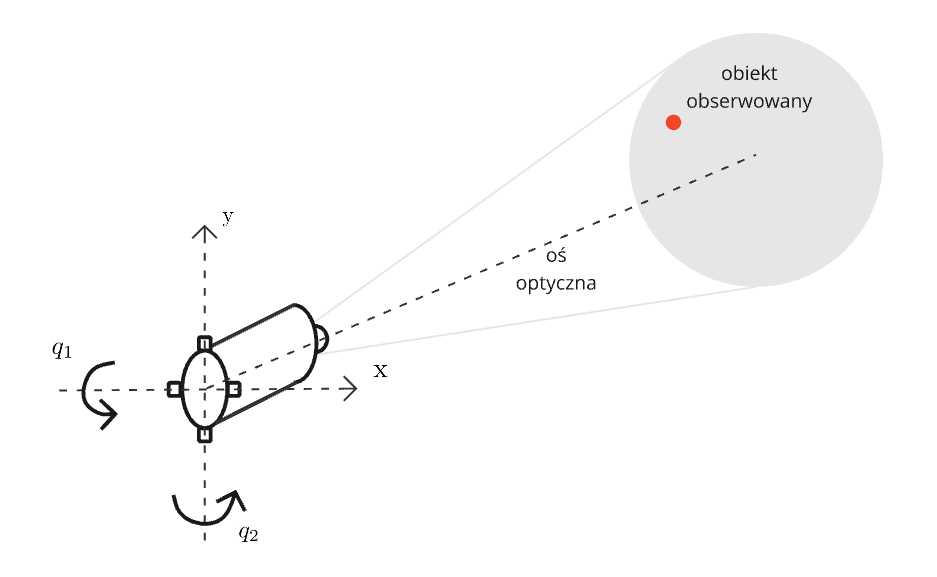
\includegraphics{testy/schematpogladowy.png}}
    \caption{Schemat poglądowy stanowiska badawczego}
    \label{fig:podglad5}
\end{figure}

\noindent Kąty te można interpretować jako dwa kąty Eulera opisujące orientację układu lokalnego względem układu podstawowego. Orientację tę można wyrazić za pomocą macierzy transformacji opisanych następująco: 

\begin{equation}
R_x(q_1) = 
\begin{bmatrix}
1 & 0 & 0\\
0 & \cos(q_1) & -\sin(q_1)\\
0 & \sin(q_1) & \cos(q_1)\\
\end{bmatrix},\ 
R_y(q_2) = 
\begin{bmatrix}
\cos(q_2) & 0 & \sin(q_2)\\
0 & 1 & 0 &\\
-\sin(q_2) & 0 & \cos(q_2)\\
\end{bmatrix},
\end{equation}
%
gdzie $R_x(q_1)$ i $R_y(q_2)$ określają elementarne obroty wokół osi X i Y układu lokalnego, przy czym kąty wyrażone są odpowiednio przez $q_1$ i $q_2$.
%\begin{center}
%\textit{Rotacja wokół %osi Y o $q_2$}
%\[
%\]}
%\textit{Rotacja wokół osi X o $q_1$}
Wypadkowa orientacja układu lokalnego wynika z następującego złożenia tych dwóch obrotów
%
\begin{equation}\label{eq:R_def}
R=R_x(q_1) \cdot R_y(q_2) =
\begin{bmatrix}
\cos(q_2) & 0 & \sin(q_2)\\
\sin(q_1) \sin(q_2) & \cos(q_1) & -\sin(q_1) \cos(q_2)\\
-\cos(q_1) \sin(q_2) & \sin(q_1) & \cos(q_1) \cos(q_2)\\
\end{bmatrix}.
\end{equation}
%
%określających obrót poszczególnych osi możliwe jest określenie położenia punktu w przestrzeni w odniesieniu do układu bazowego.
Przyjmując, że pozycja pewnego punktu w układzie lokalnym o orientacji początkowej zgodnej z układem podstawowym opisywana jest przez wektor $d=[d_x\ d_y\  d_z]^T\in\mathbb{R}^3$, to po wykonaniu obrotu opisanego przez \eqref{eq:R_def} jego pozycja w układzie podstawowym spełnia zależność
%
\begin{equation}
d^{'}=R \cdot d.    
\end{equation}
%
%
%wynosi $p^{T}=[p_x, p_y, p_z]$ i tym samym opisuje wektor kierunku $d^{T}=[d_x, d_y, d_z]$
%\textit{Macierz transformacji aktualnego położenie punktu względem układu}
%\noindent Po wyznaczeniu macierzy rotacji możemy obliczyć nowy wektor kierunku $p^'$ po rotacji oraz wyznaczyć nowe współrzędne punktu obserwowanego przez teleskop
%$d^{'}=R \cdot d$
%$$p^{'T}=[p_{x0}+d^{'}_{x}, p_{y0}+d^{'}_{y}, p_{z0}+d^{'}_{z}]$$

\noindent W tej pracy w roli elementu pozycjonującego  wykorzystano konstrukcję mechaniczną, której układ kinematyczny odpowiada przypadkowi zilustrowanemu na Rys.\ref{fig:podglad5}. Na Rys. \ref{fig:lkjlkjlkj} przedstawiono dwa widoki izometryczne konstrukcji, a na rys. \ref{fig:stan} jego widok rzeczywisty. 

\begin{figure}[!htb]
    \centering
    \resizebox{15cm}{!}{
    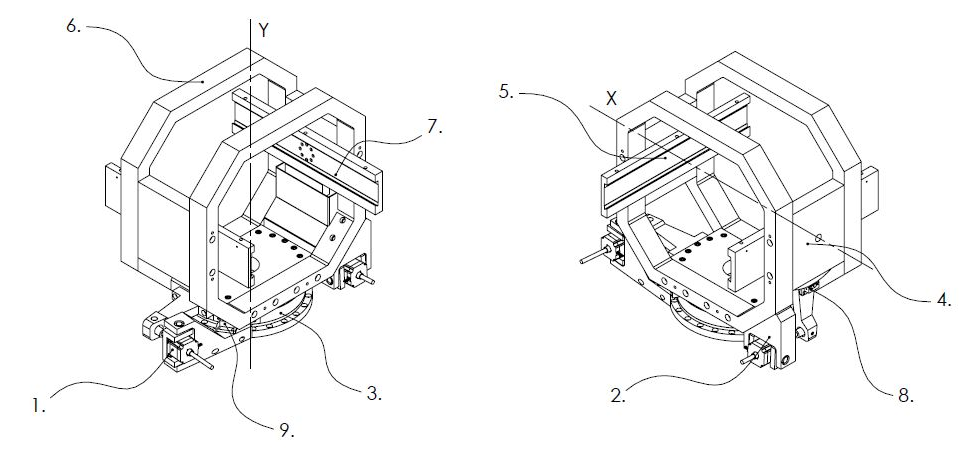
\includegraphics{pictures/lkjlkjlkj.png}}
    \caption{Widoki izometryczne stanowiska \cite{konstrukcja}}
    \label{fig:lkjlkjlkj}
\end{figure}

\begin{center}
    \begin{minipage}{0.45\textwidth}
        1. Układ napędowy osi X\\
        2. Układ napędowy osi Y\\
        3. Zespół łożyskowania osi Y\\
        4. Zespół łożyskowania osi X - węzeł napędowy\\
        5. Zespół łożyskowania osi X - węzeł swobodny
    \end{minipage}%
    \hspace{0.05\textwidth} 
    \begin{minipage}{0.45\textwidth}
        6. Klatka zespalająca\\
        7. Uchwyty mocujące teleskopy - złącze uniwersalne\\
        8. Układ pomiarowy obrotu osi X\\
        9. Układ pomiarowy obrotu osi Y
    \end{minipage}
\end{center}

\vspace{0.5cm}

\begin{figure}[!htb]
    \centering
    \resizebox{10cm}{!}{
    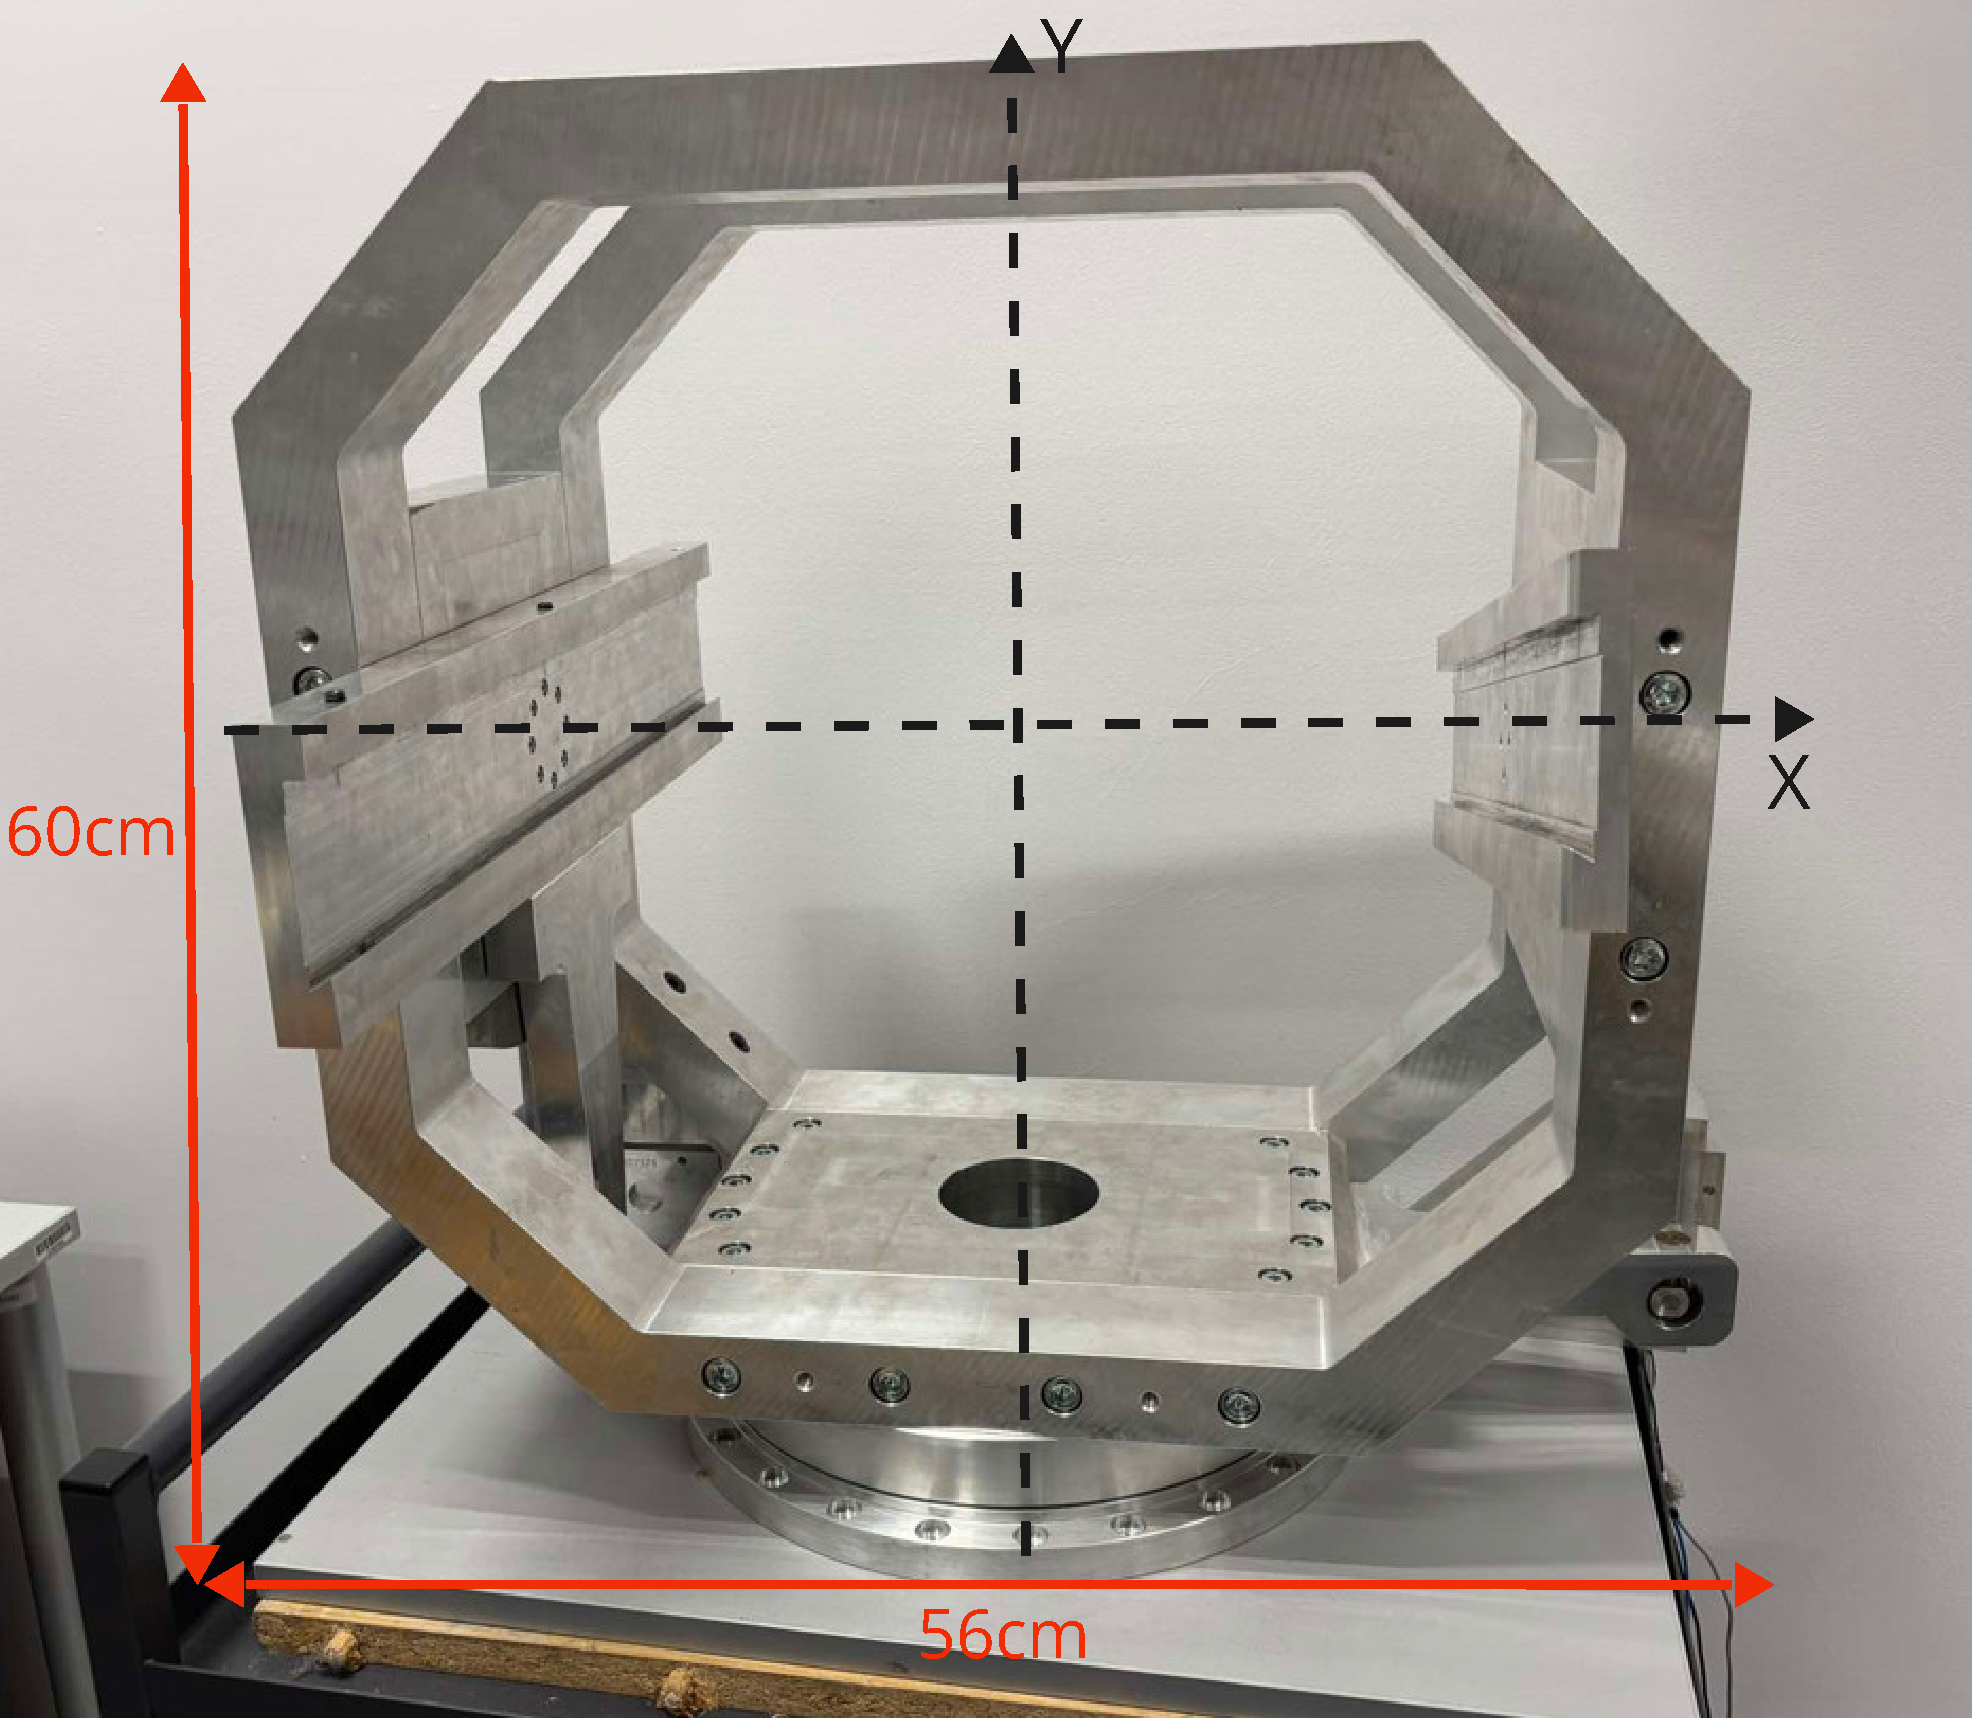
\includegraphics{pictures/Inżynierka (13).pdf}}
    \caption{Stanowisko w sali laboratoryjnej o wymiarach 56cm x 50cm x 60cm}
    \label{fig:stan}
\end{figure}

\vspace{1cm}

\begin{figure}[!htb]
    \centering
    \resizebox{10cm}{!}{
    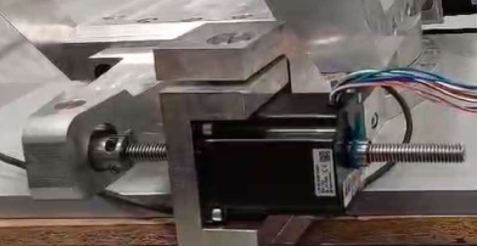
\includegraphics{pictures/przekladnia.png}}
    \caption{Silnik krokowy z przekładnią śrubową}
    \label{fig:śruba}
\end{figure}

\vspace{1cm}

\noindent Widoczne na rys. \ref{fig:śruba} połączenie z przekładnią śrubową silnika krokowego zapewnia precyzyjną konwersję ruchu obrotowego na liniowy umożliwiając uzyskanie bardzo dokładnego przesunięcia. Jest to spowodowane obrotem śruby, która porusza się z uwagi na oddziałujące na nią sprzęgło uzależnionego od połączonego z nim napędu. Dzięki właściwości samohamowności śruby trapezowej układ nie wymaga ciągłego podtrzymywania pozycji, a duża siła przesuwu jest osiągana nawet przy niewielkim momencie obrotowym silnika.

\newpage


% \chapter{Dobór elementów}
% \indent Na etapie projektowania układu sterowania uchwytem wyodrębnione zostały podstawowe bloki funkcjonalne przedstawione na rys. \ref{schematpogladowy}. Obejmują one między innymi czujniki pomiarowe takie jak enkodery będące częścią istniejącej konstrukcji mechanicznej, sterowniki silników krokowych oraz główne urządzenie zarządzające.

\begin{figure}[!htb]
    \centering
    \resizebox{16cm}{!}{
    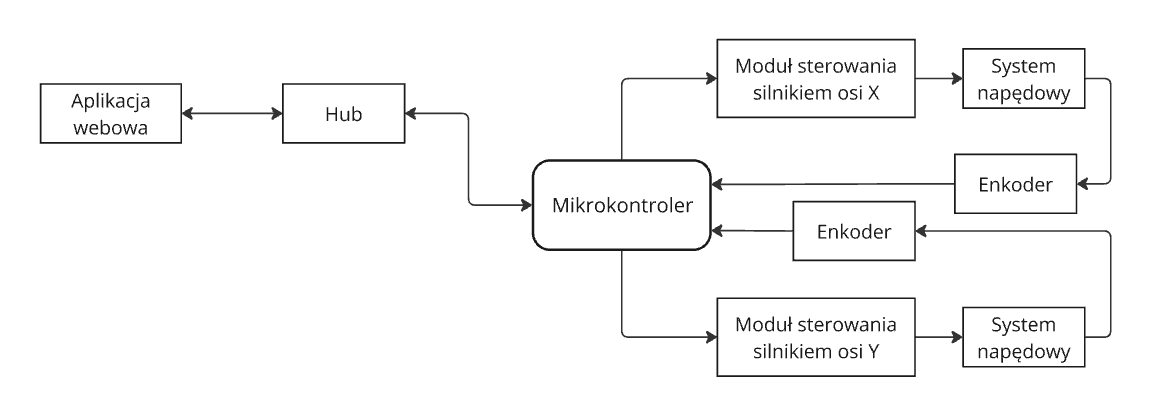
\includegraphics{testy/schematelementow.png}}
    \caption{Schemat elementów systemu}
     \label{schematpogladowy}
\end{figure}

\noindent Głównym elementem odpowiedzialnym za zarządzanie całym procesem jest mikrokontroler, pełniący rolę jednostki sterującej. Odbiera i przetwarza dane pochodzące z aplikacji webowej, w tym z warstwy frontendowej (interfejs użytkownika) oraz backendowej, którą w tym przypadku stanowi WebSocket. Ponadto odpowiada za komunikację zarówno z frontendem, jak i z serwerem działającym na STM32. Wymiana informacji między interfejsem użytkownika, a mikrokontrolerem STM32, odbywa się za pośrednictwem połączenia ethernetowego z protokołem TCP. Na STM32 działa serwer, który komunikuje się z urządzeniem sieciowym (hubem) i obsługuje przesył danych.

\noindent Po odebraniu i odpowiednim przetworzeniu danych z aplikacji webowej generowane są sygnały sterujące, które są przesyłane do modułów napędowych. Mikrokontroler wysyła kilka rodzajów sygnałów takich jak CLK (sygnał zegara), DIR (kierunek) oraz EN (zezwolenie na pracę), wpływając na działanie sterowników. Enkodery stanowiąc sprzężenie zwrotne za pośrednictwem interfejsu BISS-C, zwracają informacje do urządzenia sterującego, co pozwala na precyzyjne monitorowanie bieżącego stanu systemu. Silniki wraz z odpowiednią przekładnią tworząc system napędowy umożliwiają realizację zamierzonego ruchu, przekładając sygnały sterujące na odpowiednie obroty i moment obrotowy.

\noindent Mikrokontroler utrzymuje ruch platformy poprzez obliczanie zaimplementowanego algorytmu regulacji w celu ograniczenia uchybu kąta do przedziału wyznaczanego przez tzw. obszar tolerancji błędu (strefę nieczułości). Oznacza to, że system kontynuuje działanie, dopóki różnica między zadaną a rzeczywistą pozycją platformy przekracza określoną wartość progową. Taka konfiguracja pozwala na prostą realizację zadania sterowania przy ograniczeniu wrażliwości na błędy pomiarowe. Na etapie projektowania układu założono, że tak strategia powinna pozwolić uzyskać założony poziom dokładności. %płynne i stabilne %działanie całego układu, %zapewniając wysoką %dokładność oraz %skuteczność sterowania. 

%%%%%%%%%%%%%%%%%%%%%%%%%%%%%%%%%%% SILNIK %%%%%%%%%%%%%%%%%%%%%%%%%%%%%%%%%%%%%%

\section{Silniki}
Układ wykonawczy stanowi bardzo istotny element urządzenia pozycjonującego, dla którego opracowano układ sterowania. Konstrukcja  uchwytu oryginalnie została wyposażona w silniki krokowe, które choć nie zapewniają dużej dynamiki ruchu, to jednak umożliwiają precyzyjne sterowanie pozycyjne bez stosowania złożonego algorytmu pracującego w pętli zewnętrznej. Jest to uzyskiwane dzięki zasadzie działania tej grupy silników, które konstrukcyjnie zapewniają stabilne położenia wirnika

Z punktu widzenia działania układu istotne było dobranie odpowiedniej konfiguracji łączeniowej silników. Konfiguracje te obejmują: tryb unipolarny i tryb bipolarny w wersji szeregowej i równoległej - por. rys. \ref{fig:silnik}. 



%Z tego powodu przeanalizowano trzy sposoby podłączenia %\reviewdp{uzwojeń} silnika krokowego i wybrano \reviewdp{najlepszy}, dostosowany do warunków pracy. Wspomnijmy kilka słów na temat analizy wspomnianych wariantów.

\begin{figure}[!htb]
    \centering
    \resizebox{15cm}{!}{
    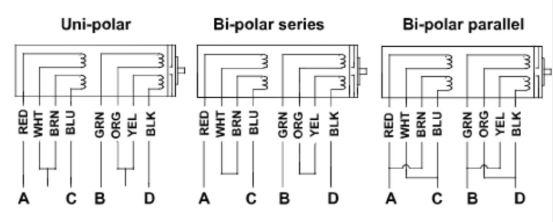
\includegraphics{pictures/silniki.png}}
    \caption{Sposoby podłączenia silników \cite{bipolarunipolar}}
    \label{fig:silnik}
\end{figure}

\begin{enumerate}
    \item \textbf{Połączenie unipolarne}\\
    Wyróżnia się z pewnością prostotą sterowania, a do jego prawidłowego działania wystarczy aktywować uzwojenia silnika w ustalonej kolejności. Zmiana kierunku obrotu wymaga jedynie odwrócenia sekwencji podawanego prądu. Pomimo swoich zalet jest ograniczone do generowania dużego momentu obrotowego. Z tego powodu nie stanowi odpowiedniego wyboru dla zastosowań wymagających większej siły np. obsługa dużej platformy.
    \item \textbf{Połączenie bipolarne szeregowe}\\
    W tym przypadku uzwojenia są połączone w taki sposób, że zwiększa się indukcyjność obwodu. Prowadzi to do ograniczenia stromości przepływu prądu przez uzwojenia, utrudniając pracę silnika przy wyższych częstotliwościach. Połączenie to generuje duży moment obrotowy, jednak ogranicza maksymalną prędkość obrotową. Jest ono odpowiednie dla aplikacji, gdzie wysoki moment jest priorytetem, a prędkość odgrywa mniejszą rolę.
    \vspace{1cm}
    \item \textbf{Połączenie bipolarne równoległe}\\
    Konfiguracja równoległa w połączeniu bipolarnym działa odwrotnie do połączenia szeregowego. Prąd dzieli się na dwa uzwojenia zmniejszając wpływ indukcyjności i pozwala na szybsze przełączanie faz w silniku. Dzięki temu silnik jest zdolny do pracy przy wyższych prędkościach, jednocześnie utrzymując relatywnie wysoki moment obrotowy. Spadek momentu wraz ze wzrostem prędkości nie jest tak gwałtowny jak w przypadku połączenia szeregowego czyniąc tę konfigurację bardziej uniwersalną dla szerokiego zakresu zastosowań.
\end{enumerate}

\vspace{1cm}

\noindent Warunki pracy rozważanego uchwytu wymagają użycia niewielkich prędkości obrotowych przy stosunkowo dużych wartościach momentu obrotowego \cite{silniki}. Z tego względu zdecydowano się na typ bipolarny szeregowy. \newline
\noindent Oprócz dobrania prawidłowej konfiguracji połączeń, praca silnika krokowego, a zwłaszcza precyzja pozycjonowania jego wirnika zależy od użytej strategii sterowania powiązanej z liczbą kroków w trakcie jednego obrotu. Można w tym obszarze wyróżnić pracę pełnokrokową (full step) lub pracę mikrokrokową (microstepping). Wariant \textbf{\textit{Full Step}} charakteryzuje się wykonywaniem pełnych kroków. Silnik wykorzystuje całkowity potencjał momentu obrotowego i z racji na mniej skomplikowane sterowanie pozwala uzyskać zwiększoną niezawodność. W przeciwieństwie do trybu pełnokrokowego działa \textbf{\textit{Mircostepping}} dedykowany dla odmiennego rodzaju implementacji. Zwiększona liczba położeń silnika względem osi obrotu pozwala osiągać dokładniejszą pozycję minimalizując błędy. Warto zauważyć, że z uwagi na większe rozproszenie płynącego prądu przez cewki zmniejsza się moment obrotowy utrudniając poruszanie rozbudowanych konstrukcji \cite{stepping}. Przykładowy możliwy podział kroków zaimplementowany w sterowniku Wobit SMC64BP pokazano na Rys.~ \ref{stepy}.

\begin{figure}[!htb]
    \centering
    \resizebox{12cm}{!}{
    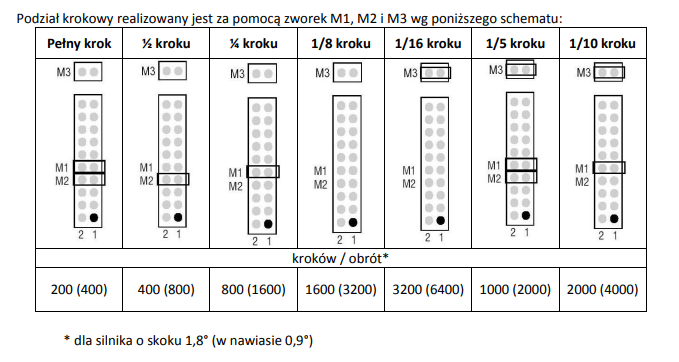
\includegraphics{pictures/stepy.png}}
    \caption{Tabelka z podziałami kroków drivera Wobit SMC64BP \cite{driver}}
    \label{stepy}
\end{figure}

%%%%%%%%%%%%%%%%%%%%%%%%%%%%%%%%%% SILNIK %%%%%%%%%%%%%%%%%%%%%%%%%%%%%%%%%%%%%%%

%%%%%%%%%%%%%%%%%%%%%%%%%%%%%%%%%% DRIVERY %%%%%%%%%%%%%%%%%%%%%%%%%%%%%%%%%%%%%%%
\section{Sterowniki silników krokowych} 

Do poruszania silnikami można użyć specjalizowanych układów wyposażonych we wzmacniacze mocy wraz z programowalnymi układami generującymi napięcia fazowe i ograniczającymi dopuszczalny prąd w uzwojeniach. Na rys. \ref{fig:driver} pokazano przykładowy cyfrowy interfejs sterujący \cite{driver2}. 

\begin{figure}[!htb]
    \centering
    \resizebox{13cm}{!}{
    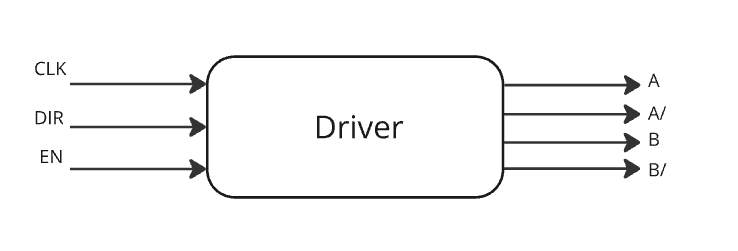
\includegraphics{pictures/driver.png}}
    \caption{Schemat blokowy sterownika}
    \label{fig:driver}
\end{figure}

\noindent Sygnał zezwolenia oznaczony jako \textbf{\textit{EN}} umożliwia działanie silnika pozwalając na przepływ prądu przez uzwojenia silnika. Wejście \textbf{\textit{DIR}} w zależności od swojego stanu określa kierunek obrotu silnika zgodnie lub przeciwnie do ruchu wskazówek zegara. Ostatnim z nich jest \textbf{\textit{CLK}}, który przyjmuje z urządzenia nadrzędnego sygnał PWM o danej częstotliwości definiując w ten sposób prędkość z jaką silnik ma się przemieszczać.\newline
\noindent Podczas realizacji pracy inżynierskiej użyte były dwa sterowniki silników oferowane przez firmę Wobit. Kontrolery SMC64 oraz SMC104 umożliwiają programowanie profili ruchu, określanie prędkości, przyspieszeń oraz docelowych pozycji dla każdego silnika. Dzięki temu SMC64 i SMC104 stanowią niezawodne i łatwe w utrzymaniu rozwiązania w środowiskach przemysłowych. Kontrolery mają możliwość obsługi różnych typów silników i oferują proste narzędzia do programowania, co sprawia, że są dosyć popularnym wyborem w aplikacjach wymagających dużej dokładności. Ich funkcje obejmują szeroki zakres zastosowań takich jak systemy CNC oraz systemy robotyki.

%%%%%%%%%%%%%%%%%%%%%%%%%%%%%%%%%% DRIVERY %%%%%%%%%%%%%%%%%%%%%%%%%%%%%%%%%%%%%%%

%%%%%%%%%%%%%%%%%%%%%%%%%%%%%%%%%% ENKODERY %%%%%%%%%%%%%%%%%%%%%%%%%%%%%%%%%%%%%%%
\section{Enkodery}
Enkodery to urządzenia służące do precyzyjnych pomiarów pozycji, kierunku ruchu wału lub innego obracającego się elementu. W zależności od metody wykonywania pomiarów, enkodery można podzielić na dwa główne rodzaje - enkodery optyczne inkrementalne i absolutne \cite{enkoder}.\newline 

\noindent Ze względu na swoją prostotę prawdopodobnie najczęściej spotykanym typem są enkodery inkrementalne. Ich działanie polega na generowaniu impulsów podczas obrotu obiektów. Enkoder inkrementalny składa się zazwyczaj z tarczy, na której znajdują się równomiernie rozmieszczone szczeliny lub ciemne i jasne segmenty, które przepuszczają lub blokują światło emitowane przez diodę LED. Światło pada na czujnik zliczający przejścia, generując w ten sposób impulsy. Każdy impuls odpowiada określonemu przemieszczeniu wału, co umożliwia obliczenie kąta obrotu oraz prędkości. Kolejnym istotnym elementem enkoderów inkrementalnych jest kanał referencyjny (kanał Z), który generuje impuls zerowy przy każdym pełnym obrocie wału. Ten pojedynczy impuls może być używany do ustalenia pozycji referencyjnej, co pozwala na wyzerowanie licznika i rozpoczęcie zliczania od tego punktu. Standardowe enkodery inkrementalne składają się z dwóch kanałów sygnałów (A i B), które są przesunięte względem siebie o 90 stopni (tzw. sygnały kwadraturowe). Dzięki temu możliwe jest określenie kierunku obrotu wału poprzez porównanie sygnałów A i B pozwalające ustalić, czy np. wał obraca się zgodnie z ruchem wskazówek zegara.\newline 
\noindent Enkodery absolutne różnią się od enkoderów inkrementalnych w sposobie definiowania pozycji wału, ponieważ każda pozycja takiego wału jest kodowana w sposób unikatowy. Dlatego, nawet jeśli zasilanie zostanie wyłączone, enkoder absolutny pamięta aktualną pozycję wału. Enkodery absolutne to enkodery z tarczą kodową, na której każda pozycja jest oznaczona charakterystycznym wzorem, który może być odczytywany przez różne czujniki. W zależności od zastosowanego kodu rozdzielczość enkodera absolutnego wynika z przyjętej reprezentacji kąta i liczby detektorów, umożliwiając precyzyjne określenie pozycji z dokładnością do ułamków stopnia. Sygnał wyjściowy jest reprezentowany przez liczby binarne lub inny kod cyfrowy, który definiuje konkretną pozycję. Taki kod może być kodem Gray’a, który minimalizuje błędy odczytu przy przełączaniu pomiędzy sąsiadującymi pozycjami. Z tego powodu enkodery absolutne są mniej podatne na zakłócenia i błędy w odczycie pozycji.\newline 
\noindent Ważnym aspektem w przypadku enkoderów jest pojęcie pozycji referencyjnej ustawionej ręcznie lub przez system sterujący. W inkrementalnym zwykle odbywa się to przez odnalezienie impulsu referencyjnego (kanał Z) generowanego raz na obrót. Po osiągnięciu tej pozycji system sterujący może zresetować licznik impulsów i rozpocząć zliczanie od zera. W enkoderach absolutnych nie ma potrzeby ustawiania pozycji referencyjnej, ponieważ każda pozycja jest odczytywana bezpośrednio jako unikatowa wartość eliminując potrzebę resetowania licznika.

\begin{figure}[!htb]
    \centering
    \resizebox{14cm}{!}{
    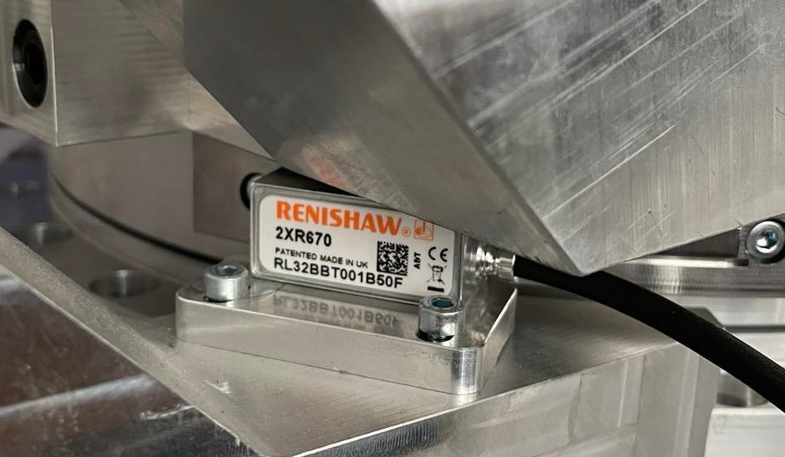
\includegraphics{pictures/enkoder.png}}
    \label{enkoder}
    \caption{Model zamontowanego enkodera na stanowisku}
\end{figure}

%%%%%%%%%%%%%%%%%%%%%%%%%%%%%%%%%% ENKODERY %%%%%%%%%%%%%%%%%%%%%%%%%%%%%%%%%%%%%%%

%%%%%%%%%%%%%%%%%%%%%%%%%%%%%%%%%% MIKROKONTROLER %%%%%%%%%%%%%%%%%%%%%%%%%%%%%%%%%%%%%%%
\section{Mikrokontroler}
Podstawowym elementem układu sterowania uchwytem odpowiedzialnym za odczyt z pozycji, obsługę sterowników silników, realizacji algorytmu sterowania pozycyjnego potrzebne było urządzenie wielofunkcyjne. Z ogólno dostępnych i tanich rozwiązań zdecydowaliśmy się na minikomputer, a dokładniej model płytki programistycznej STM32H743ZI z zaawansowaną platformą deweloperską opartą na mikrokontrolerze z serii STM32H7 zaprojektowaną przez firmę STMicroelectronics. Miktrokontrolery te charakteryzują się dużą wydajnością, wysoką częstotliwością taktowania oraz rozbudowanymi możliwościami komunikacyjnymi, co sprawia, że są idealnym rozwiązaniem do zastosowań wymagających dużej mocy obliczeniowej oraz wszechstronnej komunikacji. Wspomniany rodzaj płytki programowalnej STM32 Nucleo-144 oferuje bardzo wysoką wydajność obliczeniową dzięki rdzeniowi ARM Cortex-M7 działającemu z częstotliwością nawet do 480 MHz. Zawiera również bogaty zestaw peryferiów i dużą ilość pamięci (do 2 MB Flash oraz 1 MB RAM). Ponadto, STM32H743ZI oferuje szereg funkcji, które znacząco ułatwiają proces projektowania oraz integracji aplikacji takich jak zintegrowany debugger/programmer ST-LINK eliminując potrzebę stosowania zewnętrznych narzędzi do debugowania i programowania. Jest to duże udogodnienie przyspieszające proces rozwoju i testowania aplikacji. \newline 
\noindent Płytka STM32 Nucleo-144 oferuje też pełną kompatybilność z popularnym standardem ARDUINO® Uno V3 pozwalając na łatwą integrację z szeroką gamą dostępnych rozszerzeń odnoszących sie do płytek nasadkowych tzw. shields. Dodatkowo, złącza ST morpho oraz Zio zapewniają jeszcze większe możliwości rozbudowy płytki o dodatkowe moduły i peryferia. Z kolei, dzięki złączu MIPI20 można podłączyć moduły kamer, co może być istotnym elementem w projektach związanych z przetwarzaniem obrazu lub monitorowaniem wideo. \newline 
\noindent Wspomniany model udostępnia interfejsy komunikacyjne, w tym Ethernet (RJ45), USB w wersjach pełnej prędkości oraz USB OTG pozwalając na łatwą komunikację z innymi urządzeniami. Jednocześnie zawiera również interfejsy komunikacyjne takie jak I2C lub SPI zdatnych do pobierania informacji z urządzeń takich jak chociażby enkodery. \newline
\noindent Warto także nadmienić, że mikronkontroler wspiera bogaty ekosystem oprogramowania STM32Cube, który obejmuje biblioteki, przykłady kodu oraz narzędzia do konfiguracji peryferiów. Dodatkowo, płytka wspiera popularne systemy operacyjne czasu rzeczywistego FreeRTOS, co jest przydatne w bardziej zaawansowanych aplikacjach wspomagających między innymi pracę serwera sieciowego.

%%%%%%%%%%%%%%%%%%%%%%%%%%%%%%%%%% MIKROKONTROLER %%%%%%%%%%%%%%%%%%%%%%%%%%%%%%%%%%%%%%%

%%%%%%%%%%%%%%%%%%%%%%%%%%%%%%%%%% SWITCH/HUB %%%%%%%%%%%%%%%%%%%%%%%%%%%%%%%%%%%%%%%
\section{Switch/Hub}
Switch i Hub stanowią urządzenia sieciowe służące do łączenia komputerów i innych urządzeń w sieciach lokalnych nazywanych. Pomimo podobnej funkcji oraz wzajemnego wpływu na efektywność i wydajność sieci różnią się sposobem działania. \cite{net}.\newline
\noindent Huby to prostsze i z reguły tanie sprzęty sieciowe, które działają jako punkt rozdzielający sygnał sieciowy. Wszystkie urządzenia podłączone do hub-a są ze sobą połączone w sposób równoległy. Kiedy transmitter wysyła dane hub przekazuje ten sygnał do wszystkich portów. Nie analizuje adresów docelowych, dlatego każde urządzenie w sieci otrzymuje dane, nawet jeśli nie są one do niego skierowane. Receivery są więc zmuszone zignorować dostaroczne do nich pakiety informacji. \newline
\noindent W przeciwieństwie do hubów switche to bardziej zaawansowane urządzenie sieciowe, które działają na wyższej w warstwie łącza danych modelu OSI, czyli na warstwie drugiej. Analizują adresy MAC urządzeń podłączonych w jego porty i definiują wewnętrzną tablicę MAC, według której następuje przesył pakietów. Gdy dane docierają do switch-a sprawdza on adres MAC docelowy wysyłając dane bezpośrednio do odpowiedniego portu, zamiast rozsyłać je do wszystkich urządzeń. Dzięki temu switch minimalizuje ruch w sieci i zwiększa wydajność, ponieważ tylko właściwe urządzenie odbiera dane. \newline
\noindent W naszej aplikacji jedynym urządzeniem odbierającym dane z serwera jest mikrokontroler. Aspekt wydajności nie był najważniejszy, dzięki czemu można było wybrać podstawową opcję, czyli hub. 

%%%%%%%%%%%%%%%%%%%%%%%%%%%%%%%%%% SWITCH/HUB %%%%%%%%%%%%%%%%%%%%%%%%%%%%%%%%%%%%%%%
\newpage 

% \chapter{Sterowanie}
% \input{konfiguracja}

% \chapter{Komunikacja z enkoderem}
% %%%%%%%%%%%%%%%%%%%%%%%%%%%%%%%%%% TEORIA %%%%%%%%%%%%%%%%%%%%%%%%%%%%%%%%%%%%%%%
\section{Protokół komunikacyjny BISS-C}
Bidirectional Synchronous Serial - Continuous mode to otwarty standard komunikacji szeregowej zaprojektowany z myślą o enkoderach absolutnych. Chcąc odczytać pozycję z ich pomocą wykorzystuje się połączenie fizyczne będące skrętką dwużyłową do transmisji danych i impulsów zegarowych (MA i SL). Dzięki temu możliwe jest przesyłanie sygnałów na większe odległości bez znaczących strat jakości. Ten rodzaj komunikacji wykorzystywany jest szczególnie w systemach automatyki przemysłowej i precyzyjnego sterowania ruchem. Działa w układzie transmitter-receiver, w którym urządzenie nadrzędne pełniąc rolę odbiorcy zarządza czasem transmisji, a enkoder pełni rolę urządzenia wysyłającego dane w odpowiedzi na impulsy zegarowe. \newline 
\noindent BiSS-C oferuje stosunkowo wysoką szybkość transmisji danych osiągającą nawet 10 MHz. Dane są przesyłane w formacie binarnym, z możliwością wyboru długości słowa od 18 do 36 bitów. Oprócz danych opisujących pozycję, enkodery mogą przesyłać dodatkowe informacje diagnostyczne, takie jak bity ostrzeżeń lub błędów, co umożliwia bieżące monitorowanie stanu urządzenia. Zapewnia również integralność transmisji poprzez mechanizm kontroli błędów oparty na 6-bitowej sumie kontrolnej CRC.\cite{bissC}. 

\begin{figure}[!htb]
    \centering
    \resizebox{16cm}{!}{
    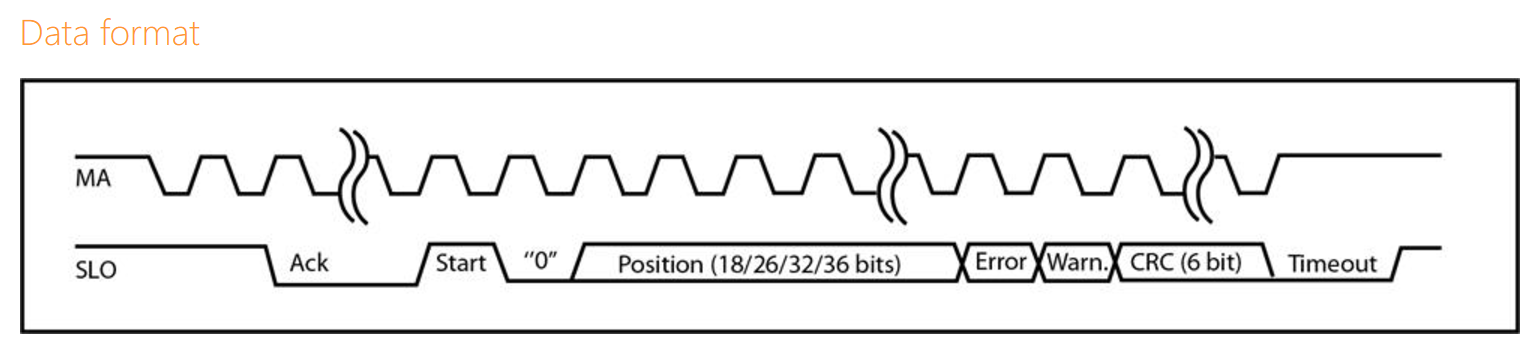
\includegraphics{pictures/ramka)danych.png}}
    \label{fig:PPLogo}
    \caption{Ramka danych protokołu Biss-C \cite{bissC2}}
\end{figure}

\noindent Dodatkową zaletą protokołu jest jego odporność na zakłócenia elektromagnetyczne czyniąc go odpowiednim rozwiązaniem nawet w trudnych warunkach przemysłowych. Istnieją również wersje rozszerzone tego protokołu zalecane do wykorzystania ze względu na bezpieczeństwo. Takim przykład jest rodzaj BiSS Safety umożliwiający spełnienie rygorystycznych norm, w tym ISO 13849 oraz IEC 61508 \cite{normy}. 

%%%%%%%%%%%%%%%%%%%%%%%%%%%%%%%%%% TEORIA %%%%%%%%%%%%%%%%%%%%%%%%%%%%%%%%%%%%%%%

%%%%%%%%%%%%%%%%%%%%%%%%%%%%%%%%%% TEORIA2 %%%%%%%%%%%%%%%%%%%%%%%%%%%%%%%%%%%%%%

%%%%%%%%%%%%%%%%%%%%%%%%%%%%%%%%%% TEORIA2 %%%%%%%%%%%%%%%%%%%%%%%%%%%%%%%%%%%%%%

%%%%%%%%%%%%%%%%%%%%%%%%%%%%%%%%%% KOD %%%%%%%%%%%%%%%%%%%%%%%%%%%%%%%%%%%%%%%
\section{Implementacja w programie}

\indent Z uwagi na budowę ramki do odczytu danych z enkodera zaimplementowano kod oddzielający kolejne sekcje krok po kroku. Poszczególne zbiory bitów zapisywanie w zależności od taktowania sygnału zegarowego są wyłapywane przez funkcje utworzone w programie powstałego na podstawie algorytmu odbierania danych z rys. \ref{fig:Blank board (1)}:

\begin{figure}[!htb]
    \centering
    \resizebox{14cm}{!}{
    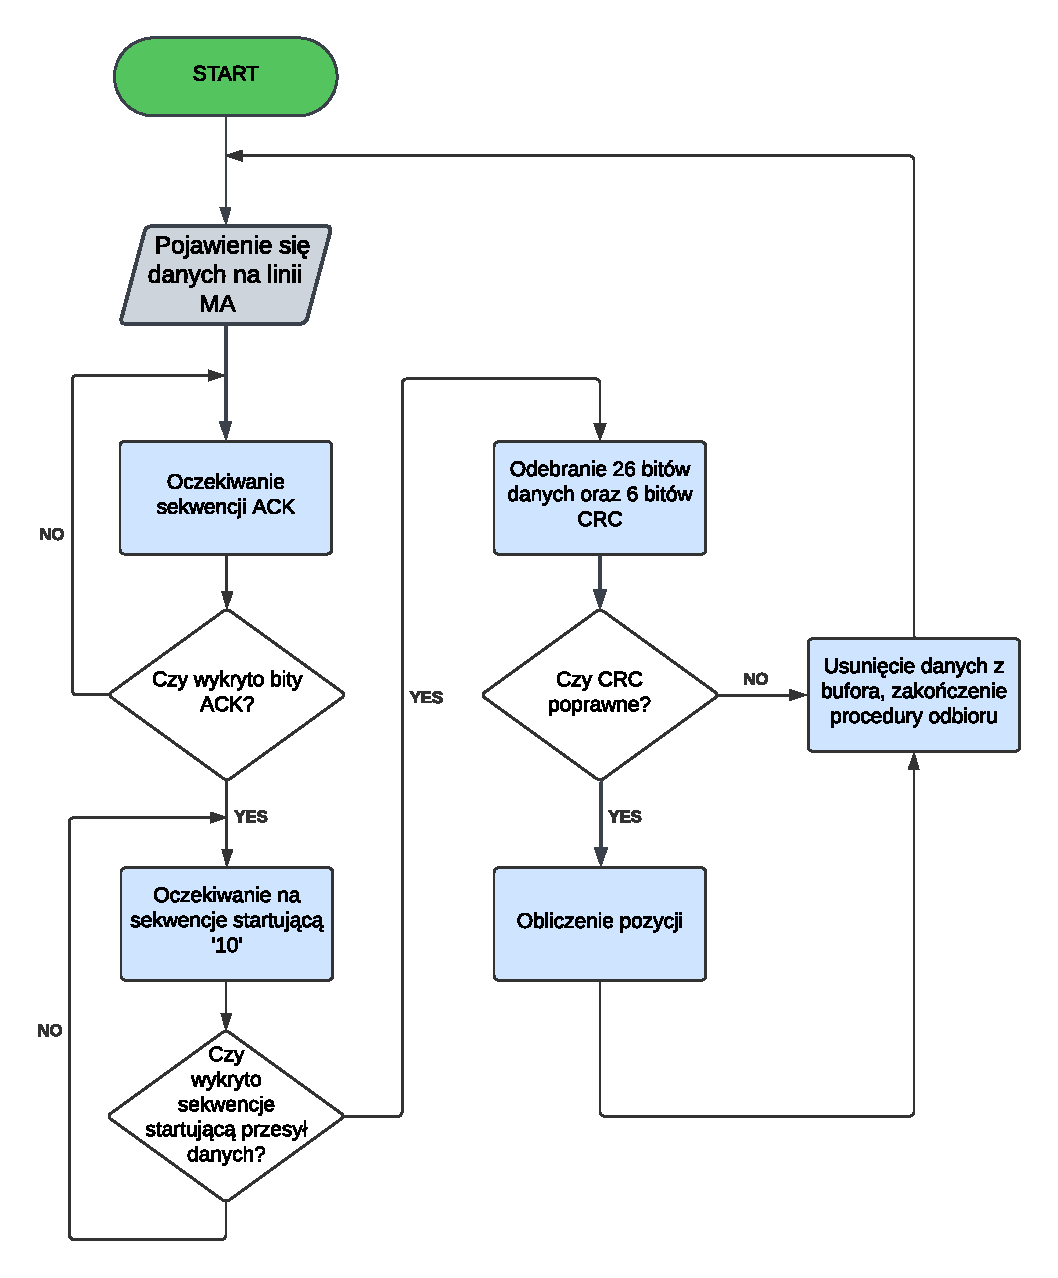
\includegraphics{pictures/Blank board (2).pdf}}
    \caption{Algorytm odbioru danych z enkodera}
    \label{fig:Blank board (1)}
\end{figure}

\vspace{0.5cm}

\newpage 

\begin{center}
    \textbf{Opis algorytmu}
\end{center}

\vspace{0.5cm}

\begin{enumerate}
    \item Oczekiwanie sekwencji ACK \newline
    Program nasłuchuje linię danych i czeka na pierwszą część ramki, czyli kod ACK. W naszym przypadku funkcja za to odpowiedzialna iteruje 8 możliwych przesunięć bitowych pierwszego bajtu bufora danych szukając miejsca, w którym sygnał wysoki z linii zmieni się na niski. Dokładniej, wynik przesunięcia jest sprawdzany z maską 0x80 w ramach operacji logicznej XOR oczkując rezultatu 0x00. Następnie ustawia zmienną programową o nazwie \textit{isAckDetected} na 1, co pozwala przejść dalej w działaniu programu

\vspace{0.5cm}

    \item Wyznaczanie bitu startu \newline
    W tym przypadku przechodzimy do znalezienia indeksu bajtu, od którego zaczyna się właściwa ramka danych poszukując początkowego wzorca bitowego $10$. Iterując cały bufor danych od momentu wykrycia ACK funkcja szuka pierwszego bajtu, który jest różny niż 0x00 stanowiąc prawdopodobnie początek głównych danych potrzebnych do odczytania położenia.

\vspace{0.5cm}
    
    \item Przesunięcie ramki bitów \newline
    Obliczane jest przesunięcie bitowe potrzebne do prawidłowego odczytu danych oraz weryfikuje początek ramki. Początkowo funkcja zaczyna sprawdzać czy poprawnie wykryto bit startu po przesunięciu ramki do indeksu z poprzedniego kroku. Sprawdza następne dwa bity $10$ za pomocą maski 0xC0, aby upewnić się, czy początek ramki jest poprawny. Jeśli początek został wykryty, flaga programowa \textit{isStartDetected} ustawia się na 1 i obliczane jest dokładne przesunięcie. Do indeksu danych dodaje się wartość 2 w celu odczytania bitów danych.

\vspace{0.5cm}
    \item Przypisanie bitów do bufora \newline 
    Przypisuje dane do struktury reprezentującej ramkę danych. Iteruje przez długość bufora ramki z enkodera przesuwając odpowiednie fragmenty danych oraz przypisując bity do docelowej struktury danych gotowej do przeliczania aktualnego położenia. Każdy element bufora ramki jest składany z dwóch sąsiednich bajtów enkodera, uwzględniając przesunięcie bitowe. Następnie cała ramka danych jest kopiowana do struktury za pomocą rzutowania.

\vspace{0.5cm}
    \newpage
    \item Obliczanie pozycji \newline
     Funkcja oblicza rzeczywistą pozycję enkodera, uwzględniając kalibrację mechaniczną i parametry enkodera. Spośród pozyskanej ramki danych wartość surowa wartości położenia zostaje zdekodowana oraz przemnożona przez współczynnik konwersji impulsów odczytanego z dokumentacji technicznej urządzenia. Końcowa wartość pozycji zostaje skorygowana o ustawiony wcześniej offset oraz przypisana do zmiennej wspomagającej sterowanie.

\vspace{0.5cm}

    \item Obliczanie sumy CRC \newline
    W celu kontroli poprawności ramki danych obliczona zostaje suma CRC, której wartość decyduje o odrzuceniu otrzymanego wyniku w zależności od ustawionej kombinacji.    
\end{enumerate}

\newpage

%%%%%%%%%%%%%%%%%%%%%%%%%%%%%%%%%% KOD %%%%%%%%%%%%%%%%%%%%%%%%%%%%%%%%%%%%%%%

% \chapter{Komunikacja pomiędzy mikrokontrolerem, a aplikacją webową}
% \section{Wybranie technologii aplikacji}
Do komunikacji z mikrokontrolerem została wybrana aplikacja webowa. Jest to nowoczesne i wygodne rozwiązanie. Do obsługi aplikacji została wybrana biblioteka języka JavaScript React, która została opisana w sekcji \ref{section:React}. Zapewnia ona obsługę dynamicznego interfejsu użytkownika.
Z uwagi na to, że przeglądarki nie obsługują połączeń z urządzeniami w sieci przez protokół TCP z powodów bezpieczeństwa, konieczne było użycie pośrednika. Do komunikacji pomiędzy frontendem i backendem aplikacji została wybrana technologia WebSocket.
WebSocket przyjmuje dane z przeglądarki, wysyła je do mikrokontrolera sterującego osiami, dostaje od niego odpowiedź, a następnie otrzymaną odpowiedź przesyła z powrotem do aplikacji. WebSocket został utworzony przy użyciu środowiska uruchomieniowego JavaScript Node.js, które zostało opisane w sekcji \ref{section:Node.js}. Do poprawnego działania aplikacji i WebsSocketu potrzeba zarówno Node.js jak i  menedżer pakietów NPM, które zostało opisane w sekcji \ref{section:NPM}. Przykład przepływu danych został pokazany na schemacie blokowym \ref{fig:schemat blokowy komunikacji ogolny}.
\begin{figure}[H]
    \centering
    \resizebox{15.5cm}{!}{
    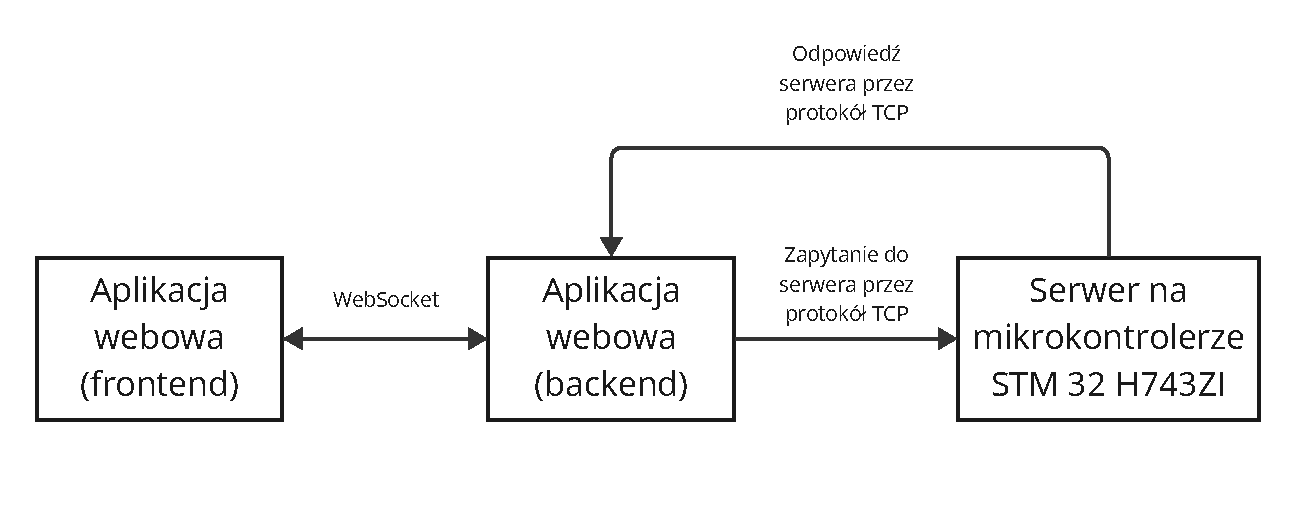
\includegraphics{interface/schemat blokowy.pdf}}
    \caption{Schemat blokowy wymiany danych.}
    \label{fig:schemat blokowy komunikacji ogolny}
\end{figure}
\section{Właściwości TCP}
Protokół TCP posiada wiele zalet:
\begin{enumerate}
    \item \textbf{Niezawodność przesyłu danych:} protokół TCP gwarantuje przesył danych do odbiorcy w oryginalnej formie. Wykorzystuje takie mechanizmy jak numeracja sekwencyjna, potwierdzenie ACK (odbiorca potwierdza otrzymanie pakietu) i retransmisje. W przypadku utraty pakietu, zostanie on przesłany ponownie, aż do otrzymania pełnych danych.
    \item \textbf{Komunikacja dwukierunkowa:} TCP polega na komunikacji dwukierunkowej. Dzięki czemu obydwie strony mogą przesyłać dane. Jest to przydatne w celu potwierdzenia czy odbiorca otrzymał pakiety.
\end{enumerate}
Oprócz swoich korzyści powszechnie stosowany protokół TCP niesie ze sobą niebezpieczeństwa, które mogą go wykluczyć z użytku w aplikacjach.
\begin{enumerate}
    \item \textbf{Podatność na ataki:} jednym z możliwych ataków jest man-in-the-middle, który może prowadzić do przechwycenia i modyfikacji danych bez wiedzy serwera i klienta. Innym przykładem jest atak typu TCP spoofing, polega on na podszyciu się pod innego użytkownika, wysyłając pakiety TCP z fałszywym IP. Może to prowadzić do przechwycenia wrażliwych danych lub złośliwego wstrzyknięcia poleceń.
    \item \textbf{Brak szyfrowania:} protokół TCP nie ma wbudowanego mechanizmu szyfrowania, ani autoryzacji. W związku z tym dane mogą być narażone na podsłuch przez osoby trzecie.
\end{enumerate}
Aplikacja webowa działa tylko lokalnie, dlatego nie trzeba rozpatrywać kwestii bezpieczeństwa. Dobrze zabezpieczona sieć rozwiązuje powyższe problemy.
\section{React}
\label{section:React}
Do zaprogramowania frontendu aplikacji webowej został wybrany React \cite{React}. Jest to biblioteka JavaScript, stworzona i rozwijana przez firmę Meta (dawniej Facebook), która służy do budowania interfejsów użytkownika. Główną zaletą React'a jest obsługa złożonych i dynamicznych aplikacji webowych poprzez użycie komponentów, które mogą być wielokrotnie używane.

\subsection{Działanie Reacta}
React działa według zasady \textbf{Virtual DOM} opisanej w sekcji \ref{section:Virtual DOM}, co oznacza, że zmiany w interfejsie użytkownika są najpierw dokonywane w specjalnej wirtualnej reprezentacji DOM, a dopiero potem synchronizowane z rzeczywistym DOM, co znacznie zwiększa wydajność aplikacji.
\subsection{Zalety Reacta}

\begin{enumerate}
    \item \textbf{Komponenty wielokrotnego użytku}: React pozwala na budowanie aplikacji za pomocą małych izolowanych komponentów, które są zaprojektowane do wielokrotnego użytku i łatwego zarządzania.
    \item \textbf{Wysoka wydajność}: React zawdzięcza swoją wydajność dzięki Virtual DOM. React minimalizuje liczby operacji na rzeczywistym DOM, co przekłada się na wysoką wydajność i szybkość działania aplikacji.
    \item \textbf{Popularność i wsparcie}: React jest popularny na skale światową co wpływa na ogromną społeczność developerów, którzy udostępniają dużą ilość bibliotek, narzędzi oraz wsparcia w przypadku luk w bibliotekach.
    \item \textbf{Możliwość używania JSX}: Jednym z największych plusów React'a jest JSX, rozszerzenie składni JavaScriptu, który umożliwia pisanie kodu podobnego do HTML co znacząco ułatwia tworzenie komponentów i zarządzanie nimi.
    \item \textbf{Ekosystem}: React posiada bogaty ekosystem, w tym React Hooks, który znacznie ułatwia zarządzanie stanem aplikacji.
\end{enumerate}

\subsection{React Hooks}
Hooki to funkcje, które zostały wprowadzone do React od wersji 16.8 i pozwalają na używanie kontroli stanu oraz innych funkcji w komponentach funkcyjnych. Wcześniej całe komponenty trzeba było pisać w klasach, co znacząco utrudniało minimalizm przy małych komponentach. Dzięki hook'om można w prosty sposób zarządzać komponentami.

\begin{enumerate}
    \item \textbf{useState}: pozwala na zarządzanie stanem w komponencie funkcyjnym. Przechowuje aktualne dynamiczne dane, takie jak wprowadzony tekst czy stan przycisku. W aplikacji webowej jest między innymi używany do przechowywania próbek, informacji o pozycji w polach tekstowych czy o stanie przycisku. W przypadku zmiany stanu, komponent w którym został zmieniony stan, jak i komponenty dzieci (ang. \textit{children}), zostaną przeładowane. W przypadku zbyt dużej ilości dzieci, może dojść do problemu z wydajnością. W aplikacji ilość dzieci została ograniczona, dodatkowo zostały zastosowane inne techniki optymalizacyjne, które zostaną opisane w następnych punktach.
    
    \item \textbf{useEffect}: służy do zarządzania efektami ubocznymi w komponencie. Efekty uboczne to operacje, które mają wpływ na zewnętrzne środowisko komponentu. W kontekście wykresów, chodzi o zmianę jednostki i zmianę aktualnych próbek. Jeśli chodzi o główną część aplikacji, to useEffect obsługuje połączenie się z WebSocketem jak i zamknięciem komunikacji.
    
    \item \textbf{useMemo}: służy do optymalizacji wydajności poprzez zapamiętywanie wyników kosztownych obliczeń. Dzięki temu nie musimy co każde odświeżenie stanu ponownie obliczać niektórych danych np. takich jak przekształcenie próbek na inne jednostki np. na radiany. Ten hook działa jak pamięć podręczna dla obliczeń. Ponowne obliczenie tych wartości zachodzi przy zmianie zależności.
    
    \item \textbf{useRef}: pozwala na tworzenie odwołań do elementów DOM oraz przechowywania zmiennych. Różni się od useState tym, że nie wywołuje ponownego przeładowania komponentu. W tym przypadku jest przechowywane połączenie z WebSocketem.
\end{enumerate}
\subsection{React-plotlyjs}
React-plotly.js to biblioteka umożliwiająca integrację biblioteki Plotly.js z Reactem. Służy ona do wizualizacji danych z aplikacjami stworzonymi w React. Umożliwia ona tworzenie zaawansowanych i interaktywnych wykresów, które można w bardzo prosty sposób zarządzać i dynamicznie zmieniać wyświetlane dane na wykresie za pomocą React.
\subsection{Działanie React-plotly}
React-plotly.js oferuje komponent Reactowy, który opiera się na Plotly.js. Wykorzystuje właściwości props, czyli danych o specjalnym kluczu, do definiowania danych, wyglądu i funkcji interaktywnych wykresów. Dzięki tym narzędziom można w prosty sposób sposób zmieniać dane jak i wygląd wykresów. W aplikacji jest możliwość zmiany jednostek, wspomniana wcześniej biblioteka w prosty sposób umożliwia modyfikacji opisów osi jak i zamianę danych na wykresie.
\subsection{Zalety react-plotlyjs}
\begin{enumerate}
    \item \textbf{Interaktywność:} Zapewnia interaktywne funkcje, takie jak powiększanie, przesuwanie, tooltipy i zapis wykresu.
    \item \textbf{Integracja z React:} Dzięki komponentowi plotly.js można w prosty sposób zarządzać dynamicznie stanem wykresów. W tym przypadku cały czas wykresy są aktualizowane z aktualną pozycją rotorów jak i uchybem.
    \item \textbf{Wydajność:} W aplikacji jest wgrywanych, na pojedynczy wykres, co sekundę aż 1 000 nowych próbek, co w znaczny sposób obciąża aplikację. Jednym ze sposobów polepszenia wydajności jest zastosowanie WebGL, poprzez typ wykresu scatterg, co znacząco polepsza wydajność przy renderowaniu wykresów.
    \item \textbf{Eksport danych:} Umożliwia eksport wykresów w formacie PNG.
\end{enumerate}
Standardowe wykresy rozproszone w Plotly.js (\textit{scatter}) wykorzystują SVG do renderowania punktów i linii, co jest efektywne dla małych i średnich zbiorów danych. Na wykresach jest ładowana duża ilość próbek, która może być liczona w milionach przez co w tym przypadku renderowanie za pomocą SVG jest niewydajne. W takich przypadkach wykorzystuje się scattergl, który wykorzystuje WebGL.
Jednym z minusów scattergl jest mniejsza ostrość, ponieważ wykres nie jest renderowany wektorowo.
\section{Komunikacja z aplikacji webowej do STM32}
Do komunikacji jako schemat wiadomości został wybrany \textbf{JSON} (JavaScript Object Notation). JSON jest lekkim formatem danych, który jest zarówno łatwy do odczytania jak i rozszerzenia w razie potrzeby przesłania większej ilości danych. Został szerzej opisany w sekcji \ref{section:JSON}. Przykład komunikacji został przedstawiony na schemacie blokowym \ref{fig:schemat blokowy komunikacji z aplikacji webowej do serwera na STM32}.
\begin{lstlisting}[caption=Przykład struktury JSON z aplikacji webowej do STM32]
{
  "isFetching": 0 || 1,
  "isEngineEnabled": 0 || 1,
  "positionX": int,
  "positionY": int,
  "mode": int {0, 1, 2}
}
\end{lstlisting}
Oznaczenie \textbf{0 || 1} reprezentuje wartości logiczne \textbf{0} (fałsz) lub \textbf{1} (prawda). 
Takie podejście wynika z faktu, że język C domyślnie nie posiada wbudowanego typu \textbf{bool}. 
W przypadku STM32 oraz biblioteki cJSON, opisanej w sekcji \ref{section:cJSON}, dostępne są ich własne implementacje typu logicznego (bool). 
Aby zintegrować obie technologie, znacznie łatwiej jest obsługiwać wartości logiczne jako numeryczne typu \textbf{int}.
\begin{enumerate}
    \item \textbf{isFetching}: informacja dla mikrokontrolera czy ma zapamiętywać odczytaną pozycję w pamięci. W przypadku wartości 1 próbki będą zapisywane w buforze. Analogicznie, dla wartości 0 próbki nie będą zapisywane.
    \item \textbf{isEngineEnabled}: w przypadku wartości 1, obydwa silniki krokowe sterujące osiami się załączą, również aktywuje się możliwość zmiany stanu \textit{CLK}. Analogicznie w przypadku wartości 0 sygnały \textit{CLK} nie będą zmieniać stanu jak i sygnały \textit{ENABLED} będą ustawione na stan niski. Jest to niezwykle przydatne w celu ograniczenia zużycia energii przez silniki jak i przez sterownik w stanie bezczynności.
    \item \textbf{positionX, positionY}: wartość zadana dla osi X i Y, które odpowiadają kątom $q_1$ i $q_2$. Wartość jest przesyłana w formacie \textbf{RAW}, czyli taką jaką enkoder odczytuje. Przesyłanie pozycji w tej formie jest najprostszym rozwiązaniem, ponieważ nie musimy na mikrokontrolerze przetwarzać wartości na inny format. Podczas sterowania silnikiem sprawdzamy aktualną pozycję enkodera, dlatego ustawienie wartości zadanej w tych samych jednostkach, co pomiary dostarczane przez enkoder, ogranicza zamianę wartości na inny format i unika błędów obliczeniowych podczas zamiany formatu. 
    \item \textbf{mode:} tryb sterowania osiami. Dla następujących wartości osie przyjmują następująca trajektorię:
    \begin{itemize}
        \item 0: punkt. Różne wartości punktowe dla dwóch osi.
        \item 1: sinusoidalną.
        \item 2: prostokątną.
    \end{itemize}
\end{enumerate}

\begin{figure}[H]
    \centering
    \resizebox{15.5cm}{!}{
    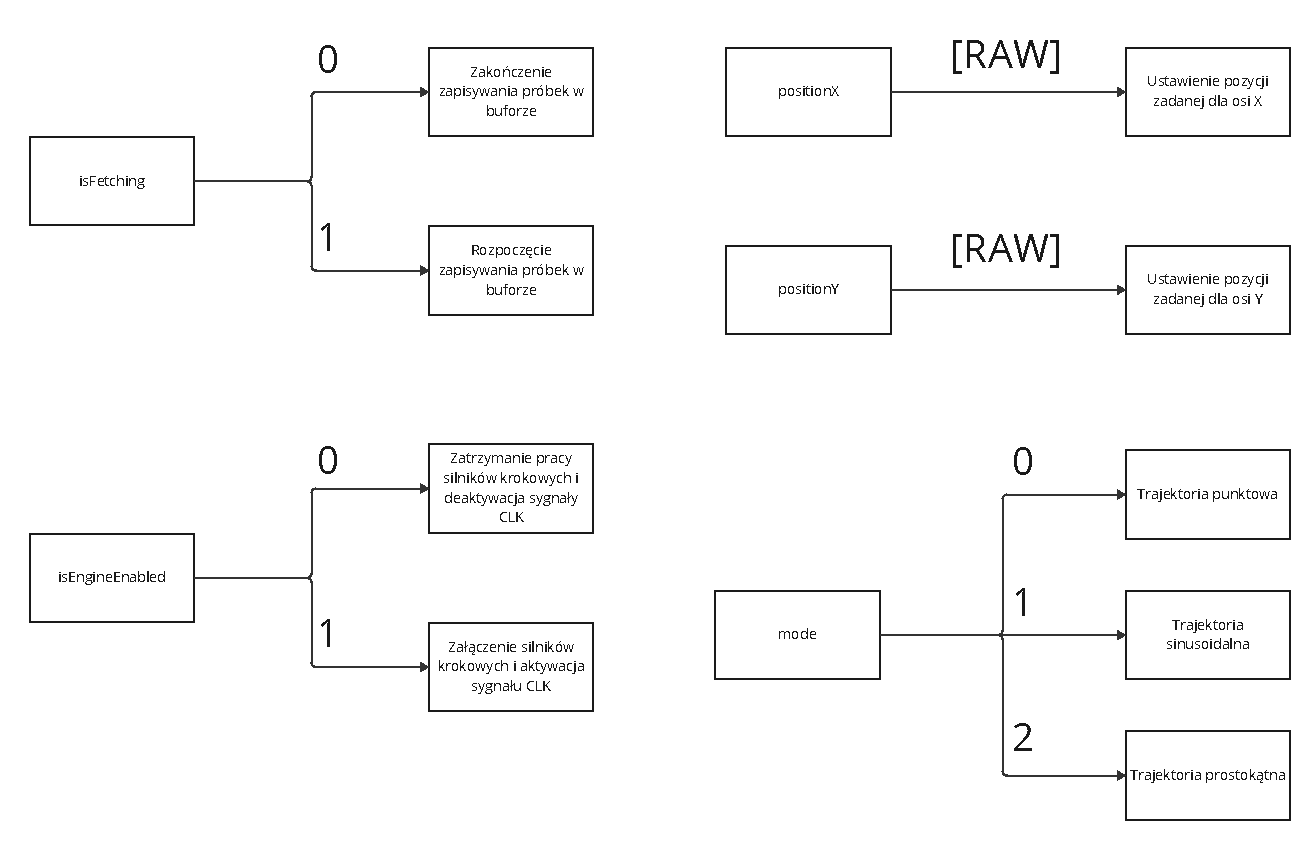
\includegraphics{interface/schemat blokowy json webowa.pdf}}
    \caption{Schemat blokowy struktury JSON z aplikacji webowej.}
    \label{fig:schemat blokowy komunikacji z aplikacji webowej do serwera na STM32}
\end{figure}

W trakcie przesyłania wiadomości nie trzeba przesyłać wszystkich kluczy z wartościami, serwer na STM32 przetworzy tylko wysłane dane. Jest to przydatne w celu zmniejszenia rozmiaru wiadomości oraz ograniczenia błędów w przypadku nie wysłania kluczy ze wszystkimi wartościami. \\
String przesyłany z aplikacji webowej jest na tyle mały, że nie trzeba rozważać przesyłania jednej wiadomości w paru fragmentach (ang. \textit{chunks}).

\section{Komunikacja z STM32 do aplikacji webowej}
Do komunikacji z STM32 do aplikacji webowej również został wybrany format danych typu \textbf{JSON}. Przykład komunikacji został przedstawiony na schemacie
blokowym \ref{fig:schemat blokowy odpowiedzi serwera na STM32}.
\begin{lstlisting}[caption=Przykład struktury JSON z STM32 do aplikacji webowej, label={lst:json_exampleSTM32}]
{
  "dataX": [int],
  "dataY": [int],
  "dataErrorX": [int],
  "dataErrorY": [int]
}
\end{lstlisting}
\begin{enumerate}
    \item \textbf{dataX:} Odczytane próbki z osi X w formacie RAW.
    \item \textbf{dataY:} Odczytane próbki z osi Y w formacie RAW.
    \item \textbf{dataErrorX:} Uchyb na osi X w formacie RAW.
    \item \textbf{dataErrorY:} Uchyb na osi Y w formacie RAW.
\end{enumerate}

\begin{figure}[H]
    \centering
    \resizebox{6cm}{!}{
    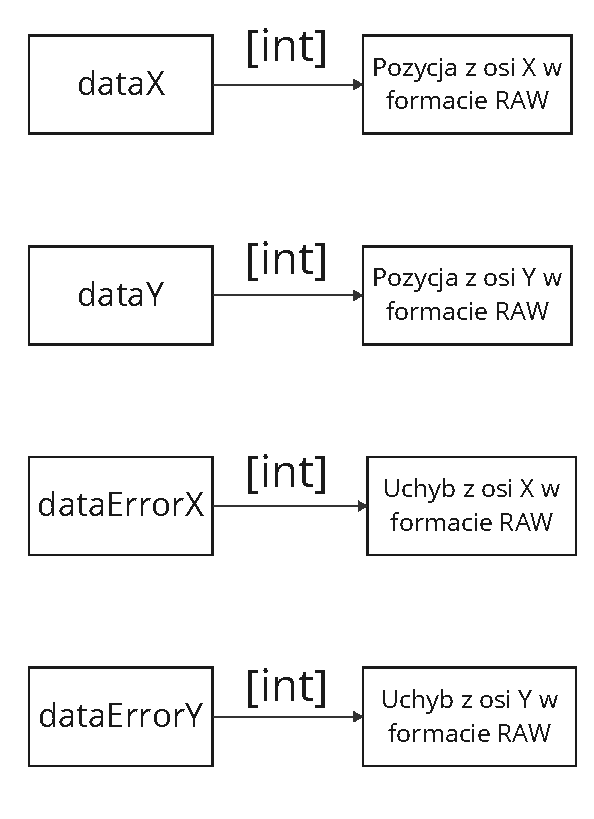
\includegraphics{interface/schemat blokowy json stm32.pdf}}
    \caption{Schemat blokowy odpowiedzi struktury JSON z serwera na STM32.}
  \label{fig:schemat blokowy odpowiedzi serwera na STM32}
\end{figure}
Aby przekształcić wartość z enkodera wyrażoną w jednostkach RAW na stopnie kątowe, należy pomnożyć ją przez 3.428374026619764e-7.  
W celu uzyskania radianów wartość RAW należy pomnożyć przez 5.98364147543706e-9.\\
Przesyłany ciąg znaków może być na tyle duży, że wiadomość zostanie podzielona na dwie lub więcej części. W związku z tym konieczne jest buforowanie fragmentów, ich łączenie oraz sprawdzanie, czy cała wiadomość została już odebrana. Ciąg znaków zawsze kończy się znakiem "\textbf{\}}", co ułatwia identyfikację końca wiadomości i umożliwia poprawne łączenie fragmentów.

% \chapter{WebSocket}
%  WebSocket \cite{WebSocket} to protokół komunikacyjny, który umożliwia dwukierunkową komunikację w czasie rzeczywistym pomiędzy serwerem, a klientem. Ów protokół jest jest szczególnie przydatny do komunikacji w aplikacjach sieciowych, które potrzebują dynamiczną wymianę danych w czasie rzeczywistym.
\section{Działanie WebSocket}
Protokół WebSocket rozpoczyna swoją pracę od \textit{handshake HTTP}. Klient inicjuje połączenie z WebSocketem wysyłając specjalne żądanie HTTP do serwera. Serwer otrzymuje to żądanie, a następnie decyduje czy chce je zaakceptować, następnie wysyła odpowiedź HTTP. Jeżeli zaakceptował żądanie to przy odpowiedzi ustawia trwałe połączenie. Po nawiązaniu połączenia obydwie strony mogą przesyłać dane bez potrzebny ponownego połączenia.

\section{Zalety WebSocket}
WebSocket posiada wiele zalety w stosunku do innych tradycyjnych protokołów komunikacyjnych. Porównano zalety nad protokołem HTTP:
\begin{enumerate}
    \item \textbf{Dwukierunkowa komunikacja w czasie rzeczywistym:} dane mogą być przesyłane w obu kierunkach. Protokół HTTP umożliwia tylko zapytanie do serwera i odpowiedź z jego strony. Jest to przydatne w przypadku asynchronicznych zdarzeń wymagających komunikacji. Dodatkowo redukuje to opóźnienia.
    \item \textbf{Stałe połączenie:} po nawiązaniu połączenia nie trzeba ponownie tego robić, co znacząco zmniejsza zmniejsza opóźnienia i zużycie zasobów.
    \item \textbf{Mniejsze zużycie pasma:} WebSocket pozwala na przesyłanie czystych danych bez nagłówków HTTP, co znacząco redukuje ilość przesyłanych danych.
\end{enumerate}

% \chapter{Aplikacja webowa}
% \begin{figure}[!htb]
    \centering
    \resizebox{15.5cm}{!}{
    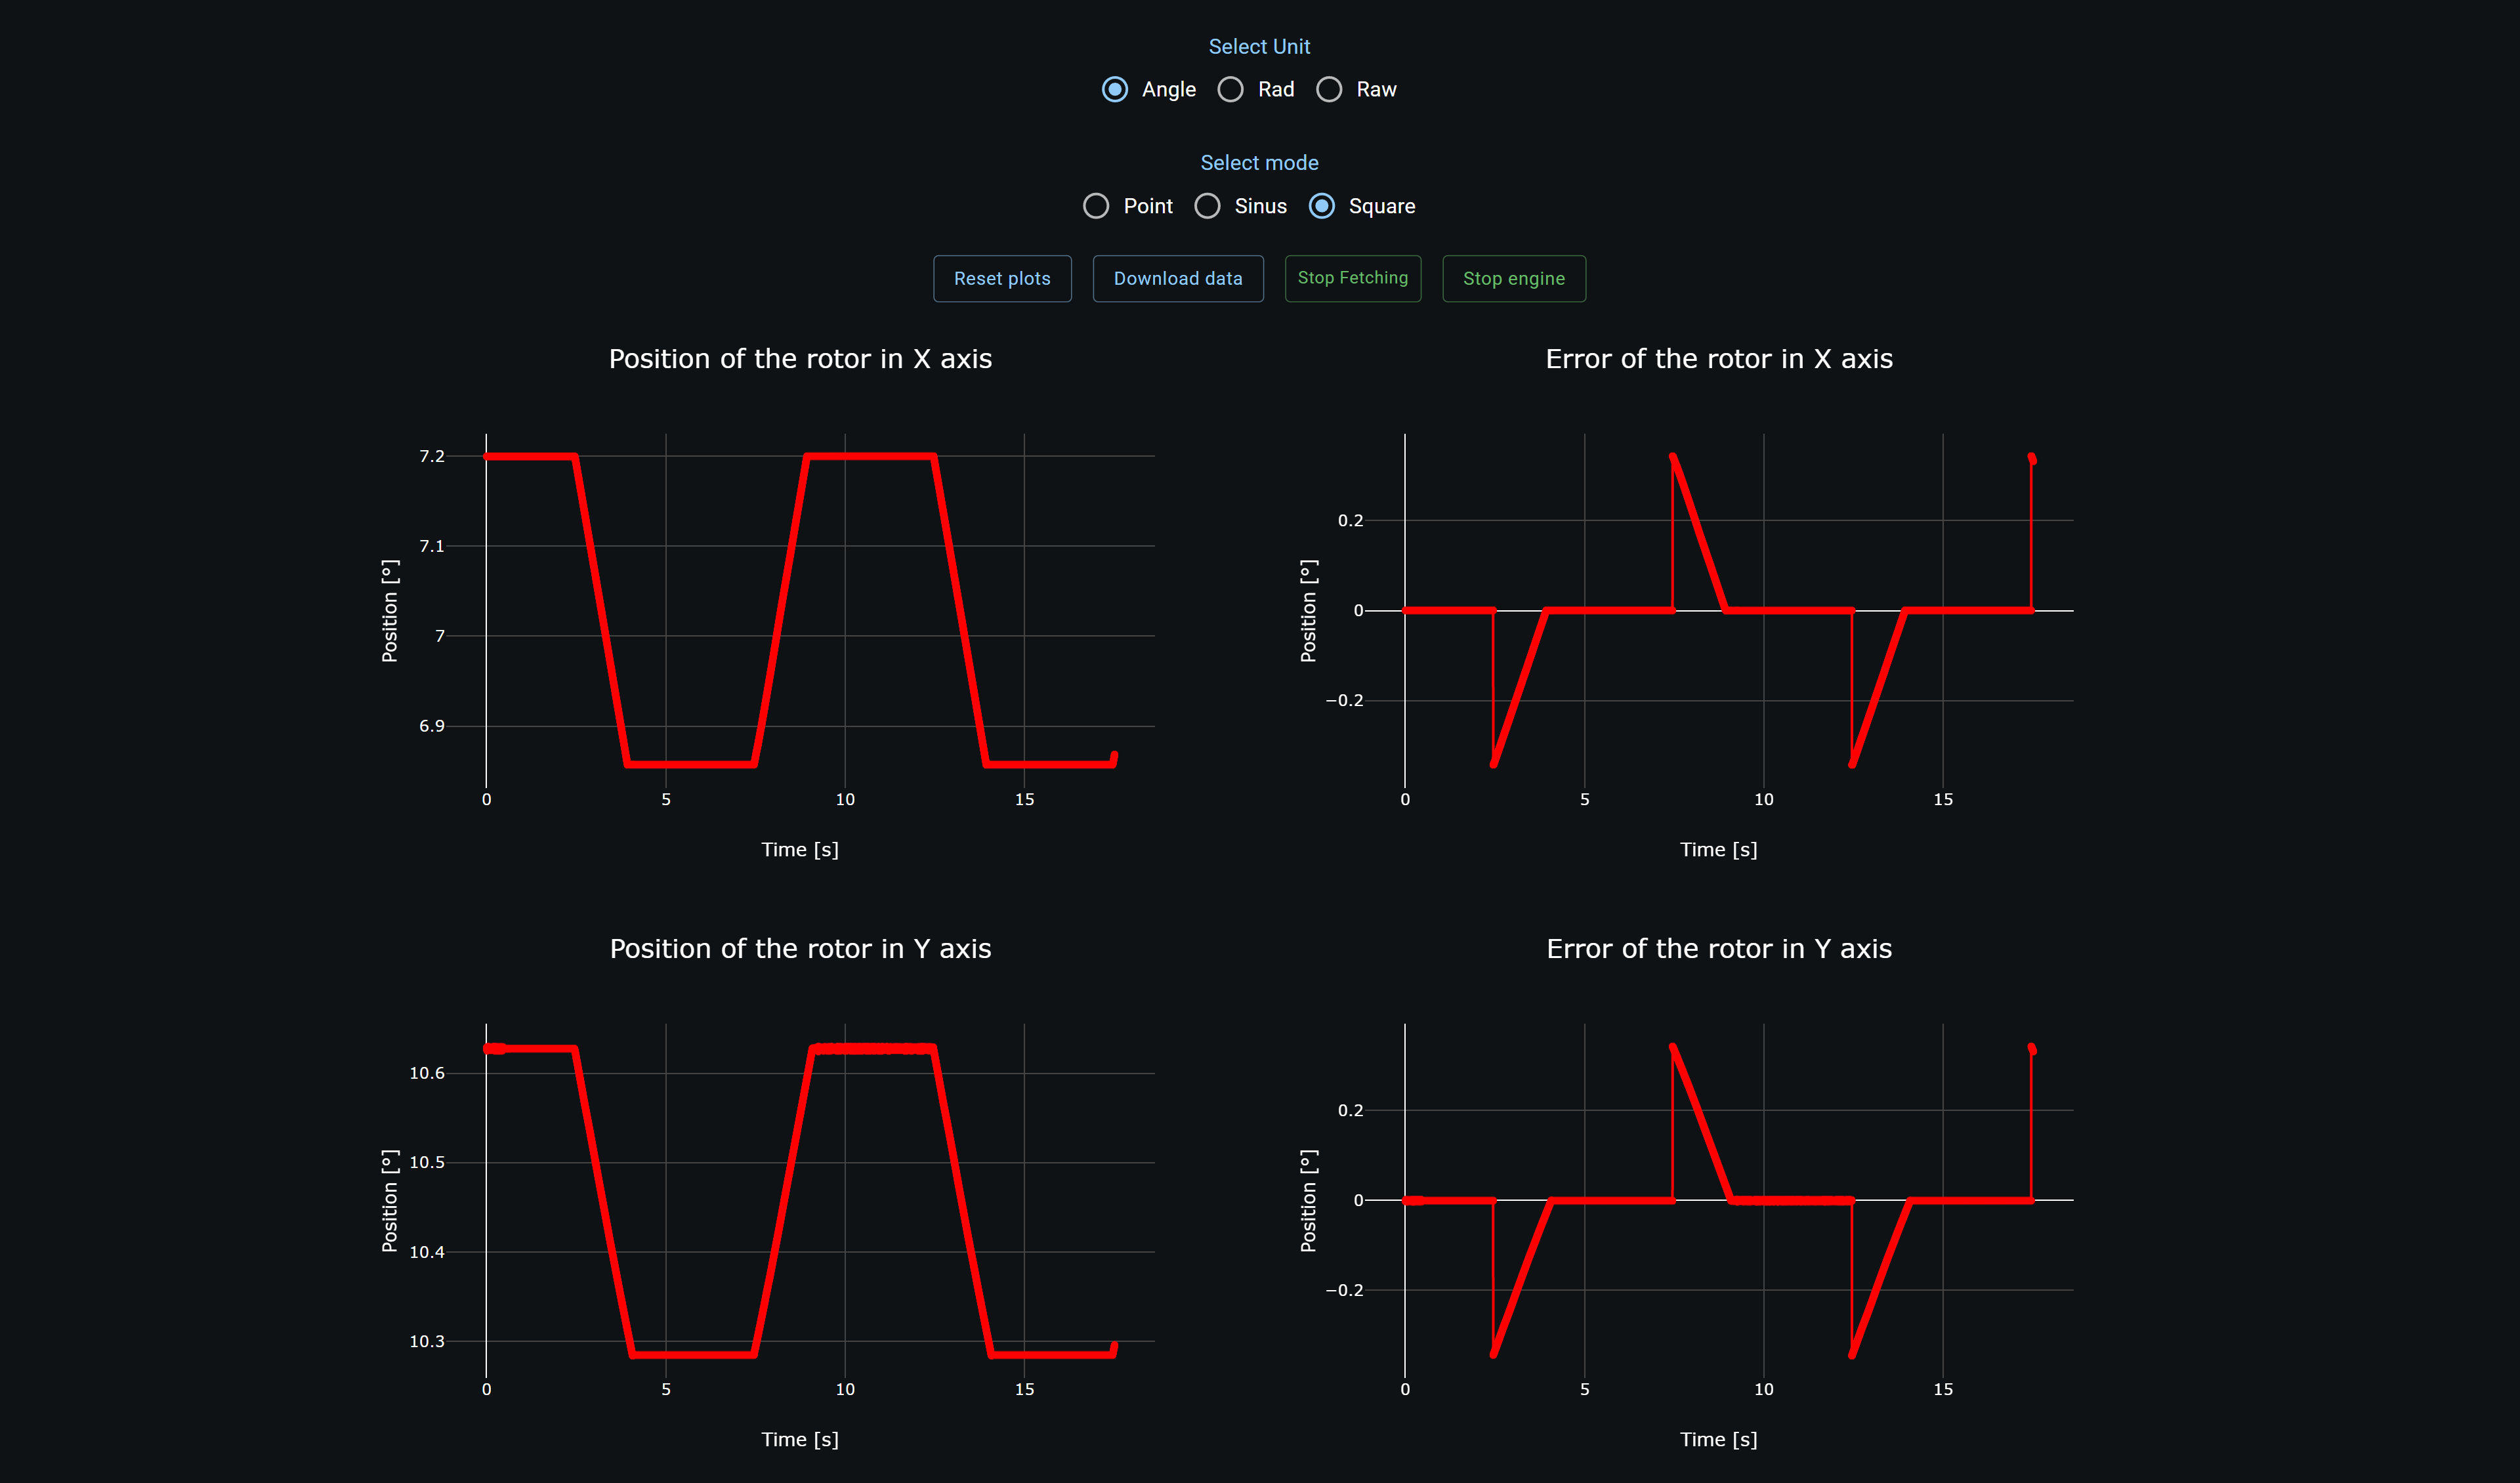
\includegraphics{interface/aplikacja webowa.png}}
    \label{fig:Interfejs}
    \caption{Interfejs użytkownika}
\end{figure}
\section{Funkcja wyboru jednostki}
\begin{enumerate}
    \item \textbf{Angle:} pozycja w stopniach.
    \item \textbf{Rad:} pozycja w radianach.
    \item \textbf{Raw:} pozycja odczytana przez enkoder.
\end{enumerate}
Wybranie jednostki powoduje zmianę wartości na osi rzędnych wykresów. Dodatkowo podczas wpisywania pozycji brana jest wybrana jednostka np. przy wybraniu \textbf{Raw} wpisujemy wartość np. \textit{20000000}, natomiast przy wybraniu \textbf{Rad} wpisujemy np. \textit{0.12} w celu ustawienia pozycji.
\section{Wybranie trybu wartości zadanej}
\begin{enumerate}
    \item \textbf{Point:} pokazuje interfejs z polami tekstowymi, które umożliwiają wpisanie wartości zadanej.
    \item \textbf{Sinus:} ustawia trajektorie sinusoidalną.
    \item \textbf{Square:} ustawia trajektorie prostokątną.
\end{enumerate}
W przypadku wybrania trybu \textbf{Sinus} lub \textbf{Square} interfejs z inputami do wpisywania wartości zadanej jak i przycisk \textbf{Send message} jest chowany.
\section{Przyciski funkcyjne}
\begin{enumerate}
    \item \textbf{Reset plots:} usuwa aktualne próbki w pamięci, również czyści wykresy.
    \item \textbf{Download data:} pobiera aktualne próbki w formacie JSON, struktura jest taka sama jak JSON przesyłany z STM32 do aplikacji webowej.
    \item \textbf{Start Fetching:} aktywuje pobieranie próbek do buforu na STM32. Załącza zegar, który co \textit{200ms} pobiera próbki z STM32 próbki i wyświetlane na wykresach. Po pobraniu próbek bufor na STM32 jest czyszczony. Dodatkowo zmienia nazwę przycisku na "Stop Fetching" i zmienia kolor na zielony.
    \item \textbf{Stop Fetching:} wyłącza zegar odpowiedzialny za pobieranie próbek co 200ms, a następnie zmienia nazwę przycisku na "Start Fetching" i zmienia kolor.
    \item \textbf{Start engine:} aktywuje piny pozwalające na pracę rotorów. Również aktywuje sygnał \textit{CLK} odpowiedzialny za ruch rotorów.
    \item \textbf{Send message:} wpisana pozycja jest przekształcana na jednostkę Raw, a następnie jest przesyłana do STM32. Końcowo STM32 ustawia te pozycje jako wartości zadane.
\end{enumerate}
W polach tekstowych Position X i Position Y należy wpisać wartość zadaną według wybranej jednostki.
\section{Schemat blokowy pobierania danych}
Po wciśnięciu przycisku \textit{Start Fetching} w interfejsie użytkownika załączany jest zegar z okresem \textit{200ms}. Rozpoczyna on cykliczny proces wymiany danych pomiędzy frontendem, backendem jak i mikrokontrolerem. Szczegółowy opis komunikacji:

\begin{enumerate}
    \item \textbf{Frontend:} inicjuje wysyłanie zapytań w formacie JSON do backendu za pomocą protokołu WebSocket. Każda wiadomość zawiera klucz \textbf{isFetching} o wartości \textit{1}. 
    \item \textbf{Backend:} przesyła otrzymaną wiadomość do serwera na mikrokontrolerze.
    \item \textbf{Serwer na mikrokontrolerze:}  Po otrzymaniu klucza \textbf{isFetching} o wartości \textit{1}, rozpoczyna się zapisywanie próbek z aktualną pozycją i uchybem do bufora, o ile zapis nie był wcześniej zainicjowany. Po przetworzeniu danych z backendu, serwer zwraca JSON'a o strukturze zawartej w listingu \ref{lst:json_exampleSTM32}. W przypadku pierwszego zapytania bufor jest pusty, dlatego serwer zacznie zwracać niepuste dane dopiero od drugiego zapytania. Po przesłaniu danych bufor z aktualną pozycją i uchybem jest czyszczony.
    \item \textbf{Powrót danych z serwera:} Backend otrzymuje wiadomość w fragmentach i składa ją w całość. Każdy fragment jest dodawany do buforu. W przypadku gdy cała wiadomość jest w buforze, czyli zawiera znak końca JSON "\textbf{\{}", wysyła ją do frontendu za pomocą protokołu WebSocket, a po jej wysłaniu usuwa ją z buforu. W przypadku braku pełnej wiadomości backend oczekuje na kolejne fragmenty. Frontend, po otrzymaniu wiadomości, aktualizuje wykresy, dodając nowe próbki o aktualnej pozycji i uchybie.
    \item \textbf{Zatrzymanie procesu:} Proces powtarza się co \textit{200ms}, dopóki użytkownik nie naciśnie przycisku \textit{Stop Fetching}. Po jego aktywacji zegar zostanie zatrzymany i zostanie wysłana wiadomość z kluczem \textit{isFetching} o wartości \textit{0}, co skutkuje zatrzymaniem zapisywania aktualnych próbek do buforu na mikrokontolerze.
\end{enumerate}
Na Rys. ~\ref{fig:schemat blokowy pobierania danych} przedstawiono proces wymiany danych między frontendem, backendem aplikacji webowej i serwerem na mikrokontrolerze.
 \begin{figure}[H]
    \centering
    \resizebox{15.5cm}{!}{
    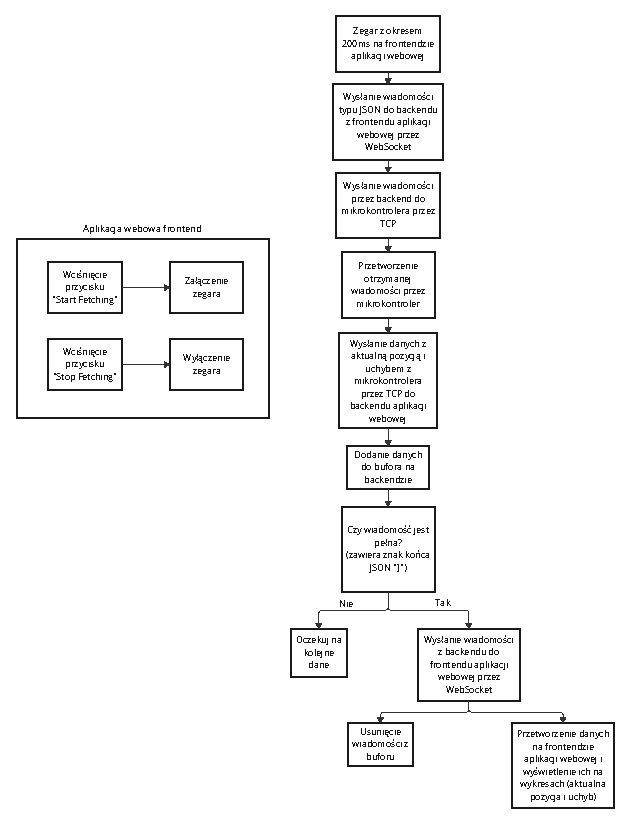
\includegraphics{interface/schemat blokowy pobierania danych.pdf}}
    \caption{Schemat blokowy pobierania pozycji i uchybu.}
    \label{fig:schemat blokowy pobierania danych}
\end{figure}
\section{Docker}
Docker \cite{Docker} jest narzędziem do konteneryzacji, które umożliwia tworzenie i uruchamianie aplikacji w kontenerach, czyli odizolowanych środowiskach. Kontenery są instancjami obrazów Dockera, które dzięki swojej zoptymalizowanej budowie cechują się lekkością i możliwością ponownego wykorzystania. Zawierają jedynie niezbędne elementy do prawidłowego działania aplikacji.
\subsection{Działanie Dockera}
Docker polega na zasadzie wirtualizacji na poziomie systemu operacyjnego. Główne narzędzia Dockera:
\begin{enumerate}
    \item \textbf{Obrazy}: są to szablony zawierające system operacyjny i podstawowe zależności do działania aplikacji.
    \item \textbf{Kontenery}:
    Obraz Dockera może zostać uruchomiony jako kontener, który działa w odizolowanym środowisku. Dzięki temu wszyscy mogą pracować w identycznych warunkach, co eliminuje potrzebę tworzenia i konfigurowania środowisk dla każdej osoby z osobna. Ponadto Docker rozwiązuje problem różnic w działaniu aplikacji na różnych systemach operacyjnych, zapewniając spójność i przewidywalność.
\end{enumerate}

\subsection{Zalety Dockera}
\begin{enumerate}
    \item \textbf{Przenośność}: Kontenery mogą być uruchamiane na różnych systemach operacyjnych i infrastrukturach, co ułatwia wdrażanie aplikacji.
    Docker może zostać użyty na głównych systemach operacyjnych, co znacząco ułatwia wdrażanie aplikacji. Mac i linux posiadają paczki do instalacji dockera, natomiast na windowsie można użyć aplikacji docker deskop i dodatkowo zainstalować podsystem linux WSL2 (Windows subsystem for linux), w celu zwiększenia wydajności kontenerów.
    \item \textbf{Izolacja}:
    Aplikacja działa w odizolowanym środowisku, co minimalizuje konflikty między środowiskami i zależnościami.
    \item \textbf{Szybkość}:
    Kontenery są lekkie i szybkie do uruchomienia w porównaniu do maszyn wirtualnych. Kontenery używają tylko najpotrzebniejszych zależności, co przyczynia się do ich lekkości.
    \item \textbf{Skalowalność}: Docker umożliwia w prosty sposób skalowanie aplikacji, poprzez uruchamianie wielu kontenerów jednocześnie. Np. na jednym kontenerze mamy aplikację webową, a na drugim można byłoby dodać bazę danych.
\end{enumerate}
\subsection{Obraz i kontener użyty w aplikacji}
Przy budowaniu obrazu został rozszerzony obraz \textit{node:22-alpine}, \textit{alpine} oznacza okrojoną wersję, która posiada tylko najpotrzebniejsze zależności. Na tym obrazie dostępny jest Node.js w wersji 22. Dodatkowo został zainstalowany bash, który ułatwia poruszanie się po zbudowanym kontenerze. Do zbudowania obrazu zostały użyte polecenia instalujące paczki NPM potrzebne do prawidłowego działania aplikacji, dodatkowo instalowana jest globalnie paczka serve, która służy do obsługi serwera HTTP. Po włączeniu kontenera inicjowane są polecenia uruchamiające WebSocket na porcie \textbf{8080} jak i aplikacje webową, przy użyciu serwera HTTP, na porcie \textbf{3000}. Powyższe porty są udostępniane kontenerowi za pomocą polecenia \textit{EXPOSE}. W pliku konfiguracyjnym kontenera zdefiniowano również porty hosta, które są dostępne z poziomu komputera. Porty hosta mogą być takie same jak w kontenerze, ale istnieje możliwość ich zmiany, co pozwala na mapowanie różnych portów na potrzeby specyficznych konfiguracji i unikanie konfliktów. Nazwa kontenera została ustawiona na app\_container. Dodatkowo została udostępniona sieć dla kontenera, w celu prawidłowego połączenia się z serwerem na STM32.
\subsection{Uruchomienie aplikacji w kontenerze}
Całą aplikację można uruchomić poleceniem \textit{docker compose up}. Po użyciu tej komendy na porcie \textbf{3000} jest dostępna aplikacja z intefejsem do obsługi teleskopu i WebSocket na porcie \textbf{8080}. W celu wejścia na kontener należy użyć polecenia \textit{docker exec -it app\_container bash}.

% \chapter{Testy}
% \indent W celu sprawdzenia poprawności działania stanowiska zrealizowano różne testy eksperymentalne. Przeprowadzono ocenę wpływu zakłóceń w postaci impulsów siły przykładanych w różnych punktach konstrukcji na dokładność utrzymania zadanego położenia oraz zbadano jakość odtwarzania pozycji w poszczególnych osiach. W czasie testów zbadano przebiegi sinusoidalne oraz prostokątne. Dla trajektorii sinusoidalnej zmieniano częstotliwość sinusa, co pozwoliło wyznaczyć wartość graniczną, przy której układ tracił zdolność nadążania. W dalszych etapach sprawdzono także podstawową wadę silników krokowych do tzw. gubienia kroków - zjawiska występującego przy zbyt dużych prędkościach nadawanych napędom. Również zilustrowano przebieg sygnałów określających kierunek obrotu silnika.

\begin{center}
    \textbf{Parametry eksperymentu}
\end{center}

\noindent Dla wszystkich sinusoidalnych i prostokątnych trajektorii zadanych określonych dla obu osi wartość amplitudy wynosiła 500000 RAW, czyli około 3.43 $^{\circ}$. Tabela \ref{tab:min_max} przedstawia minimum i maksimum dla rozważanych przebiegów. Parametr $\epsilon$ opisujący promień strefy nieczułości wynosił 1000 RAW, czyli około 1.23 sekund kątowych. Trajektorie były generowane przez mikrokontroler z częstotliwością 10 kHz. Częstotliwość próbkowania oraz sterowania wynosiła 2 kHz.

\begin{table}[H]
    \centering
    \begin{tabular}{|l|l|l|l|l|}
        \hline
        & minimum {[}RAW{]} & minimum {[}$^{\circ}${]} & maksimum {[}RAW{]} & maksimum {[}$^{\circ}${]} \\ \hline
        X & 20000000 & $\sim$ 6.86 & 21000000 & $\sim$ 7.2 \\ \hline
        Y & 30000000 & $\sim$ 10.29 & 31000000 & $\sim$ 10.63 \\ \hline
    \end{tabular}
    \caption{Minimum i maksimum dla wszystkich trajektorii.}
    \label{tab:min_max}
\end{table}
\section{Zakłócenia}

\begin{figure}[H]
    \centering
    \resizebox{12cm}{!}{
    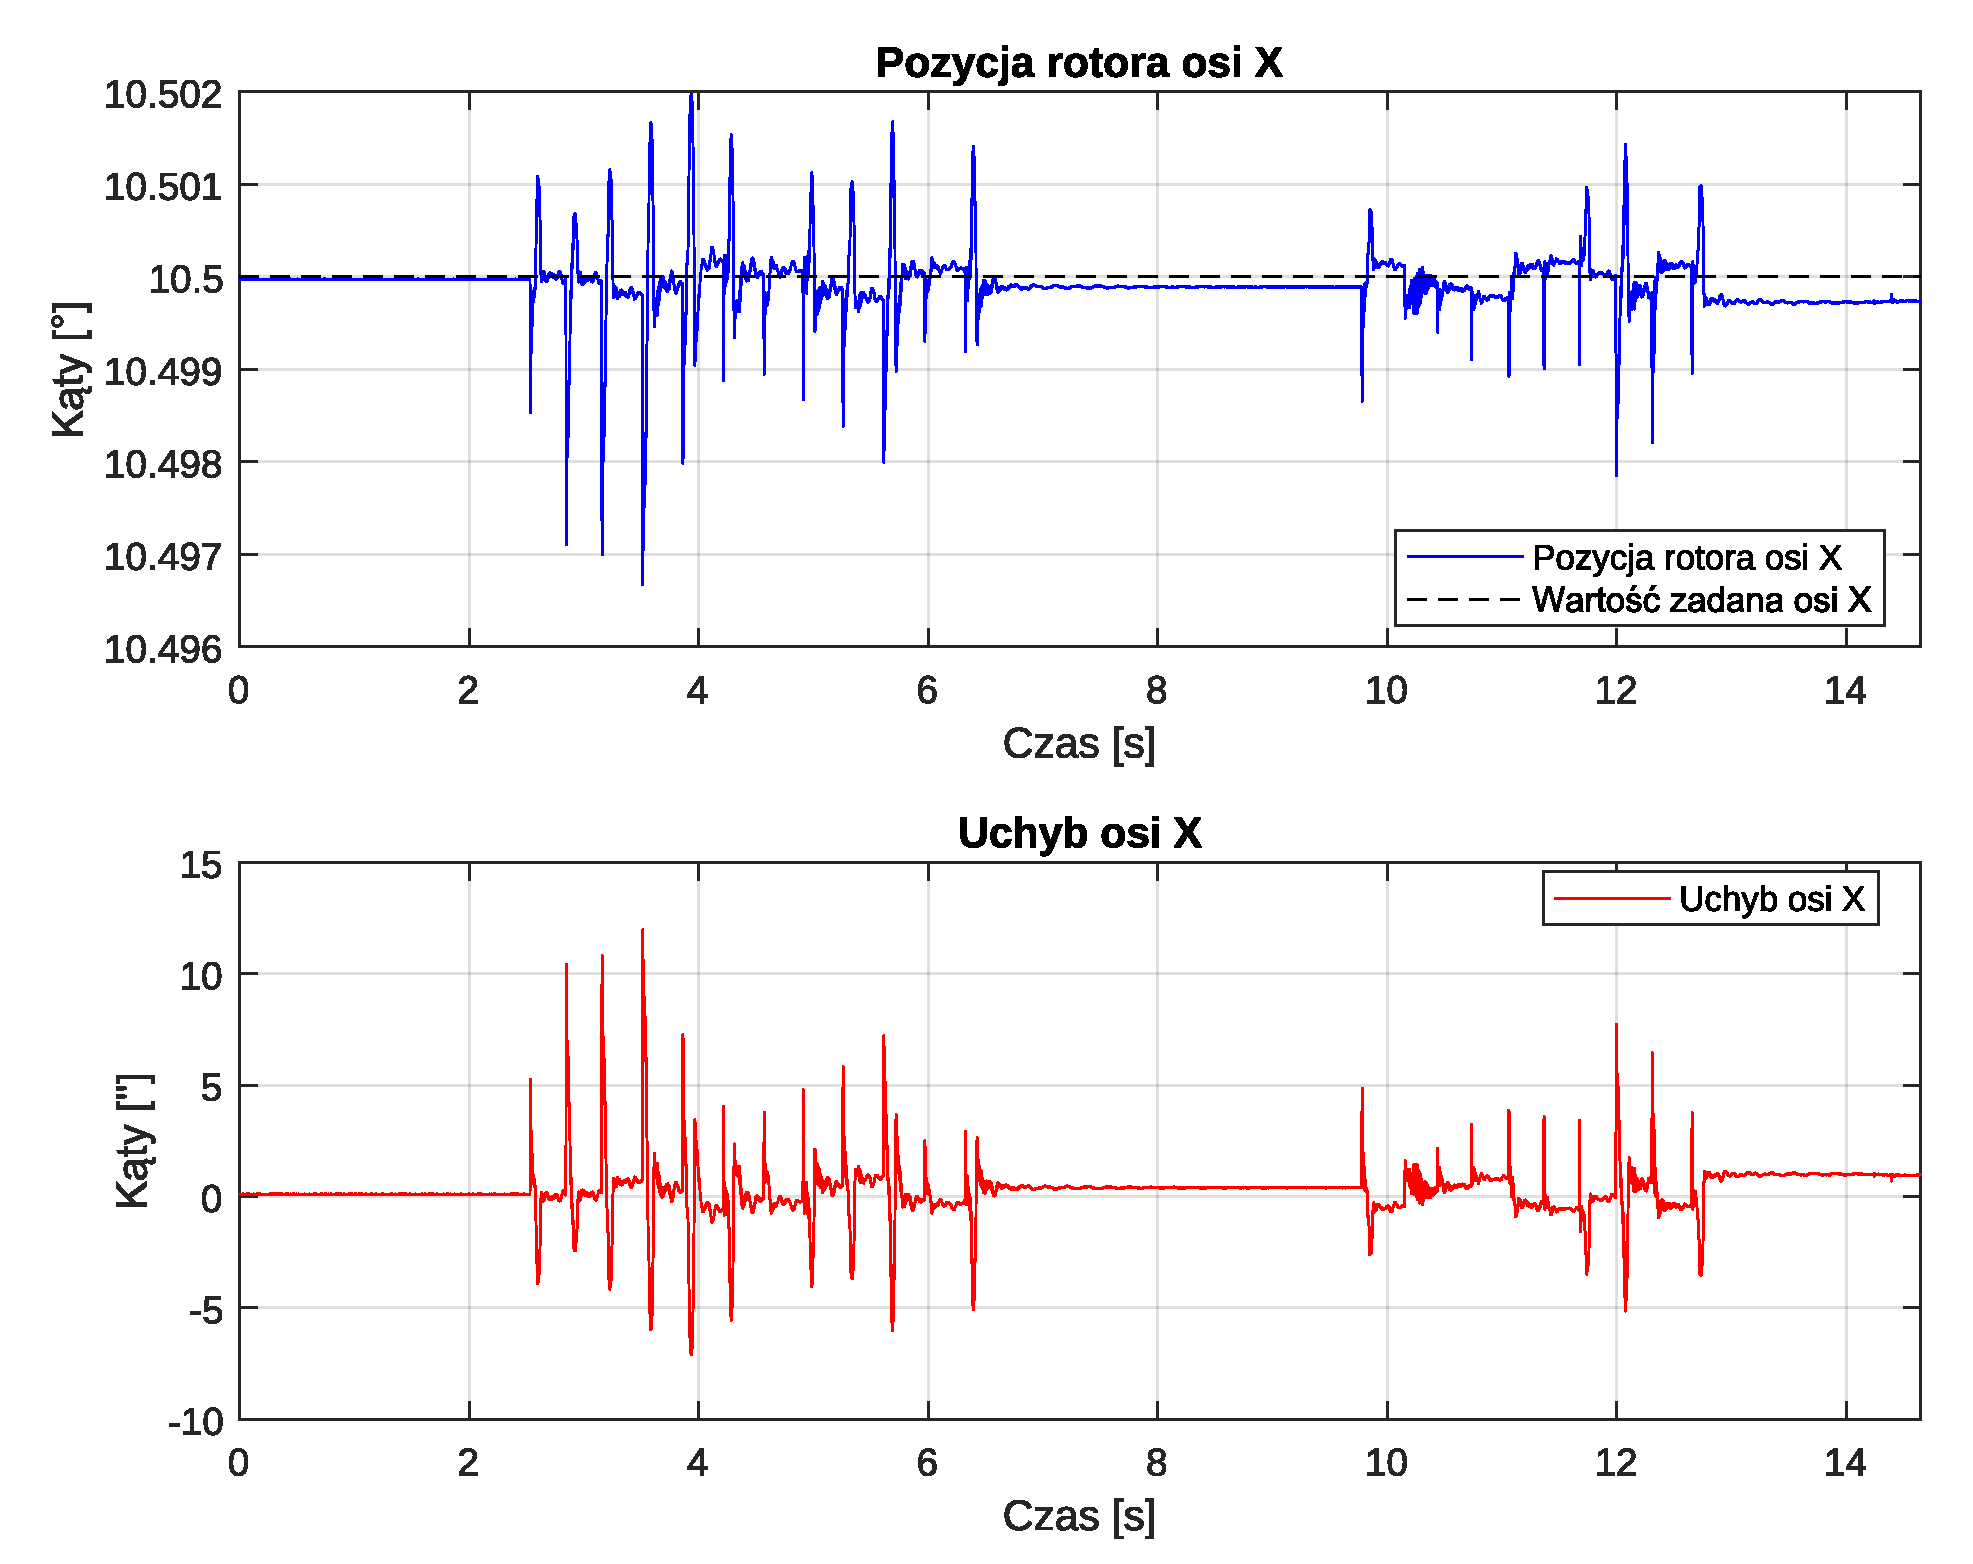
\includegraphics{testy/wykresy_inżynierka/pukanieX.pdf}}
    \caption{Przebiegi na osi X podczas zakłóceń mechanicznych.}
    \label{fig:schemat blokowy pobierania danych2}
\end{figure}

\begin{figure}[H]
    \centering
    \resizebox{12cm}{!}{
    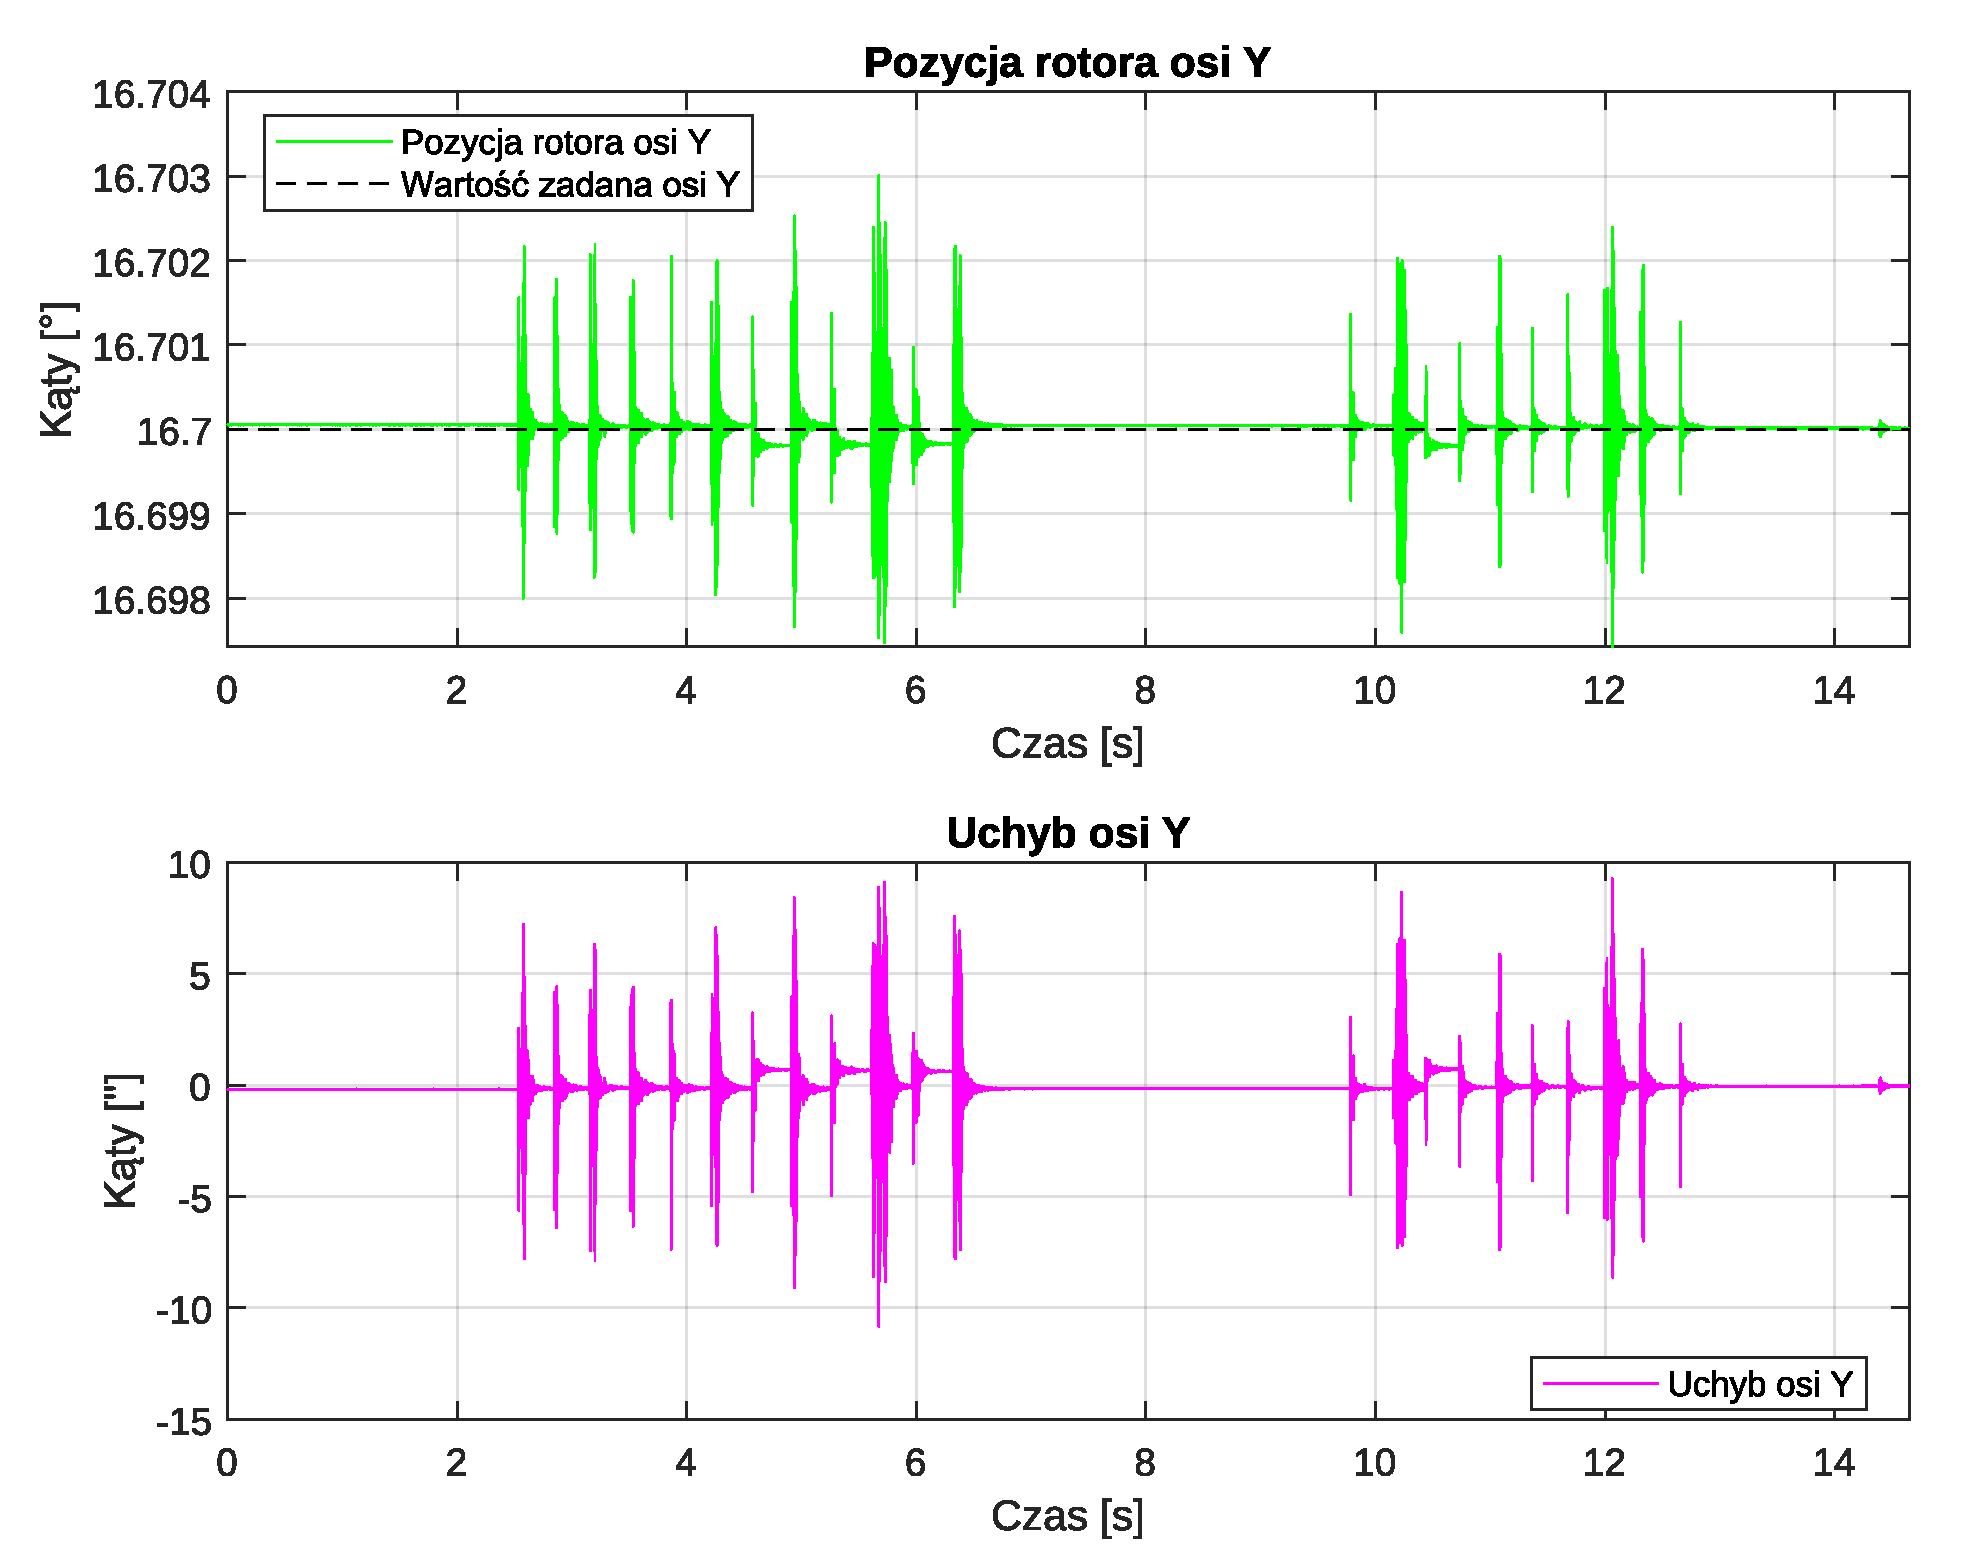
\includegraphics{testy/wykresy_inżynierka/pukanieY.pdf}}
    \caption{Przebiegi na osi Y podczas zakłóceń mechanicznych.}
    \label{fig:schemat blokowy pobierania danych2}
\end{figure}

\noindent Badano wpływ zakłócenia na jakość utrzymywania pozycji zadanej. Zakłócenia zostały wygenerowane przez delikatne uderzenia w konstrukcję w okolicach osi X. Wyniki pokazują występowanie drgań mechanicznych przenoszonych na całą konstrukcję. \newline
\noindent Po ustaniu tych drgań pozycja w obu osiach uległa niewielkiemu przesunięciu. Regulator nie przywraca pozycji zadanej, ponieważ wartość zarejestrowanego błędu położenia nie wykracza poza strefę nieczułości. Wprowadzenie tej strefy nieczułości było wymagane z uwagi na dyskretny charakter ruchu silnika krokowego oraz szumu pomiarowego pozycji.

\section{Trajektoria sinusoidalna}
W eksperymencie wykorzystano trajektorie sinusoidalne o różnych okresach takich jak: 1 s, 2 s, 5 s, 10 s i 200 s.

\begin{figure}[H]
    \centering
    \resizebox{12cm}{!}{
    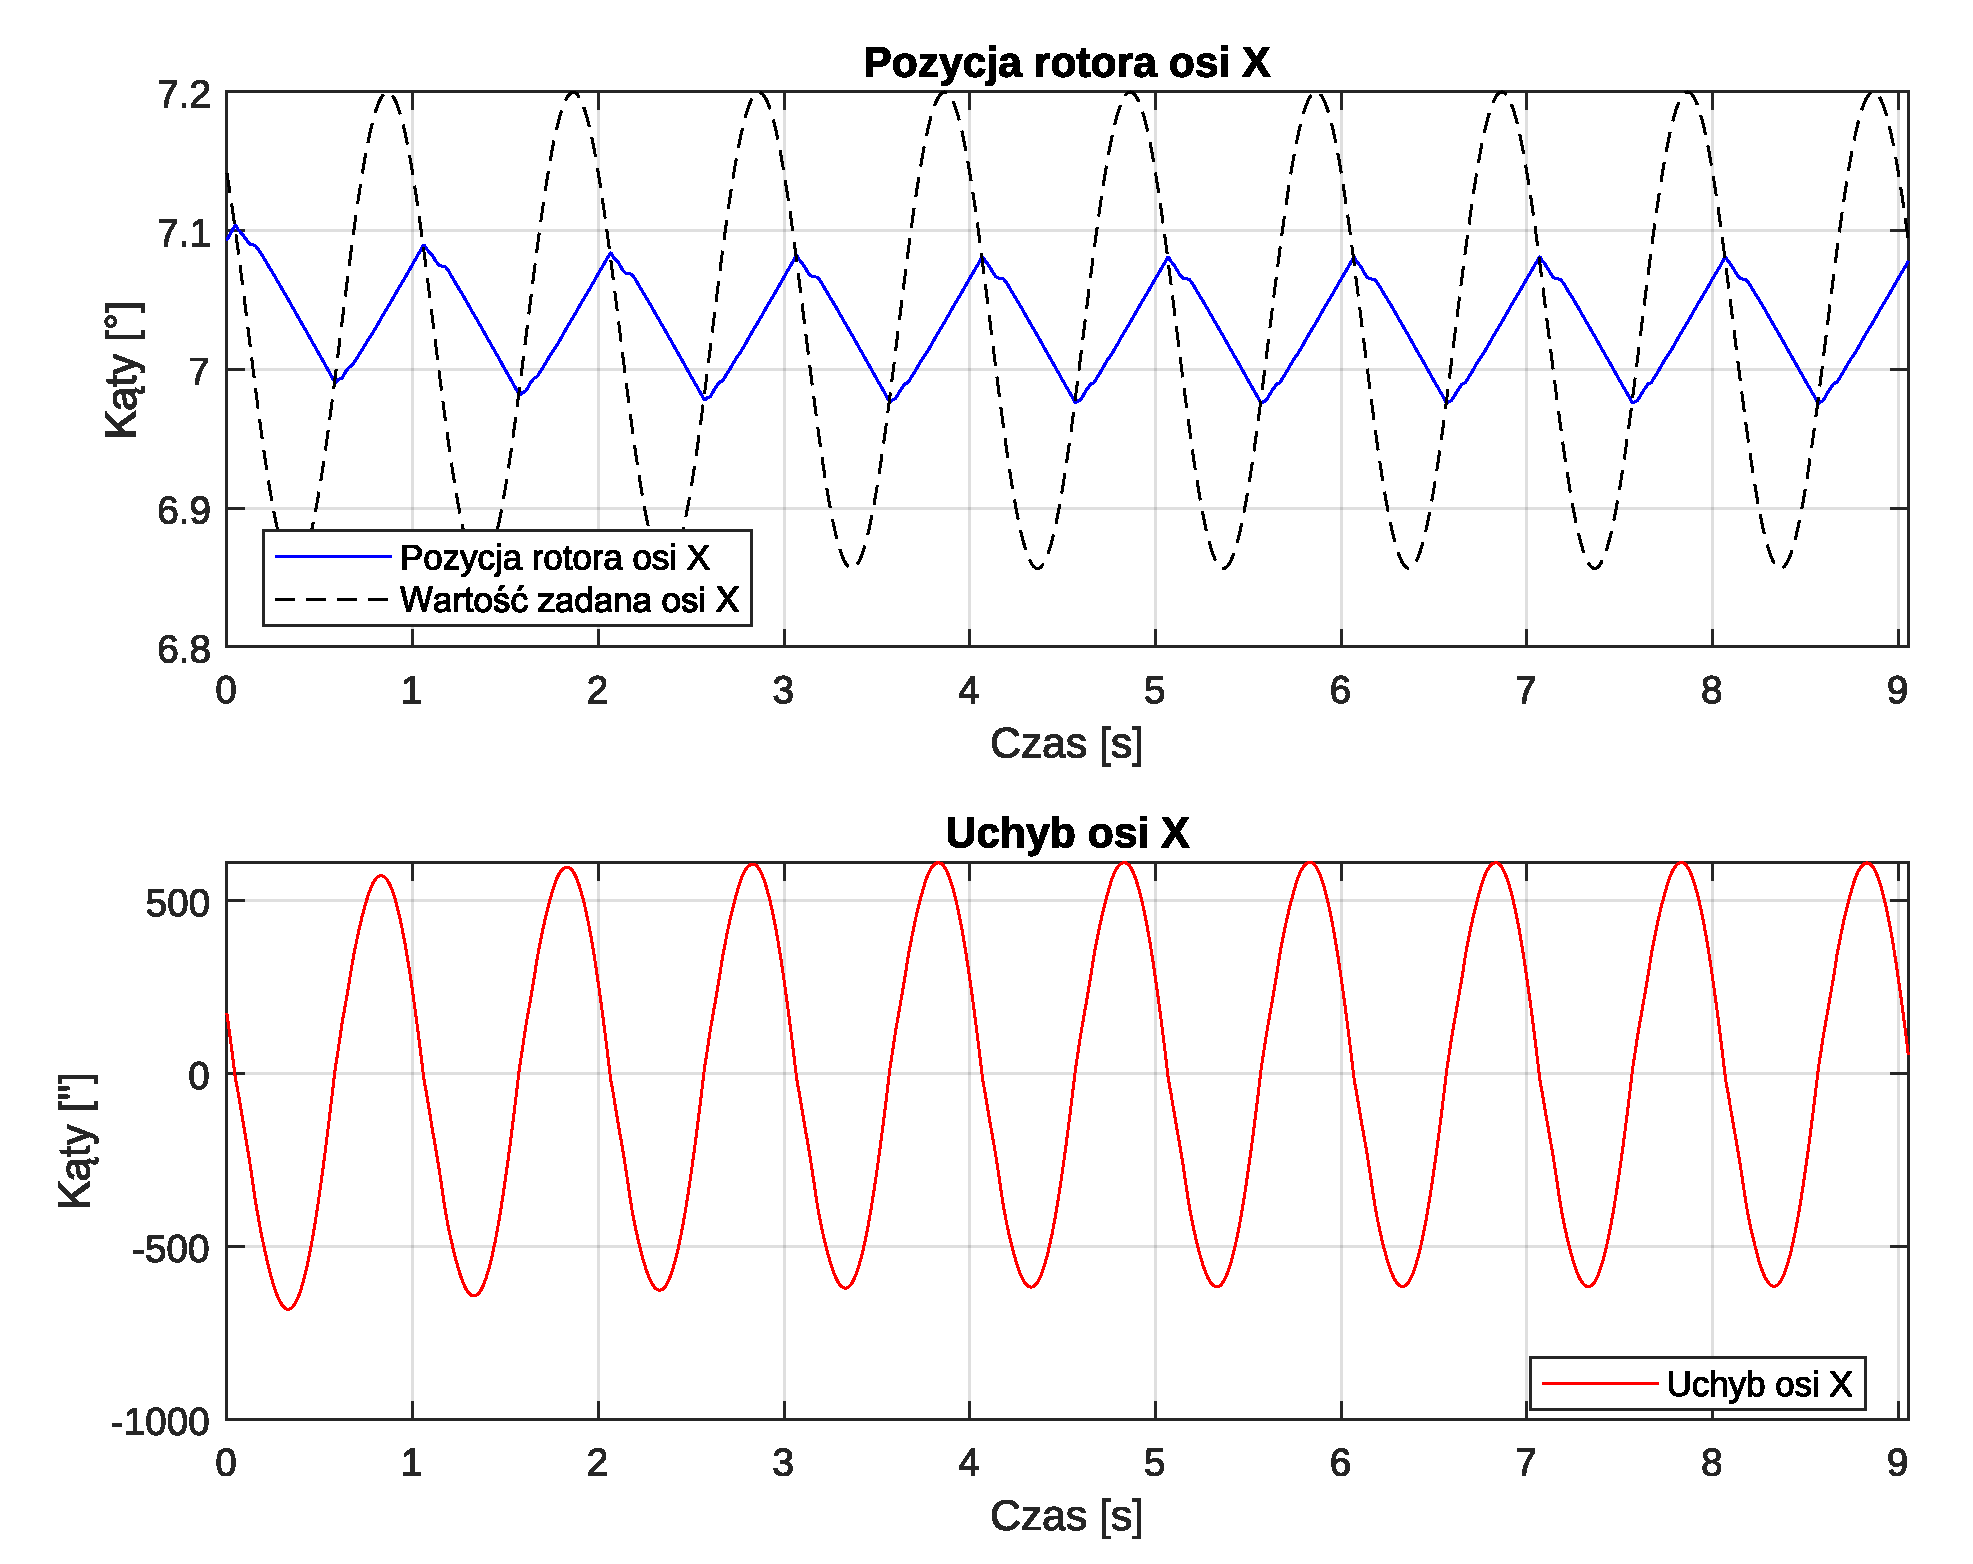
\includegraphics{testy/wykresy_inżynierka/sinus1sX.pdf}}
    \caption{Przebiegi dla trajektorii sinusoidalnej o okresie 1 sekund na osi X.}
    \label{fig:Przebiegi dla trajektorii sinusoidalnej o okresie 1 sekund na osi X.}
\end{figure}

\begin{figure}[H]
    \centering
    \resizebox{12cm}{!}{
    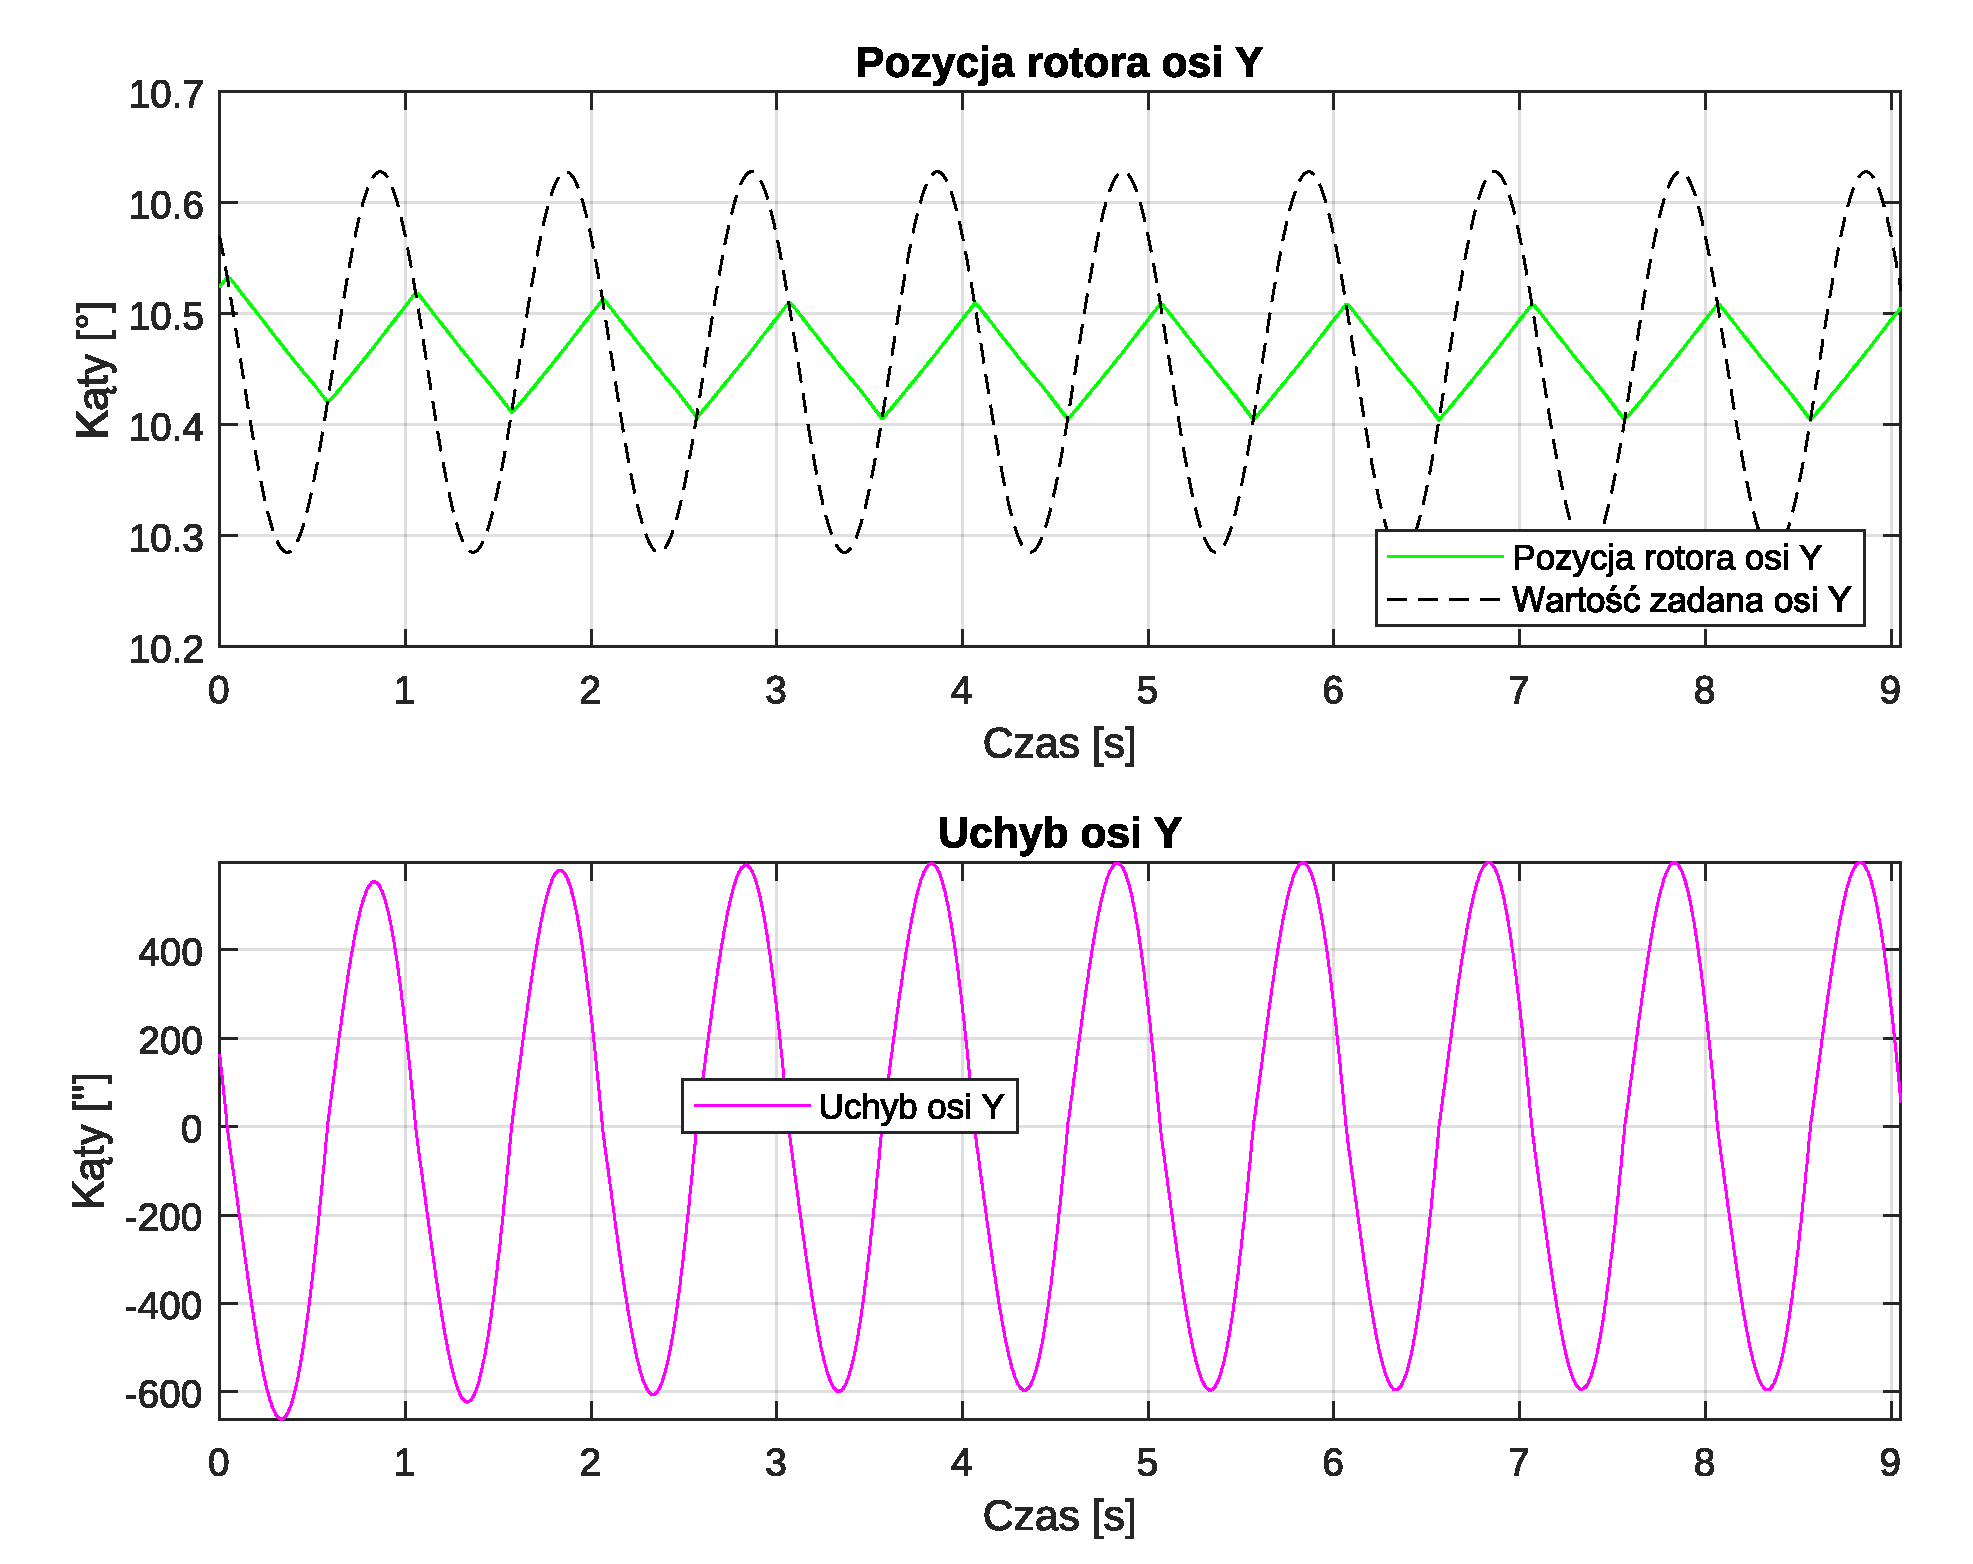
\includegraphics{testy/wykresy_inżynierka/sinus1sY.pdf}}
    \caption{Przebiegi dla trajektorii sinusoidalnej o okresie 1 sekund na osi Y.}
    \label{fig:Przebiegi dla trajektorii sinusoidalnej o okresie 1 sekund na osi Y.}
\end{figure}

\begin{figure}[H]
    \centering
    \resizebox{12cm}{!}{
    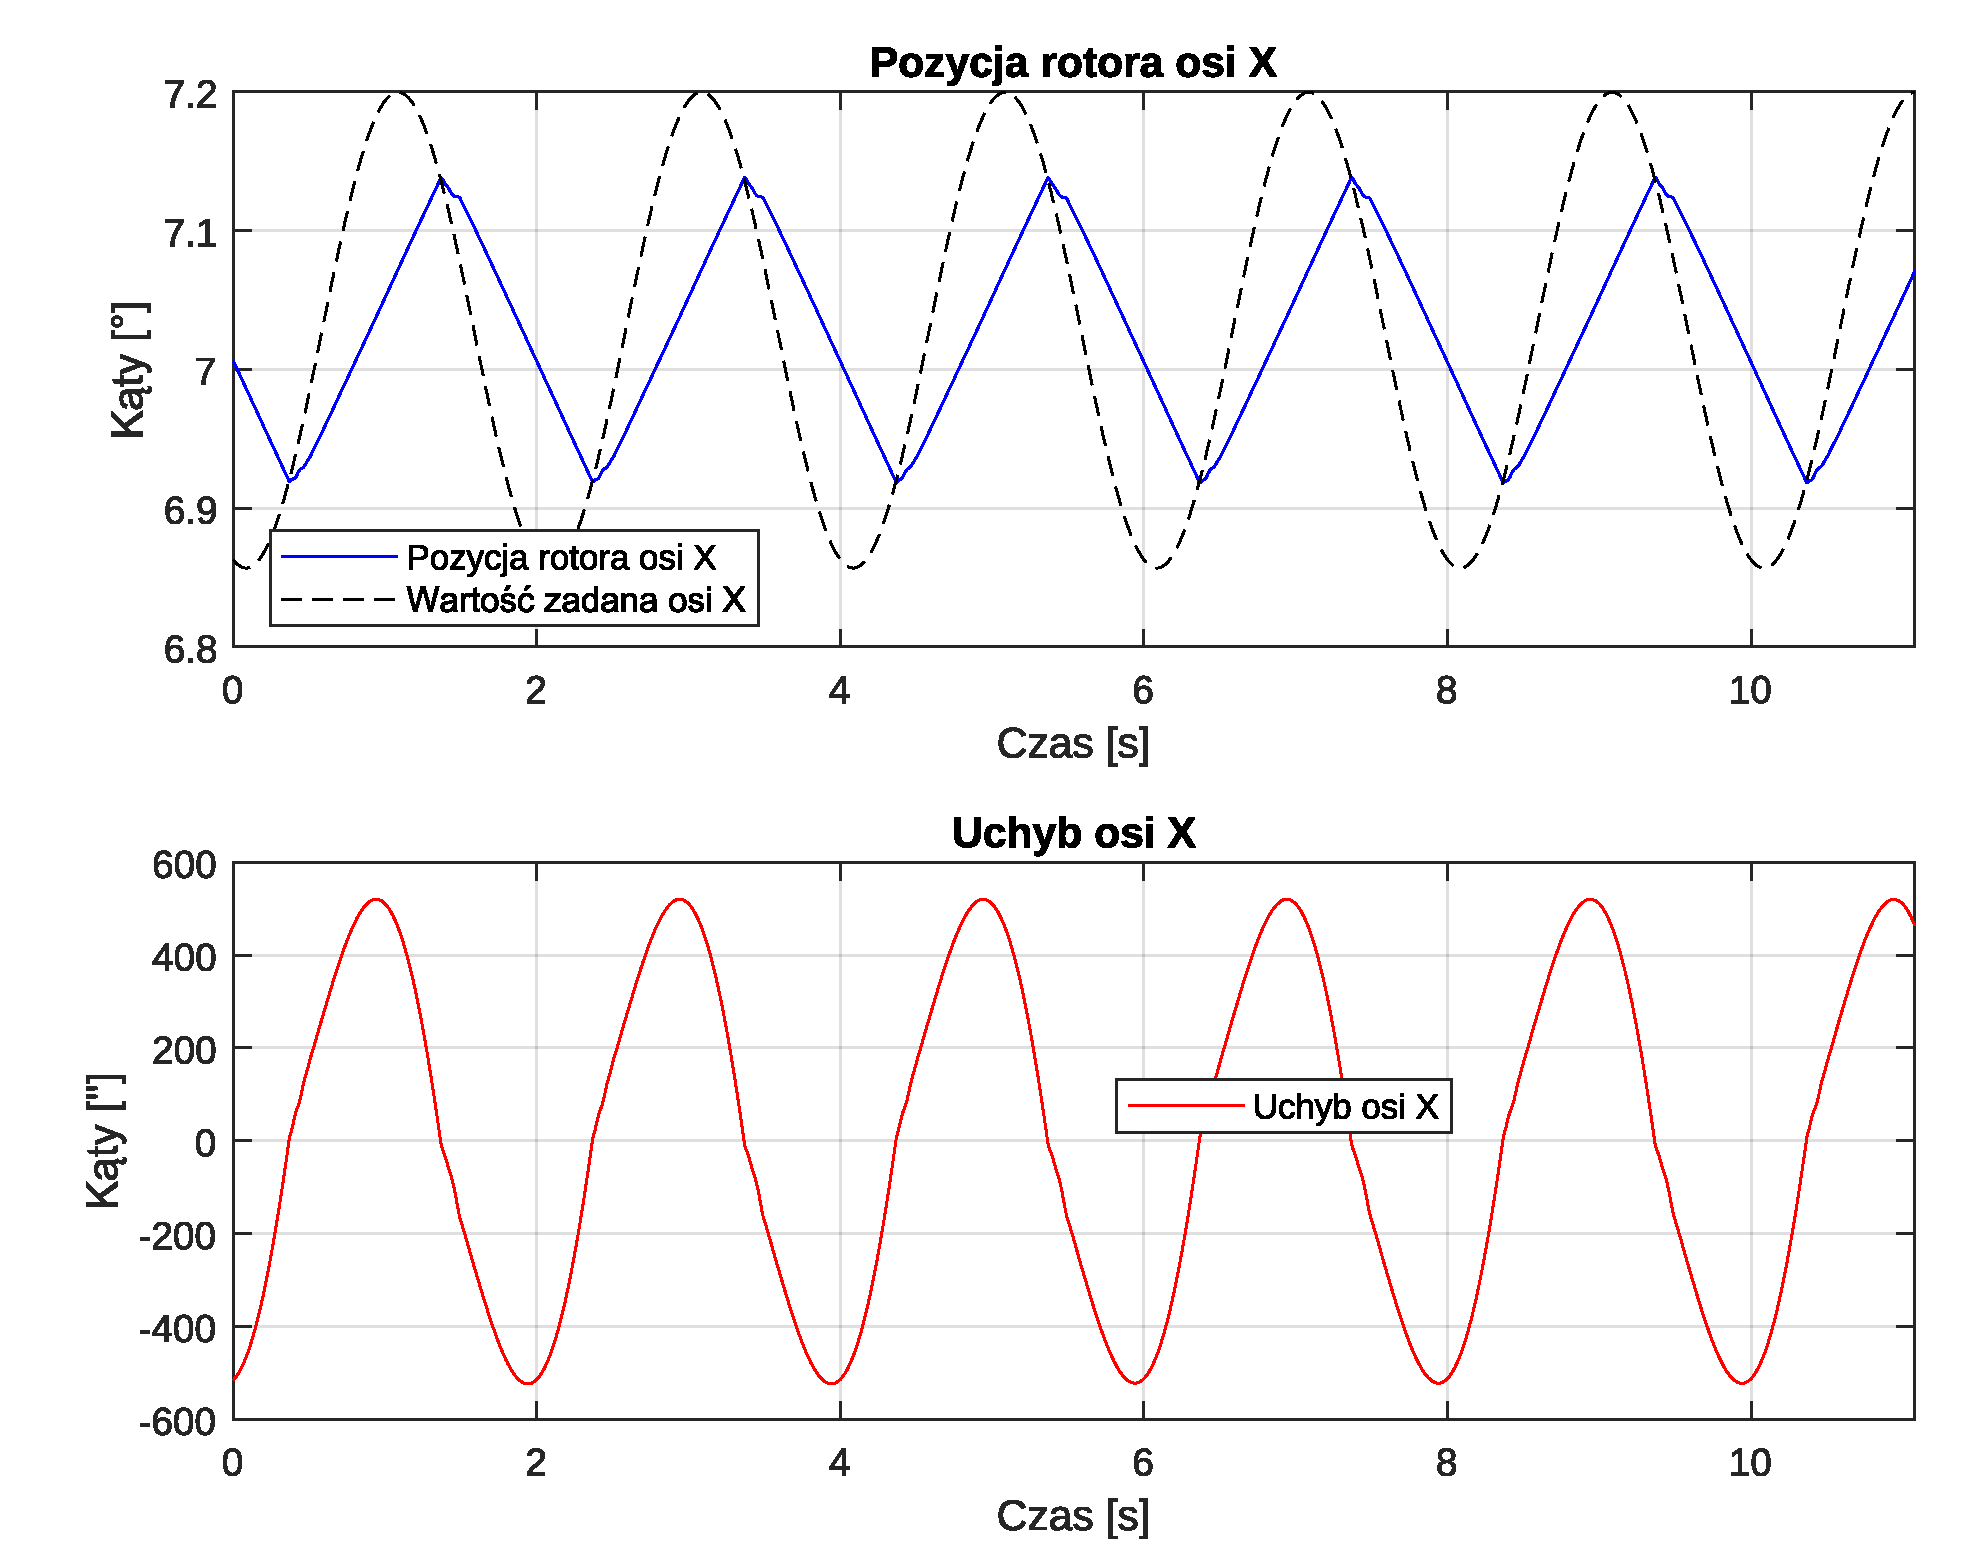
\includegraphics{testy/wykresy_inżynierka/sinus2sX.pdf}}
    \label{fig:schemat blokowy pobierania danych2}
    \caption{Przebiegi dla trajektorii sinusoidalnej o okresie 2 sekund na osi X.}
\end{figure}

\begin{figure}[H]
    \centering
    \resizebox{12cm}{!}{
    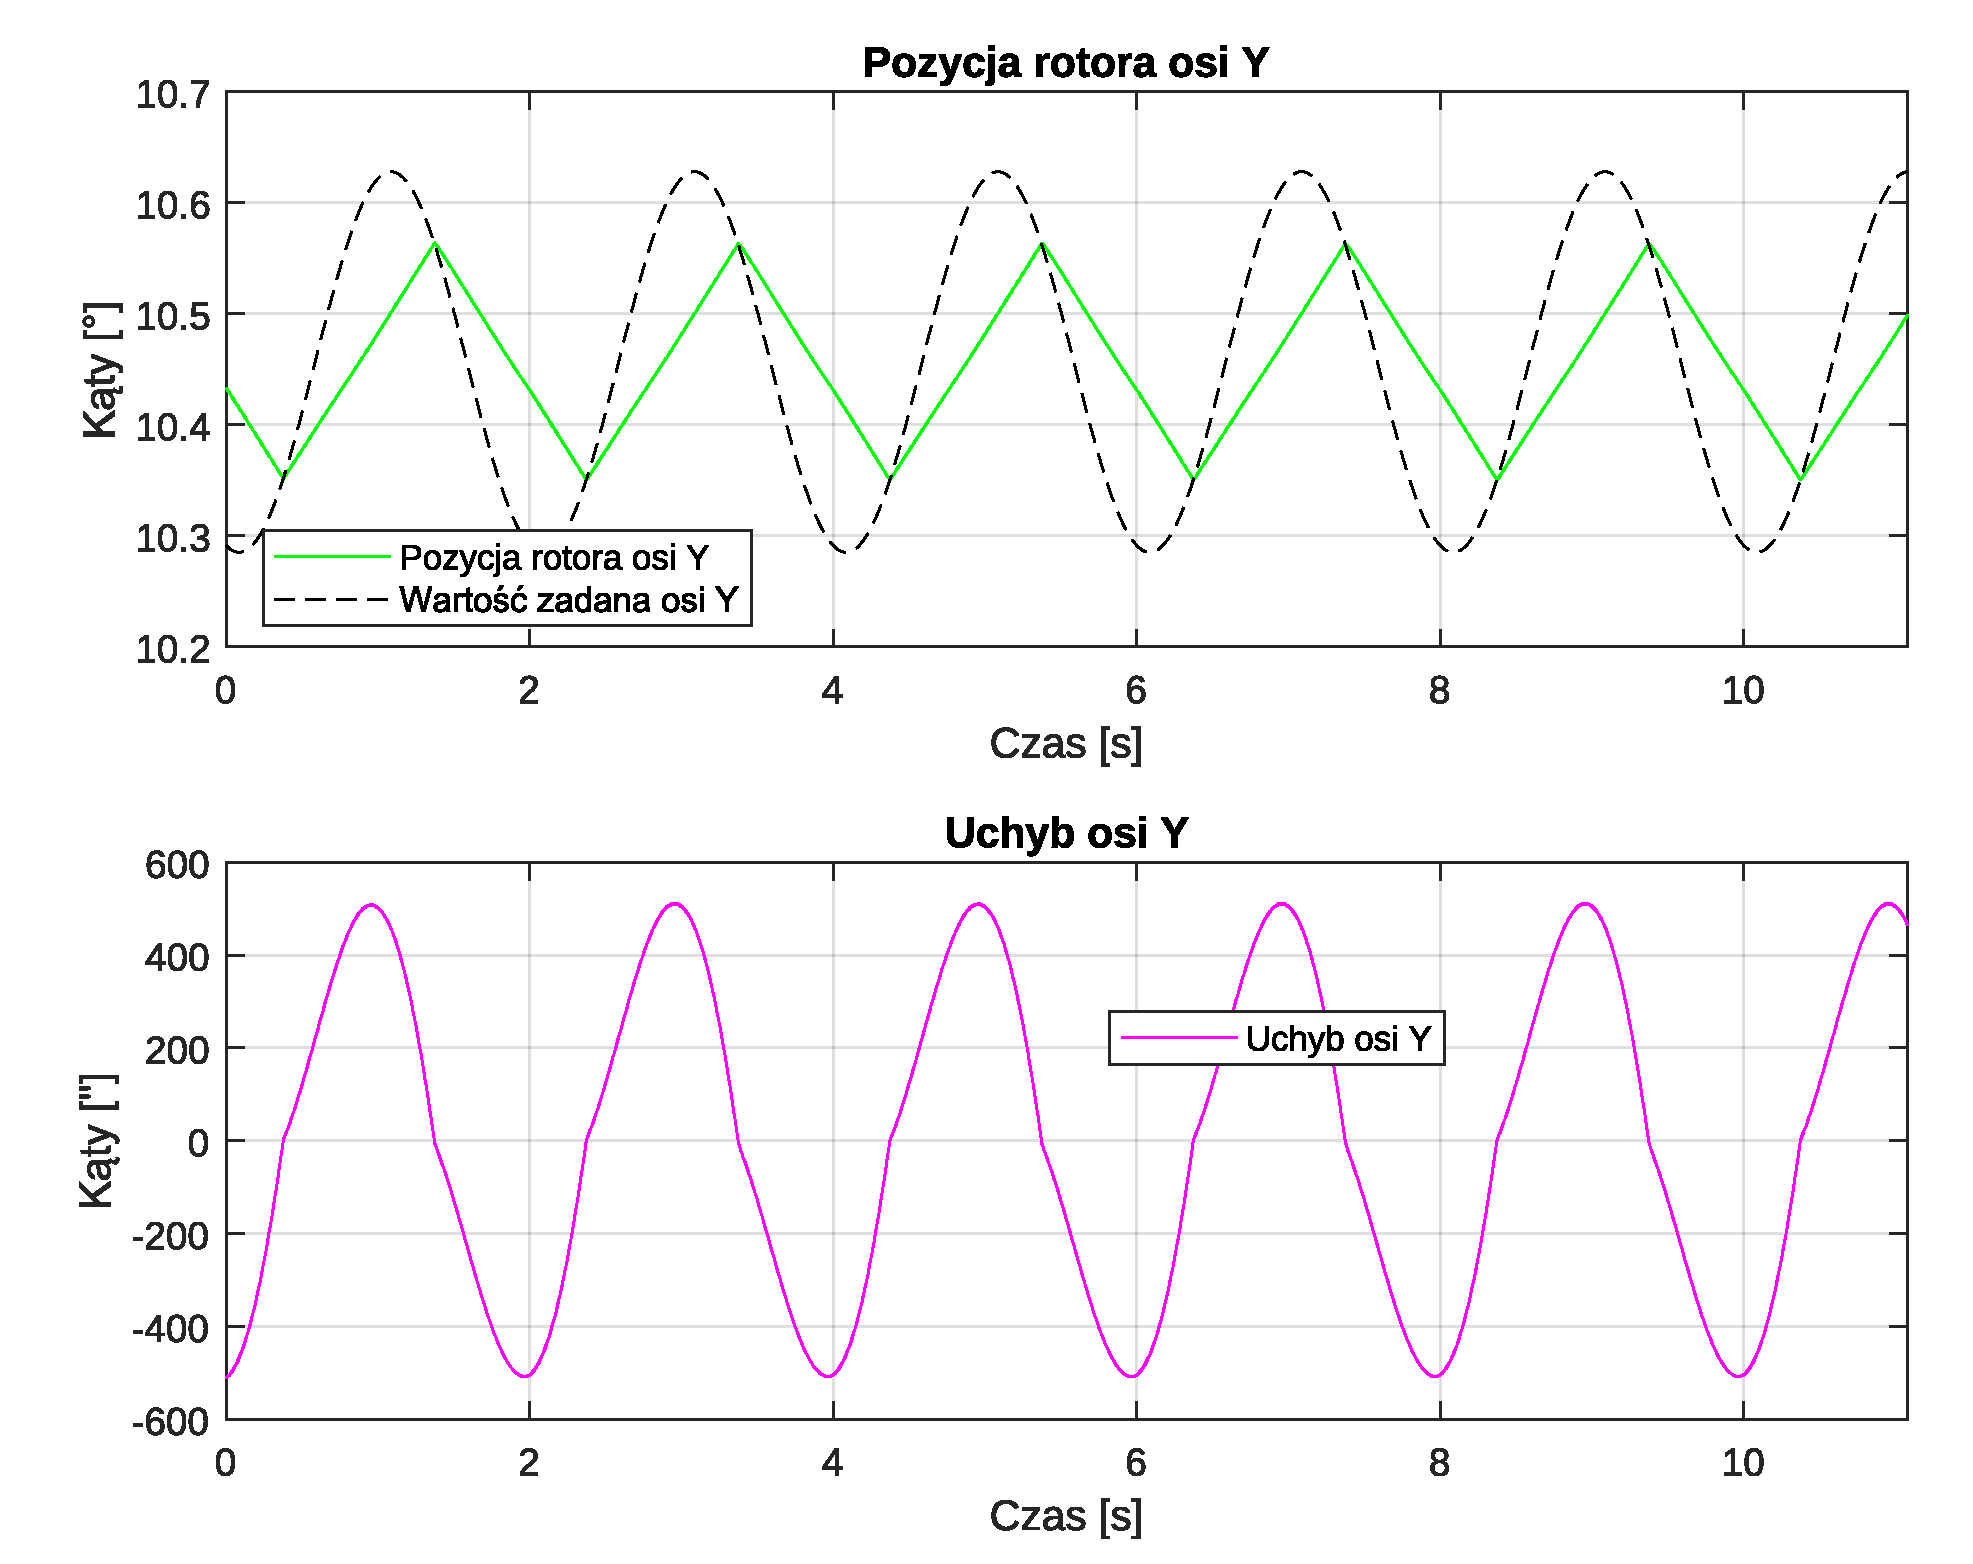
\includegraphics{testy/wykresy_inżynierka/sinus2sY.pdf}}
    \label{fig:schemat blokowy pobierania danych2}
    \caption{Przebiegi dla trajektorii sinusoidalnej o okresie 2 sekund na osi Y.}
\end{figure}

\begin{figure}[H]
    \centering
    \resizebox{12cm}{!}{
    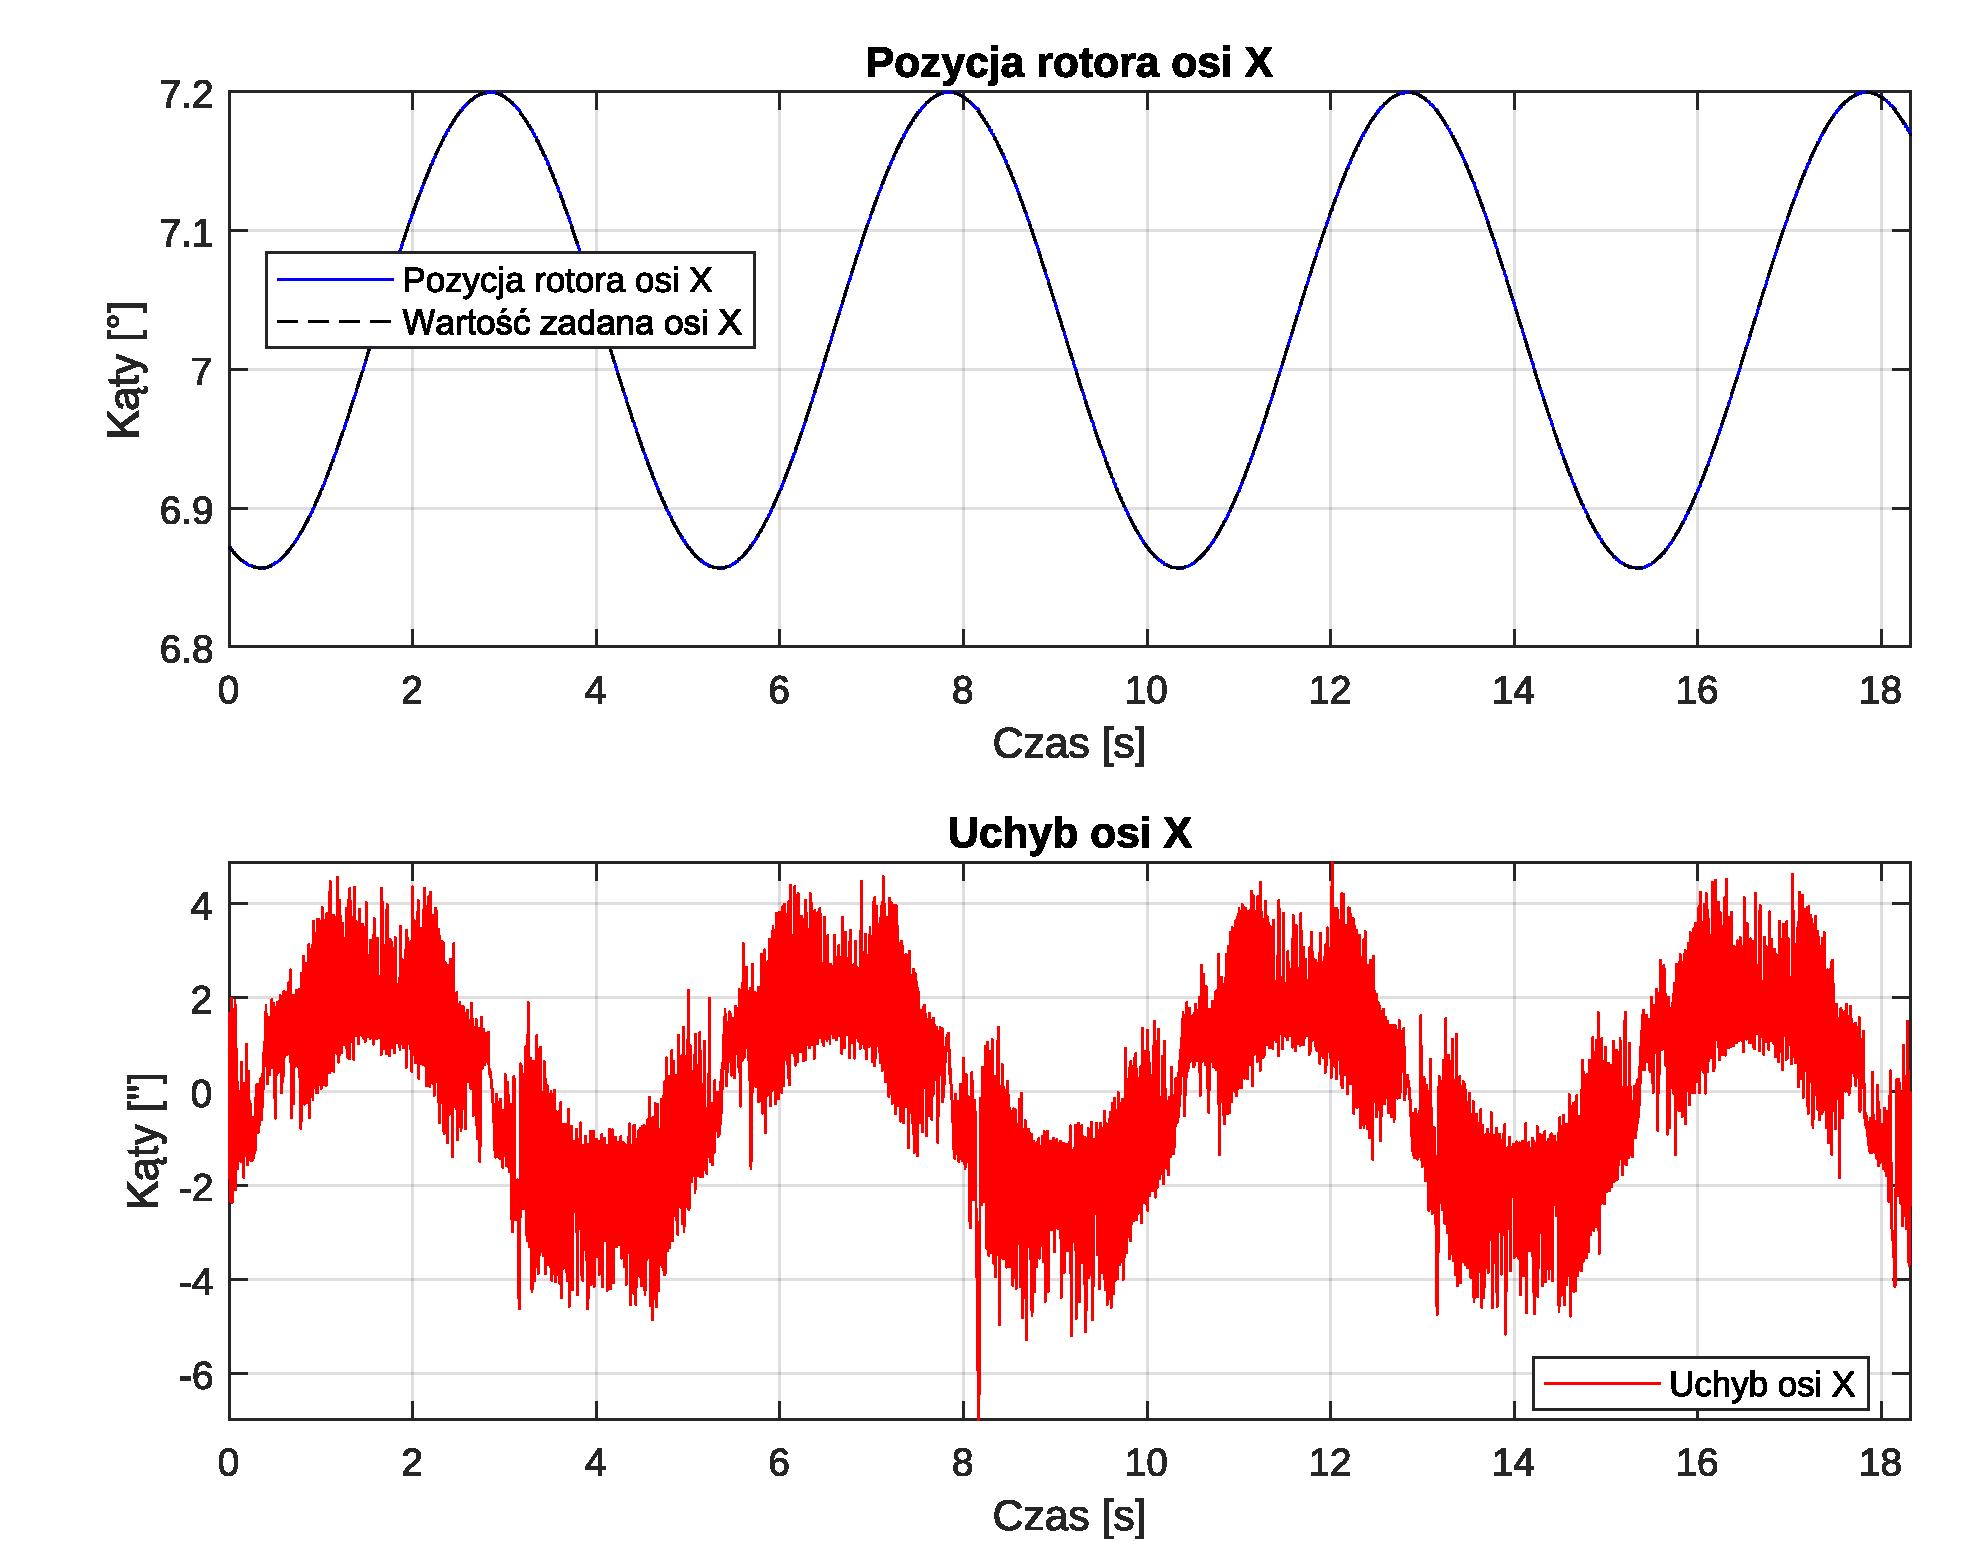
\includegraphics{testy/wykresy_inżynierka/sinus5sX.pdf}}
    \caption{Przebiegi dla trajektorii sinusoidalnej o okresie 5 sekund na osi X.}
    \label{fig:schemat blokowy pobierania danych2}
\end{figure}

\begin{figure}[H]
    \centering
    \resizebox{12cm}{!}{
    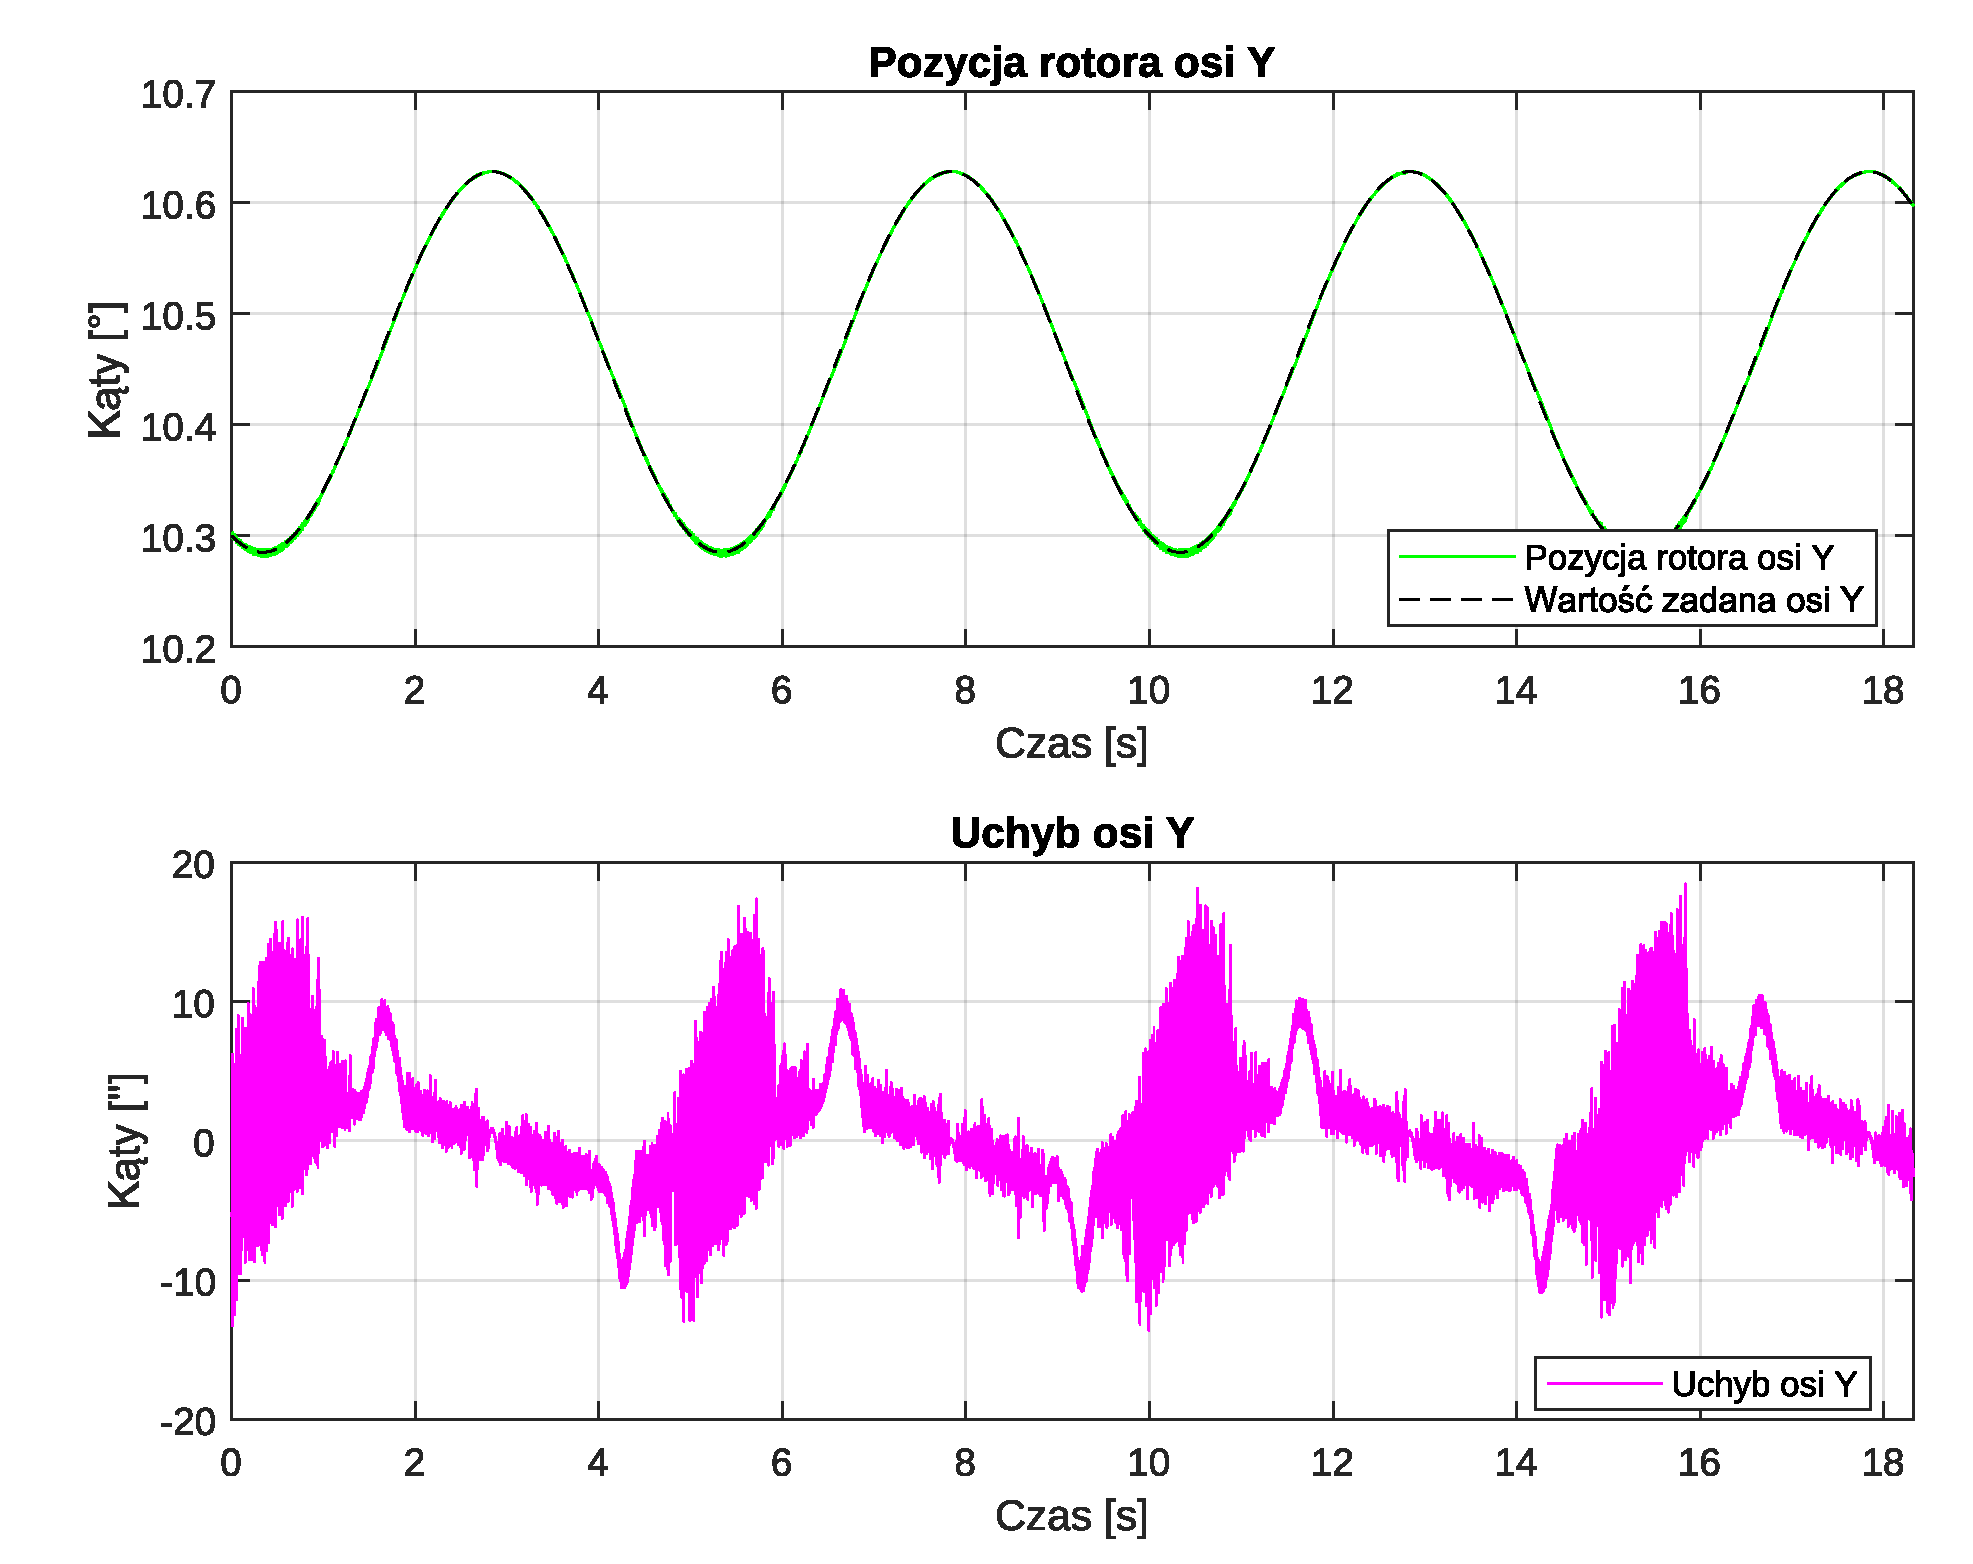
\includegraphics{testy/wykresy_inżynierka/sinus5sY.pdf}}
    \caption{Przebiegi dla trajektorii sinusoidalnej o okresie 5 sekund na osi Y.}
    \label{fig:schemat blokowy pobierania danych2}
\end{figure}

\begin{figure}[H]
    \centering
    \resizebox{12cm}{!}{
    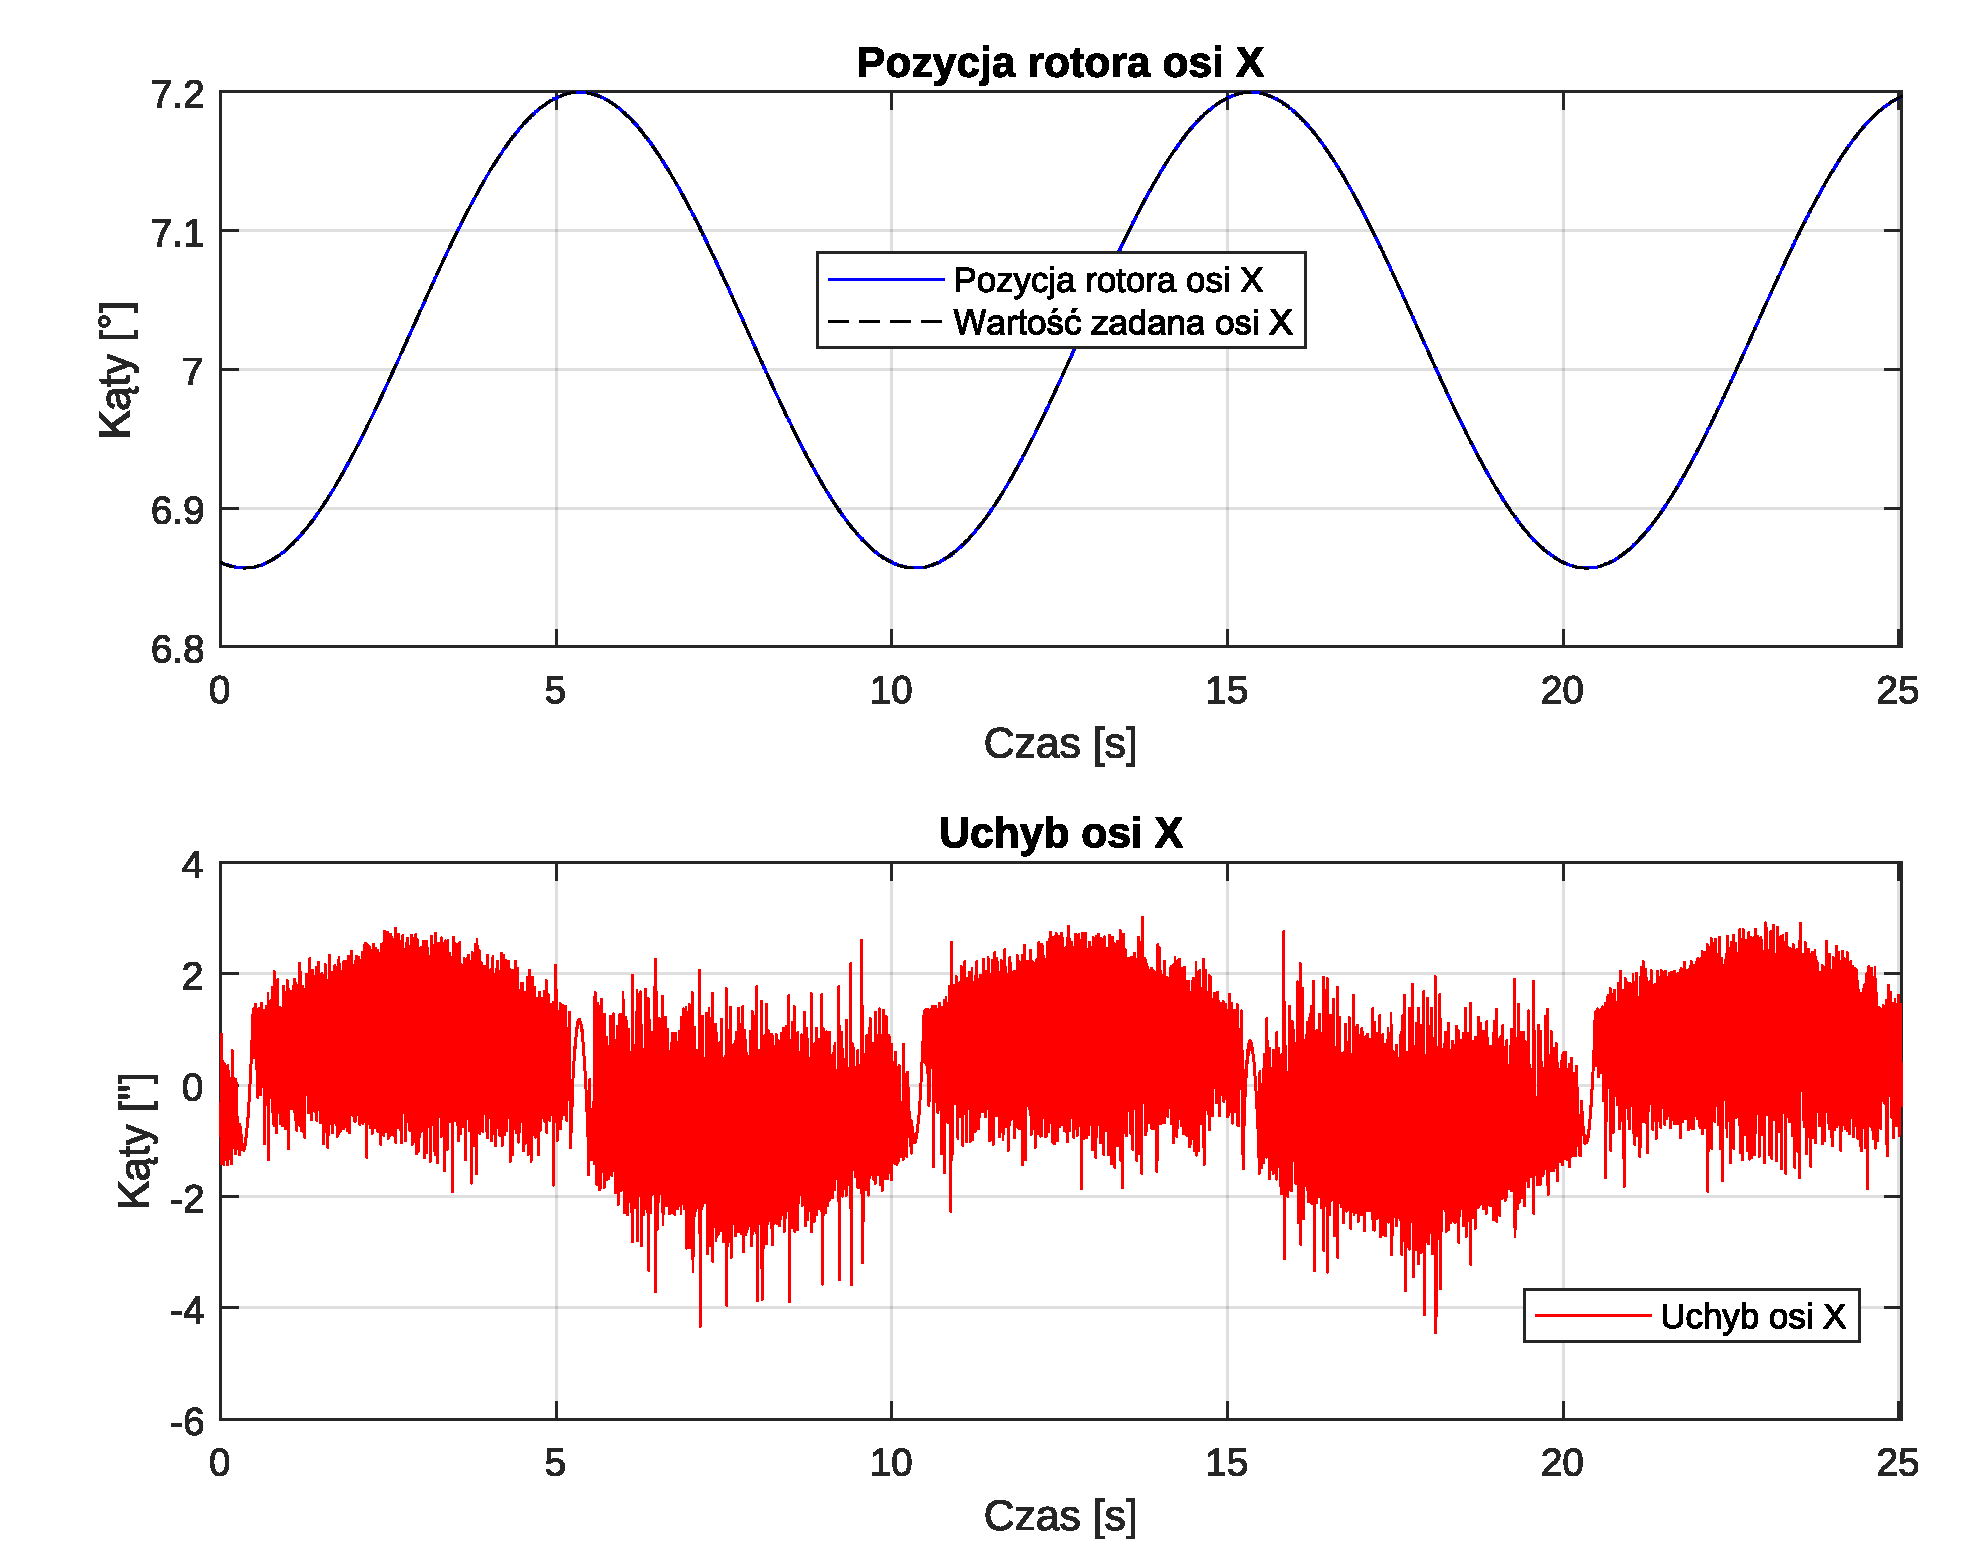
\includegraphics{testy/wykresy_inżynierka/sinus10sX.pdf}}
    \label{fig:schemat blokowy pobierania danych2}
    \caption{Przebiegi dla trajektorii sinusoidalnej o okresie 10 sekund na osi X.}
\end{figure}

\begin{figure}[H]
    \centering
    \resizebox{12cm}{!}{
    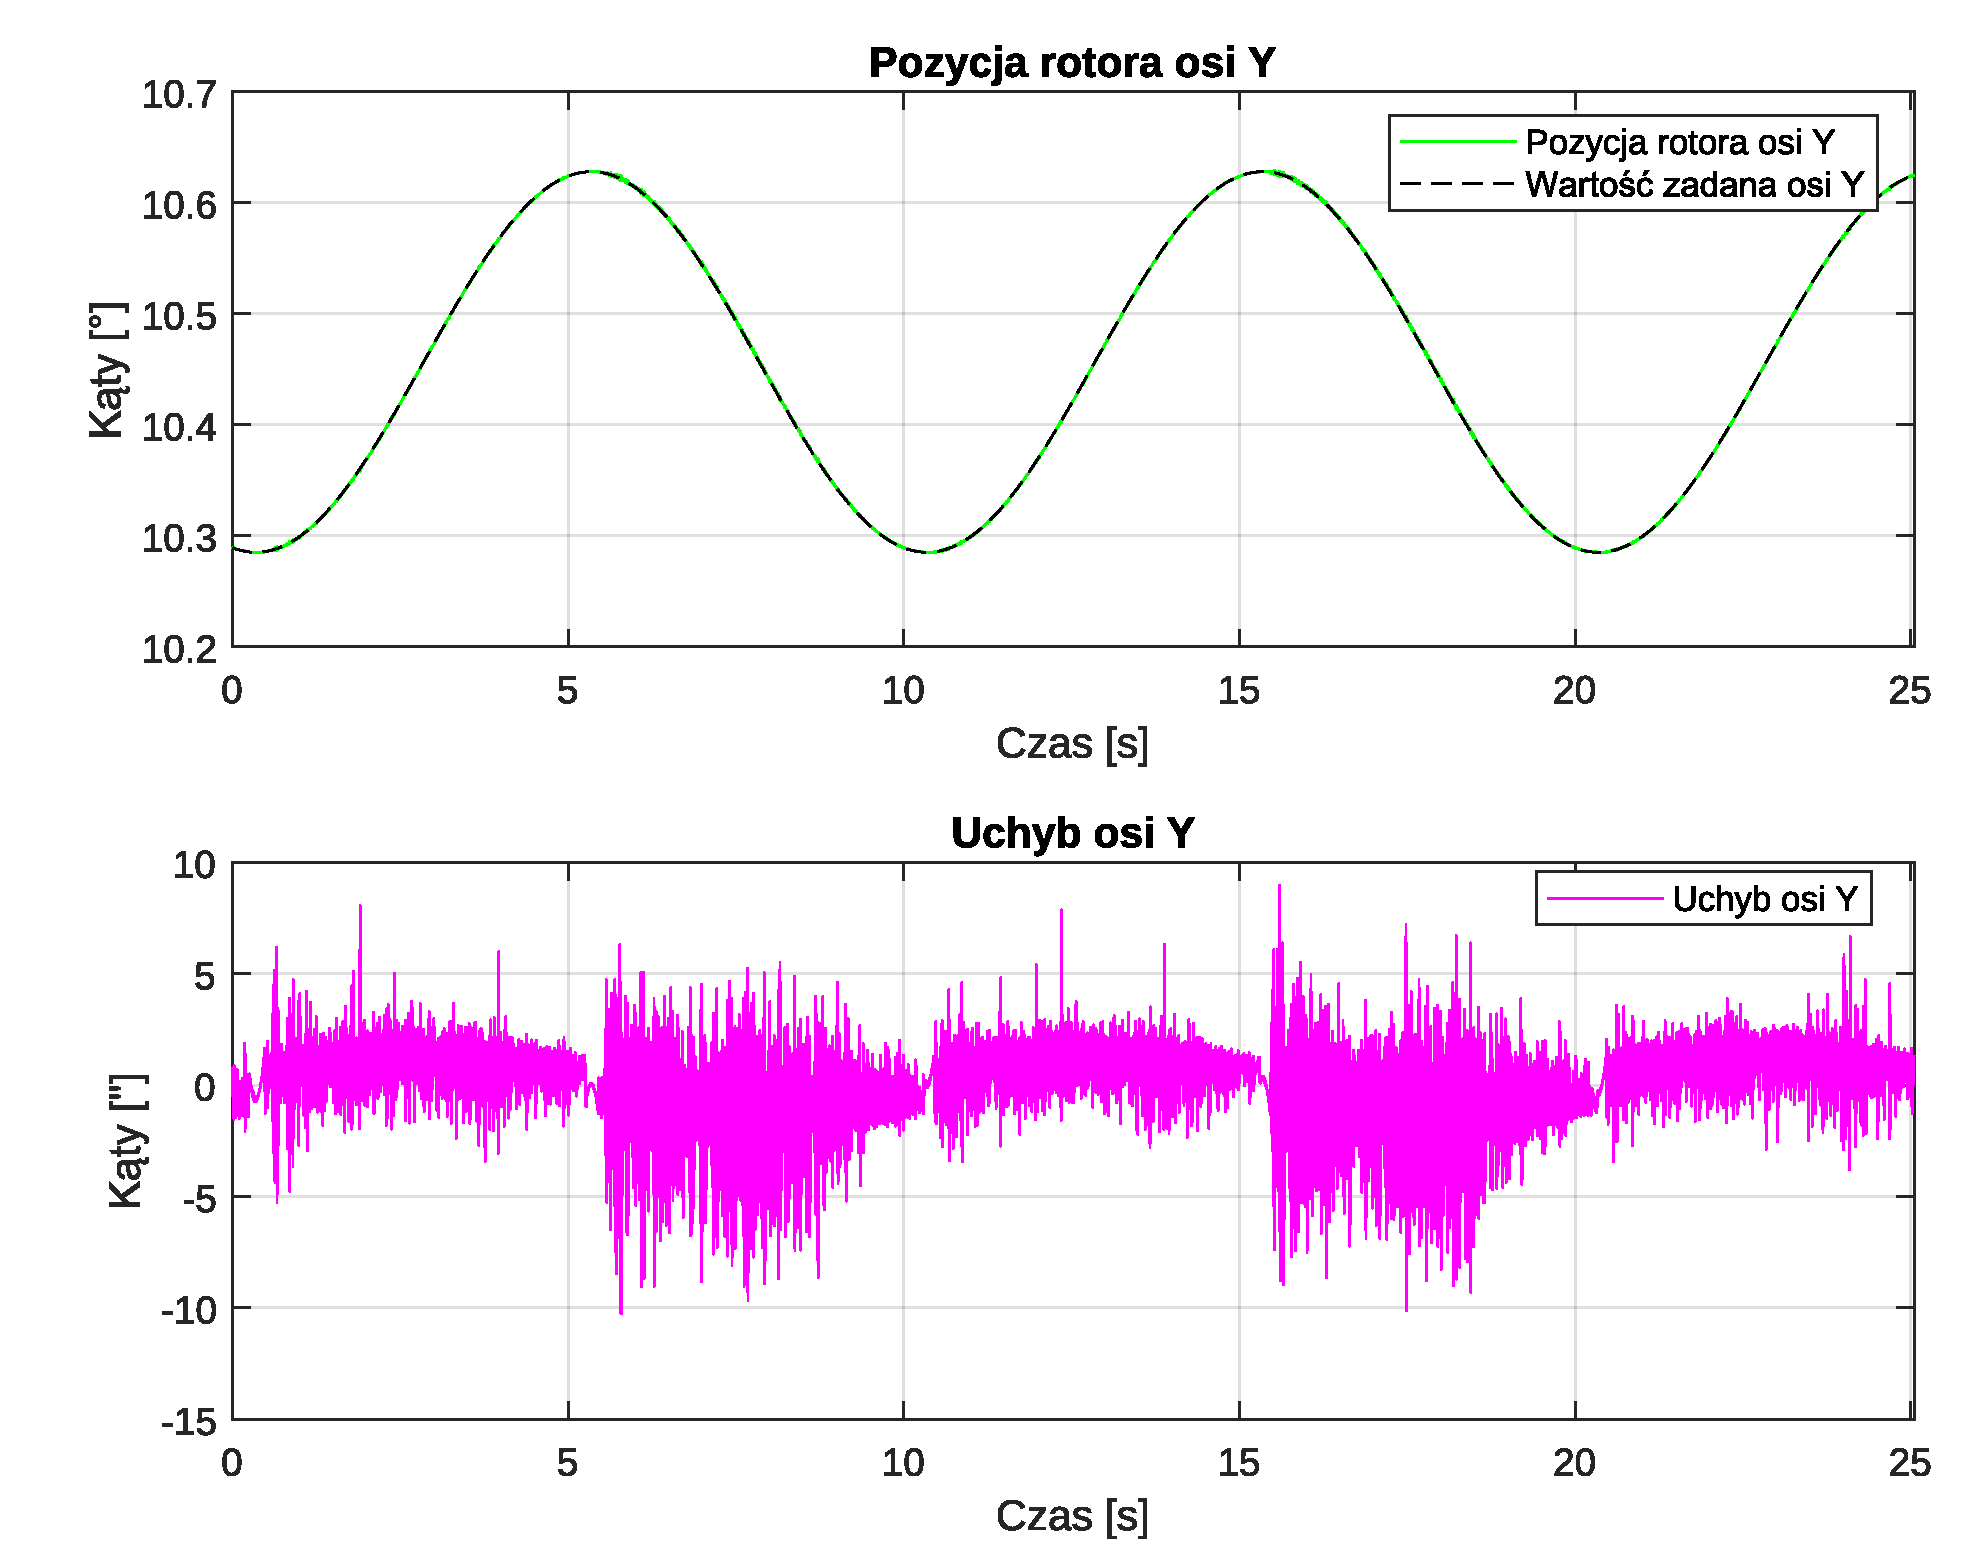
\includegraphics{testy/wykresy_inżynierka/sinus10sY.pdf}}
    \label{fig:schemat blokowy pobierania danych2}
    \caption{Przebiegi dla trajektorii sinusoidalnej o okresie 10 sekund na osi Y.}
\end{figure}

\begin{figure}[H]
    \centering
    \resizebox{12cm}{!}{
    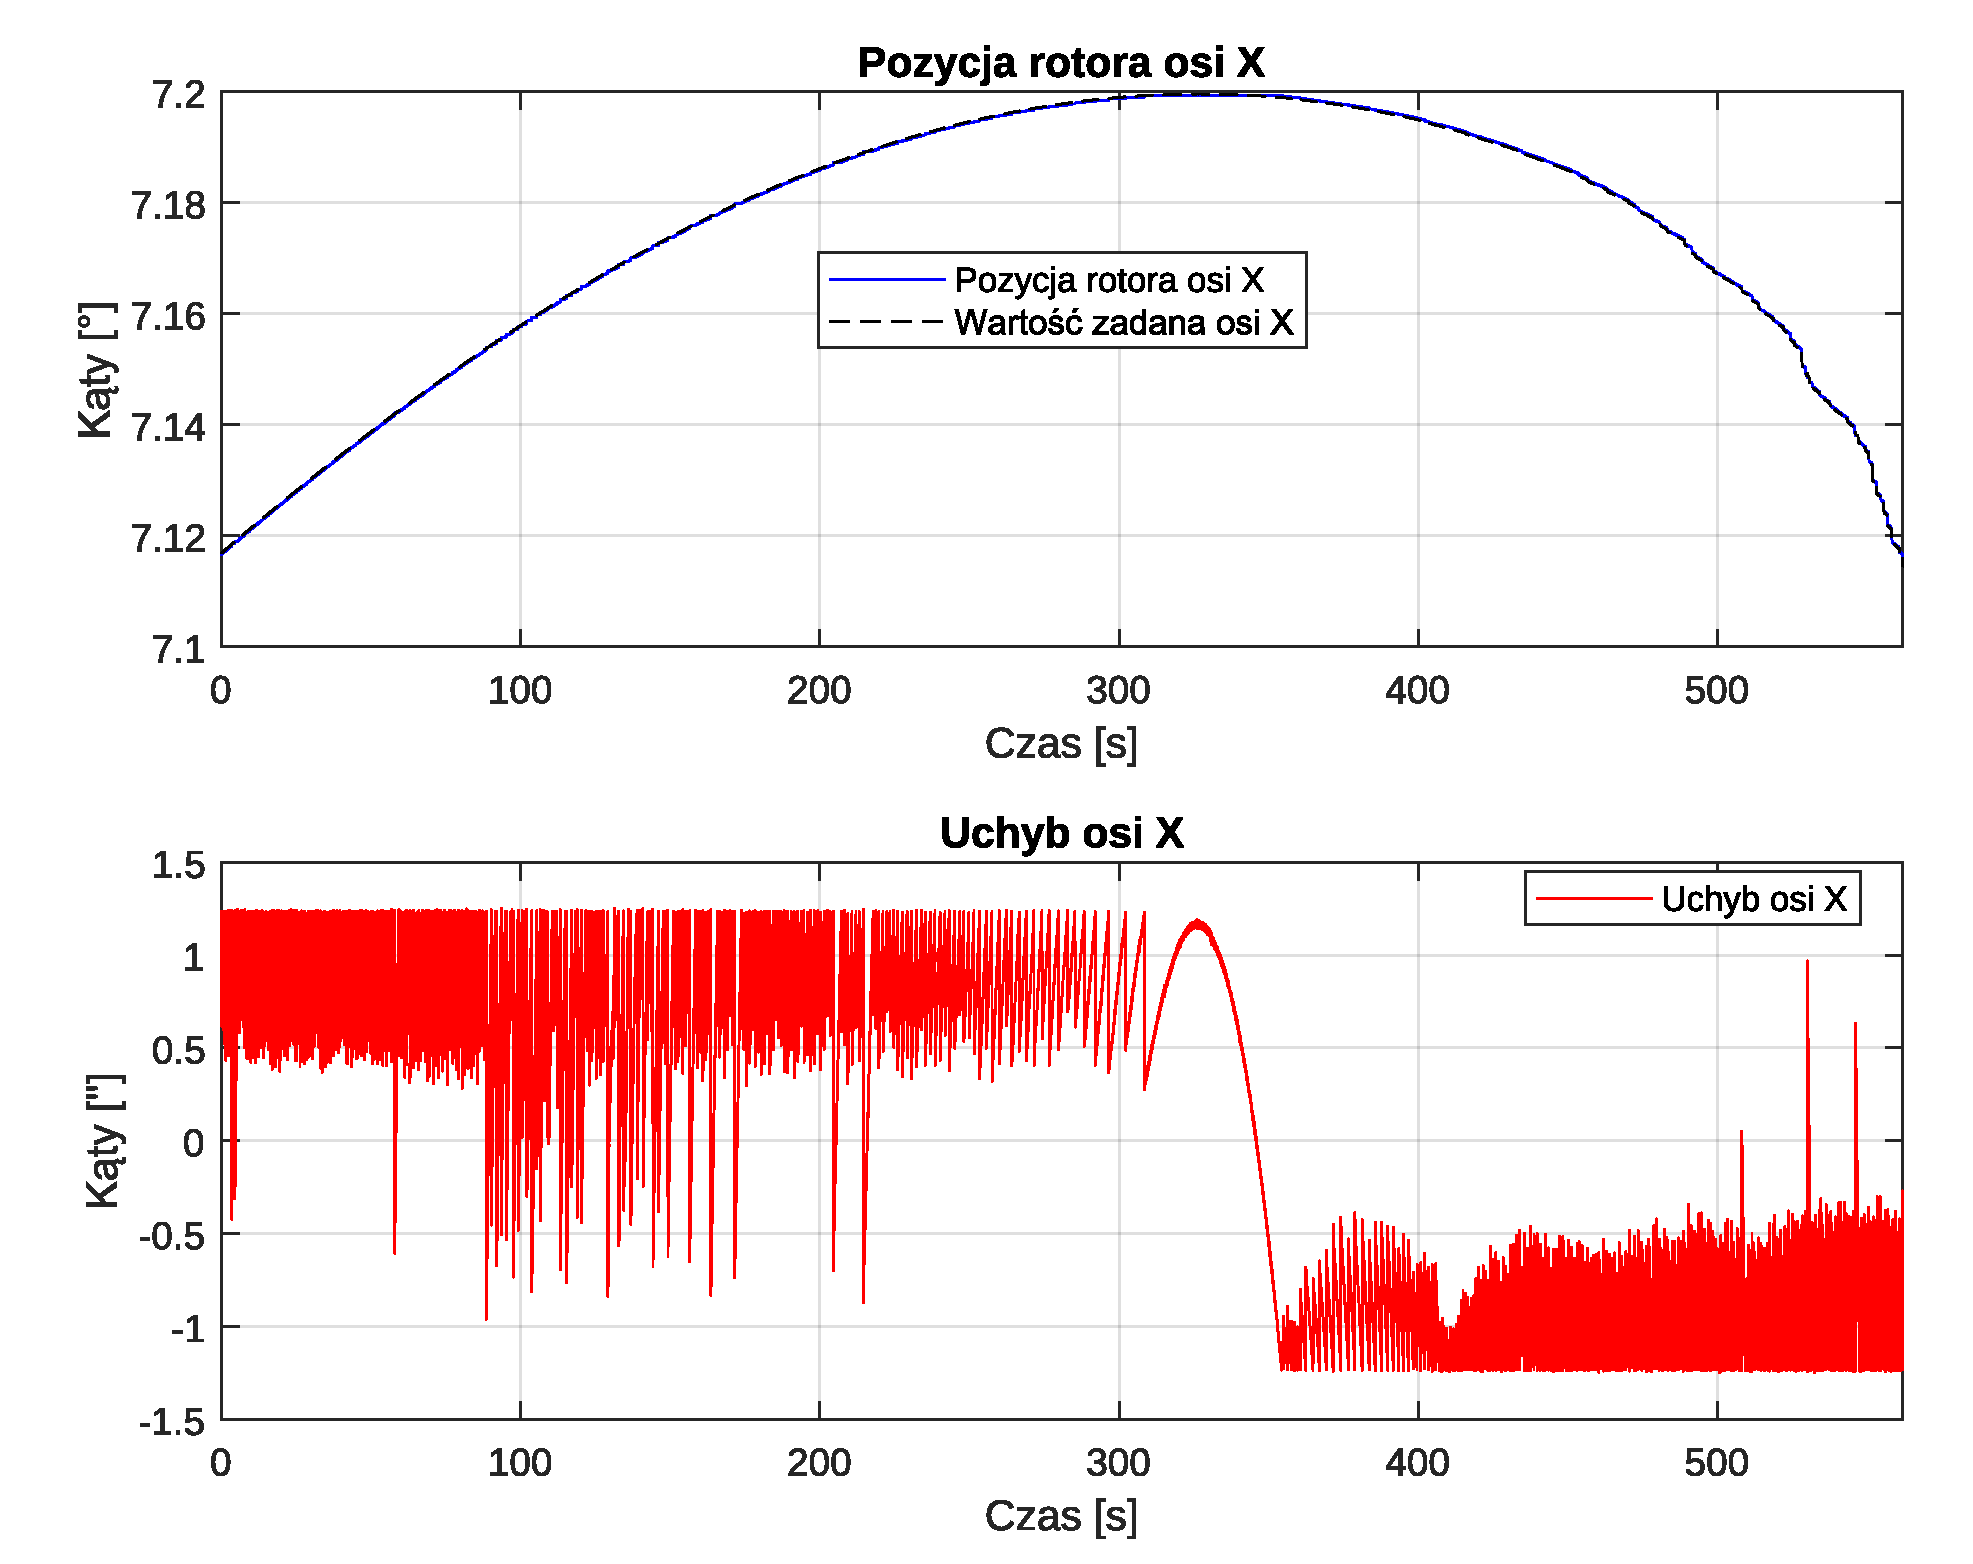
\includegraphics{testy/wykresy_inżynierka/sinus200slongX.pdf}}
    \label{fig:schemat blokowy pobierania danych2}
    \caption{Przebiegi dla trajektorii sinusoidalnej o okresie 200 sekund na osi X.}
\end{figure}

\begin{figure}[H]
    \centering
    \resizebox{12cm}{!}{
    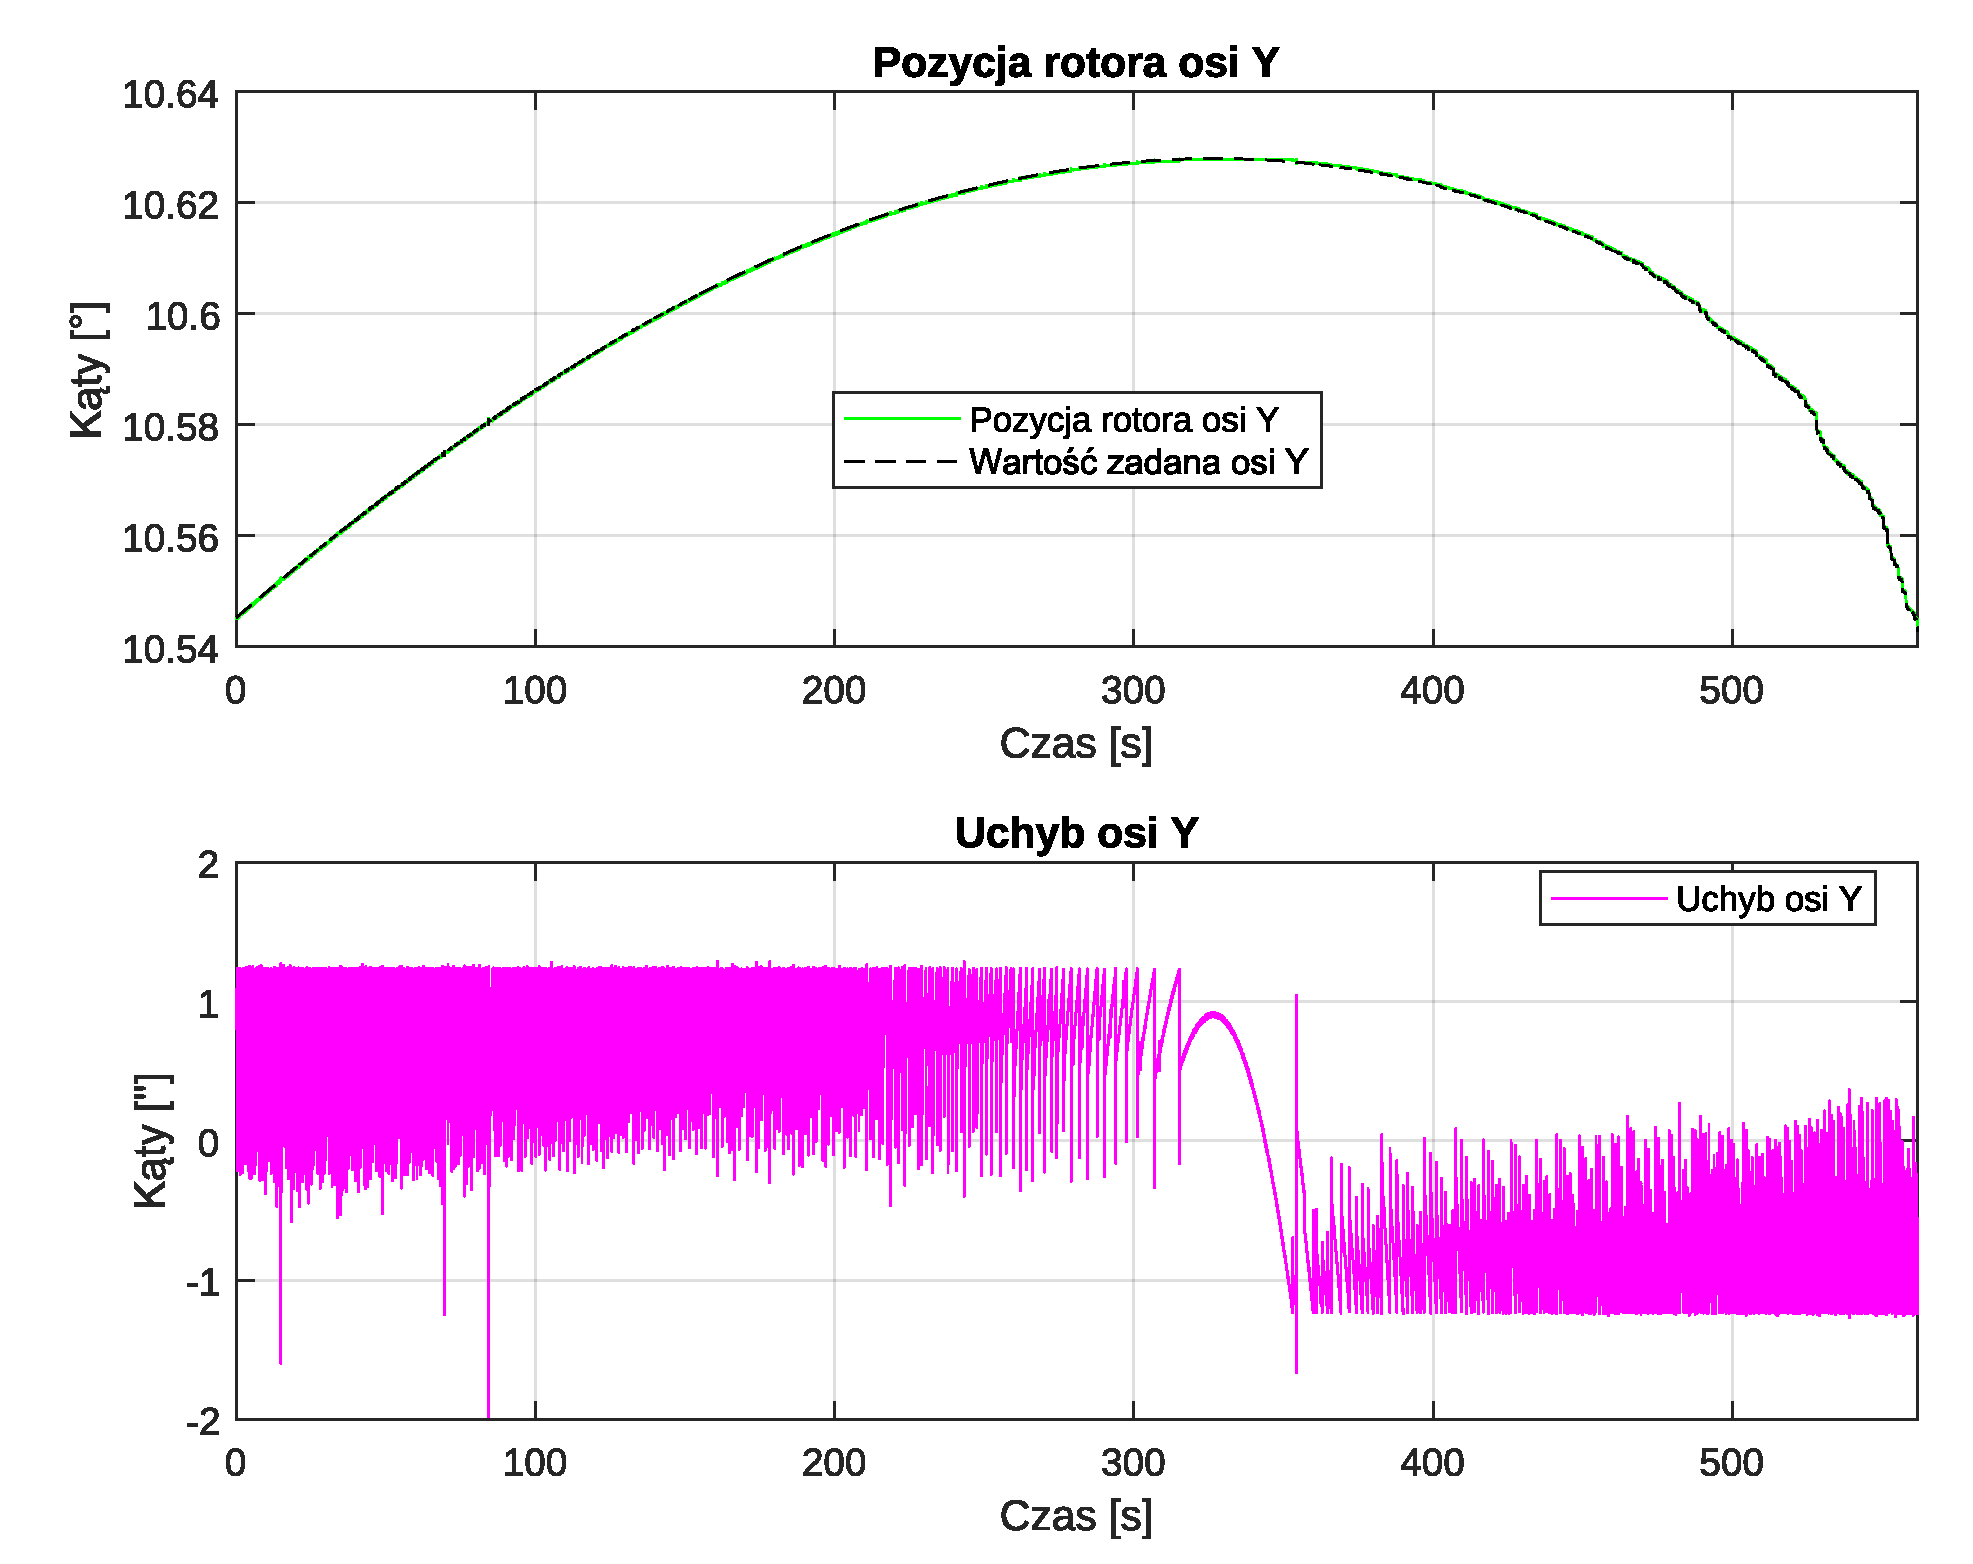
\includegraphics{testy/wykresy_inżynierka/sinus200slongY.pdf}}
    \caption{Przebiegi dla trajektorii sinusoidalnej o okresie 200 sekund na osi Y.}
    \label{fig:Przebiegi dla trajektorii sinusoidalnej o okresie 200 sekund na osi Y.}
\end{figure}

\noindent Dla wszystkich rozważanych trajektorii sinusoidalnych występuje uchyb, który wynika z obecności strefy nieczułości. Dla mniejszych częstotliwości trajektorii sinusoidalnej błąd zawiera się w zakresie zbliżonym do użytej strefy nieczułości (dla bardzo wolnych trajektorii przebieg uchybu praktycznie pozostaje wewnątrz tej strefy - szczególnie to widać na przebiegu \ref{fig:Przebiegi dla trajektorii sinusoidalnej o okresie 200 sekund na osi Y.}). Wynika to z zastosowanej strategii sterowania i nieciągłości pracy regulatora. Dla wyższych częstotliwości układ regulacji przestaje nadążać za trajektorią, co potwierdzają przebiegi \ref{fig:Przebiegi dla trajektorii sinusoidalnej o okresie 1 sekund na osi X.} i \ref{fig:Przebiegi dla trajektorii sinusoidalnej o okresie 1 sekund na osi Y.}. Uchyb dla przebiegów na osi X i Y jest niesymetryczny z powodu cechy konstrukcyjnej.


% Przy różnych częstotliwościach błąd występuje stale, co wynika z cyklicznego generowania sinusa przez mikroprocesor. Po prostu przy zmniejszeniu częstotliwości błąd utrzymuje się stale przez co te wykresy mają większą plamę jakby (analogicznie przy większych). Przy odpowiednio bardzo małej częstotliwości i przybliżeniu punktu odgięcia trajektorii sinusoidalnej widać jak trajektoria próbuje nadążyć i z rachunku referencyjna minus zadana uchyb zmienia wartość na przeciwną, stworzy się taka histereza wtedy co mówił Pazderski jakby ją przyspieszyć wiesz ocb. Po uchybie to widać, zacznie się zmieniać w histerezowo tak jakby w takm kwadracie, w momencie przełączeń zmieni wartość ta histereza. Przy odpowiednio dużych częstotliwościach z kolei układ przestaje nadążać za trajektorią co widać dla wykresu sinus1s. Uchyb już jest dosyć pokaźny. Ja bym powiedział że to ze względu na to jak często odbieramy dane przez spi i , zmiana tych parametrów może nam wpłynąć na precyzję śledzenia, ale obciążymy płytkę w ten sposób bardziej (pole do jakiś tam tych ulepszeń, można to sprawdzić, można to dać do rzeczy jako rozwinięcie pracy, czyli sprawdzenie punktów granicznych). Na moje to nie jest gubienie kroków, bo gubienie kroków to te wartości by musiały przeskakiwać na wykresie a tutaj nic nie skacze (jest na tym samym poziomie jak się coś rzeczywiście zmienia). A no i jeszcze warto wspomnieć o tym, że odkształcający się wykres uchybu w osi y wynika z wady konstrukcyjnej. Ten błąd nie będzie symetrycznie wyglądał, bo jak się wysuwa oś X to Y się napina strasznie i wykres się odkształca. Tam to sprzężenie było przeciwnie więc jak u nas się w X wysuwa to w Y się wsuwa patrząc na wartości, czyli jest git, ta oś Y się napina bo próbuje się skurczyć a że materiał trwały aluminium to nie ma jak i ten błąd jest taki duży w tym momencie na tych wykresach.


\section{Trajektoria prostokątna}
\begin{figure}[H]
    \centering
    \resizebox{12cm}{!}{
    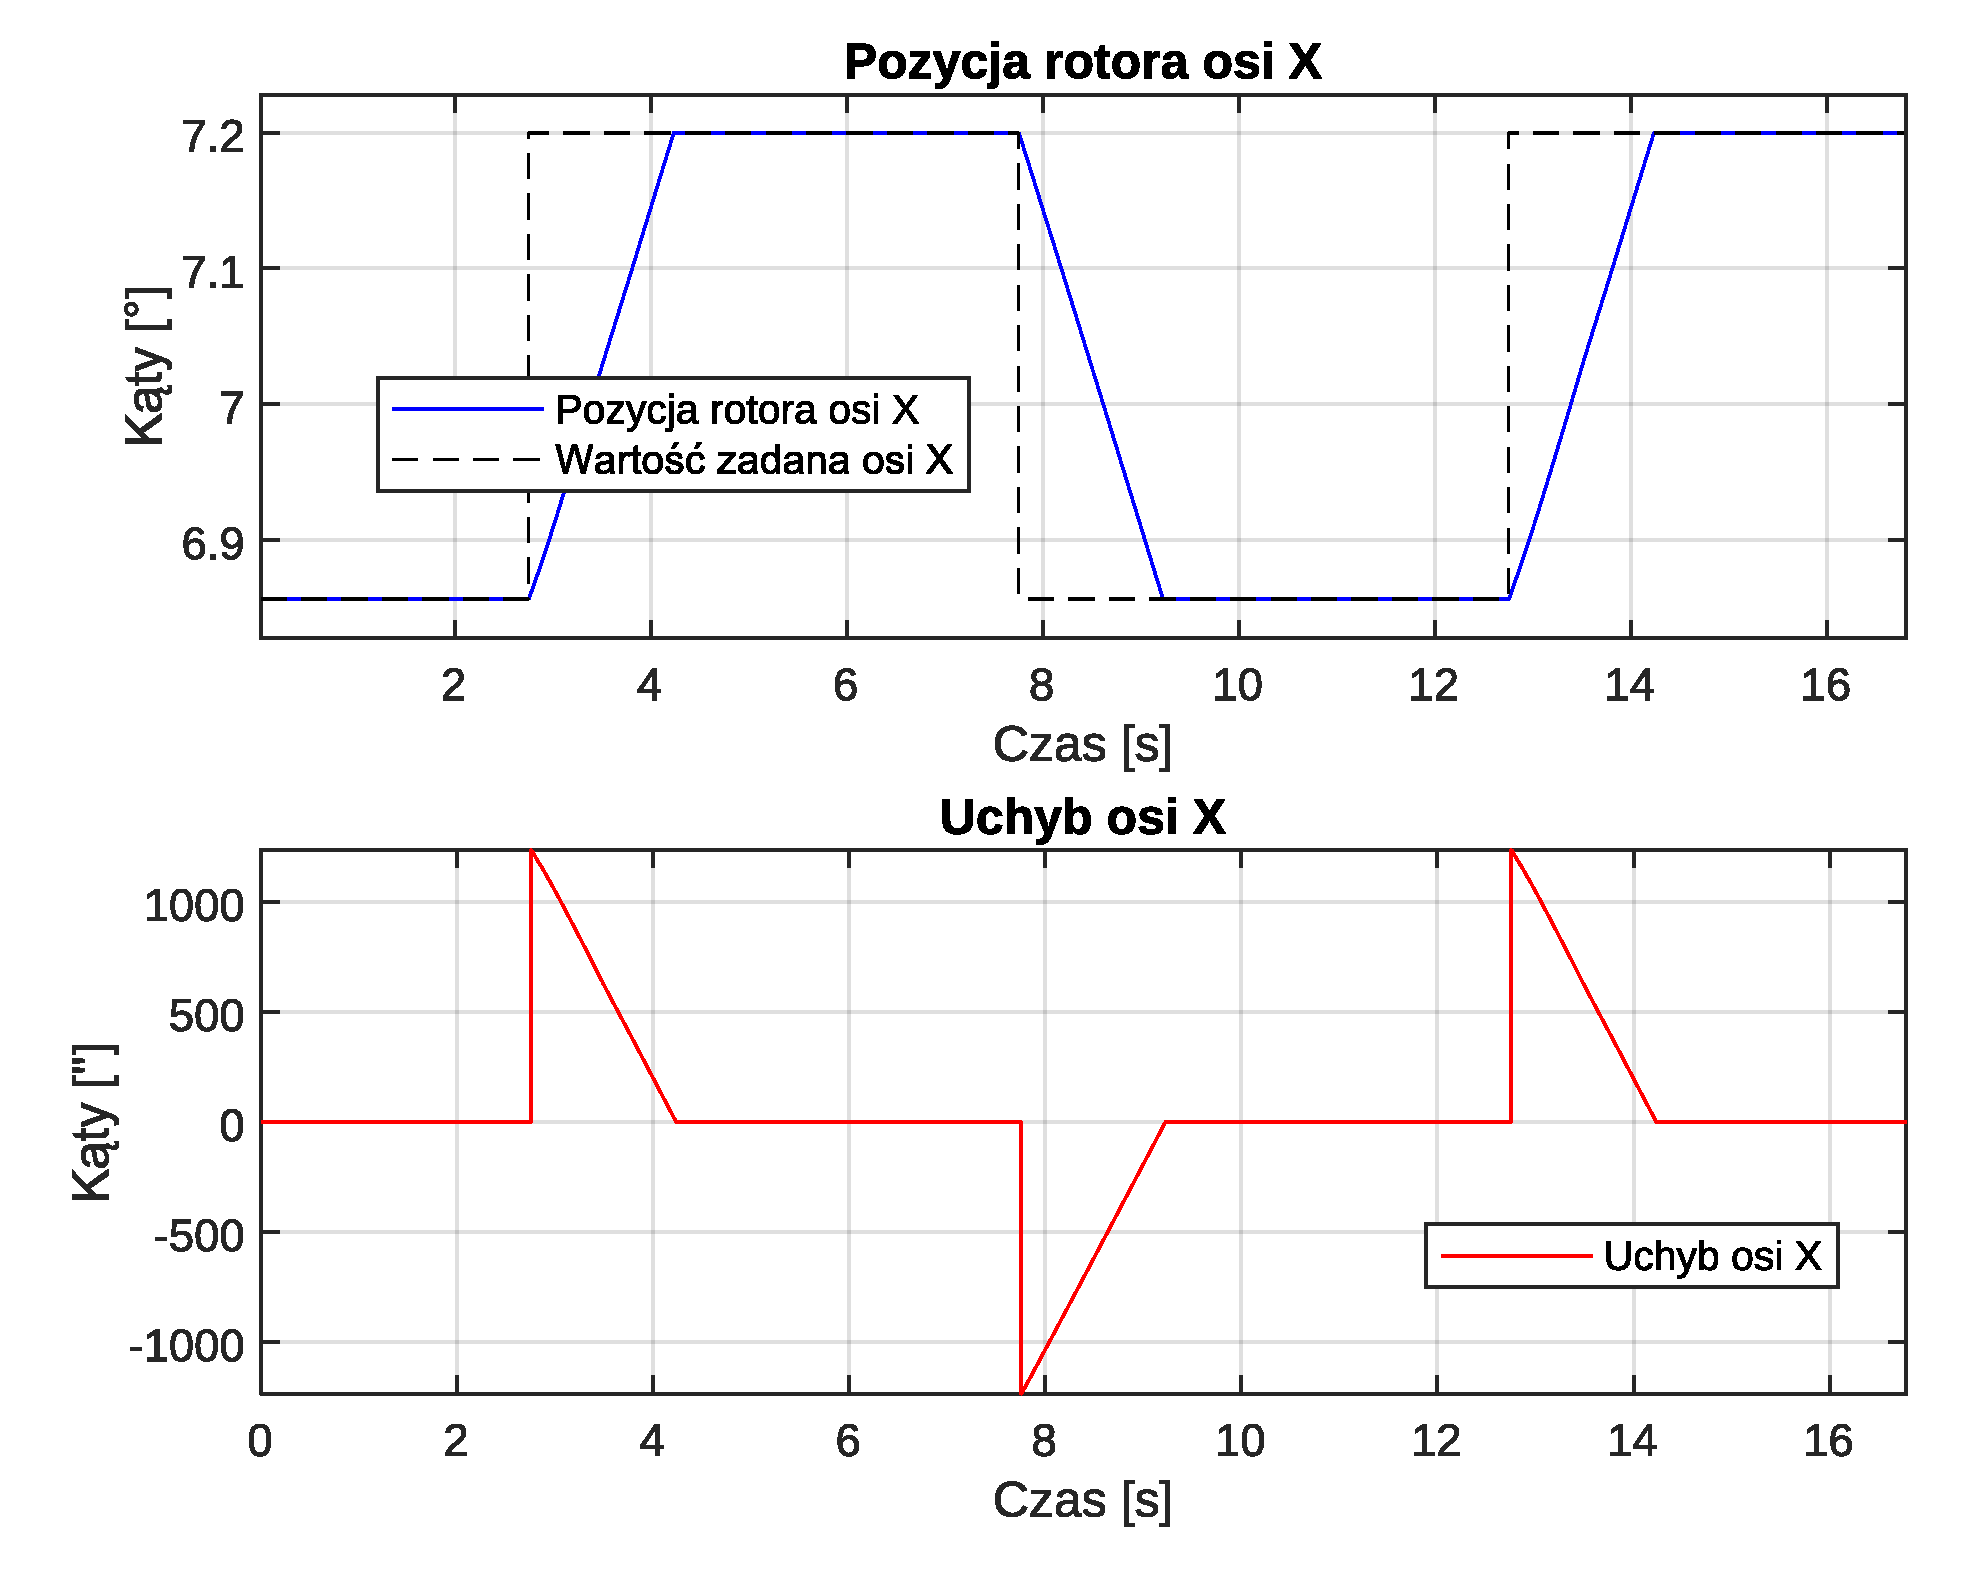
\includegraphics{testy/wykresy_inżynierka/squareX.pdf}}
    \label{fig:schemat blokowy pobierania danych2}
    \caption{Przebiegi dla trajektorii prostokątnej o okresie 10 sekund na osi X.}
\end{figure}

\begin{figure}[H]
    \centering
    \resizebox{12cm}{!}{
    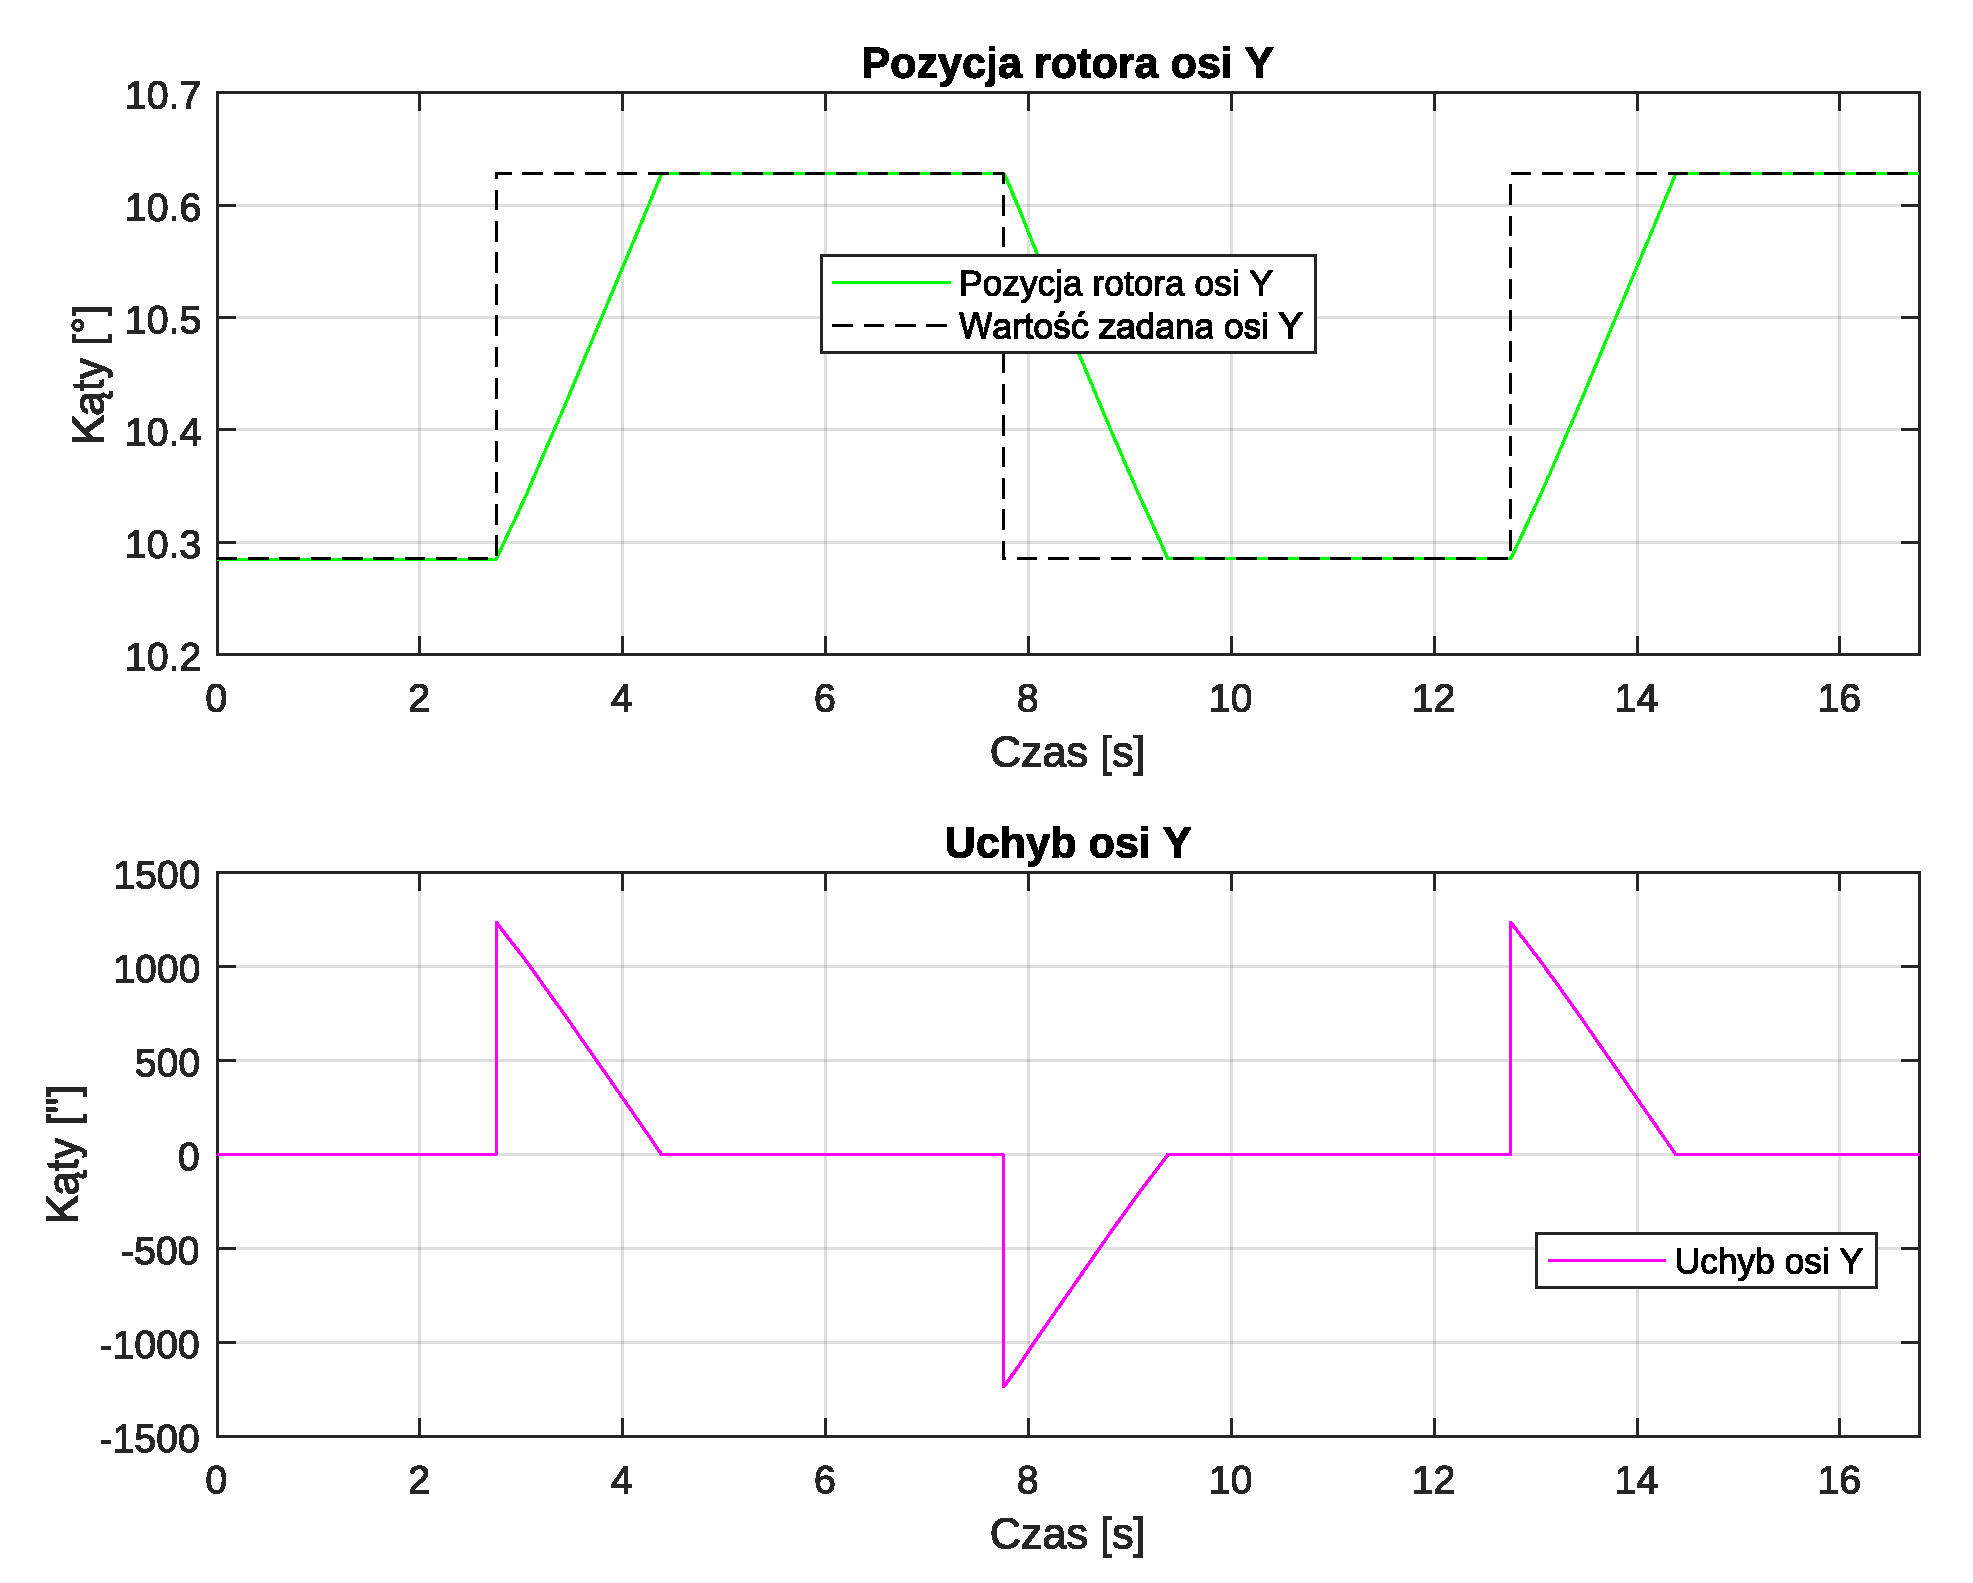
\includegraphics{testy/wykresy_inżynierka/squareY.pdf}}
    \label{fig:schemat blokowy pobierania danych2}
    \caption{Przebiegi dla trajektorii prostokątnej o okresie 10 sekund na osi Y.}
\end{figure}

% W momencie nawrotu, czyli skokowych zmian pozycji, układ dąży do osiągnięcia celu po ponad sekundzie. (nie wiem co tu więcej można powiedzieć). Generalnie jest gicio, działa (tutaj też można wspomnieć, że można się pobawić tymi stałymi czasowymi i przetestować dla jakich częstotliwości zbierania próbek z enkodera i zmienieniu martwej strefy zmieni się stała czasowa i czy to ma wpływ wgl, tutaj imo odległość gra rolę, bo gdyby ten punkt miał być dalej to ten wykres by dalej próbował nadążyć, można da porównania zrobić taki i opisać)  
Zastosowana metoda sterowania silnikiem krokowym powoduje w przybliżeniu stałą prędkość obrotu osi. Podczas dynamicznych zmian wartości zadanej pozycja nie osiąga natychmiast nowej wartości, lecz zmienia się liniowo, to jest silnik musi wykonać odpowiednią liczbę kroków. 

\section{Badanie wpływu większej częstotliwości sterowania pracą silników}

\vspace{1cm}

\begin{center}
    \textbf{Synchronizacja momentu odczytywania danych z sygnałami podawanymi na wejście CLK}
\end{center}

\begin{figure}[H]
    \centering
    \resizebox{16cm}{!}{
    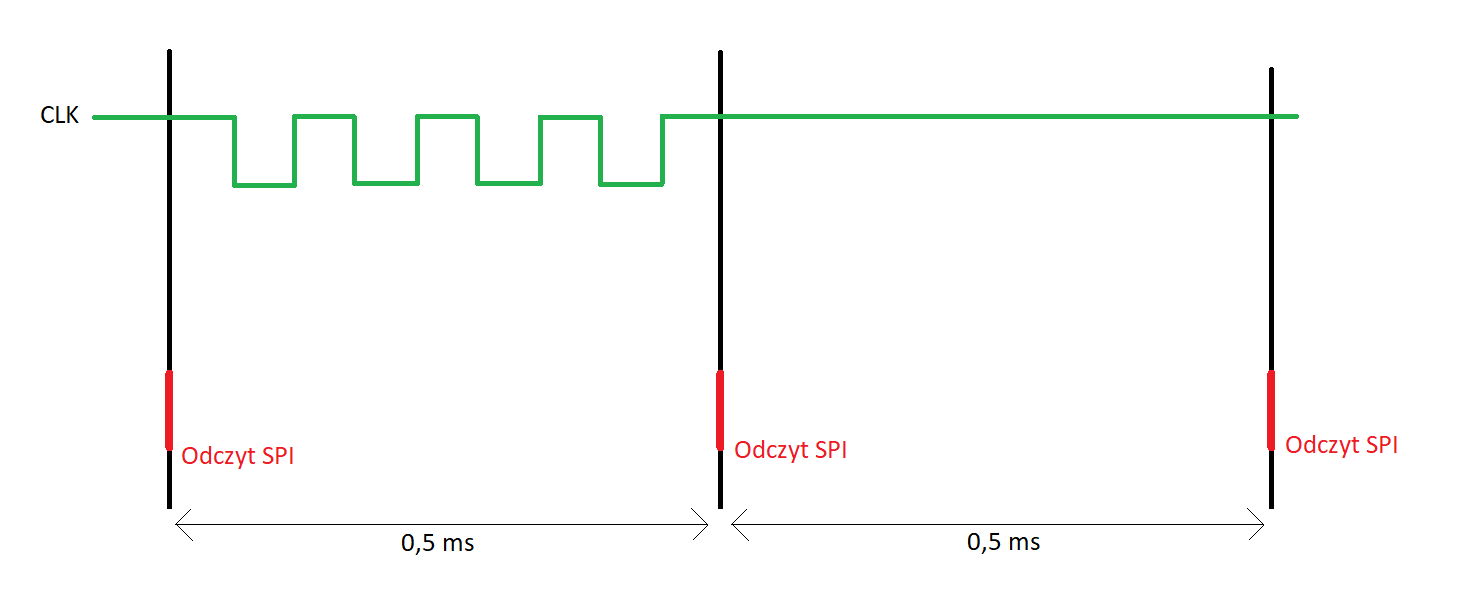
\includegraphics{pictures/image.png}}
    \caption{Sterowanie sygnałem na wejściu CLK.}
    \label{fig:Sterowanie sygnałem na wejściu CLK}
\end{figure}

\noindent W tym eksperymencie pozostawiono częstotliwość próbkowania 2kHz, zmieniano jednak częstotliwość sygnału zegarowego sterującego prędkością przełączania silnika za pomocą niezależnego timera. Powoduje to wprowadzenie pewnego asynchronizmu w sterowaniu, ponieważ tylko niektóry cykl zegara generowany jest na podstawie bieżącej pozycji. Graficzna reprezentacja całego procesu została przedstawiona na rysunku \ref{fig:Sterowanie sygnałem na wejściu CLK}. Tryb synchroniczny nie był implementowany dla częstotliwości próbkowania powyżej 2kHz z uwagi na ograniczone zasoby obliczeniowe mikrokontolera.

\begin{figure}[H]
    \centering
    \resizebox{12cm}{!}{
    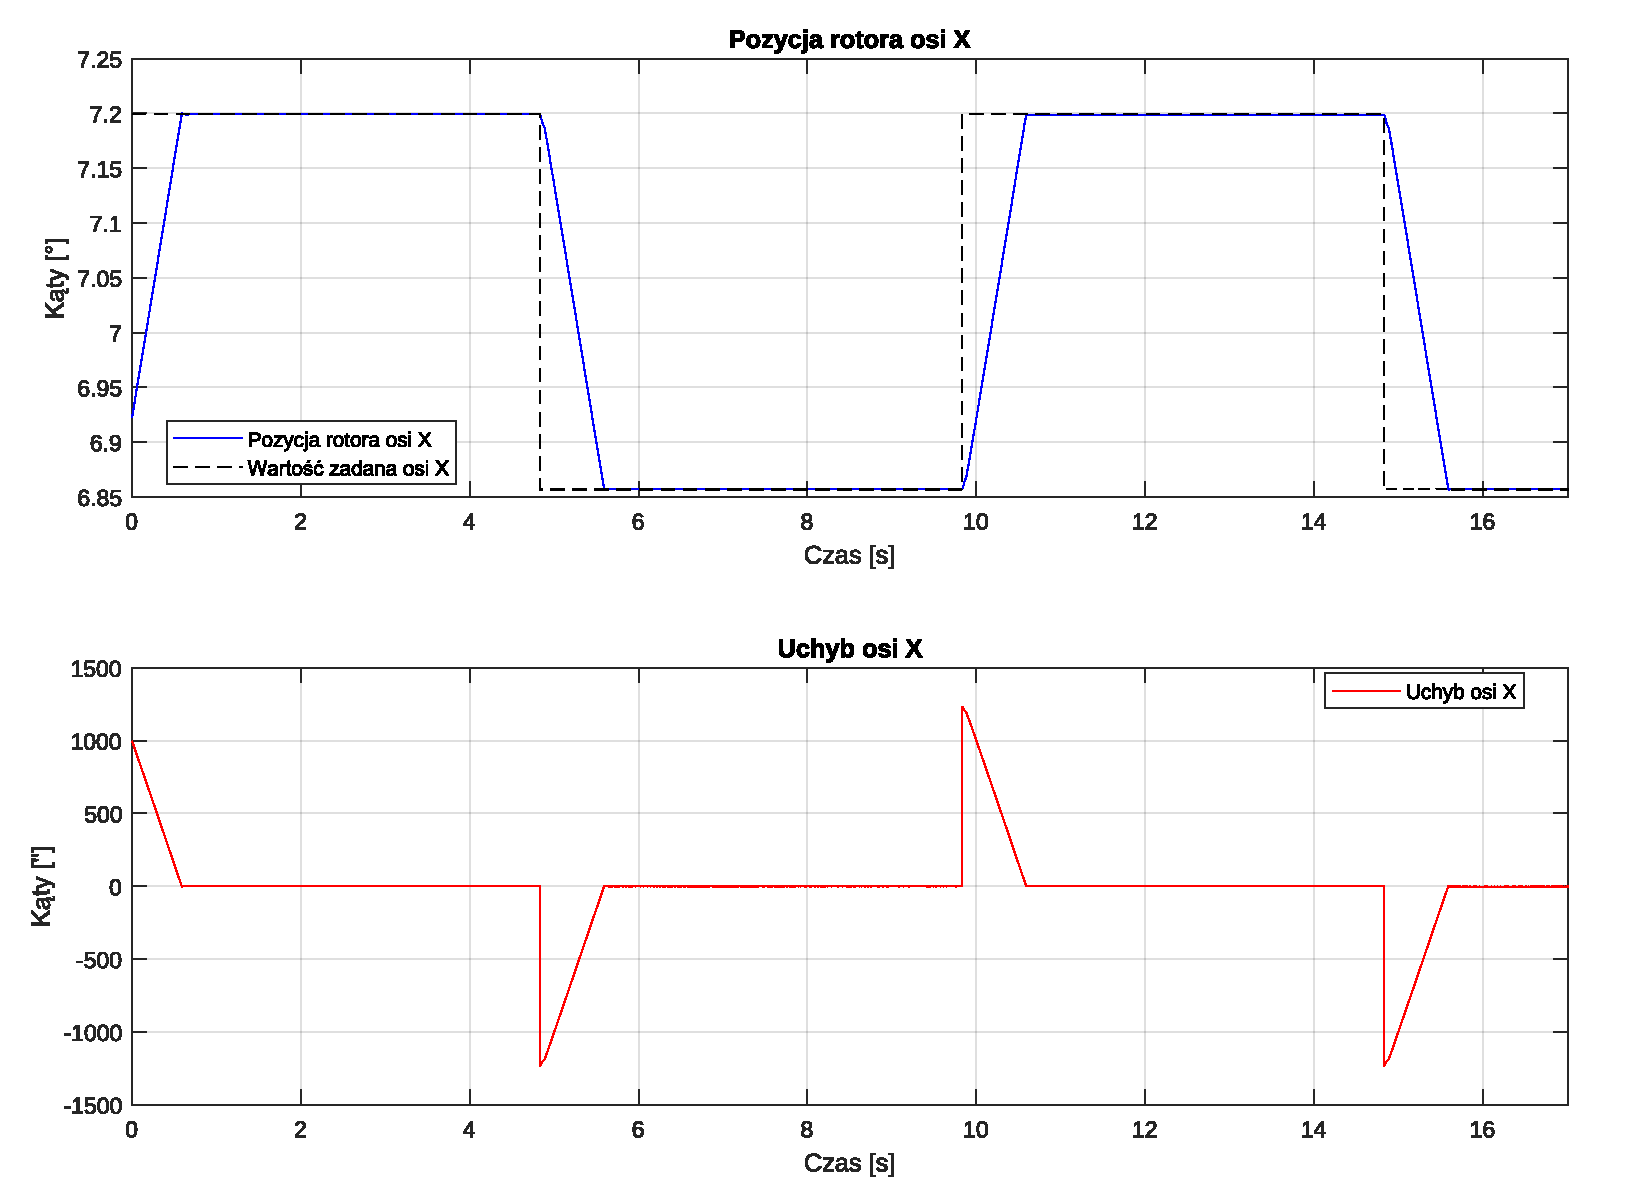
\includegraphics{testy/wykresy_inżynierka/4kY.pdf}}
    \caption{Przebiegi dla sterowania z częstotliwością 4000 Hz na osi X.}
    \label{fig:schemat blokowy pobierania danych2}
\end{figure}


\begin{figure}[H]
    \centering
    \resizebox{12cm}{!}{
    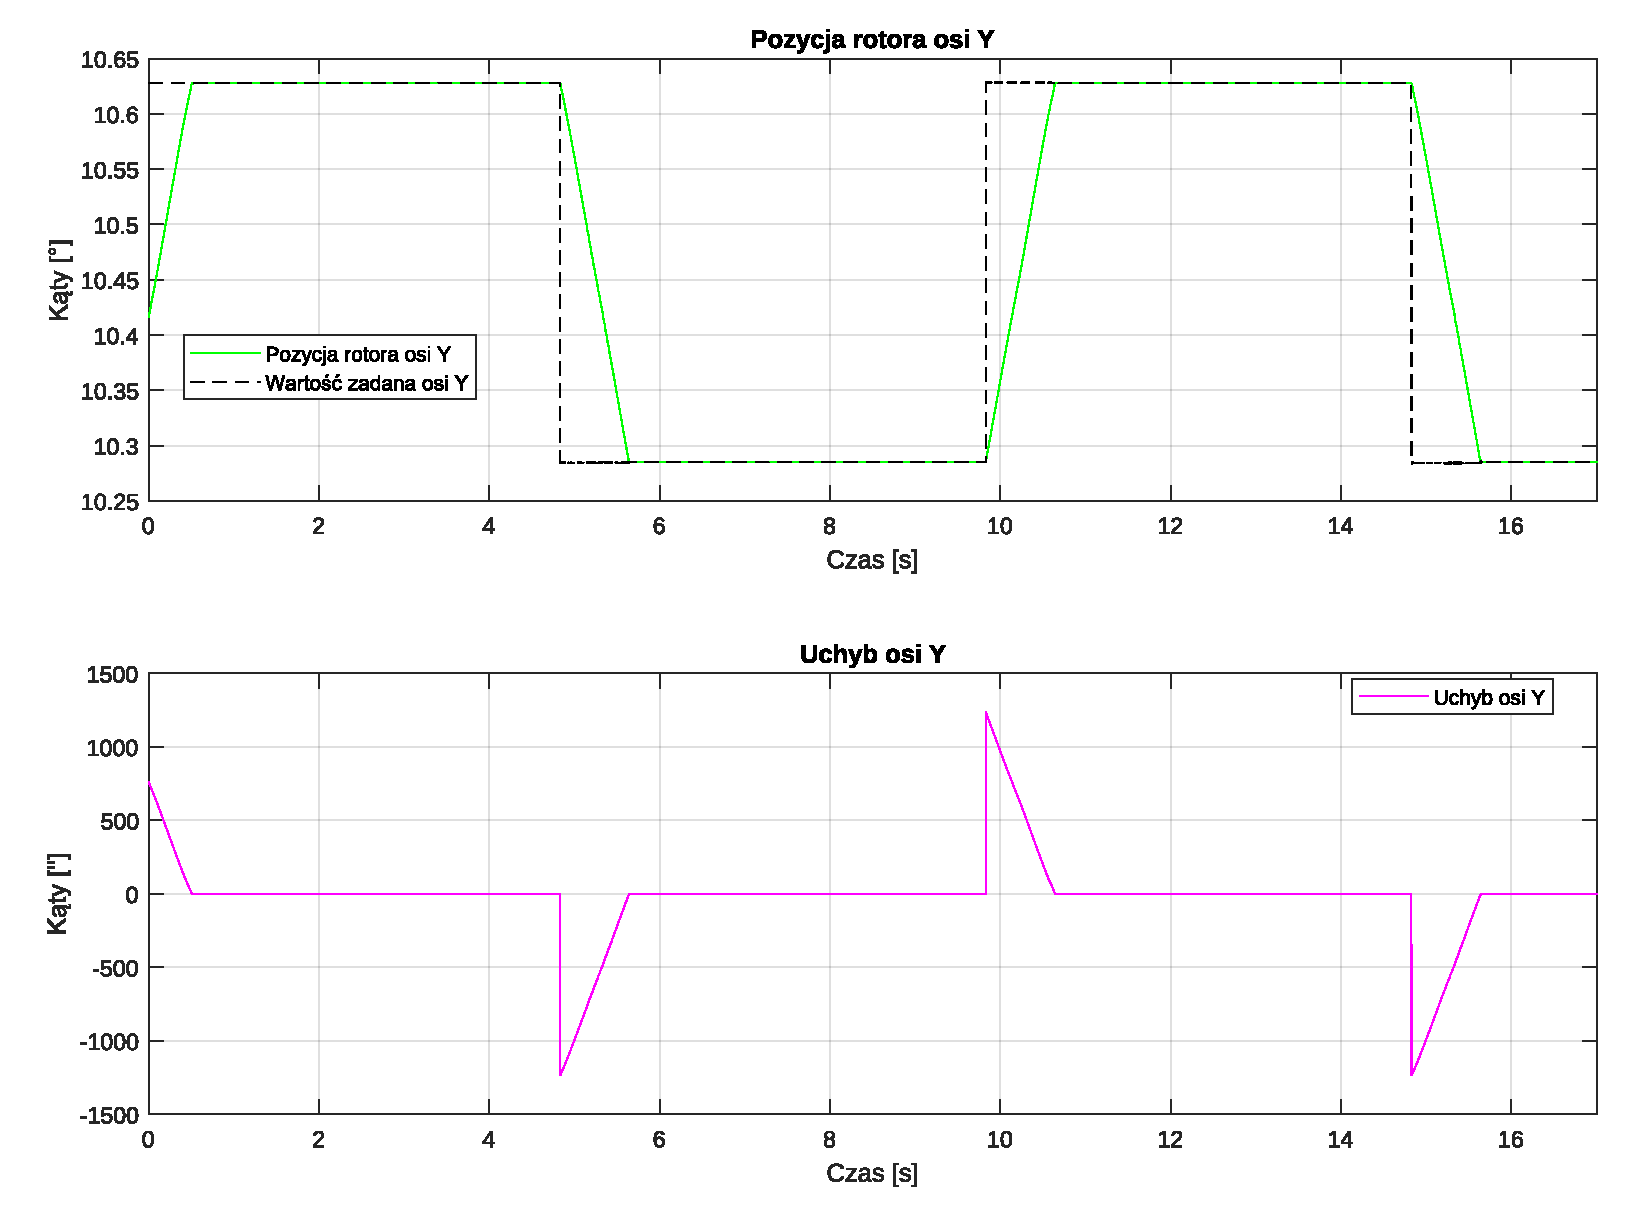
\includegraphics{testy/wykresy_inżynierka/4kX.pdf}}
    \caption{Przebiegi dla sterowania z częstotliwością 4000 Hz na osi Y.}
    \label{fig:schemat blokowy pobierania danych2}
\end{figure}

\begin{figure}[H]
    \centering
    \resizebox{12cm}{!}{
    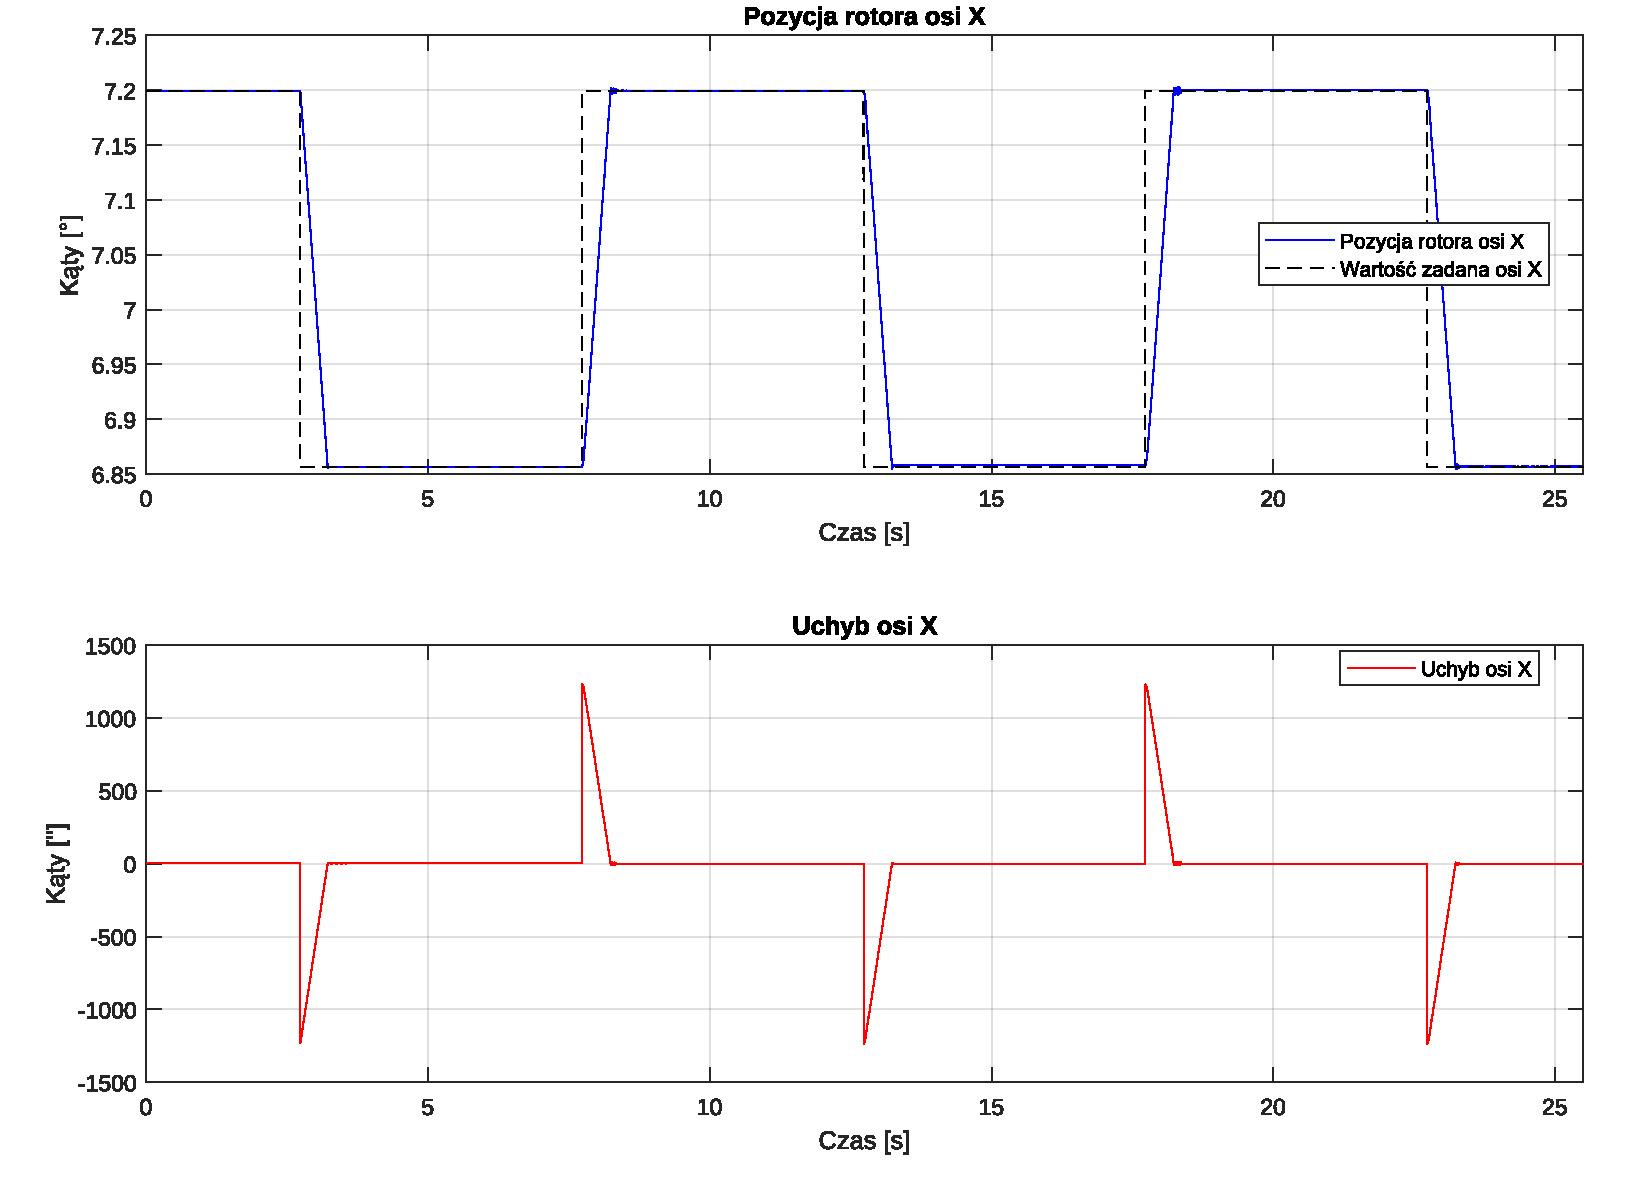
\includegraphics{testy/wykresy_inżynierka/6kX.pdf}}
    \caption{Przebiegi dla sterowania z częstotliwością 6000 Hz na osi X.}
    \label{fig:schemat blokowy pobierania danych2}
\end{figure}


\begin{figure}[H]
    \centering
    \resizebox{12cm}{!}{
    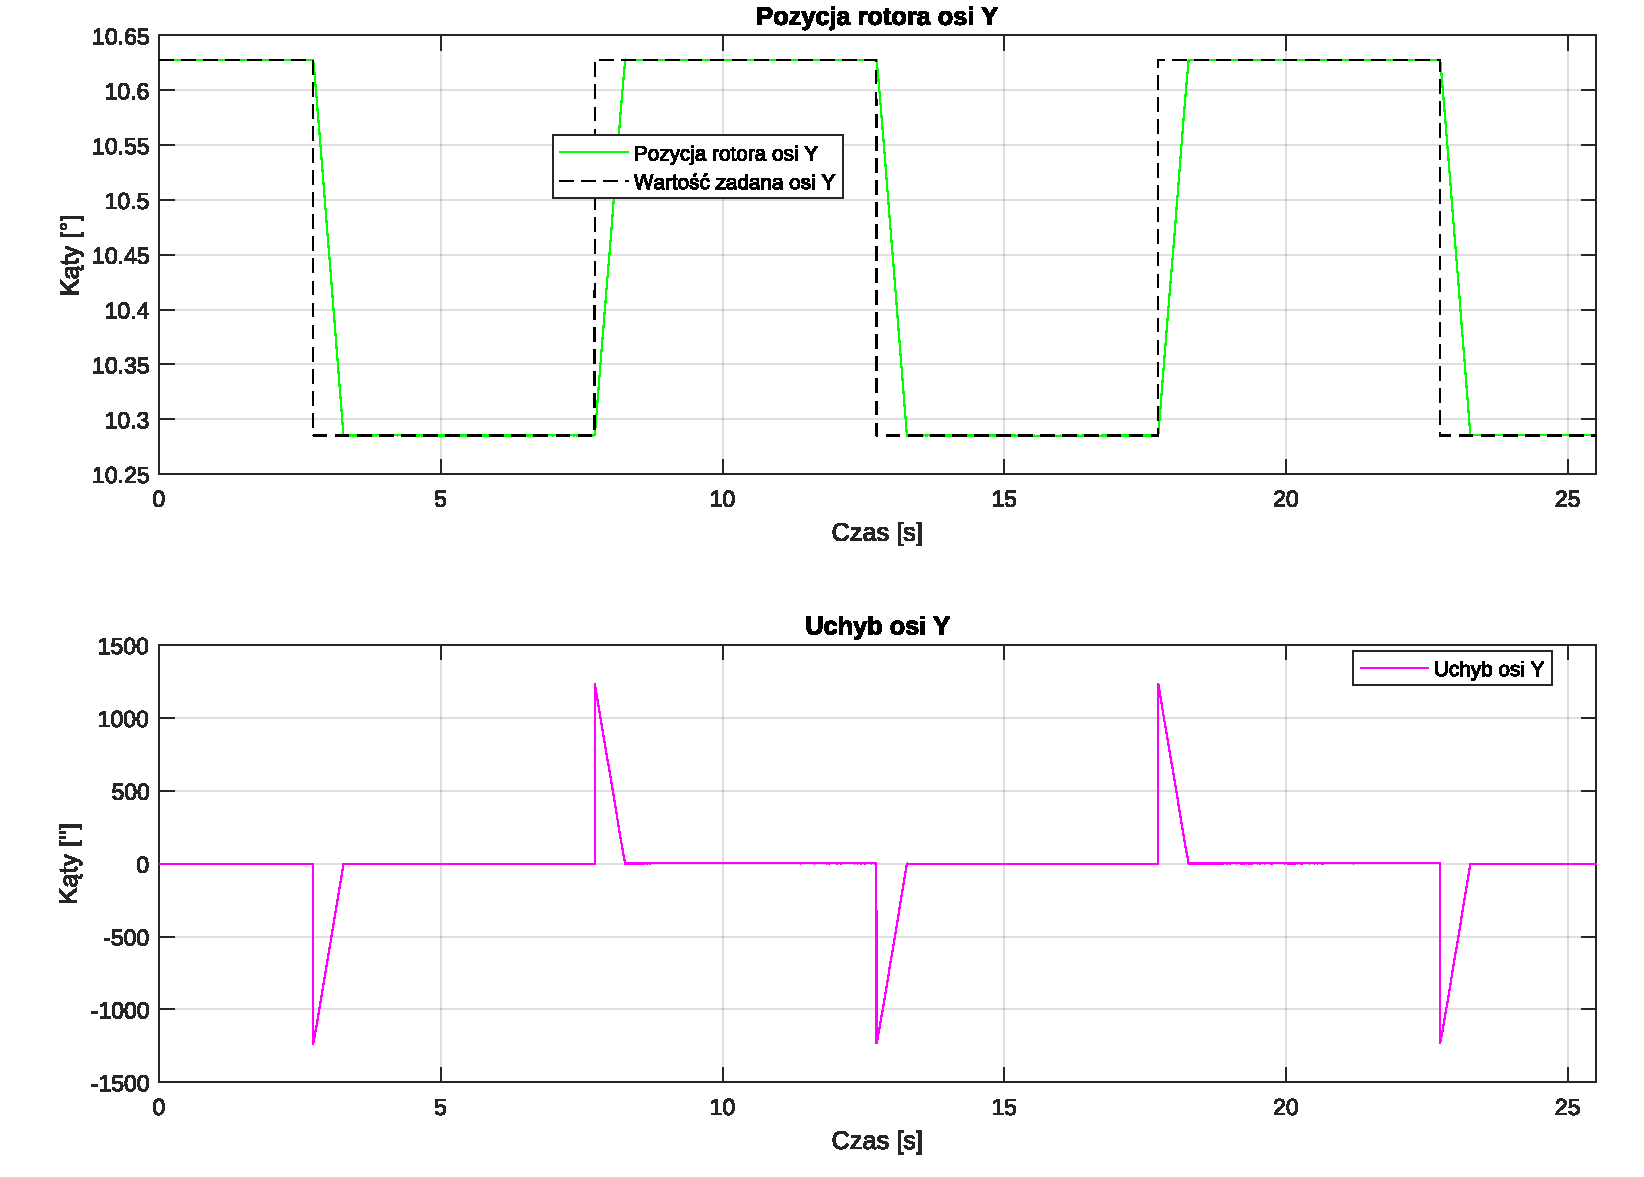
\includegraphics{testy/wykresy_inżynierka/6kY.pdf}}
    \caption{Przebiegi dla sterowania z częstotliwością 6000 Hz na osi Y.}
    \label{fig:schemat blokowy pobierania danych2}
\end{figure}


\begin{figure}[H]
    \centering
    \resizebox{12cm}{!}{
    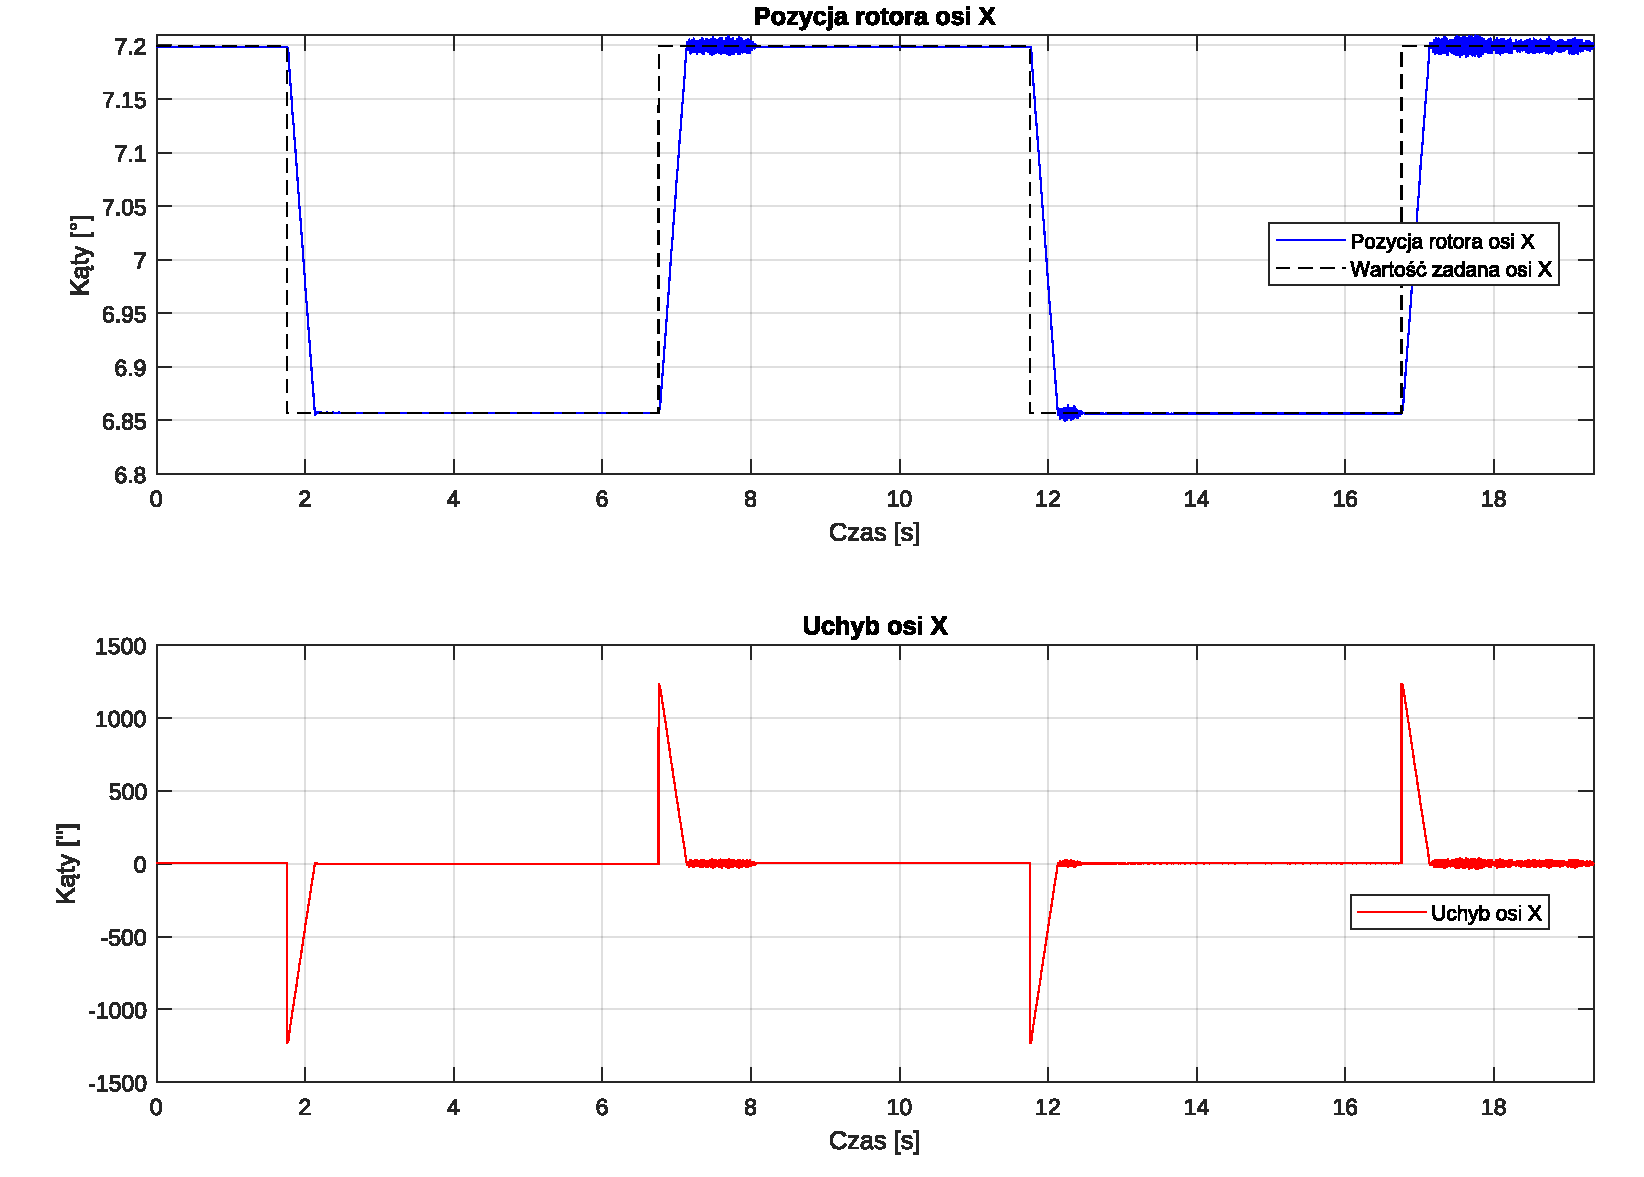
\includegraphics{testy/wykresy_inżynierka/8kX.pdf}}
    \caption{Przebiegi dla sterowania z częstotliwością 8000 Hz na osi X.}
    \label{fig:schemat blokowy pobierania danych2}
\end{figure}


\begin{figure}[H]
    \centering
    \resizebox{12cm}{!}{
    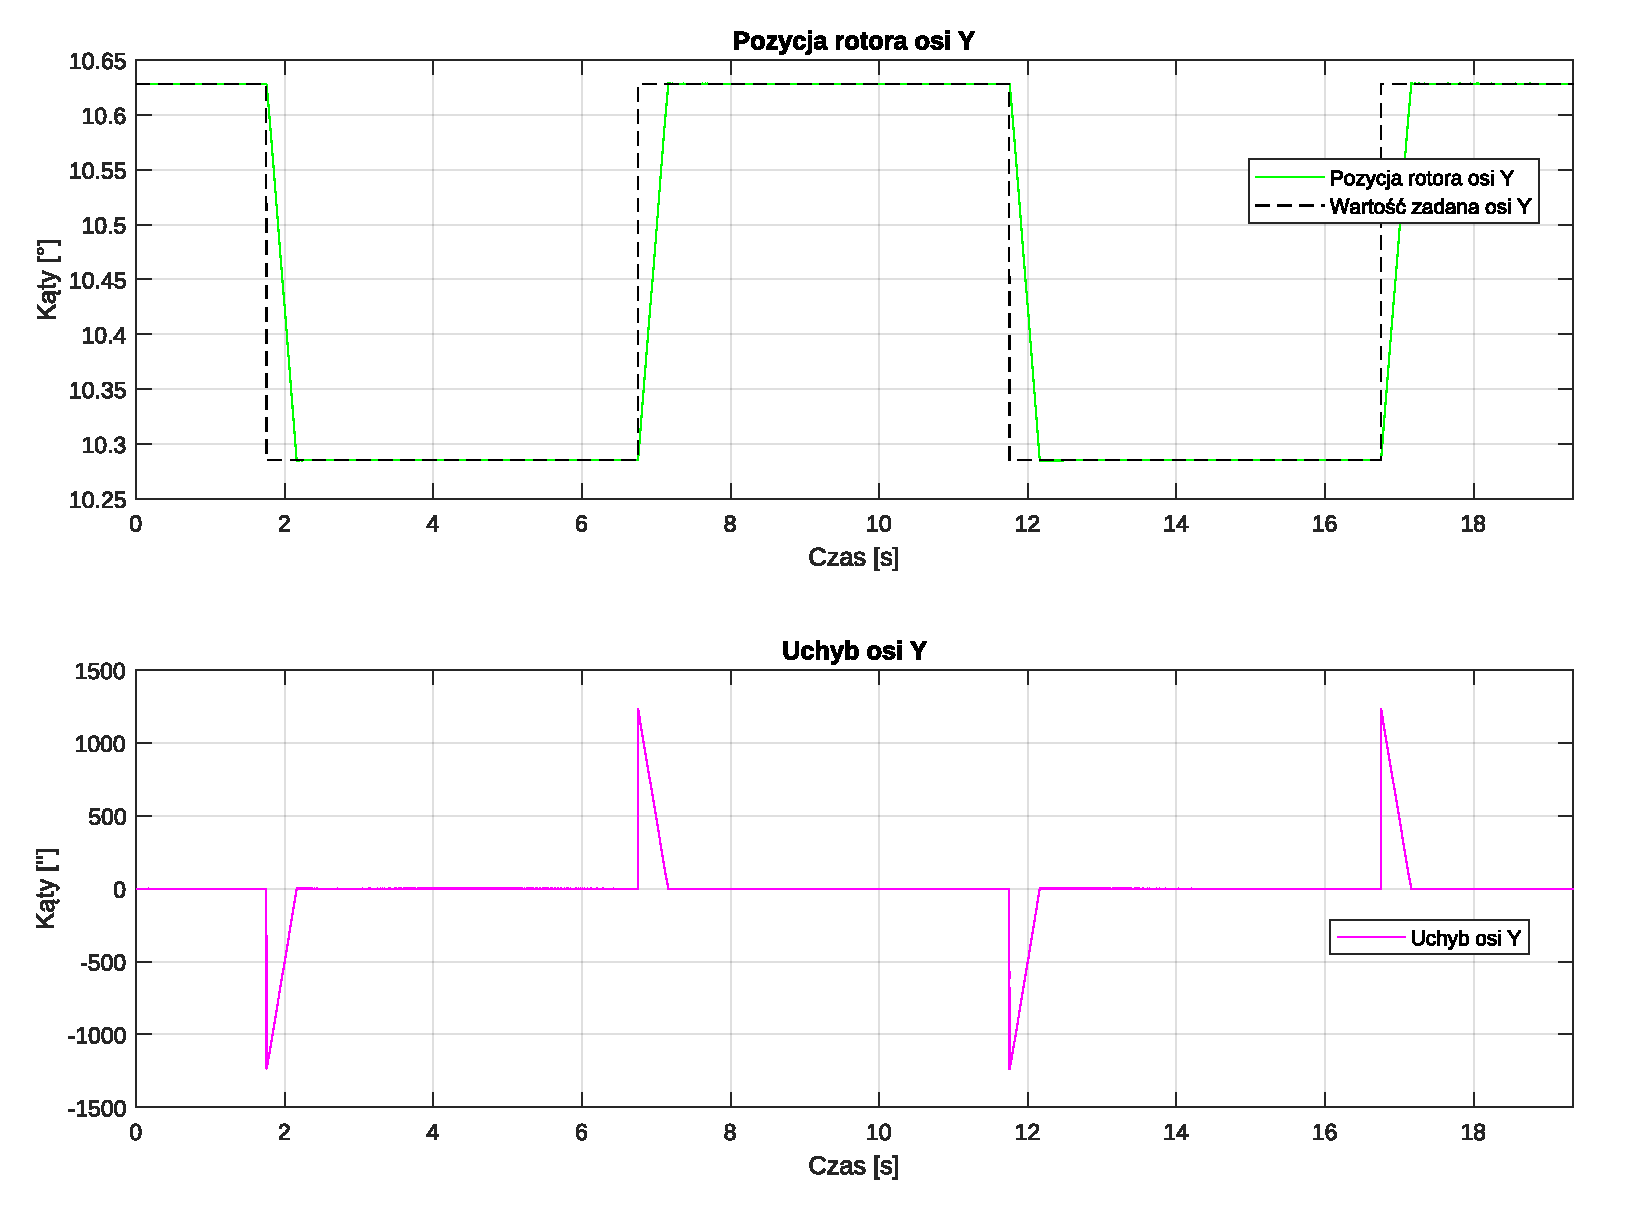
\includegraphics{testy/wykresy_inżynierka/8kY.pdf}}
    \caption{Przebiegi dla sterowania z częstotliwością 8000 Hz na osi Y.}
    \label{fig:schemat blokowy pobierania danych2}
\end{figure}


\begin{figure}[H]
    \centering
    \resizebox{12cm}{!}{
    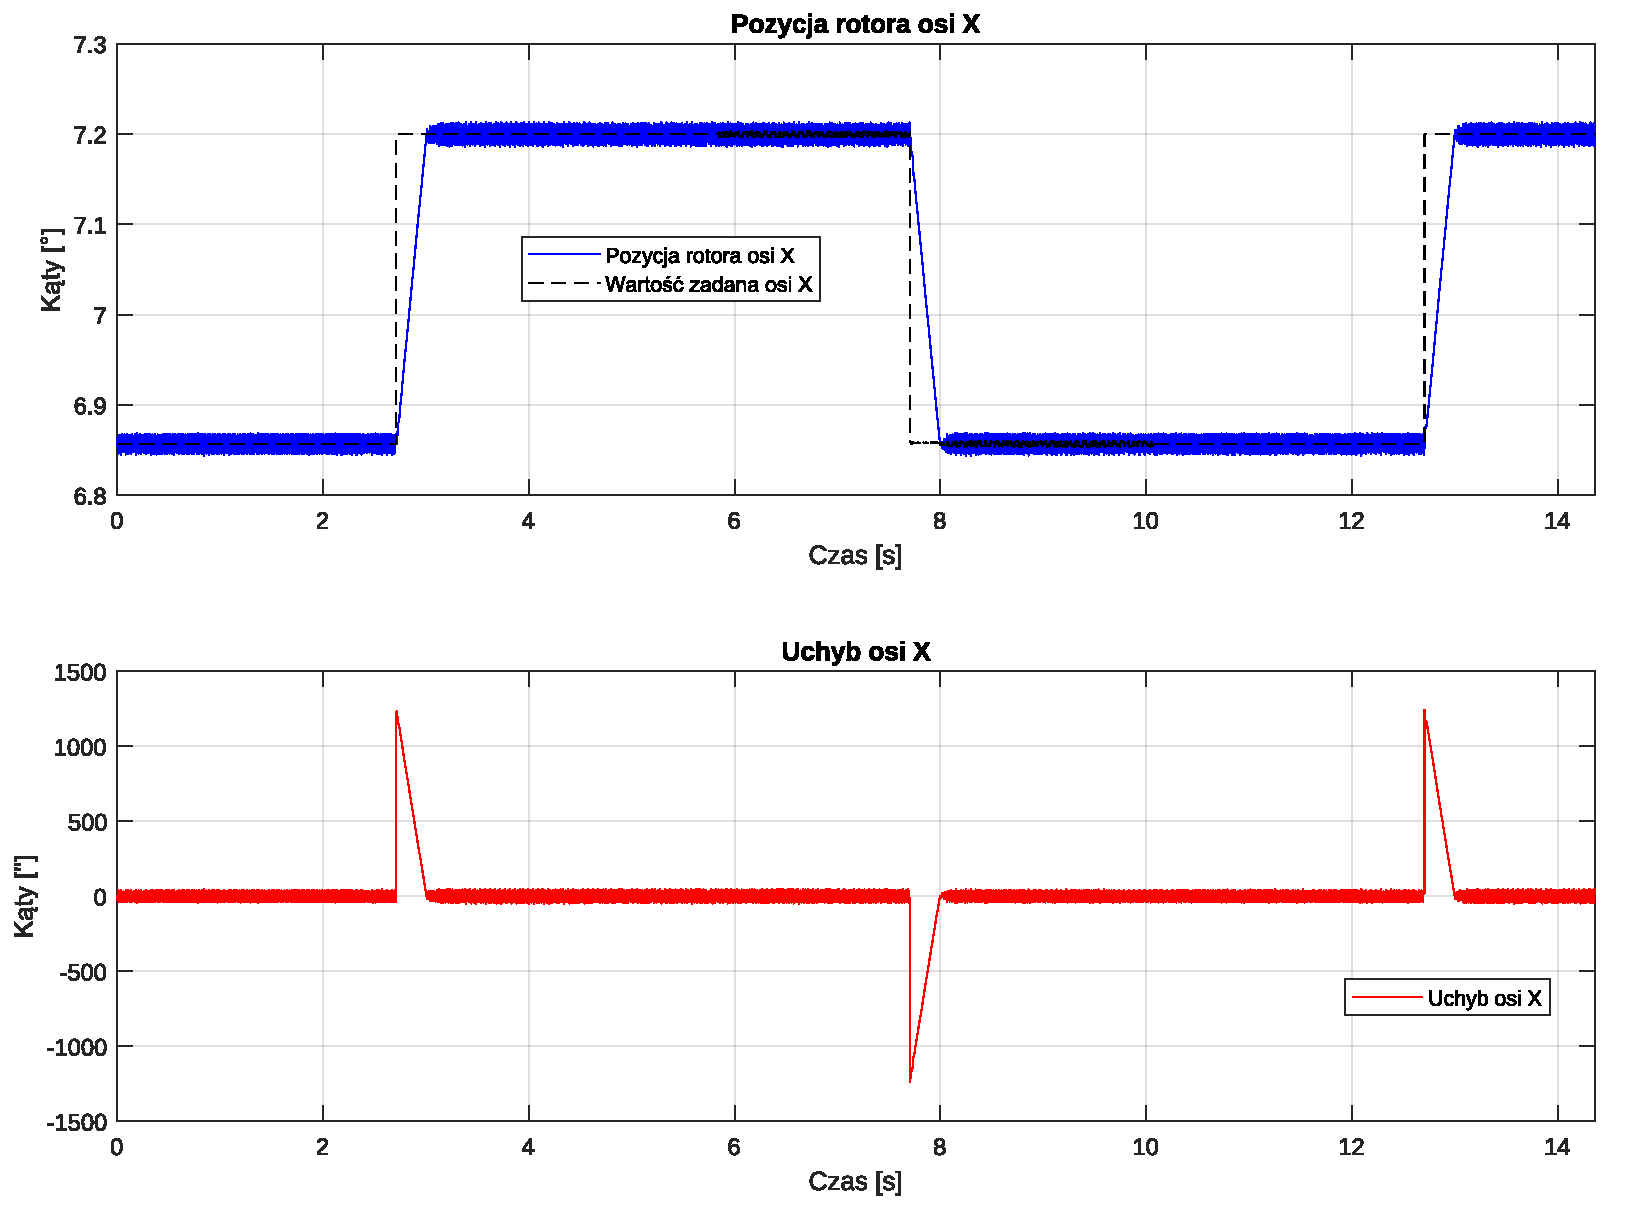
\includegraphics{testy/wykresy_inżynierka/10kX.pdf}}
    \caption{Przebiegi dla sterowania z częstotliwością 10000 Hz na osi X.}
    \label{fig:schemat blokowy pobierania danych2}
\end{figure}


\begin{figure}[H]
    \centering
    \resizebox{12cm}{!}{
    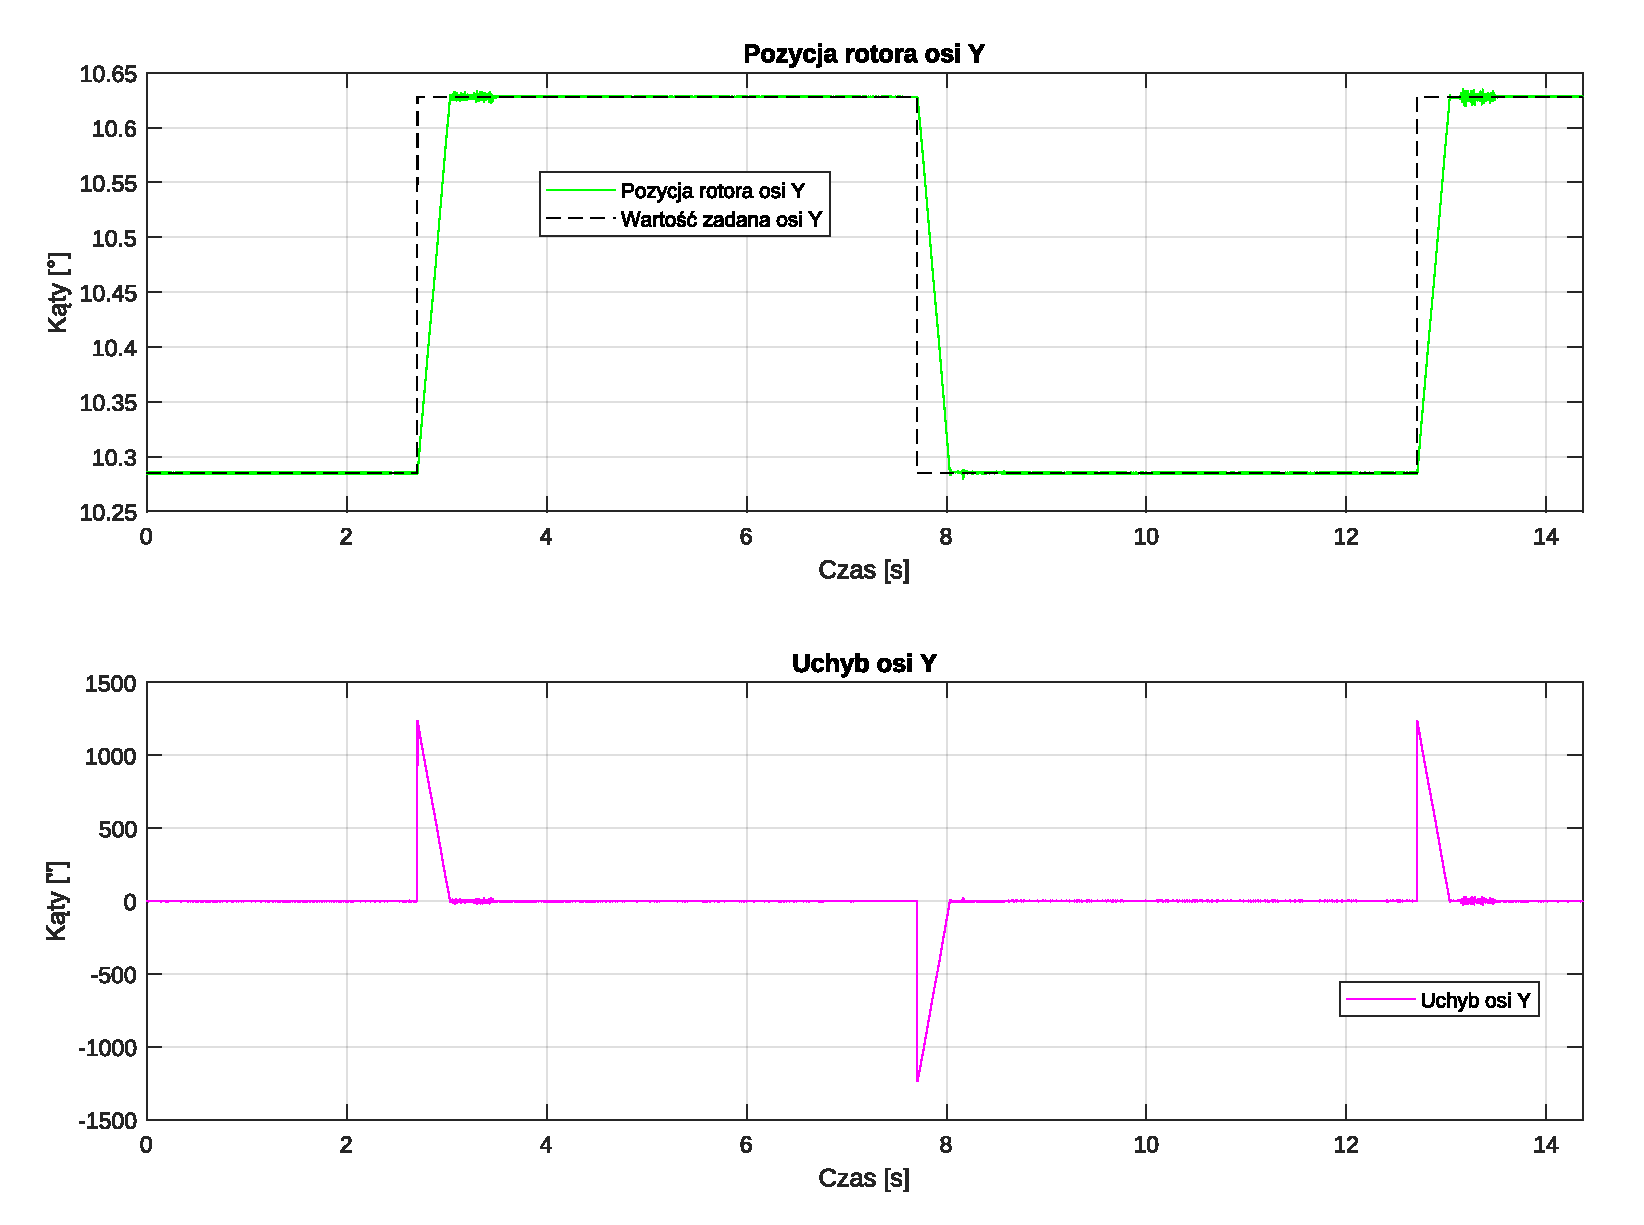
\includegraphics{testy/wykresy_inżynierka/10kY.pdf}}
    \caption{Przebiegi dla sterowania z częstotliwością 10000 Hz na osi Y.}
    \label{fig:schemat blokowy pobierania danych2}
\end{figure}


\begin{figure}[H]
    \centering
    \resizebox{12cm}{!}{
    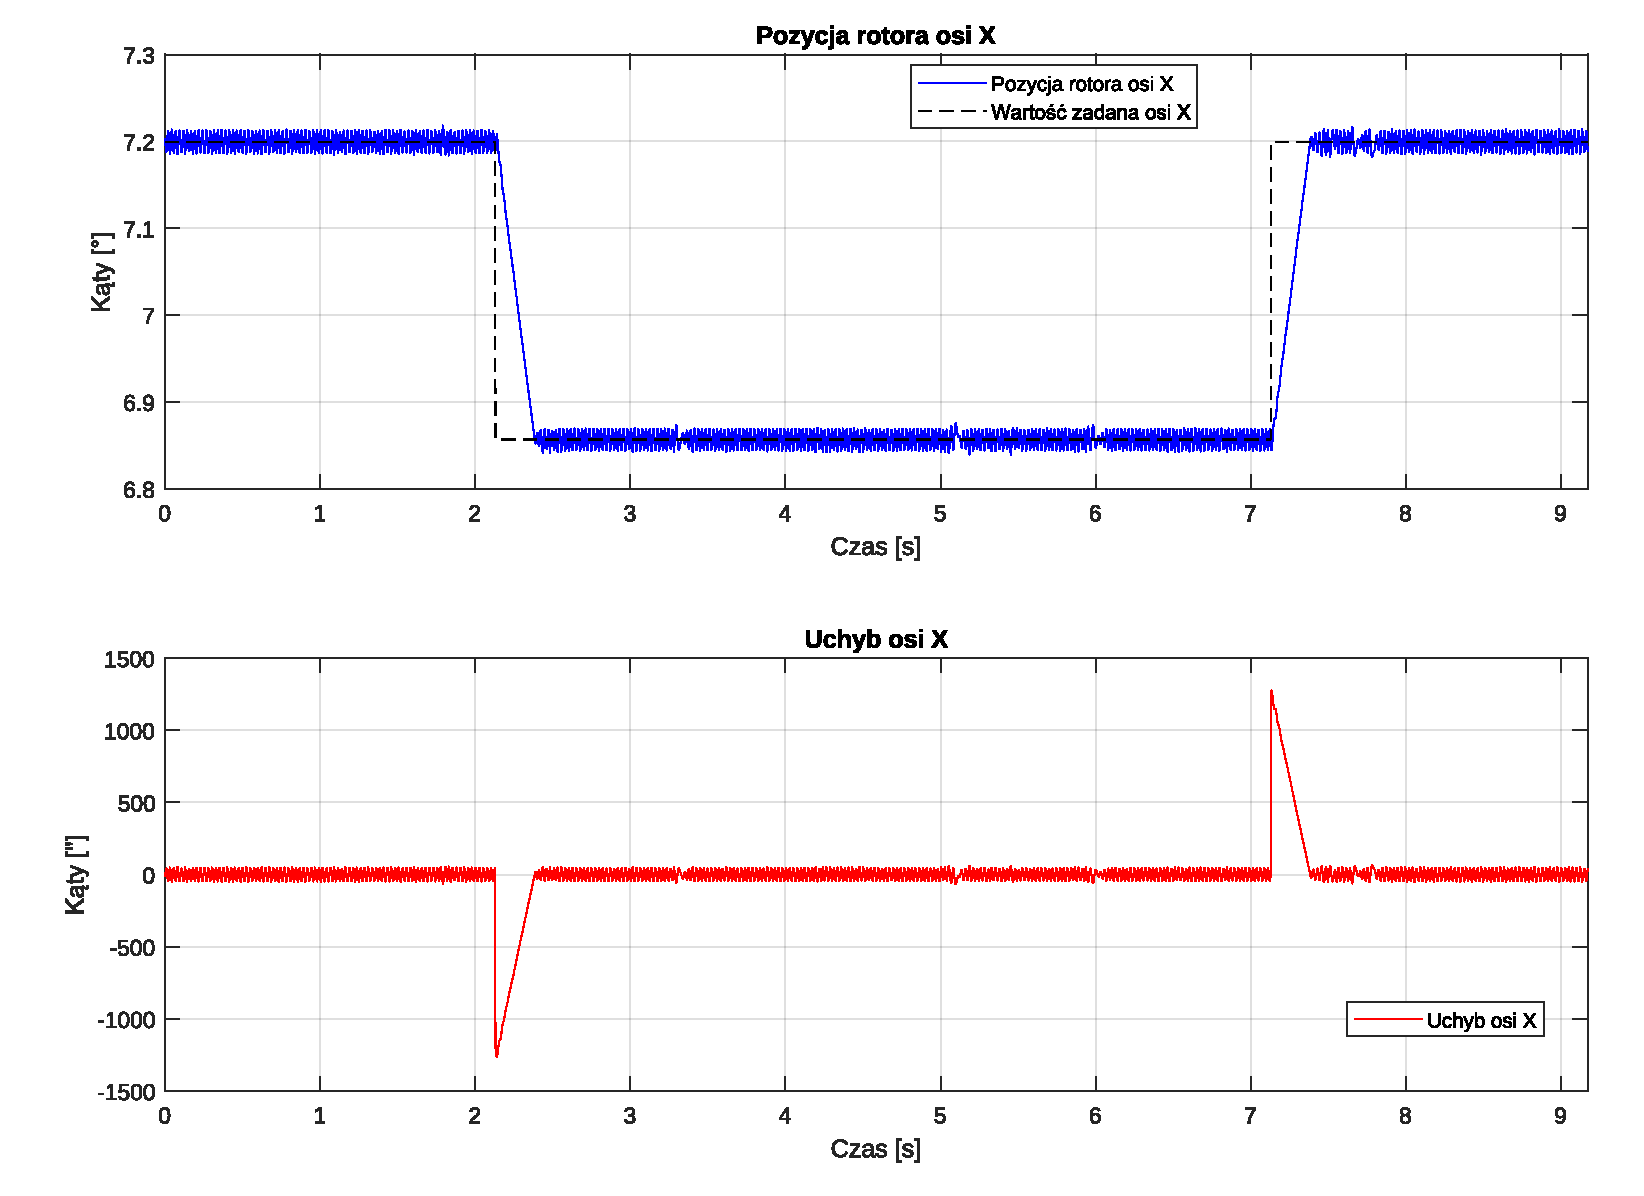
\includegraphics{testy/wykresy_inżynierka/12kX.pdf}}
    \caption{Przebiegi dla sterowania z częstotliwością 12000 Hz na osi X.}
    \label{fig:schemat blokowy pobierania danych2}
\end{figure}


\begin{figure}[H]
    \centering
    \resizebox{12cm}{!}{
    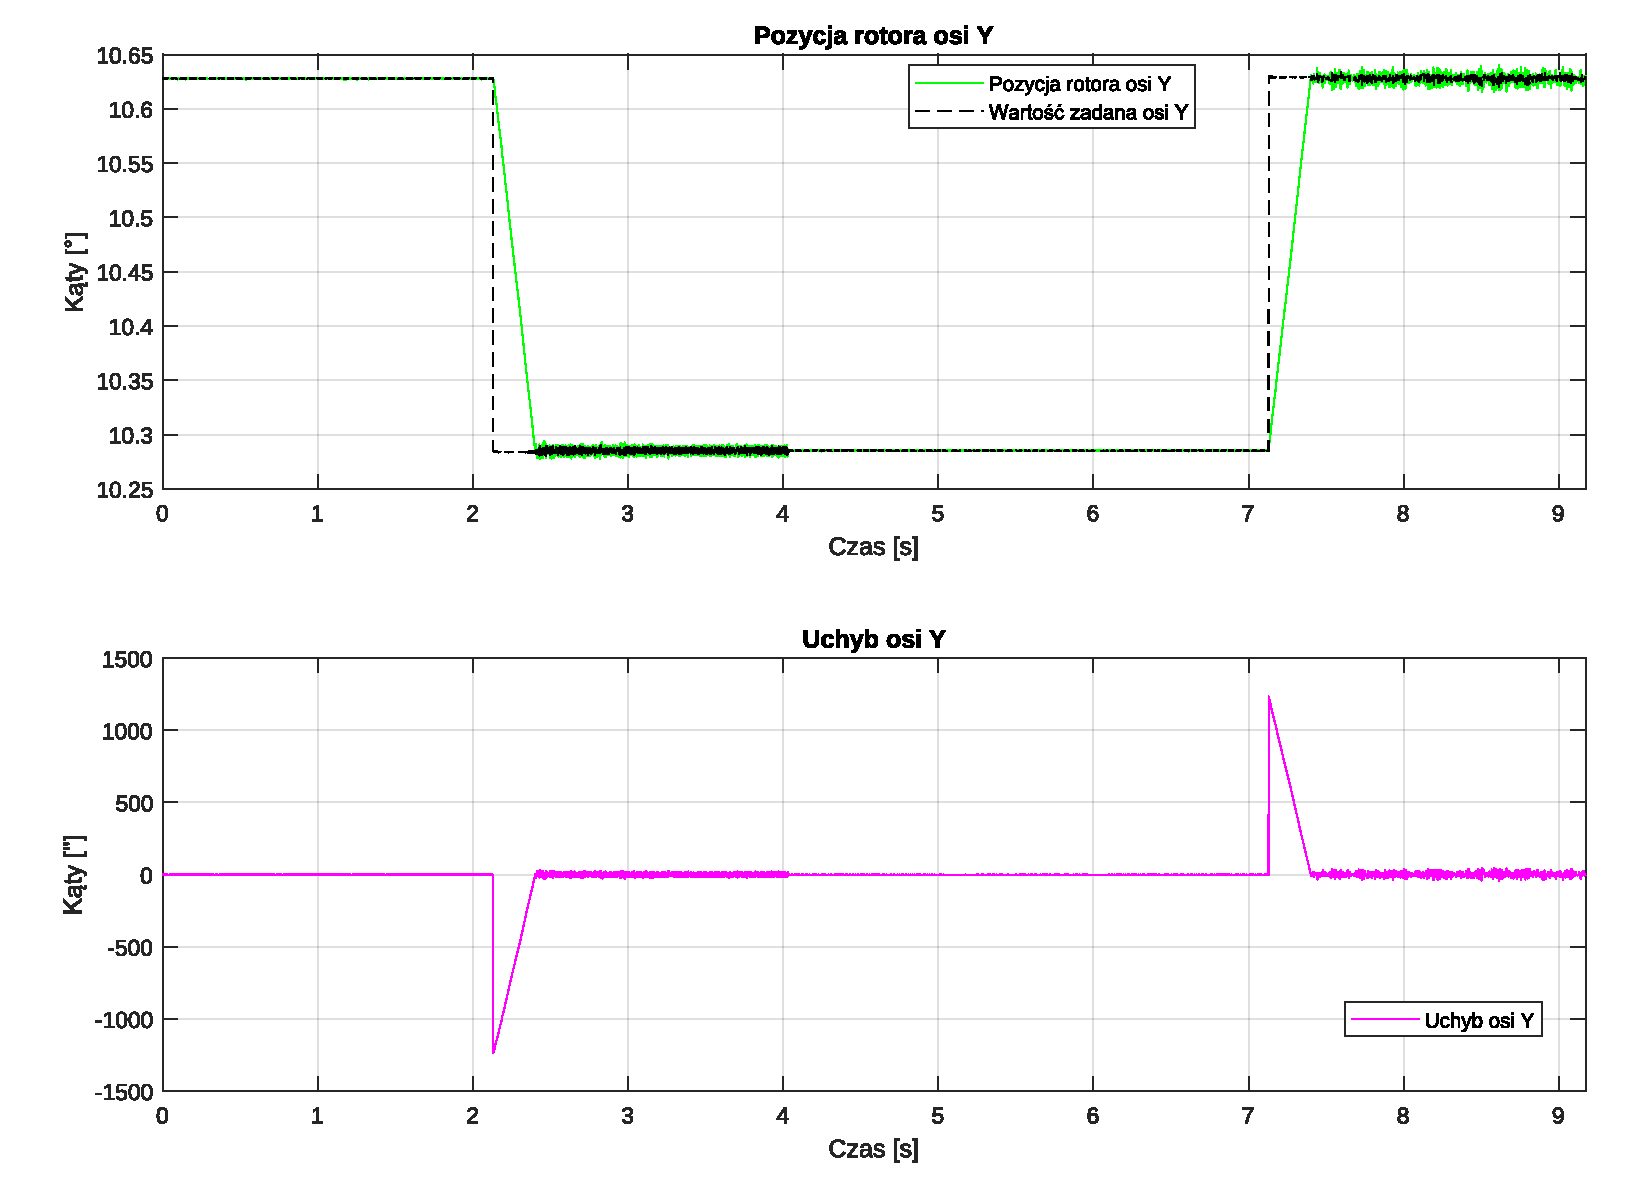
\includegraphics{testy/wykresy_inżynierka/12kY.pdf}}
    \caption{Przebiegi dla sterowania z częstotliwością 12000 Hz na osi Y.}
    \label{fig:schemat blokowy pobierania danych2}
\end{figure}

\vspace{1cm}

Zwiększając częstotliwość sygnału zegarowego podawanego na wejście CLK sterownika silnika można zauważyć, że po osiągnięciu zadanej pozycji system nie zapewniał poprawnej stabilizacji. Częstotliwość impulsów była na tyle duża, że silnik zaczynał gubić kroki, co rozsynchronizowywało pracę systemu i spowodowało zwiększenie błędu pozycjonowania. W takich warunkach odnotowano charakterystyczny dźwięk wydawany przez elementy konstrukcyjne układ napędowego w postaci ,,stukania'' i ,,pukania''. W ten sposób zaobserwowano graniczną wartość częstotliwości sygnału CLK, przy której jeszcze układ regulacji sterujący konstrukcją badanego uchwytu pracuje prawidłowo.

\section{Stany sygnału sterującego silnikiem}

\begin{figure}[H]
    \centering
    \resizebox{12cm}{!}{
    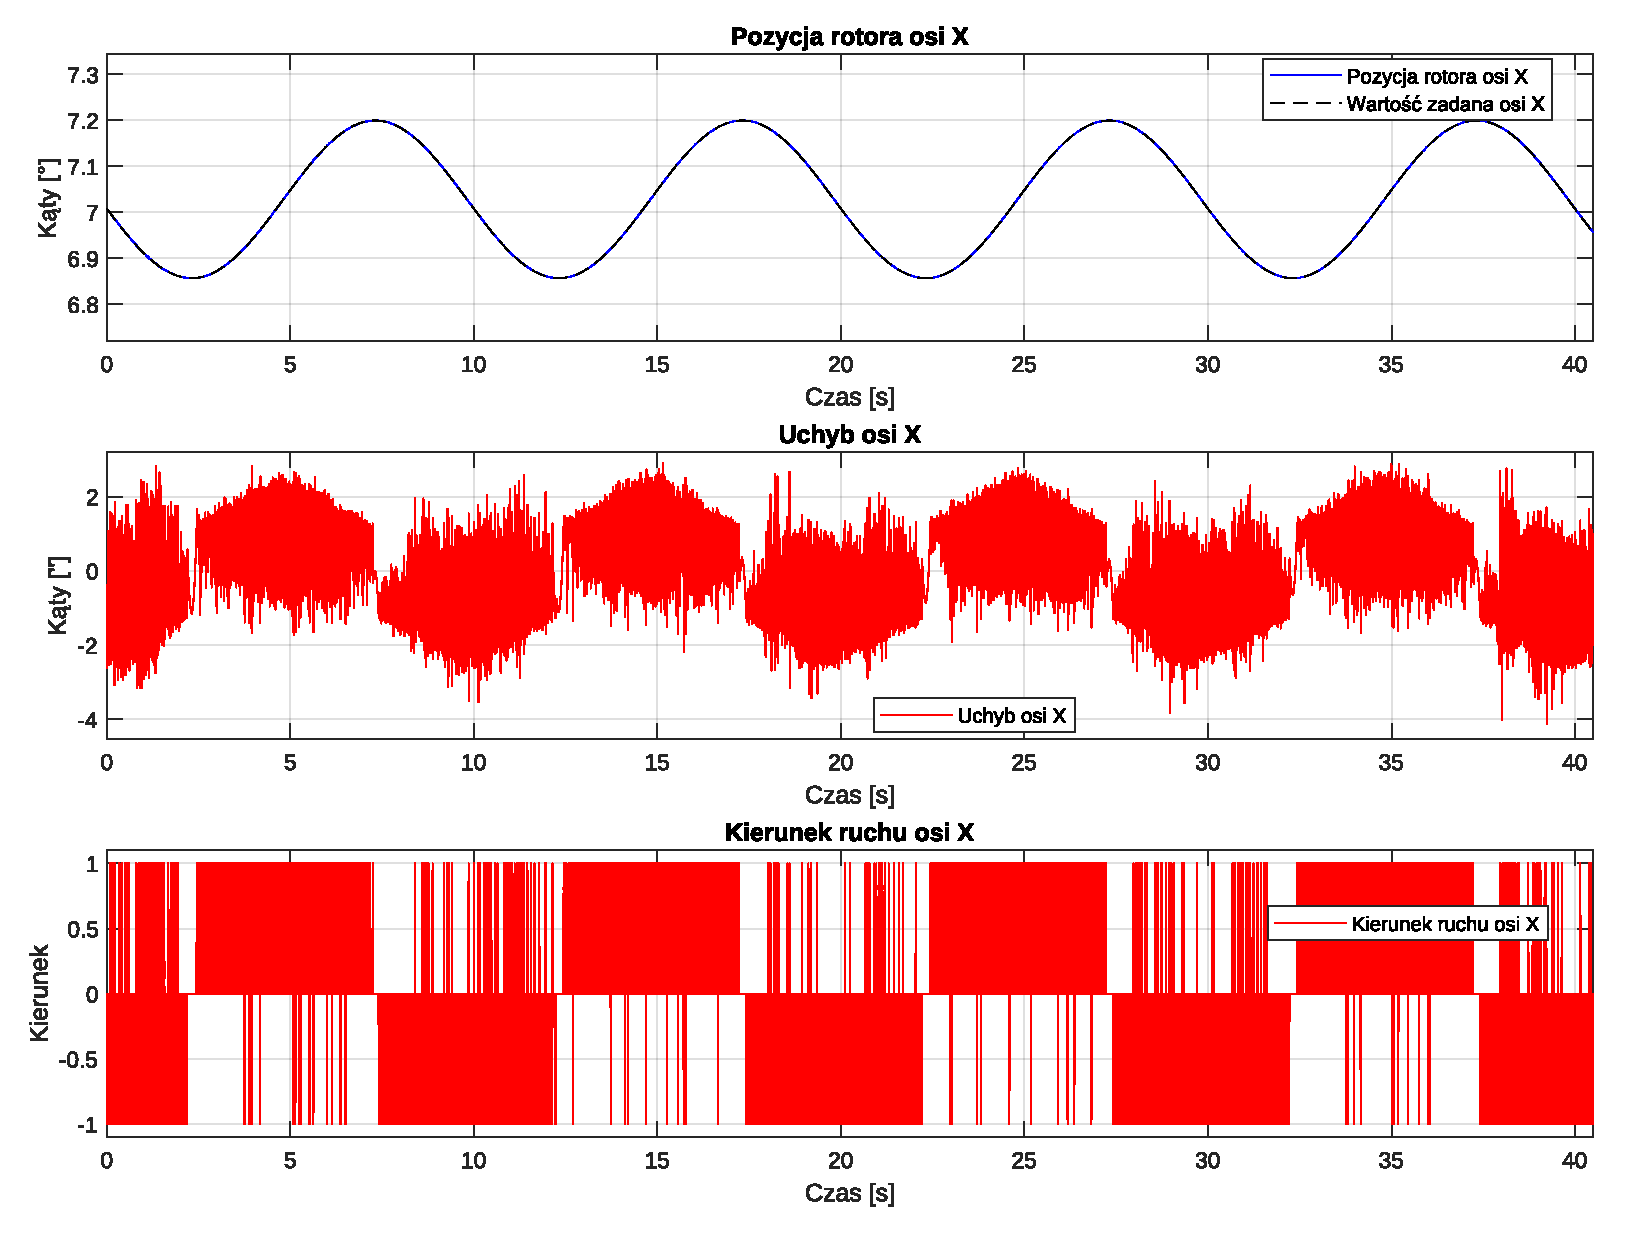
\includegraphics{testy/wykresy_inżynierka/sygnalKierunkowySin10skierunek.pdf}}
    \caption{Przebiegi dla trajektorii sinusoidalnej o okresie 10 sekund na osi X.}
    \label{fig:ster1}
\end{figure}

\begin{figure}[H]
    \centering
    \resizebox{12cm}{!}{
    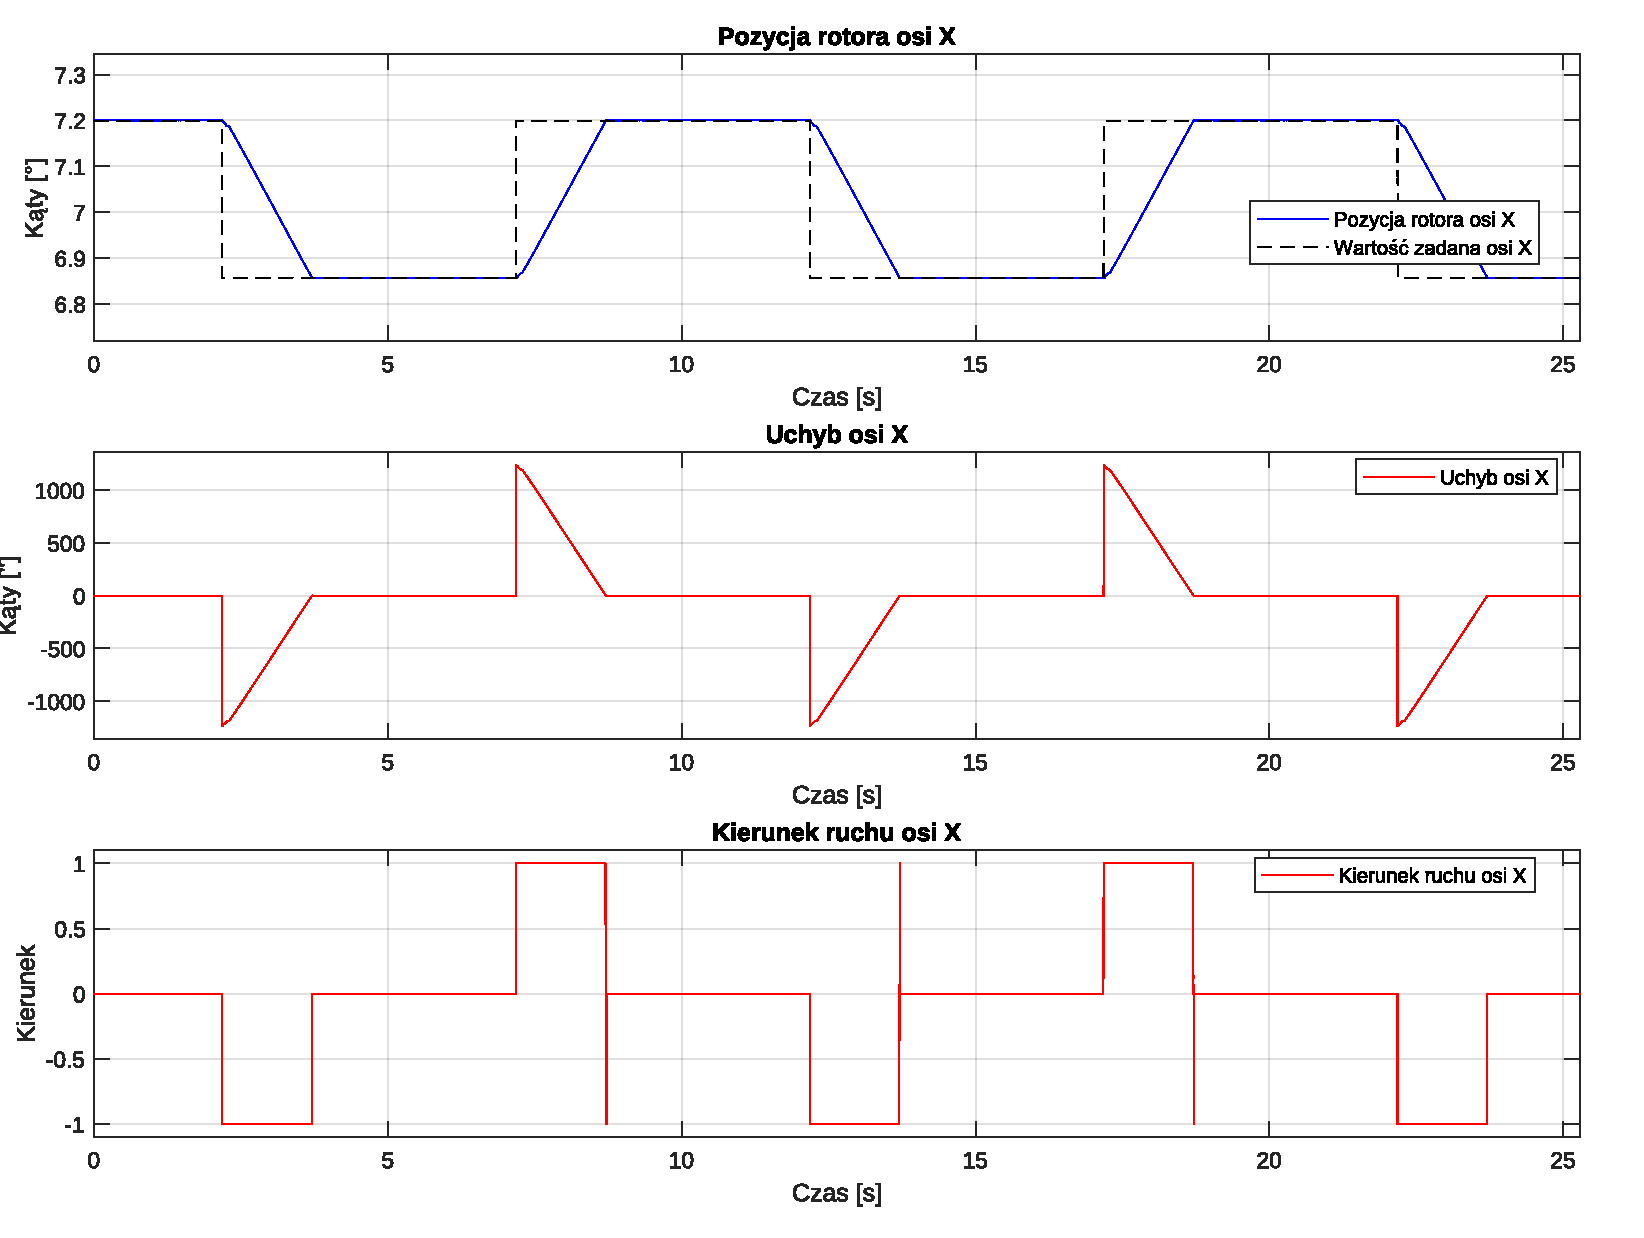
\includegraphics{testy/wykresy_inżynierka/sygnalKierunkowySquarekierunek.pdf}}
    \caption{Przebiegi dla trajektorii prostokątnej o okresie 10 sekund na osi X.}
    \label{fig:ster2}
\end{figure}
Ze względu na ograniczone zasoby mikrokontrolera test z kierunkiem ruchu został wykonany tylko na osi X. Kierunek ruchu osi X na rysunkach \ref{fig:ster1} i \ref{fig:ster2} oznaczono za pomocą następujących wartości liczbowych:
\vspace{0.5cm}
\begin{itemize}
    \item \textbf{1}: Ruch do przodu.
    \item \textbf{0}: Brak ruchu.
    \item \textbf{-1}: Ruch wsteczny.
\end{itemize}
\vspace{0.5cm}
W idealnym przypadku ruch silnika krokowego powinien odbywać się tylko w jednym kierunku w celu uzyskania stałej pozycji zadanej. Wyniki eksperymentalne pokazują, że w praktyce zachodzi potrzeba wielokrotnych zmian kierunku z uwagi na występujące oscylacje, szumy pomiarowe oraz użytą trajektorie referencyjną. Z powodu braku histerezy widoczne są szybkie zmiany kierunku na granicach wyznaczanych przez strefę nieczułości. Zjawisko to jest szczególnie widoczne przy użyciu trajektorii prostokątnej. Gdy układ osiąga pozycję zadaną, następuje korekta, a po niej system się stabilizuje i ruch ustaje.

% \chapter{Wykorzystane programy i środowiska programistyczne w pracy inżynierskiej}
% \section{Git}
Do kontroli wersji aplikacji webowej i aplikacji na STM32 został wybrany Git \cite{Git}. Git jest systemem kontroli wersji, który umożliwia zarządzanie historią zmian w projekcie. Jest niezwykle przydatny w celu podejrzenia wszelkich zmian pomiędzy commit'ami.
\subsection{Podstawowe cechy Git}
Git działa w oparciu o repozytorium, w którym przechowywane są wszystkie wersje plików. Repozytorium może być zarówno lokalne jak i online, w tym przypadku wybrano repozytorium online na portalu GitHub, ponieważ ułatwiło to pracę w zespole jak i na wielu urządzeniach. Główne narzędzia dostępne w Git, które ułatwiają pracę:
\begin{enumerate}
    \item \textbf{Commit:} zapisanie zmian plików do historii. Commit powinien również zawierać opis, który obrazuje dokonane zmiany.
    \item \textbf{Branch (gałąź):} wersja projektu rozwijana równolegle z innymi. Dzięki gałęziom możemy rozwijać różne funkcje równocześnie bez zakłócania pracy nad główną wersją projektu. Jest to dobra praktyka w trakcie rozwijania nowej funkcjonalności, ponieważ nie dodajemy niestabilnych elementów na główny branch. Nazwą głównego brancha na portalu GitHub jest \textit{main}.
    \item \textbf{Merge:} połączenie zmian z jednej gałęzi z inną. Pozwala na przeniesienie efektów pracy z jednej gałęzi do głównej lub między innymi gałęziami. Było to przydatne w celu dodania 
 skończonych i sprawdzonych nowych funkcjonalności na główny branch.
    \item \textbf{Tags (tagi):} to etykiety przypisywane do danej wersji projektu. Tagi są przydatne do szybkiego nawigowania między wersjami projektu. Tagi zostały przede wszystkim wykorzystane do tworzenia stabilnych wersji, które przyczyniły się do testowania czy nowe oprogramowanie wpłynęło na negatywne działanie całego projektu.
\end{enumerate}
\subsection{Praca sieciowa}
Git przechowuje całą historię zmian w plikach w postaci serii commit'ów i przechowuje zmiany w postaci zestawu różnic (ang. \textit{diff}) między kolejnymi wersjami plików. Cała historia znajduje się na serwerze, którą można pobrać na lokalny komputer i pracować bez połączenia z siecią. Połączenie z siecią jest potrzebne do pobrania najnowszej wersji projektu \textit{git pull} lub \textit{git fetch} i do wysyłania własnych zmian \textit{git push}.
\subsection{Podsumowanie}
Git to przydatne narzędzie, które wprowadza porządek do projektu. Ułatwia kontrole nad wersjami aplikacji i umożliwia równoległą pracę nad wieloma funkcjonalnościami oraz zapewnia bezpieczeństwo dzięki historii zmian. W przypadku problematycznych nowych funkcjonalności można się cofnąć do poprzedniej stabilnej wersji.


\section{Virtual DOM}
\label{section:Virtual DOM}

Jest to technologia wykorzystywana przez rózne biblioteki i frameworki (w tym przez React) do efektywnego zarządzania aktualizacjami interfesju w aplikacjach webowych. DOM to Document Object Model, czyli obiektowy model dokumentu. Jego struktura to drzewo, która reprezentuje elementy HTML na aplikacji. Każda zmiana w rzeczywistym DOM jest kosztowna względem wydajności, dlatego Virtual DOM jest niezwykle przydatne w tym przypadku, ponieważ co 200ms ładuje się 800 nowych próbek na wykresy.
\subsection{Działanie Virtual DOM}
Virtual DOM jest uproszczoną wersją drzewa DOM, która jest tworzona przez React i utrzymywana w pamięci. Umożliwia to minimalizowanie liczby bezpośrednich operacji na rzeczywistym DOM. Po każdej zmianie stanu aplikacji Virtual DOM jest porównywany z jego poprzednią wersją, a następnie React dokonuje niezbędnych aktualizacji rzeczywistego DOM, co przekłada się na lepszą optymalizację.

\subsection{Zalety Virtual DOM}
Virtual DOM posiada kluczowe korzyści, które w efektywny sposób przyczyniają się di wydajności i łatwości zarządzania aplikacjami:

\begin{enumerate}
    \item \textbf{Wyższa wydajność}: dzięki aktualizacjom dokonywanym najpierw Virtual DOM, a następnie w rzeczywistym DOM, liczba zasobożernych operacji jest w znacznym stopniu redukowana.
    \item \textbf{Optymalizacja zmian}: proces porównywania zmian w stanie aplikacji pozwala Reactowi dokonywania tylko niezbędnych zmian w rzeczywistym DOM, co znacząco wpływa na wydajność aplikacji. Gdyby za każdym razem stare próbki miały się przeładowywać, to nie byłoby możliwe z dużą częstotliwością przetwarzać dane na wykresach.
    \item \textbf{Prostsze zarządzanie stanem}: dzięki Virtual DOM React może efektywnie zarządzać stanem komponentów, ponieważ aktualizację są dokonywane w myśl sposobu deklaratywywnego, a nie imperatywnego.
    \item \textbf{Modularność}: Virtual DOM umożliwia tworzenie aplikacji z małych i izolowanych komponentów, które w przypadku zmiany stanu będą się aktualizować bez wpływu na inne części aplikacji.
\end{enumerate}
% \subsection{react-plotlyjs}
% React-plotly.js to biblioteka umożliwiająca integrację biblioteki Plotly.js z Reactem. Służy ona do wizualizacji danych z aplikacjami stworzonymi w React. Umożliwia ona tworzenie zaawansowanych i interaktywnych wykresów, które można w bardzo prosty sposób zarządzać i dynamicznie zmieniać wyświetlane dane na wykresie za pomocą React.
% \subsection{Jak działa react-plotlyjs?}
% React Plotly.js oferuje komponent Reactowy, który opiera się na Plotly.js. Wykorzystuje właściwości props do definiowania danych, wyglądu i funkcji interaktywnych wykresów. Dzięki tym narzędziom można w prosty sposób sposób zmieniać dane jak i wygląd wykresów. W aplikacji jest możliwość zmiany jednostek, wspomniana wcześniej biblioteka w prosty sposób umożliwia modyfikacji opisów osi jak i zamianę danych na wykresie.
% \subsection{Zalety react-plotlyjs}
% \begin{enumerate}
%     \item \textbf{Interaktywność:} Zapewnia interaktywne funkcje, takie jak powiększanie, przesuwanie, tooltipy i zapis wykresu.
%     \item \textbf{Integracja z React:} Dzięki komponentowi plotly.js można w prosty sposób zarządzać dynamicznie stanem wykresów. W tym przypadku cały czas wykresy są aktualizowane z aktualną pozycją rotorów jak i uchybem.
%     \item \textbf{Wydajność:} W aplikacji jest wgrywanych, na pojedyńczy wykres, co sekundę aż 1 000 nowych próbek, co w znaczny sposób obciąża aplikację. Jednym z ze sposobów polepszenia wydajności jest zastosowanie WebGL, poprzez typ wykresu scatterg, co znacząco polepsza wydajność przy renderowaniu wykresów.
%     \item \textbf{Eksport danych:} Umożliwia eskport wykresów w formacie PNG.
% \end{enumerate}
% Standardowe wykresy rozproszone w Plotly.js (\textit{scatter}) wykorzystują SVG do renderowania punktów i linii, co jest efektywne dla małych i średnich zbiorów danych. Na wykresach jest ładowana duża ilość próbek, która może być liczona w milionach przez co w tym przypadku renderowanie za pomocą SVG jest niewydajne. W takich przypadkach wykorzystuje się scattergl, który wykorzystuje WebGL.
% Jednym z minusów scattergl jest mniejsza ostrość, ponieważ wykres nie jest renderowany wektorowo.

\section{cJSON}
\label{section:cJSON}
cJSON \cite{cJSON} jest lekką biblioteką napisaną w języku C, która służy do obsługi danych w formacie JSON (JavaScript Object Notation). JSON jest jednym z najbardziej popularnych formatów wymiany danych, który jest szeroko stosowany. Swojej popularności zawdzięcza prostocie i czytelności. Powyższa biblioteka umożliwia parsowanie, tworzenie i modyfikowanie struktur JSON w wydajny sposób z niskim zużyciem zasobów procesora. Alternatywną do JSON jest XML, ale zajmuje o wiele więcej pamięci, która jest kluczowa dla mikroprocesorów.
\subsection{Zalety cJSON}
\begin{enumerate}
    \item \textbf{Lekkość:} cJSON jest małą biblioteką, na licencji MIT, co czyni ją idealną do zastosowania w systemach wbudowanych o ograniczonych zasobach, takich jak STM32.
    \item \textbf{Prostota:} API biblioteki jest intuicyjne i łatwe w użyciu, co przyspiesza implementację.
    \item \textbf{Wsparcie dla dynamicznej alokacji:} Automatycznie zarządza pamięcią dla struktur JSON, co znacząco ułatwia pisanie dynamicznych tablic char jak i eliminuje potencjalne błędy.
    \item \textbf{Obsługa podstawowych typów danych:} Wspiera różne typy JSON, takie jak obiekty, tablice, liczby i ciągi znaków.
\end{enumerate}
\subsection{Wady cJSON}
\begin{enumerate}
    \item \textbf{Dynamiczna alokacja pamięci:} cJSON intensywnie korzysta z funkcji takich jak \textit{malloc()} i \textit{free()}, co może być problematyczne w systemach wbudowanych z ograniczoną ilością pamięci RAM, takich jak STM32. W tym przypadku jest używany system czasu rzeczywistego FreeRTOS i może dojść do przepełnienia stosu. Przez zbyt duży rozmiar tablicy char, który jest spowodowany dużą ilością próbek, może dojść do przepełnienia stosu, a co za tym idzie z licznymi i nieprzewidywalnymi błędami aplikacji.
    \item \textbf{Brak wsparcia dla zaawansowanych funkcji:} Nie obsługuje bardziej zaawansowanych operacji JSON, takich jak schematy JSON (\textit{JSON schema}) lub walidacji.
    \item \textbf{Potencjalne przecieki pamięci:} Jeśli obiekty cJSON nie są poprawnie zwalniane, to może dojść do wycieków pamięci.
\end{enumerate}
\section{JSON}
\label{section:JSON}
JSON \cite{JSON} (JavaScript Object Notation) to lekki format wymiany danych, który jest szeroko stosowany w aplikacjach. Jego prostota i czytelność sprawiają, że praktycznie każdy język jest w stanie go obsłużyć, co wpływa na jego popularność w przypadku przesyłania danych pomiędzy systemami lub przechowywania danych.
\subsection{Ogólna charakterystyka JSON}
JSON to format tekstowy oparty na składni języka JavaScript, który pozwala na reprezentacje struktur danych w prosty, czytelny i intuicyjny sposób. Składa się przede wszystkim z par kluczy oraz tablic. Oczywiście przechowuje także proste typy zmiennych na przykład null, bool, float czy int. Mimo, że jest inspirowany JavaScriptem, JSON może być używany w wielu językach programowania. Języki wysokiego poziomu zazwyczaj mają wbudowaną obsługę JSON'a, natomiast języki niskiego poziomu typu C wymagają odpowiednich bibliotek lub samodzielnej obsługi.

\subsection{Zalety JSON}
JSON posiada wiele funkcjonalności i zalet, które przyczyniły się do jego popularności:
\begin{enumerate}
    \item \textbf{Prostota:}  
    Składnia JSON jest łatwa i intuicyjna dla ludzi, co znacząco ułatwia debugowanie oraz pracę z danymi.
    \item \textbf{Uniwersalność:}  
    JSON może zostać użyty w wielu językach programowania takich jak JavaScript czy C.
    \item \textbf{Lekkość:}  
    Rozmiar JSON'a nie jest zbyt duży w porównaniu do innych formatów danych, na przykład XML, dlatego jest wydajny podczas przesyłania przez sieć.
    \item \textbf{Obsługa przez przeglądarki:}  
    JSON jest natywnie obsługiwany przez JavaScript, co czyni go jednym z najlepszych wyborów do szybciej obsługi danych między serwerem, a przeglądarką.
    \item \textbf{Łatwość integracji z API:}  
    JSON jest standardem jeśli chodzi o wymianę danych w nowoczesnych interfejsach API, takich jak REST.
\end{enumerate}
\subsection{Wady JSON}
Pomimo wielu zalet JSON ma także pewne ograniczenia:
\begin{enumerate}
    \item \textbf{Brak wsparcia dla bardziej złożonych typów danych:}  
    JSON obsługuje tylko podstawowe i bardziej zaawansowane typy danych jak liczby, stringi czy tablice i listy. Nie obsługuje binarnych typów danych ani dat. Daty są przechowywane jako ciąg znaków np. w formacie ISO.
    \item \textbf{Brak obsługi komentarzy:}  
    JSON nie obsługuje komentarzy, co uniemożliwia opisywanie w pliku danych.
    \item \textbf{Wolniejsze przetwarzanie w porównaniu do binarnych formatów:}  
    W przypadku dużych zbiorów danych, typu liczby o wartościach milionowych, JSON może być mniej wydajny niż binarne formaty wymiany danych. Przykładowo liczba uint32 o wartości 20 000 000 zajmuje 4 bajty pamięci, natomiast w JSON będzie zajmować aż 8 bajtów, jeden bajt na jeden znak.
\end{enumerate}

\section{Node.js}
\label{section:Node.js}
Node.js \cite{Node.js} to wieloplatoformowe środowisko uruchomieniowe JavaScript, o otwartym kodzie źródłowym, które umożliwia wykonywanie kodu JavaScript poza przeglądarką. Jest oparte na silniku V8, rozwijanym przez Google, który kompiluje JavaScript do natywnego kodu maszynowego, zapewniając wysoką wydajność.
Node.js jest szeroko używany w aplikacjach serwerowych dzięki swojej asynchroniczności i popularności.  W dodatku JavaScript jest jednym z najbardziej popularnych języków.
\subsection{Działanie Node.js}
\begin{enumerate}
    \item \textbf{Silnik V8:} Node.js korzysta z silnika JavaScript V8, który wykonuje kod JavaScript w szybki i zoptymalizowany sposób, kompilując go do natywnego kodu maszynowego.
    \item \textbf{Model zdarzeniowy:} Node.js używa modelu opartego na zdarzeniach (event-driven model), który pozwala na obsługę wielu żądań jednocześnie bez konieczności blokowania wątków.
    \item \textbf{Asynchroniczność:} Node.js stosuje asynchroniczne wejście/wyjście, co oznacza, że operacje takie jak odczyt plików, zapytania do bazy danych czy żądania sieciowe są wykonywane w tle, bez zatrzymywania głównego wątku.
    \item \textbf{Jednowątkowość:} Mimo że Node.js działa na pojedynczym wątku, korzysta z puli wątków w tle (thread pool) do obsługi operacji wymagających więcej czasu, takich jak operacje na plikach czy połączenia sieciowe.
\end{enumerate}
\subsection{Zalety Node.js}
\begin{enumerate}
    \item \textbf{Wydajność:} Dzięki silnikowi V8 i modelowi asynchronicznemu, Node.js oferuje wysoką wydajność i szybkie przetwarzanie żądań.
    \item \textbf{Jednolity język:} Dzięki Node.js możliwe jest używanie JavaScript po stronie klienta, jak i po stronie serwera. Dzięki temu nie trzeba używać osobnych języków do frontendu jak i backendu.
    \item \textbf{Bogaty ekosystem:} Node.js posiada ogromną liczbę modułów i bibliotek dostępnych w rejestrze npm (Node Package Manager), co pozwala na szybkie i łatwe rozszerzanie funkcjonalności aplikacji. Jedną z nich jest net jak i ws. Net pozwala na połączenia przez  protokół TCP z ip w sieci, natomiast ws pozwala tworzyć WebSockety. Biblioteka net została użyta do komunikacji z serwerem na STM32, ws zostało zastosowane do komunikacji z aplikacją webową na frontend.
    \item \textbf{Asynchroniczność:} Asynchroniczne wejście/wyjście sprawia, że aplikacje oparte na Node.js są bardziej responsywne i skalowalne.
    \item \textbf{Społeczność:} Duża społeczność i szerokie wsparcie umożliwiają szybkie rozwiązywanie problemów i korzystanie z gotowych rozwiązań jakimi są biblioteki czy kody do obsługi ów bibliotek.
    \item \textbf{Wsparcie dla mikroserwisów:} Node.js dobrze nadaje się do tworzenia nowoczesnych aplikacji opartych na mikroserwisach. Mikroserwisy zostały w swoisty sposób użyte w projekcie, pobieranie próbek i obsługa rotatorów na STM32, pośrednik z WebSocketem na Node.js do komunikacji pomiędzy STM32 i aplikacją webową i aplikacja webowa jako interfejs użytkownika do obsługi zarówno rotatorów jak i analizie danej pozycji.
\end{enumerate}
\subsection{Podsumowanie}
Node.js jest powszechnie stosowanym środowiskiem uruchomieniowym JavaScript, które dzięki swojej wydajności, asynchroniczności i popularności znajduje szerokie zastosowanie w aplikacjach serwerowych, aplikacjach czasu rzeczywistego, systemach IoT jak i w wielu innych zastosowaniach. Jego zaletą jest wysoka wydajność i bogaty ekosystem.

\section{NPM}
\label{section:NPM}
NPM (Node Package Manager) to domyślny menedżer pakietów dostarczanych wraz z Node.js. Jest również największym rejestrem bibliotek o otwartym kodzie źródłowym na świecie, które są głównie wykorzystywanie do zarządzania zależnościami w projektach opartych zarówno na JavaScript jak i na Node.js. Umożliwia instalowanie, zarządzanie jak i aktualizowanie bibliotek i modułów w prosty i wydajny sposób.
\subsection{Działanie npm}
npm działa głównie w trzech obszarach:
\begin{enumerate}
    \item \textbf{Rejestr pakietów:} Centralne repozytorium, w którym przechowywane są moduły i biblioteki do zarówno JavaScript jak i Node.js. Daje to możliwość publikowania własnych modułów jak i korzystania z istniejących pakietów.
    \item \textbf{Klient wiersza poleceń:} Umożliwia użytkownikom interakcję z rejestrem za pomocą poleceń, takich jak instalowanie, aktualizowanie, usuwanie i zarządzanie pakietami.
    Umożliwia użytkownikom komunikację z rejestrem za pomocą poleń, takich jak instalowanie, aktualizowanie, usuwanie i zarządzanie pakietami. Komunikacja jest dostępna za pomocą komend w wierszu poleceń takich jak cmd, powershell czy linux shell.
    \item \textbf{Plik package.json}: Plik konfiguracyjny w formacie JSON, w którym przechowywane sa informacje o zależnościach projektu jak i skryptach uruchamianych przez npm.
\end{enumerate}
Oprócz package.json istnieje też plik package-lock.json, który umożliwia:
\begin{enumerate}
    \item \textbf{Zablokowanie wersji pakietów:} Plik package-lock.json przechowuje w formacie JSON szczegółowe dane o wersjach wszystkich zainstalowanych pakietów i ich zależności, nawet jeśli w package.json nie była podana wersja lub został podany zakres wersji. Dzięki temu przy instalacji zależności aplikacja będzie zawsze miała te same wersje pakietów, co pozwala uniknąć potencjalnych problemów wynikających z aktualizacji pakietów.
    \item \textbf{Stabilność projektu:}  Podczas instalacji pakietów i zależności w pierwszej kolejności są wykorzystywanie informacje zawarte w package-lock.json, co gwarantuje, że środowisko projektowe będzie korzystało z tych samych pakietów na różnych urządzeniach niezależnie od czasu instalacji. Jest to kluczowe przy instalacji aplikacji na wielu urządzeniach. Nawet drobne zmiany w wersjach paczek i zależności mogą prowadzić do nieprzewidywalnych problemów z działaniem aplikacji.
    \item \textbf{Poprawa wydajności:} Dzięki package-lock.json npm może szybciej instalować pakiety, ponieważ dokładnie wie, które wersje należy pobrać, zamiast analizować i rozwiązywać zależności od nowa.
\end{enumerate}
\subsection{Zalety \texttt{npm}}
\begin{enumerate}
    \item \textbf{Obszerny ekosystem:} npm posiada niezwykle dużą bazę bibliotek, co pozwala na znalezienie sprawdzonego i gotowego rozwiązania, zamiast samemu pisać wszystko od zera.
    \item \textbf{Łatwość użycia:} łatwe i intuicyjne komendy w wierszu poleceń sprawiają, że używanie obsługa npm jest bardzo prosta.
    \item \textbf{Zarządzanie wersjami:} Umożliwia precyzyjne kontrolowanie wersji pakietów dzięki semantycznemu wersjonowaniu (SemVer).
    \item \textbf{Integracja z Node.js:} npm jest domyślnie zintegrowany z Node.js, co czyni go standardowym narzędziem w ekosystemie JavaScript.
    \item \textbf{Automatyzacja:} dzięki skryptom w package.json, npm pozwala na pełną automatyzację zadań takich jak uruchamianie aplikacji jak i produkcyjne budowanie aplikacji.
    \item \textbf{Wsparcie społeczności:} Duża społeczność użytkowników i aktywnych deweloperów zapewnia szybkie wsparcie oraz regularne aktualizacje.
    Ogromna społeczność, która codziennie zapewnia wsparcie jak i regularnie aktualizuje paczki.
\end{enumerate}
\subsection{Komendy npm}
Komendy dostępne do użycia w aplikacji webowej.
\begin{enumerate}
    \item \textbf{npm start:}  
    Uruchamia aplikację w trybie deweloperskim (development mode).  
    \begin{itemize}
        \item Serwer deweloperski na http://localhost:3000 zostaje uruchomiony, a aplikacja automatycznie otwiera się w przeglądarce. W przypadku gdy port 3000 jest zajęty aplikacja uruchomi się na następnym wolnym porcie np. 3001.
        \item Funkcja Hot Module Replacement (HMR) zapewnia automatyczne odświeżanie strony w przypadku zmian w kodzie, co przyspiesza proces tworzenia aplikacji jak i testowaniu małych zmian np. poprawieniu literówki.
        \item Nadaje się do pracy nad aplikacją lokalnie, ale nie jest przeznaczony do wdrażania w środowisku produkcyjnym.
    \end{itemize}
    \item \textbf{npm test:}  
    Uruchamia zestaw testów aplikacji przy użyciu frameworka \textit{Jest}. Ta komenda nie była używana w czasie prac nad aplikacją webową.
    \item \textbf{npm run build:}  
    Generuje zoptymalizowaną wersję aplikacji przeznaczoną do środowiska produkcyjnego. Funkcjonalność tej komendy zostanie opisana w dalszej części pracy.
\end{enumerate}
\subsection{Komenda npm run build}
Jest to kluczowa komenda w procesie przygotowania aplikacji do wdrożenia do środowiska produkcyjnego lub wydania zoptymalizowanej wersji. Oto co się dzieje podczas jej uruchomienia:
\begin{enumerate}
    \item \textbf{Kompilacja kodu:}
    Komenda przekształca kod źródłowy React, który jest napisany w JSX, na zoptymalizowany kod JavaScript, który jest możliwy do uruchomienia w przeglądarkach bez wcześniejszej interpretacji.
    
    \item \textbf{Zoptymalizowanie zasobów:}  
    Pliki statyczne, takie jak obrazy czy pliki stylów CSS, są minimalizowane w celu zmniejszenia ich rozmiarów. Kod JavaScript również jest minimalizowany i rozdzielany na mniejsze części (chunks) co pozwala na ładowanie tylko niezbędnych modułów zamiast wszystkich plików skryptowych.

    \item \textbf{Generowanie plików wynikowych:}  
    Wszystkie pliki wynikowe są umieszczane w folderze \texttt{build}. Folder ten zawiera:
    Wszystkie wygenerowane pliki są umieszczane w folderze build. Ów folder zawiera między innymi:
    \begin{itemize}
        \item \textbf{index.html} – główny plik HTML, który ładuje aplikację.
        \item \textbf{static/} – folder z minimalizowanymi zasobami (JavaScript, CSS, zdjęcia itp.).
    \end{itemize}
\end{enumerate}
\subsection{Dodatkowe informacje zbudowanej aplikacji}
Po wygenerowaniu zoptymalizowanej wersji aplikacji nie można w standardowy sposób skorzystać z pliku index.html do załadowania aplikacji.

\subsection*{Ograniczenia w działaniu}
Plik index.html odwołuje się do ścieżek z zasobami JavaScript i CSS za pomocą względnych ścieżek, które wymagają serwera HTTP do poprawnego działania. Otwierając bezpośrednio plik index.html przeglądarka nie jest w stanie poprawnie załadować zasobów przez względne ścieżki.

\subsection*{Uruchomienie zbudowanej aplikacji}
Aby poprawnie uruchomić zbudowaną aplikację, należy użyć serwera HTTP. Najprostszym rozwiązaniem jest użycie komendy npx serve build, który uruchomi serwer na podstawie plików w folderze build. npx jest narzędziem do uruchamiania pakietów Node.js, które jest dołączone do npm. Jego głównym celem jest umożliwienie łatwego uruchamiania programów jak i narzędzi, które są zainstalowane w projekcie. npx został również użyty do zbudowania szkieletu aplikacji. Innym rozwiązaniem jest napisanie serwera na Node.js, jednak jest to o wiele bardziej czasochłonne rozwiązanie pod względem wdrożenia. W projekcie został użyty pakiet \textit{serve}, w celu włączenia zbudowanej aplikacji należy użyć polecenia \textit{serve -s build}.
\section{WebStorm}
WebStorm jest jednym z najbardziej popularnych jak i najbardziej zaawansowanych środowisk programistycznych (IDE). Głównie służy do obsługi projektów webowych.
\subsection{Działanie i zalety WebStorm}
\begin{enumerate}
    \item \textbf{Wsparcie dla wielu językow programowania jak i narzędzi:}
    WebStorm zapewnia wsparcie dla języków programowania takich jak JavaScript, TypeScript jak i Node.js. Obsługuje również frameworki i biblioteki takie jak React. Dodatkowo obsługuje HTML, CSS i inne narzędzia umożliwiające budowanie aplikacji webowych.
    \item \textbf{Inteligentne podpowiedzi:} inteligentne mechanizmy analizy kodu jak i wbudowane modele AI dostarczają podpowiedzi i umożliwiają szybsze pisanie kodu. Przykładem są podpowiedzi zmiennych, importów jak i podstawowych funkcji np. handlerów od eventów.
    \item \textbf{Integracja z systemem kontroli wersji Git:} WebStorm posiada wrapper odpowiedzialny za integrację z Gitem, umożliwia ona przede wszystkim:
    \begin{itemize}
        \item Tworzenie i zarządzanie gałęziami,
        \item Obsługę commitów, w tym wysyłania jak i pobierania ich z serwera,
        \item Rozwiązywanie konfliktów przy merge,
        \item Przeglądanie historii zmian.
    \end{itemize}
\end{enumerate}

\section{CMSIS-FreeRTOS v2}
System FreeRTOS to popularny system operacyjny czasu rzeczywistego o otwartym kodzie źródłowym dedykowanego dla systemów wbudowanych i mikrokontrolerów. Umożliwia zarządzanie wieloma zadaniami jednocześnie. FreeRTOS działa w oparciu o zadaniowy model programowania, w którym każde zadanie utworzone w programie może mieć przypisany priorytet. To pozwala na efektywne zarządzanie zasobami systemu i nadawanie priorytetu krytycznym operacjom. \newline 
\noindent W centrum FreeRTOS znajduje się harmonogram odpowiadający za decydowanie wykonywaniem konkretnych zadań. Dzięki temu FreeRTOS może być elastycznie dostosowywany do różnych aplikacji.
System oferuje także zaawansowane mechanizmy zarządzania zasobami, takie jak semafory, czy muteksy. Za ich pomocą możemy zezwolić na bezpieczną komunikację między zadaniami i synchronizują ich działanie. Podobnie w przypadku kolejek umożliwiają one przesyłanie danych, co jest niezbędne w aplikacjach wymagających koordynacji różnych procesów. \newline 
\noindent FreeRTOS jest niezbędny do obsługi serwera na STM32, ponieważ zapewnia wielozadaniowość, deterministyczne zarządzanie zadaniami oraz efektywne wykorzystanie zasobów mikrokontrolera.

\section{STM32 CubeIDE}
STM32CubeIDE jest typem zintegrowanego środowiska programistycznego utworzonego przez firmę STMicroelectronics przeznaczone do projektowania aplikacji. Posiada główną funkcję programowania i debugowania kodów ładowanych na mikrokontrolery z rodziny STM32. Jest to narzędzie oparte na platformie Eclipse integrujące w jednym pakiecie wszystkie potrzebne funkcje do tworzenia systemów wbudowanych, co ułatwia testowanie aplikacji. \newline
\noindent Jednym z kluczowych elementów STM32CubeIDE jest STM32CubeMX, czyli graficzne narzędzie służące do konfiguracji mikrokontrolera, które umożliwia łatwe ustawianie peryferiów w pliku $.ioc$, np. zegarów systemowych i przypisywanie pinów. Generuje kod inicjalizacyjny dzieląc go na wszystkie potrzebne pliki dbając o porządek w kodzie użytkownika oraz pozwala bezpośrednio edytować go w środowisku STM32CubeIDE przyspieszając tworzenie prototypów. Ponadto środowisko posiada zaawansowany edytor kodu obsługujący języki C i C++ z funkcjami takimi jak podpowiadanie składni i automatyczne uzupełnianie kodu. Dodatkowo, STM32CubeIDE umożliwia debugowanie aplikacji w czasie rzeczywistym za pomocą interfejsów SWD z całą gamą narzędzi śledzących wartości poszczególnych zmiennych. Debugowanie obejmuje też śledzenie wykonania kodu, analizę błędów, przeglądanie rejestrów oraz pamięci mikrokontrolera, a także ustawianie punktów kontrolnych nazywanych potocznie breakpointami. \newline
\noindent STM32CubeIDE wspiera także RTOS - Real-Time Operating System, co ułatwia projektowanie aplikacji działających w czasie rzeczywistym. Umożliwia to zarządzanie wieloma procesami pozwalając rozbudowywać funkcjonalność programów. Narzędzie integruje również analizator sygnałów oraz debugowanie komunikacji UART przekładając się na możliwość monitorowania przesyłanych danych oraz optymalizację aplikacji.

\newpage



\chapter{Podsumowanie}
Niniejsza praca dyplomowa zrealizowana została zgodnie z założonymi celami badawczymi. Przeprowadzono kompleksową analizę wydajnościową i funkcjonalną ośmiu wybranych nierelacyjnych baz danych typu klucz-wartość (Redis, Memcached, LevelDB, RocksDB, Couchbase, Tarantool, FoundationDB oraz BerkeleyDB) w środowisku natywnego systemu operacyjnego Linux (Ubuntu) oraz zwirtualizowanego WSL 2.

W ramach pracy zaprojektowano i zaimplementowano autorską aplikację benchmarkującą w języku Python. Narzędzie to umożliwiło przeprowadzenie zróżnicowanych testów wydajnościowych (operacje CRUD, obciążenia mieszane, operacje na strukturach JSON oraz kolejkach FIFO) przy precyzyjnym limicie zasobów sprzętowych (CPU, RAM) narzucanym przez mechanizm cgroups w kontenerach Docker. Zgromadzone dane pomiarowe poddano szczegółowej analizie statystycznej, wyznaczając średnie oraz odchylenia standardowe przepustowości, a także centyle opóźnień (p50, p95, p99), co pozwoliło na identyfikację stabilności badanych silników i opóźnień ogonowych.

Główne wnioski z przeprowadzonych badań można podsumować następująco:
\begin{itemize}
    \item \textbf{Wpływ architektury na wydajność:} Systemy operujące w całości w pamięci RAM (Memcached, Redis) wykazują najwyższą i najbardziej stabilną przepustowość w konfiguracjach klient-serwer. Biblioteki osadzone (RocksDB, LevelDB) dominują w środowiskach jednowątkowych, eliminując narzut sieciowy.
    \item \textbf{Narzut wirtualizacji WSL 2:} Badania wykazały, że nowoczesna wirtualizacja w WSL 2 charakteryzuje się minimalnym narzutem na komunikację sieciową loopback (do 8\% spadek przepustowości). Zidentyfikowano jednak znaczną degradację wydajności dyskowej (od 25\% do 40\%) dla baz transakcyjnych wymuszających synchroniczny zapis WAL, co jest związane z translacją wywołań \texttt{fsync} na wirtualnym dysku VHDX NTFS.
    \item \textbf{Weryfikacja wielokryterialna:} Końcowy ranking wskazał systemy Redis oraz Tarantool jako najbardziej optymalne, zrównoważone rozwiązania produkcyjne, które łączą bogatą natywną funkcjonalność z wysoką wydajnością. Wykazano również unikalne cechy systemu BerkeleyDB, będącej jedynym testowanym silnikiem wbudowanym umożliwiającym bezpieczną i efektywną pracę współbieżną z wielu procesów systemowych.
\end{itemize}

Jako kierunki dalszych prac rozwojowych w tym obszarze badawczym wskazuje się:
\begin{itemize}
    \item \textbf{Badania w środowisku rozproszonym (skalowanie poziome):} Przeprowadzenie analogicznych pomiarów dla systemów klastrowych z uwzględnieniem narzutu opóźnień sieci fizycznej (LAN/WAN) oraz protokołów spójności.
    \item \textbf{Optymalizacja kodu klienta:} Przepisanie aplikacji benchmarkującej na język o wyższej wydajności (np. Go lub Rust) w celu wyeliminowania wąskiego gardła jednowątkowego interpretera CPython przy generowaniu bardzo intensywnego ruchu współbieżnego.
    \item \textbf{Złożone profile obciążenia:} Zaimplementowanie generatora obciążeń o rozkładzie niesymetrycznym (np. rozkład Zipfa) w celu dokładniejszego odwzorowania zachowania baz danych w rzeczywistych systemach produkcyjnych.
\end{itemize}

\begin{thebibliography}{9}
% \bibitem{galileo}
% C.King H., Spencer Jones H., \emph{The history of telescope}, Constable and 
% Company, London, 1979
% \bibitem{biblio2}
% L. Moche D., \emph{Astronomy: A Self-Teaching Guide},  John Wiley \& Sons, Inc., Hoboken, New Jersey, 1978
% \bibitem{biblio3}
% Salik M., \emph{Teleskopy Hubble’a i Webba zmierzyły tempo rozszerzania się Wszechświata. I mamy problem}, dostęp online, https://www.national-geographic.pl/kosmos/teleskopy-hubblea-i-webba-zmierzyly-tempo\\-rozszerzania-sie-wszechswiata-wynik-jest-taki-sam-ale-to-oznacza-problem-240312113643
% \bibitem{GTC}
% Alvarez P., Rodr{\'i}guez Espinosa J.M., S{\'a}nchez F., \emph{The Gran Telescopio Canarias (GTC) project}, Instituto de Astrof{\'i}sica de Canarias, Tenerife, 1999.
% \bibitem{Hubble}
% Nasa, \emph{Hubble Focus: Exoplanets}, Nasa, 2022
% \bibitem{konstrukcja}
% "Zintegrowany system mechaniczny i elektroniczny do automatycznego i precyzyjnego sterowania polem widzenia grupy teleskopów.", twórcy:  Stanisław Kozłowski, Mateusz Ochocki, Tomasz Jedwabny, Numer PAT 2392
% \bibitem{bipolarunipolar}
% Lin Engineering, Wiring Diagram, Lin Engineering, dostęp online: https://www.linengineering.com/products/stepper-motors/hybrid-stepper-motors/110\\18-series/11018-100-85E/11018-100-85E
% \bibitem{silniki}
% P. Atherton D., W. Irwin G., \emph{Stepping Motors a guide to theory and practice}, Institution of Engineering and Technology, London, 2002
% \bibitem{stepping}
% Valvano J.W., Stepper Motor Microstepping, dostęp online: https://users.ece.utexas.edu/\textasciitilde
% valvano/Datasheets/StepperMicrostep.pdf
% \bibitem{driver}
% WObit, SMC64 v2.0 - Instrukcja obsługi, WObit, dostęp online: http://www.silniki.pl/download/SMC64\_v2.0\_instrukcja\_obslugi.pdf
% \bibitem{driver2}
% WObit, Karta katalogowa SMC104, WObit, dostęp online: https://wobit.com.pl/download/karta\_katalogowa\_smc104.pdf
% \bibitem{enkoder}
% AutomationDirect, "Encoder White Paper," AutomationDirect, dostęp online: https://cdn.automationdirect.com/static/press/encoder-white-paper.pdf, 2022
% \bibitem{net}
% Spurgeon C.E., Zimmerman J., Ethernet Switches, O'Reilly Media, Sebastopol, 2013.
% \bibitem{spi}
% Analog Devices, Introduction to SPI Interface, Analog Devices, dostęp online: https://www.analog.com/media/en/analog-dialogue/volume-52/number-3/introduction\\-to-spi-interface.pdf.
% \bibitem{Schemat}
% Tomasz Jedwabny, Schemat przetwornika danych (materiały wewnętzrzne), Instytut Automatyk i Robotyki Politechniki Poznańskiej, 
% \bibitem{bissC}
% Dynapar, Encoder Communications Handbook, Dynapar, dostęp online: https://www.dynapar.com/hubfs/uploadedFiles/Downloads/Encoder\%\\20Communications\%20Hanbook.pdf
% \bibitem{bissC2}
% Renishaw,  BISS protocol support, Renisha, dostęp online: https://www.renishaw.com/pl/biss-protocol-support\texttt{-}\texttt{-}39687?srsltid=AfmBOor\\VVYS1WibC8OHVDAyjcbQQkS7-SK8yMQrRl\_NOtfqtiSitPibr
% \bibitem{normy}
% Jama Software, Understanding ISO 13849: The Foundation of Functional Safety in the Machinery Sector, Jama Software, dostęp online: https://www.jamasoftware.com/requirements-management-guide/industrial-\\manufacturing-development/understanding-iso-13849-the-foundation-of-functional-\\safety-in-the-machinery-sector
% \bibitem{spi}
% Analog Devices, Introduction to SPI Interface, Analog Devices, dostęp online: https://www.analog.com/media/en/analog-dialogue/volume-52/number-3/introduction\\-to-spi-interface.pdf.
% \bibitem{cJSON}
% A method of cross-platform network data exchange, dostęp online: https://ieeexplore.ieee.org/abstract/document/7751091.
% \bibitem{JSON}
% Using JSON for Data Exchanging in Web Service Applications, dostęp online: https://www.researchgate.net/profile/Dunlu-Peng/publication/265874991\_Using\_JS\\ON\_for\_Data\_Exchanging\_in\_Web\_Service\_Applications/links/5523cd1f0cf2c\\815e07325ea/Using-JSON-for-Data-Exchanging-in-Web-Service-Applications.pdf.
% \bibitem{WebSocket}
% Communicating and Displaying Real-Time Data with WebSocket, dostęp online: https://ieeexplore.ieee.org/abstract/document/6197172
% \bibitem{Git}
% Git, dostęp online: https://ieeexplore.ieee.org/abstract/document/6188603
% \bibitem{React}
% Front-End Development in React: An Overview, dostęp online: https://www.researchgate.net/profile/Venkata-Ballamudi/publication/374154236\_Front\\-End\_Development\_in\_React\_An\_Overview/links/6510d94f61f18040c220eb13/Front-\\End-Development-in-React-An-Overview.pdf.
% \bibitem{Node.js}
% A Real-Time Web Application Solution Based on Node.js and WebSocket: An Overview, dostęp online: https://www.scientific.net/amr.816-817.1111.
% \bibitem{Docker}
% Resource elasticity controller for Docker-based web applications: An Overview, dostęp online: https://ieeexplore.ieee.org/abstract/document/8265669.
\end{thebibliography}

% \input{spisRysunkow}

% \appendix % Rozpoczęcie dodatków

\chapter{Dodatek: Schemat elektryczny}
\begin{figure}[H]
    \centering
    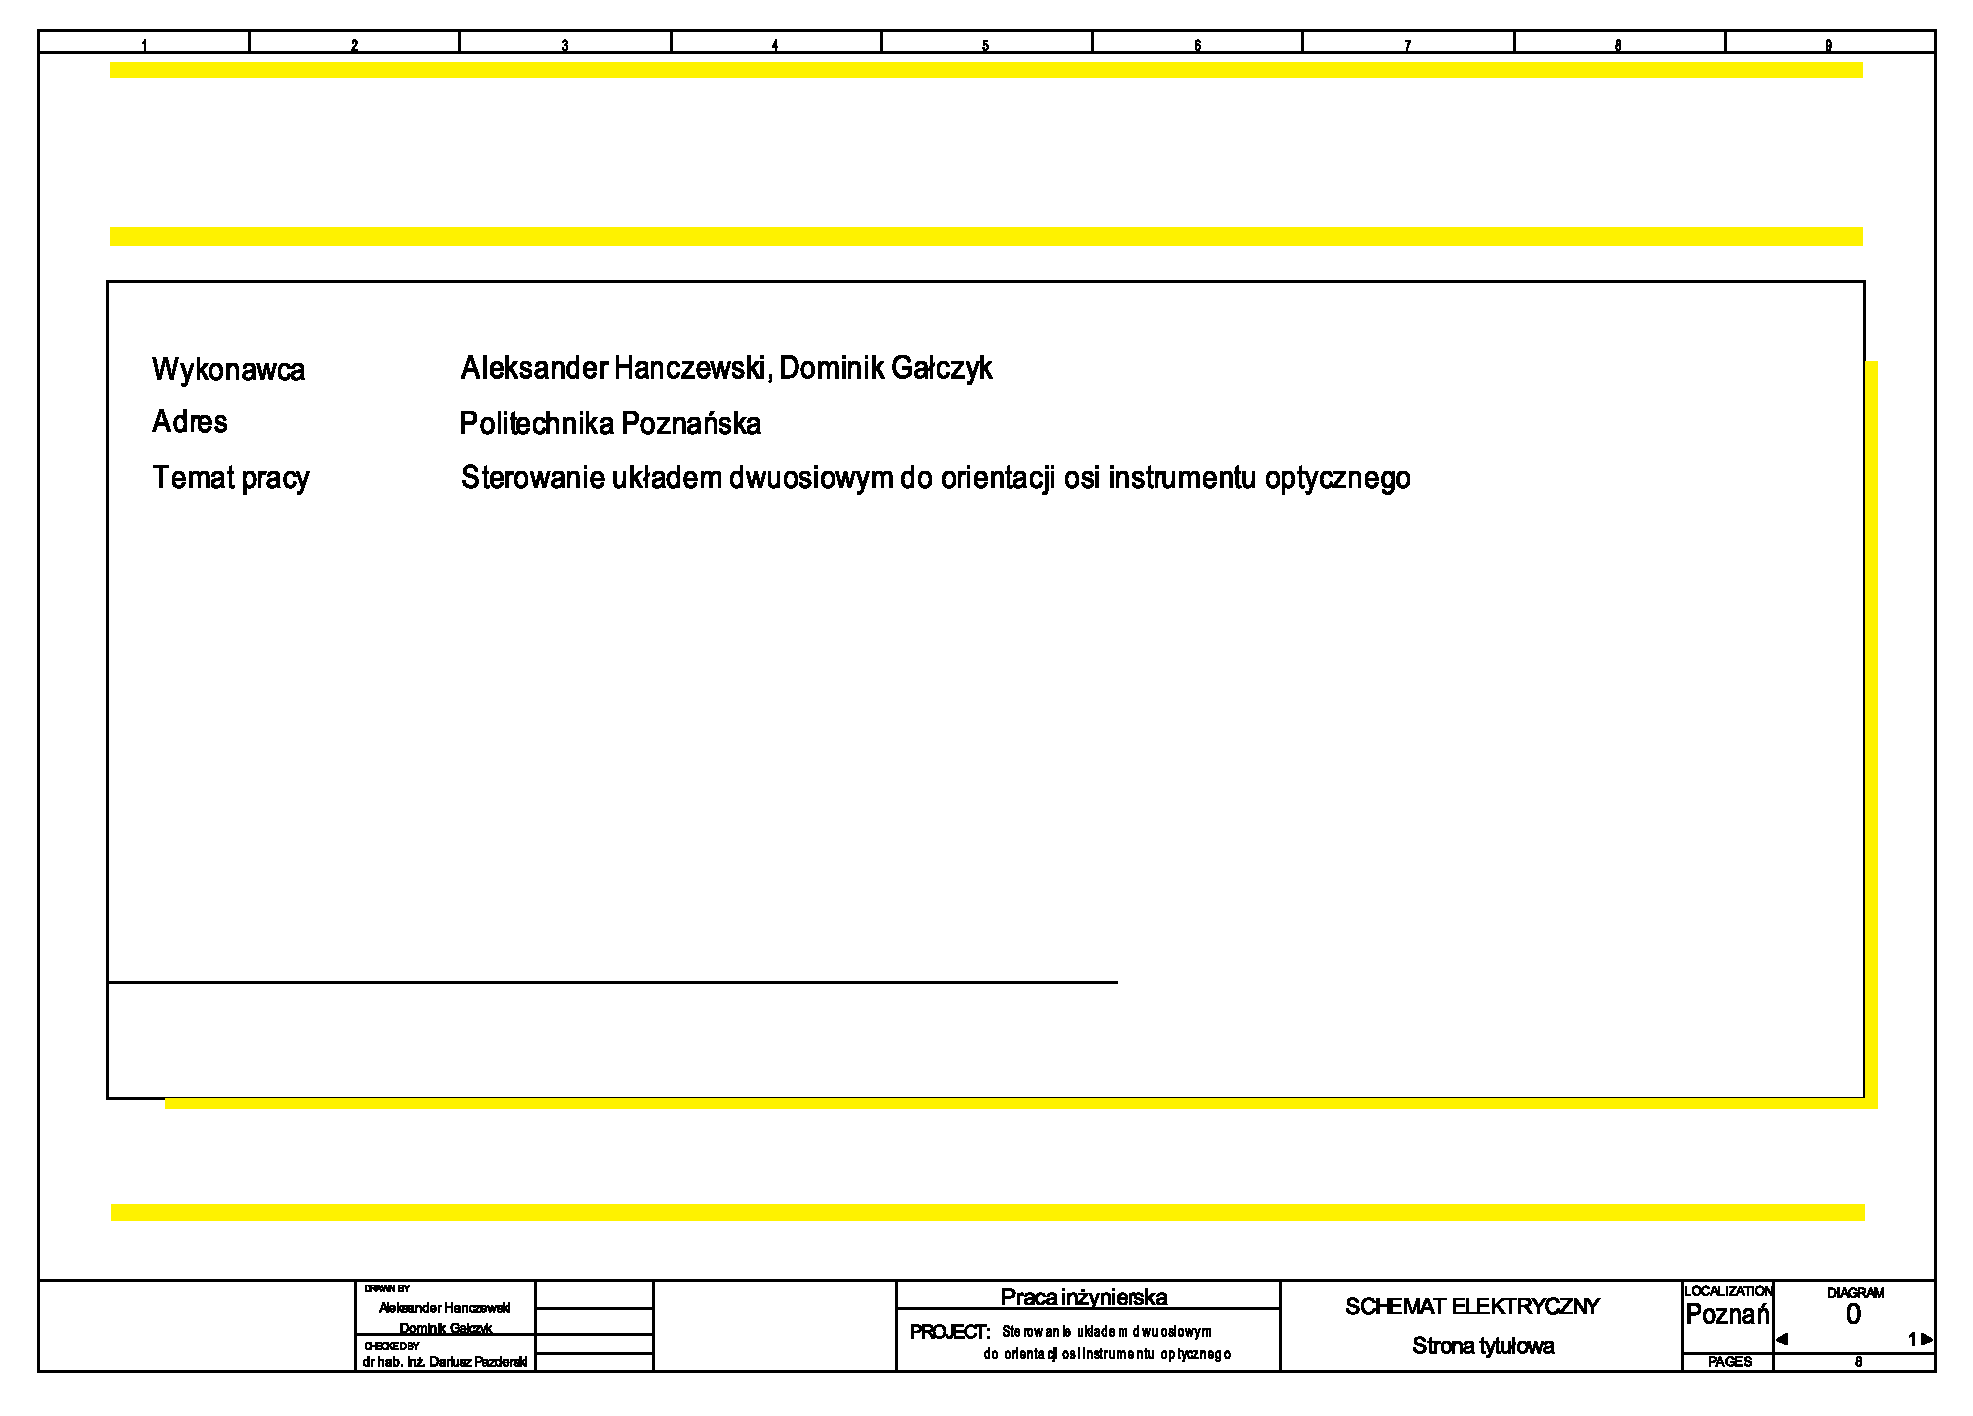
\includegraphics[width=0.85\textwidth]{pictures/schemat_elektryczny/Inżynierka (5).pdf}
\end{figure}

\begin{figure}[H]
    \centering
    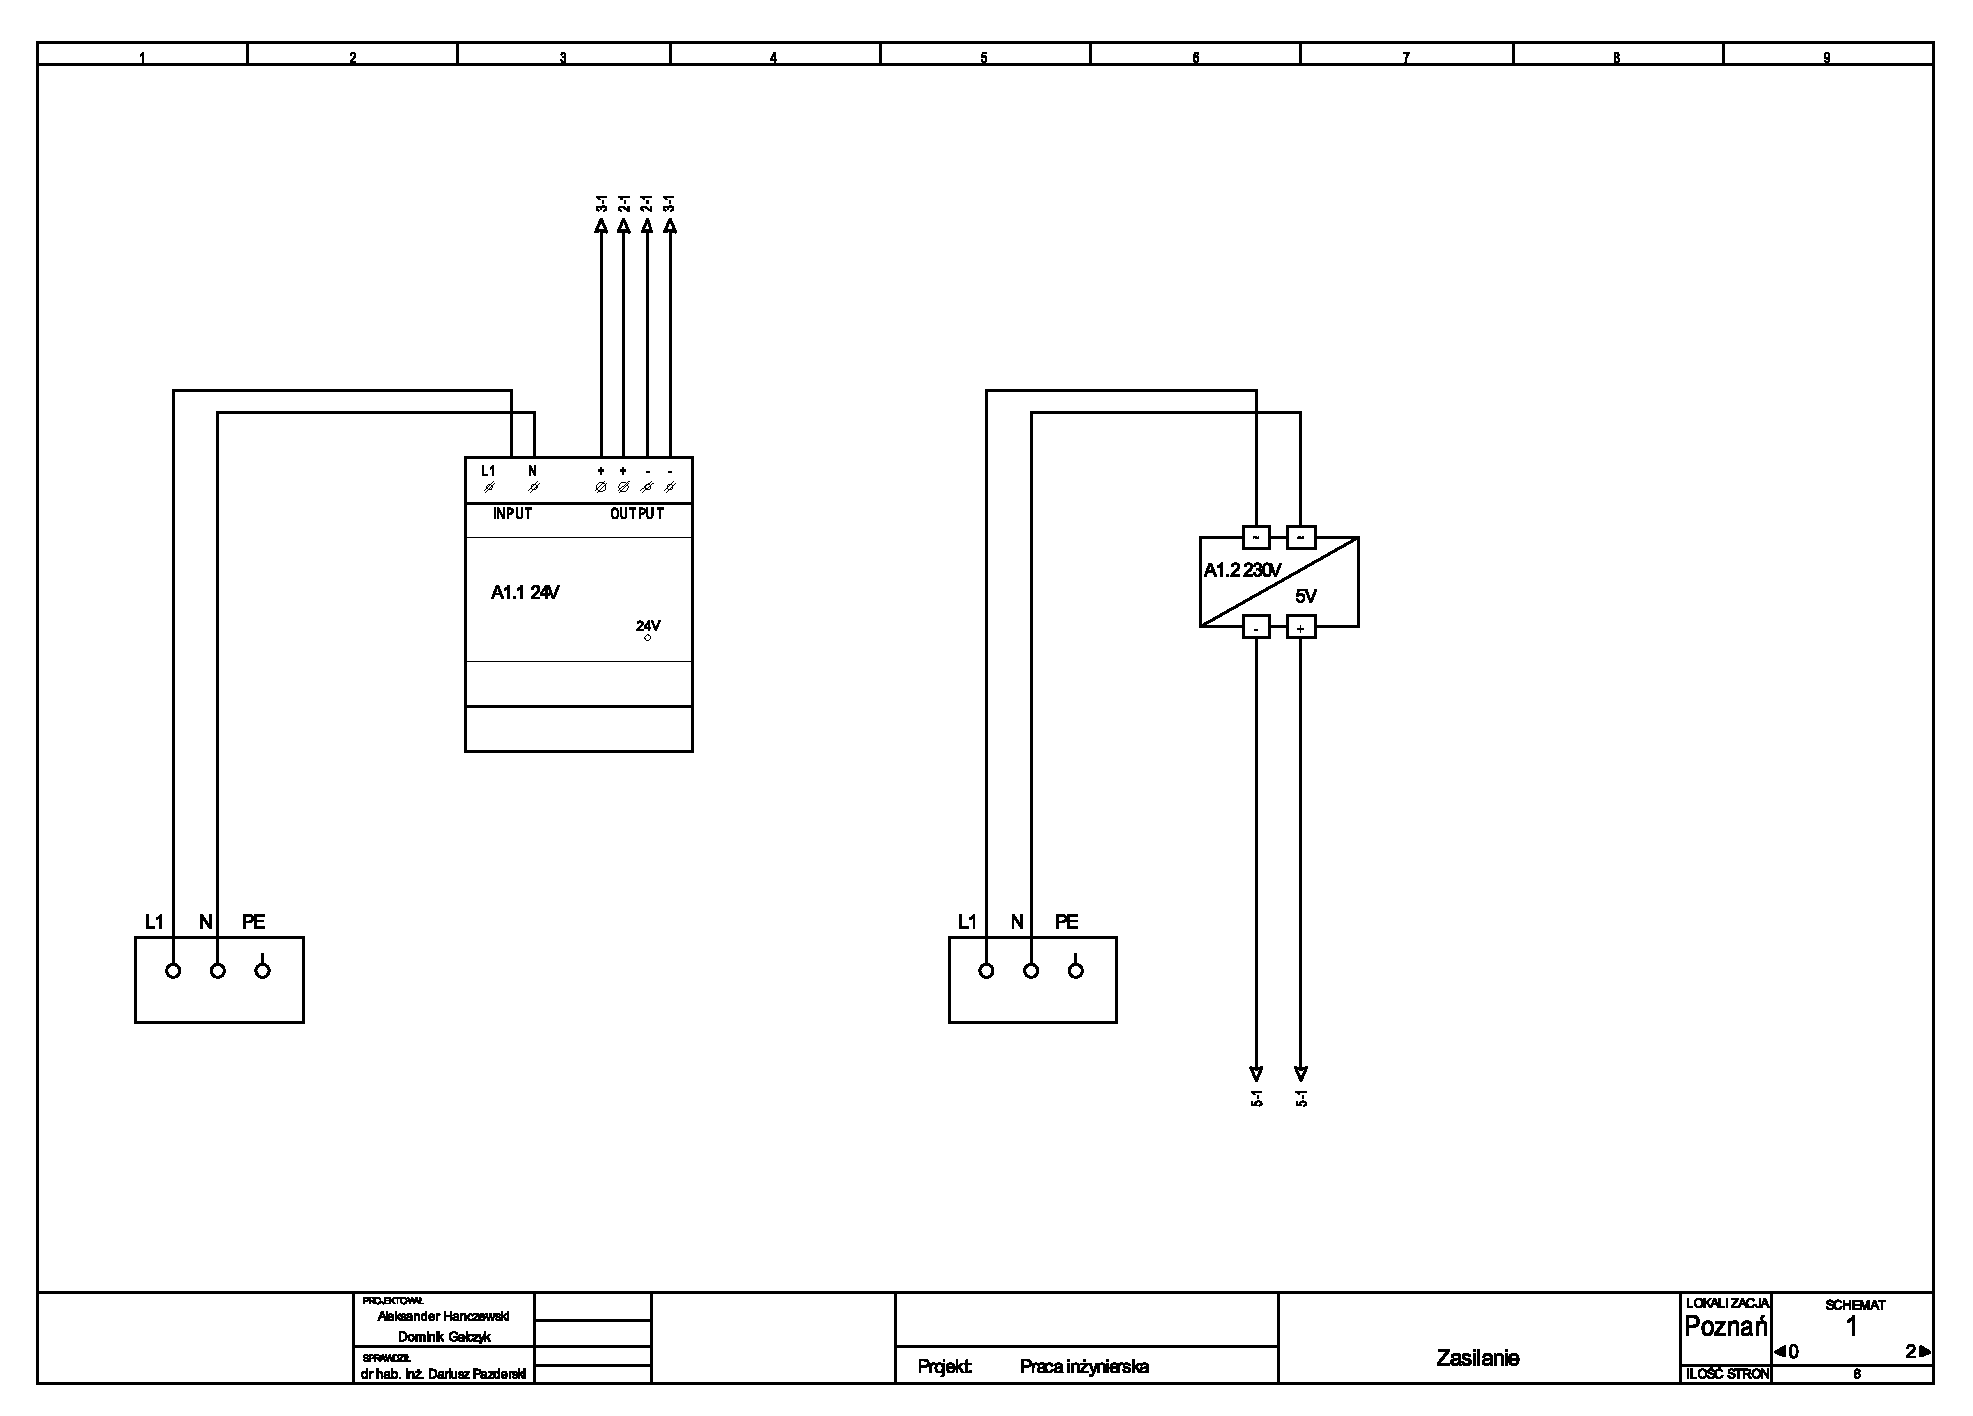
\includegraphics[width=0.85\textwidth]{pictures/schemat_elektryczny/Inżynierka (6).pdf}
\end{figure}

\begin{figure}[H]
    \centering
    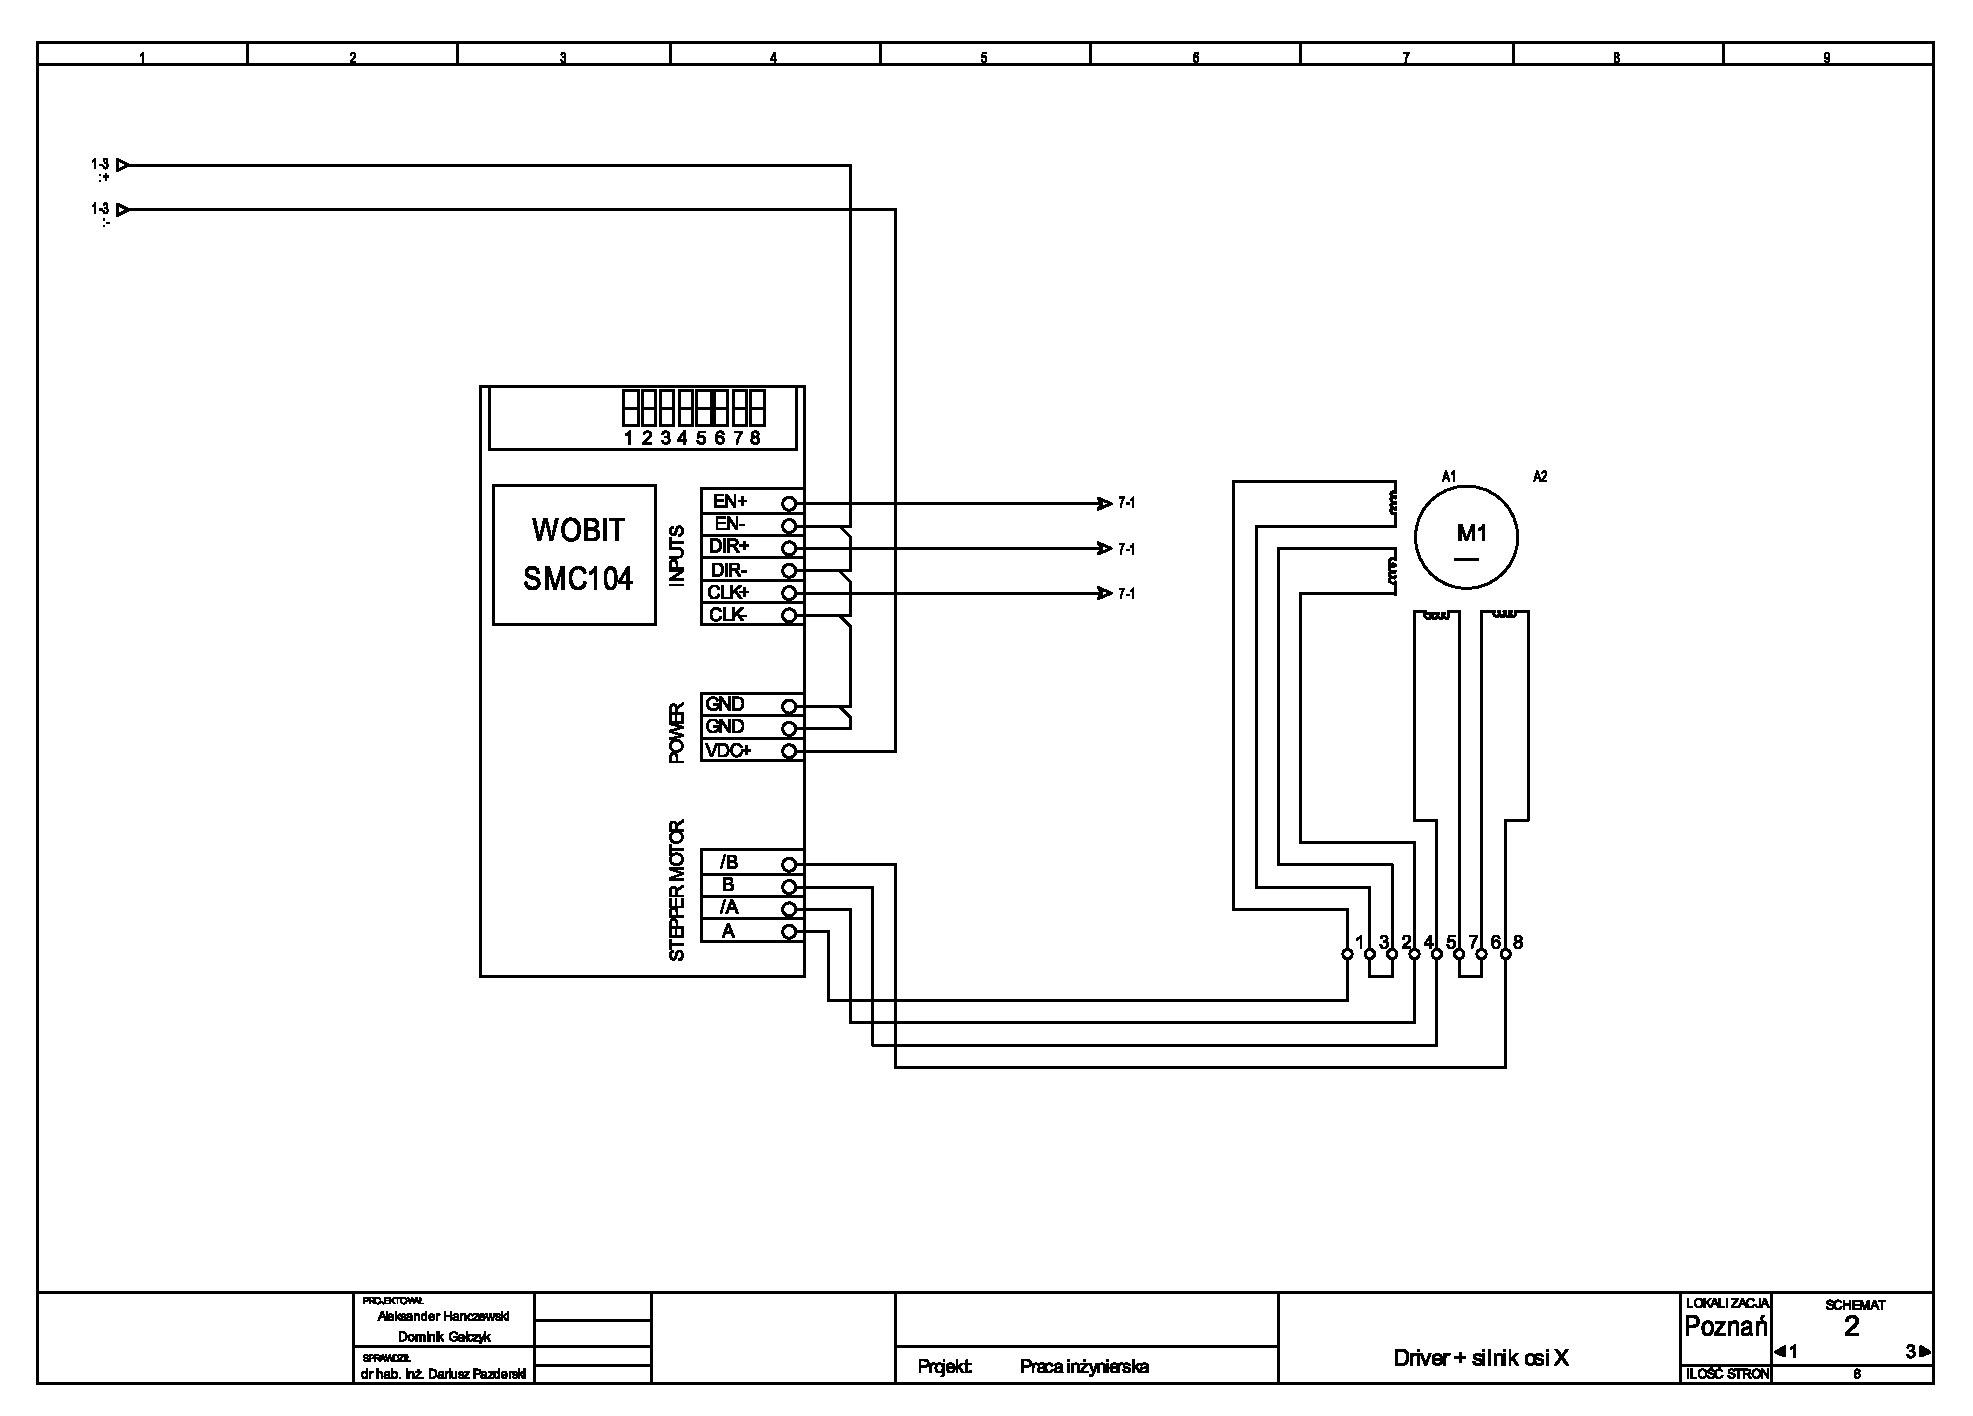
\includegraphics[width=0.85\textwidth]{pictures/schemat_elektryczny/Inżynierka (7).pdf}
\end{figure}

\begin{figure}[H]
    \centering
    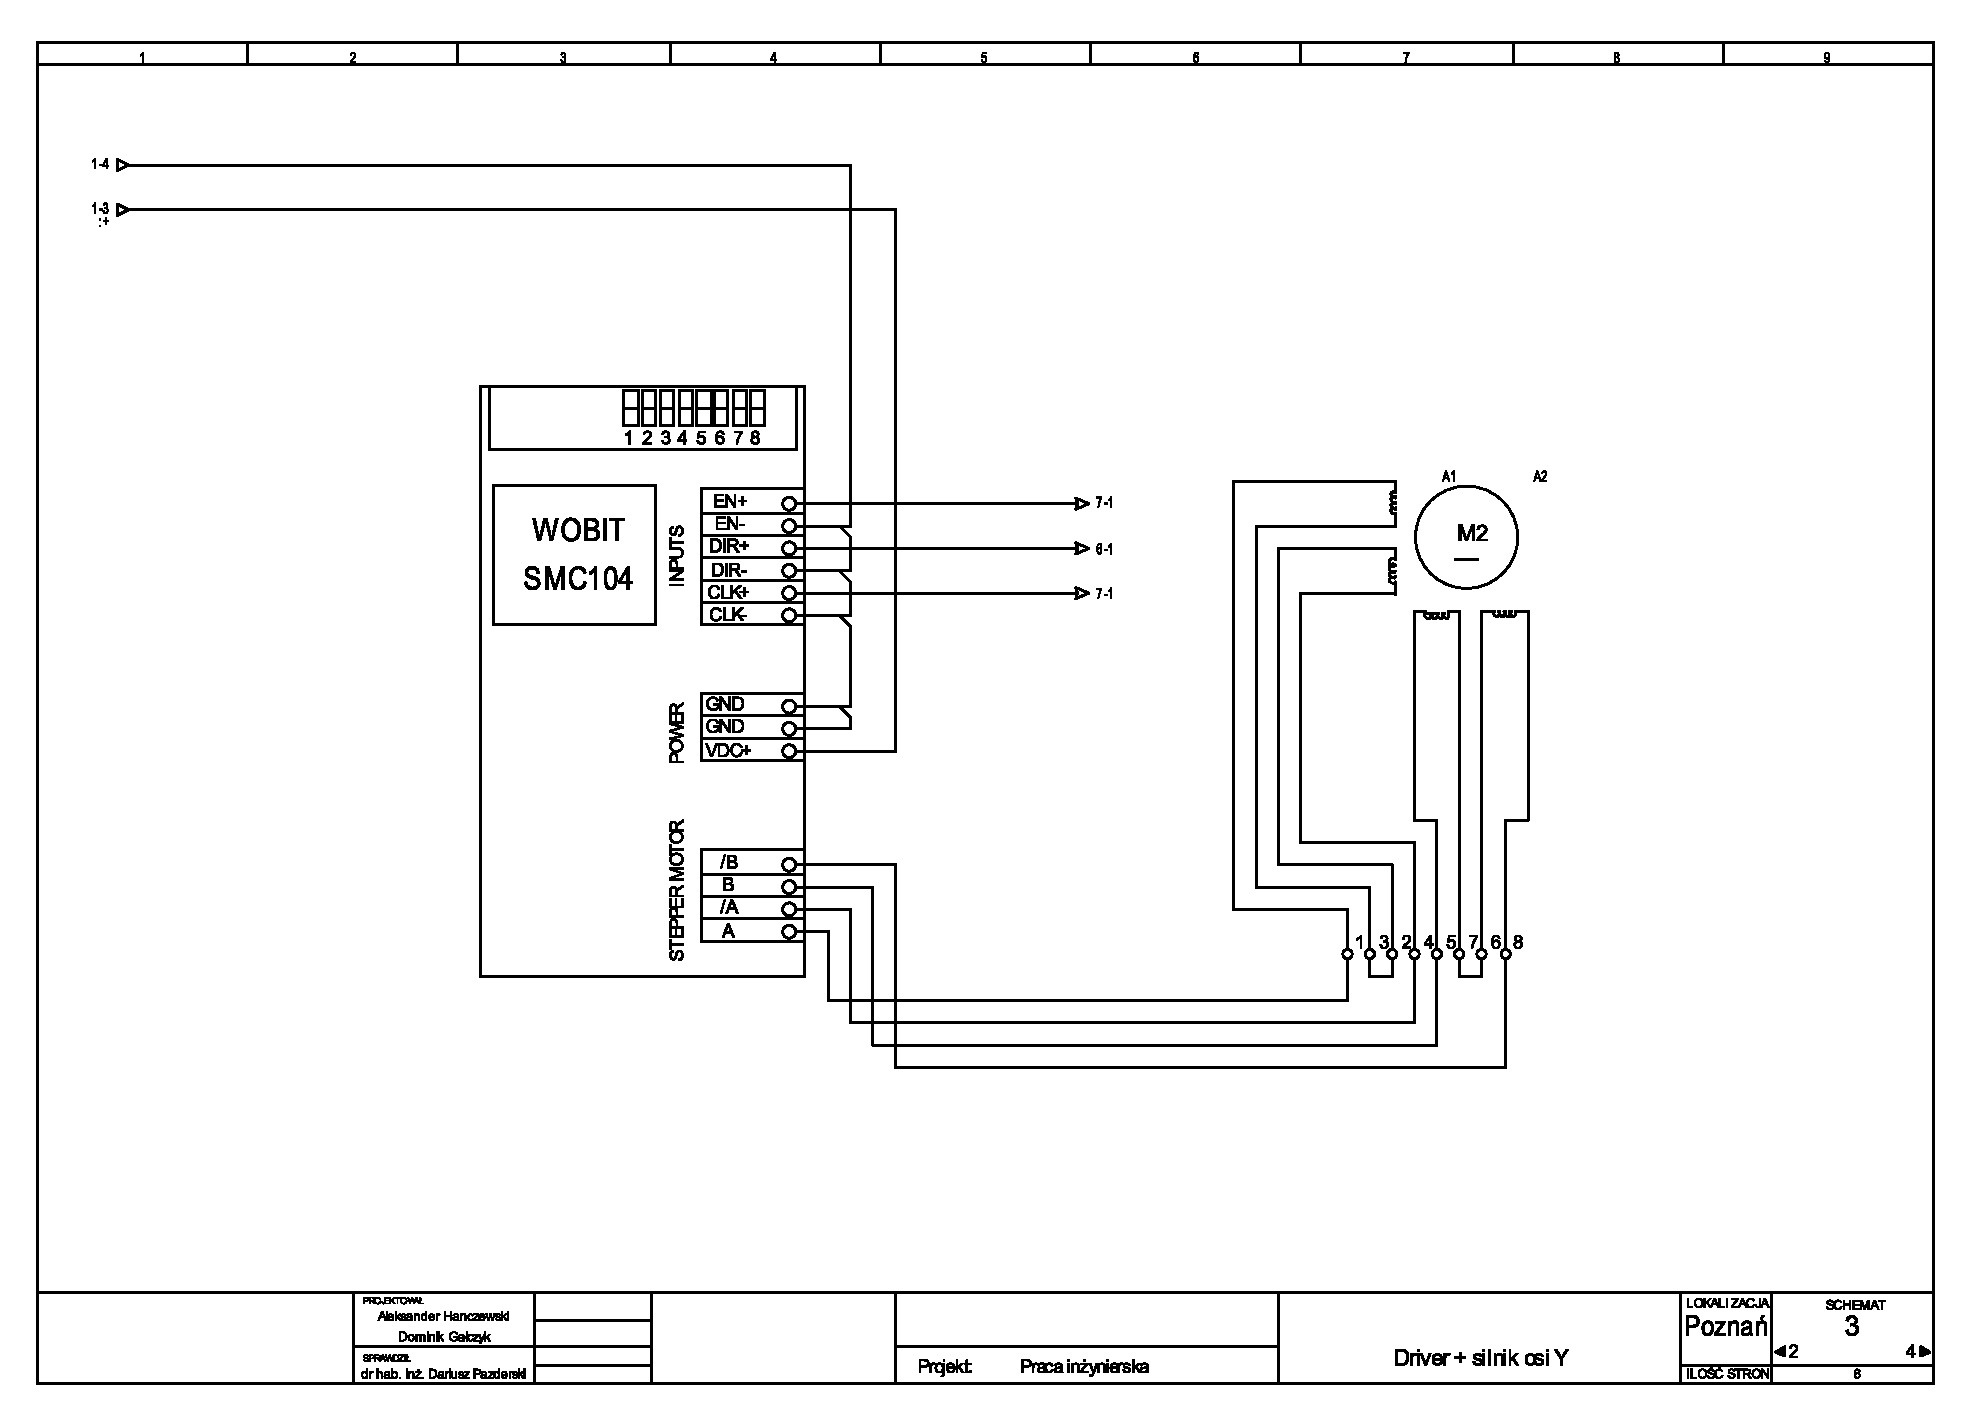
\includegraphics[width=0.85\textwidth]{pictures/schemat_elektryczny/Inżynierka (8).pdf}
\end{figure}

\begin{figure}[H]
    \centering
    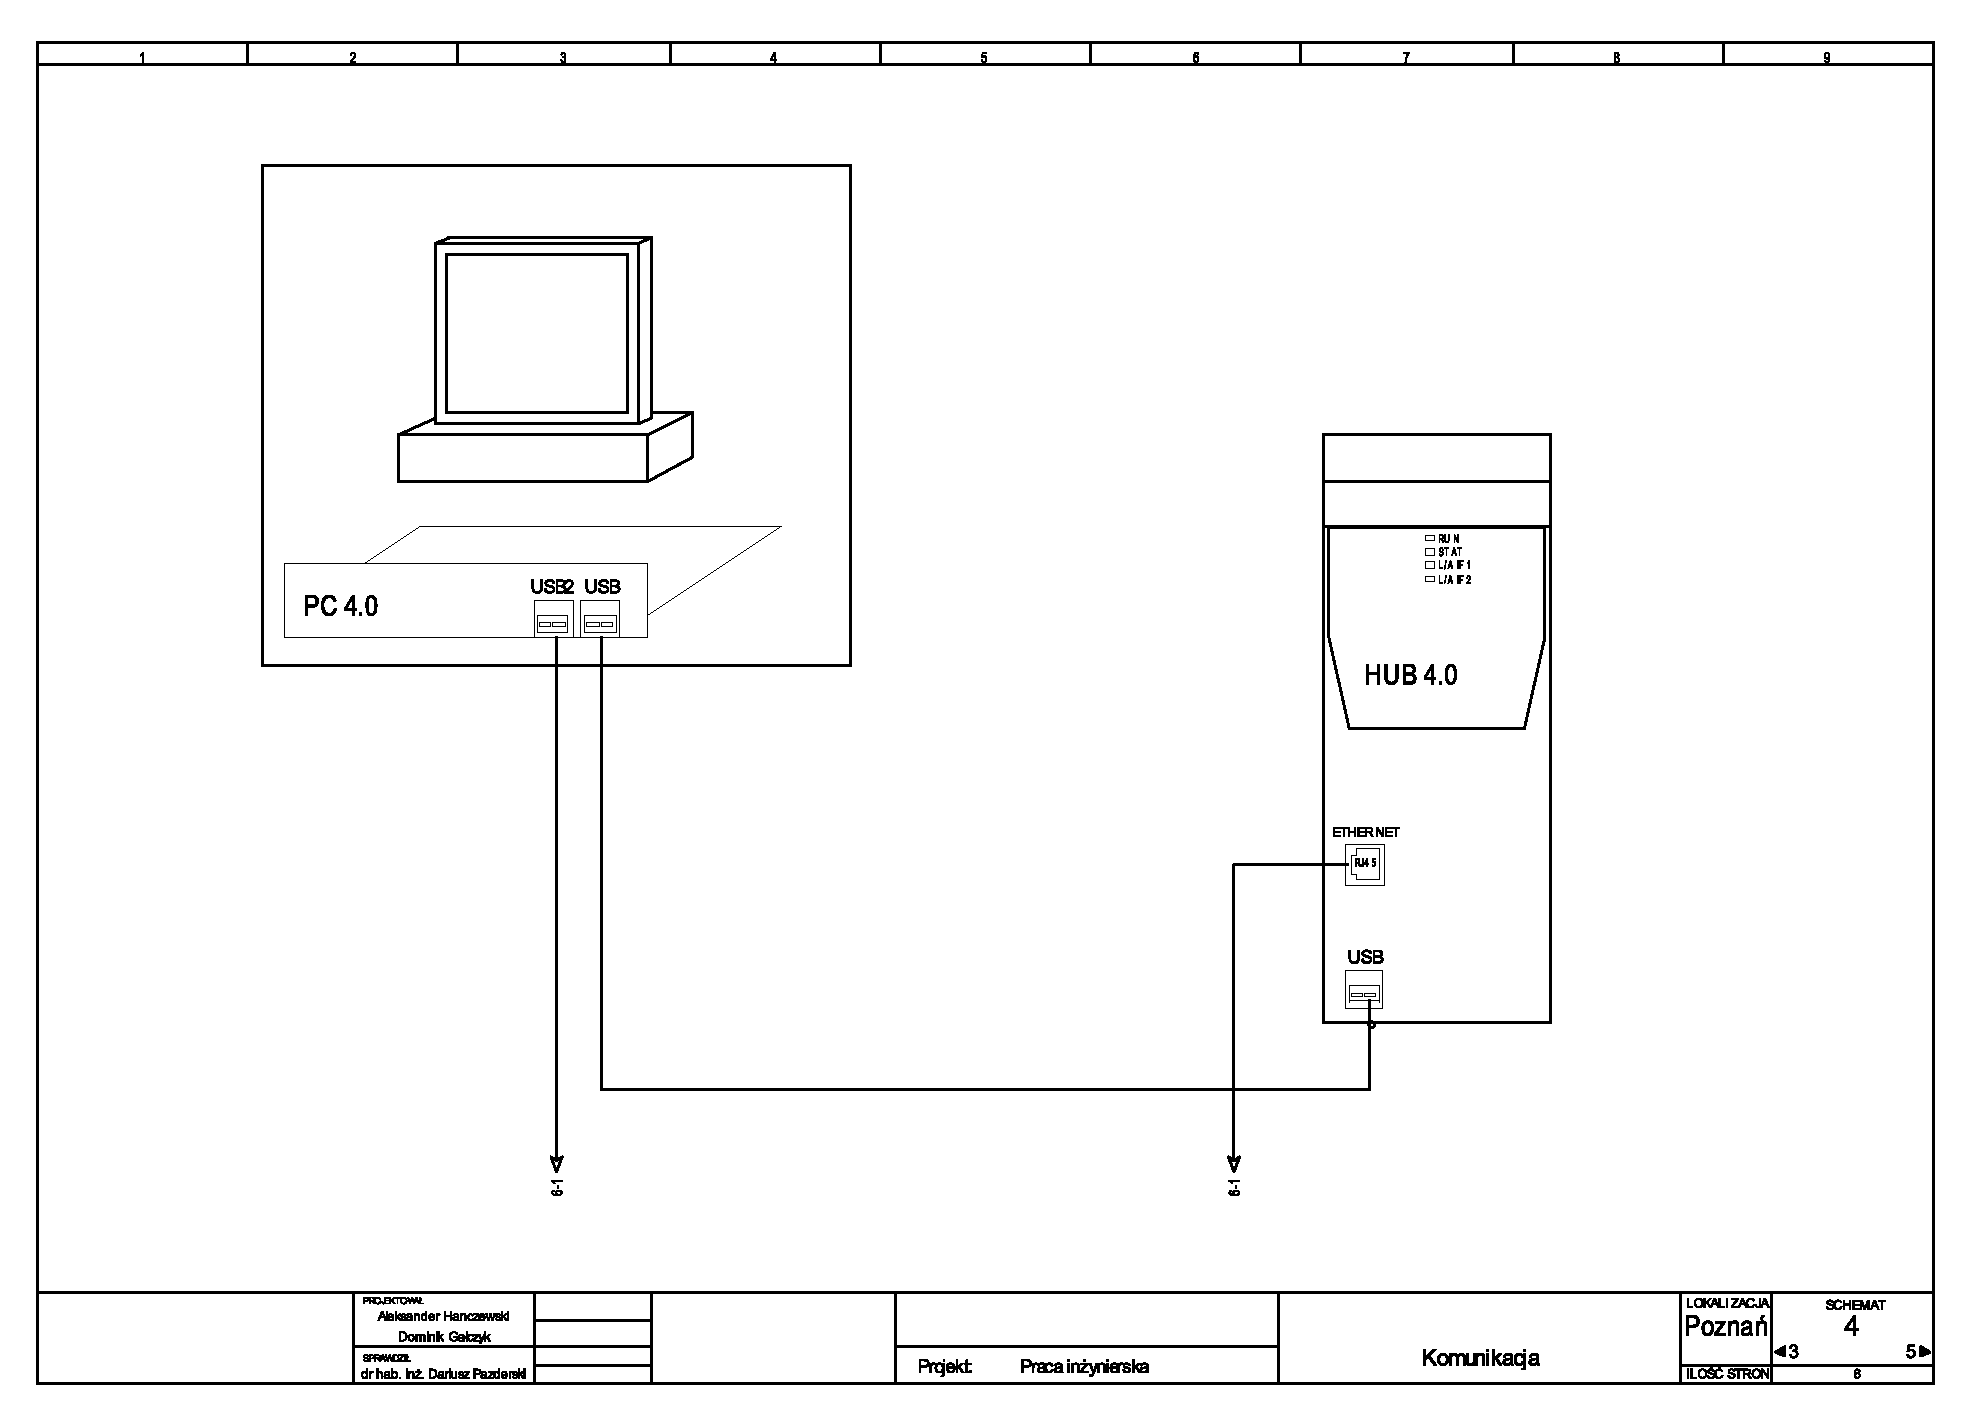
\includegraphics[width=0.85\textwidth]{pictures/schemat_elektryczny/Inżynierka (9).pdf}
\end{figure}

\begin{figure}[H]
    \centering
    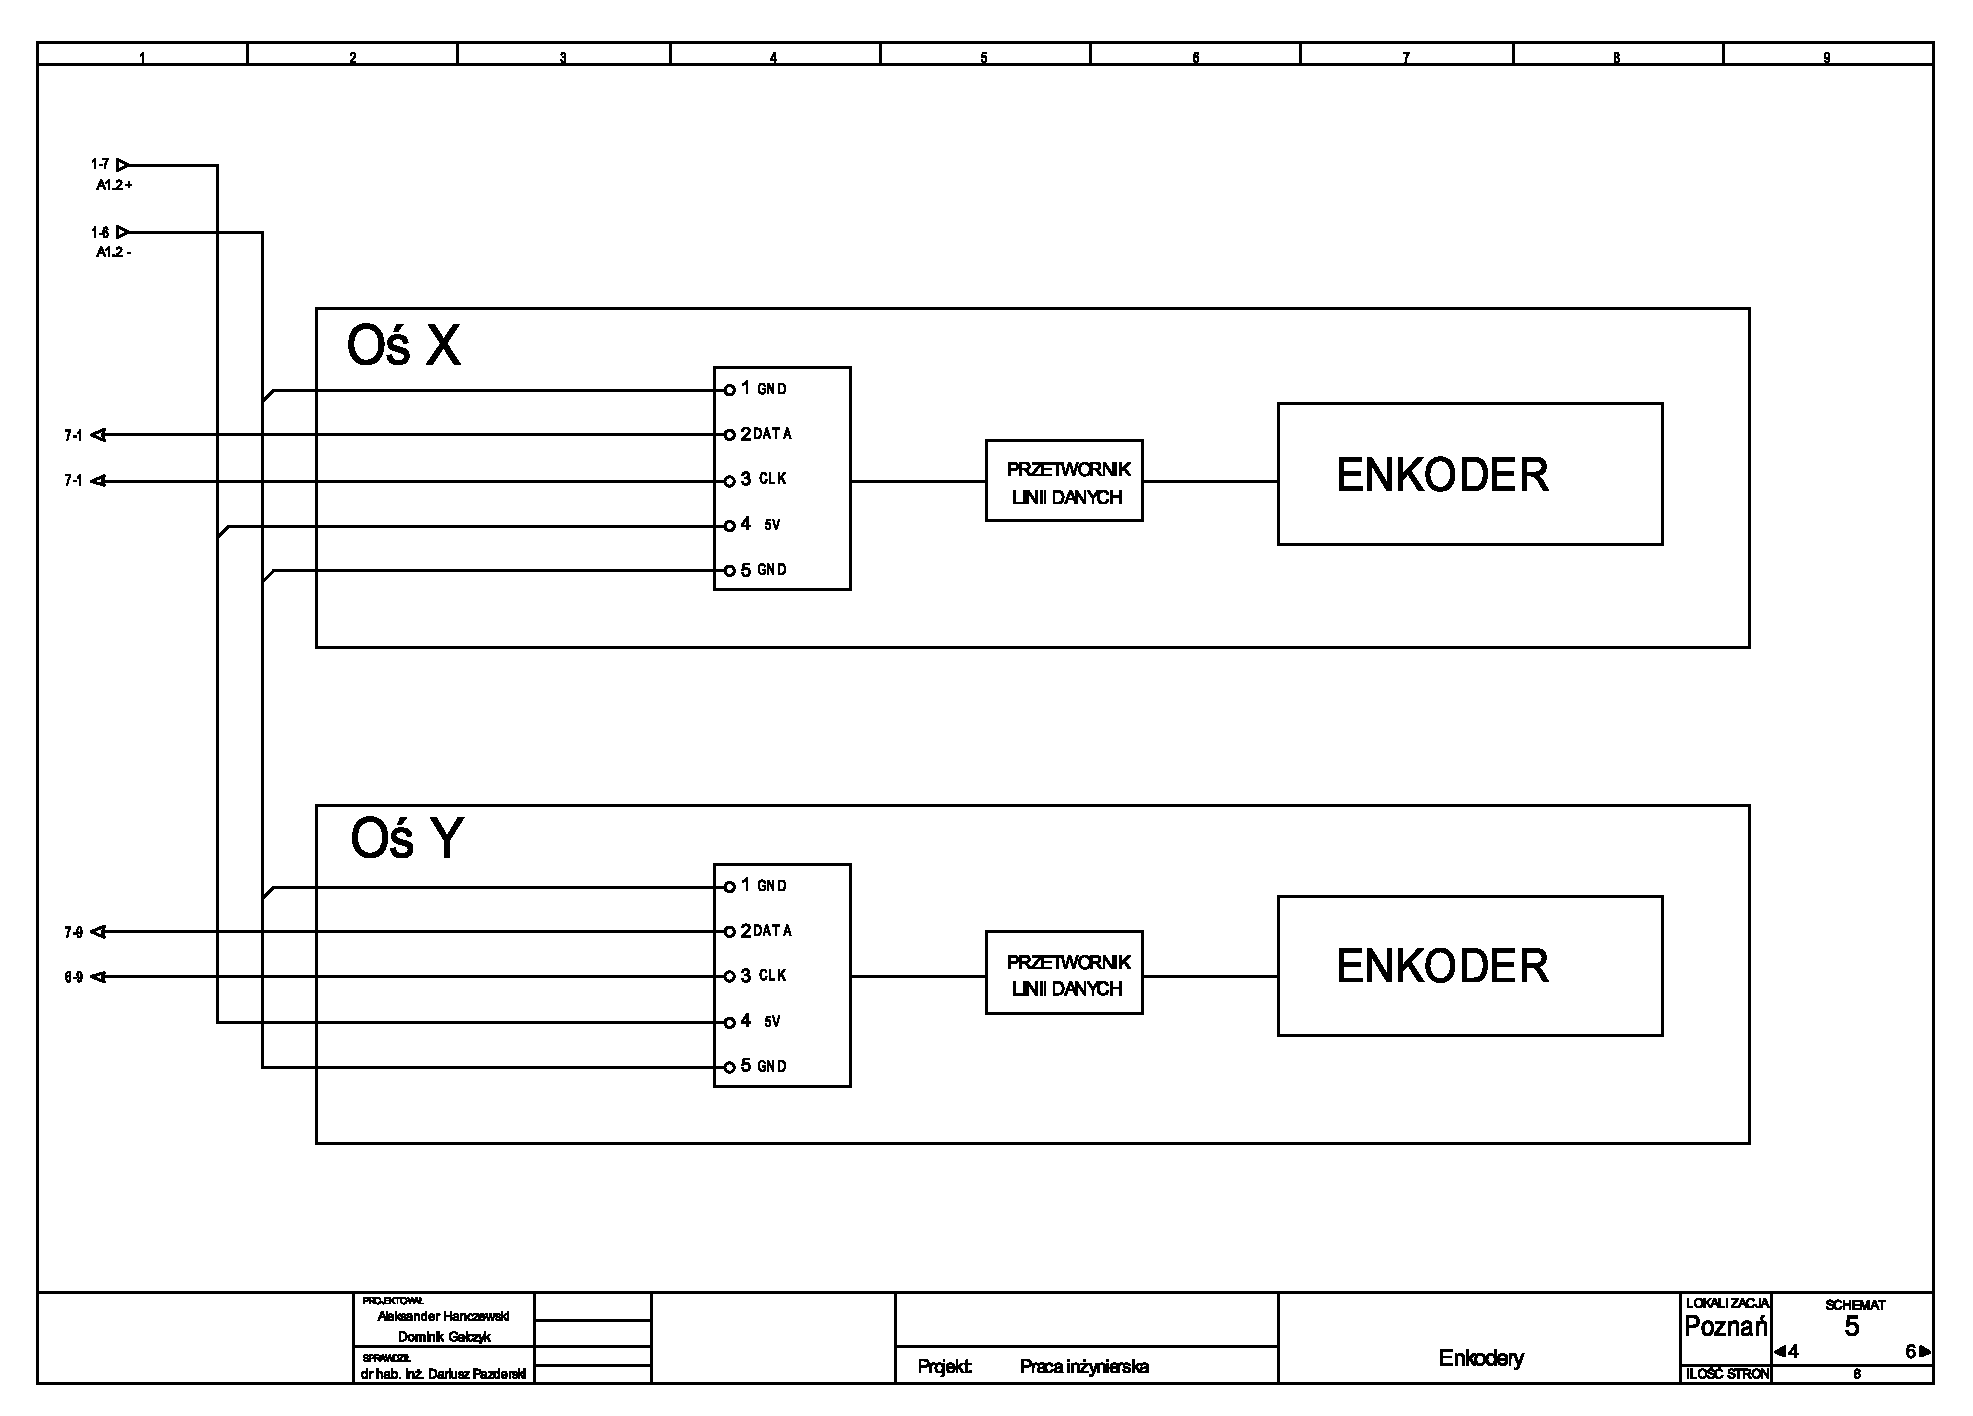
\includegraphics[width=0.85\textwidth]{pictures/schemat_elektryczny/Inżynierka (10).pdf}
\end{figure}

\begin{figure}[H]
    \centering
    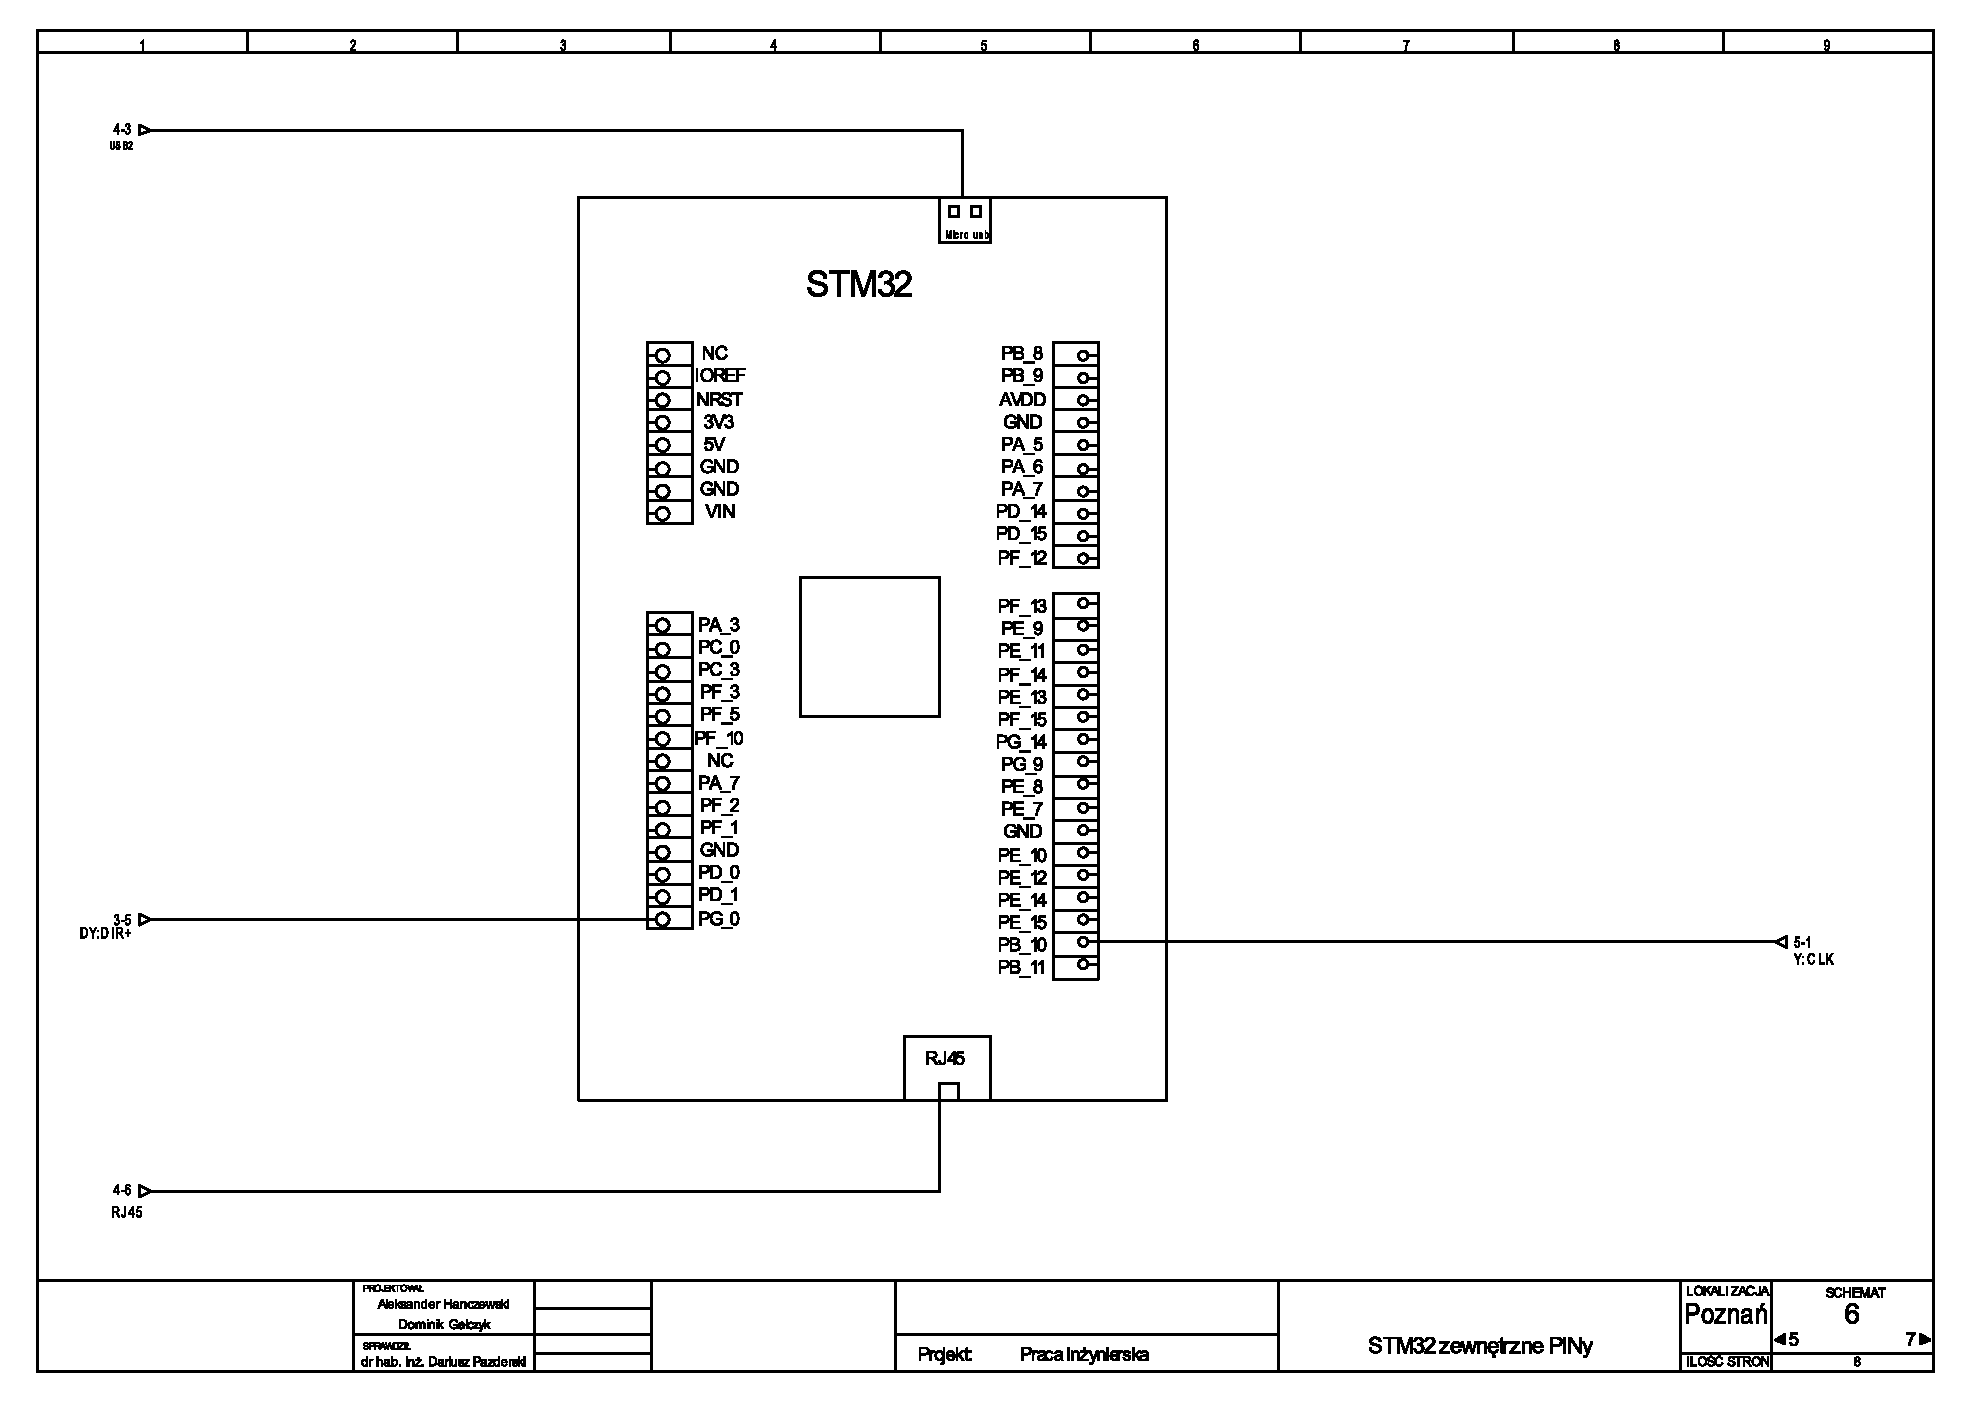
\includegraphics[width=0.85\textwidth]{pictures/schemat_elektryczny/Inżynierka (11).pdf}
\end{figure}

\begin{figure}[H]
    \centering
    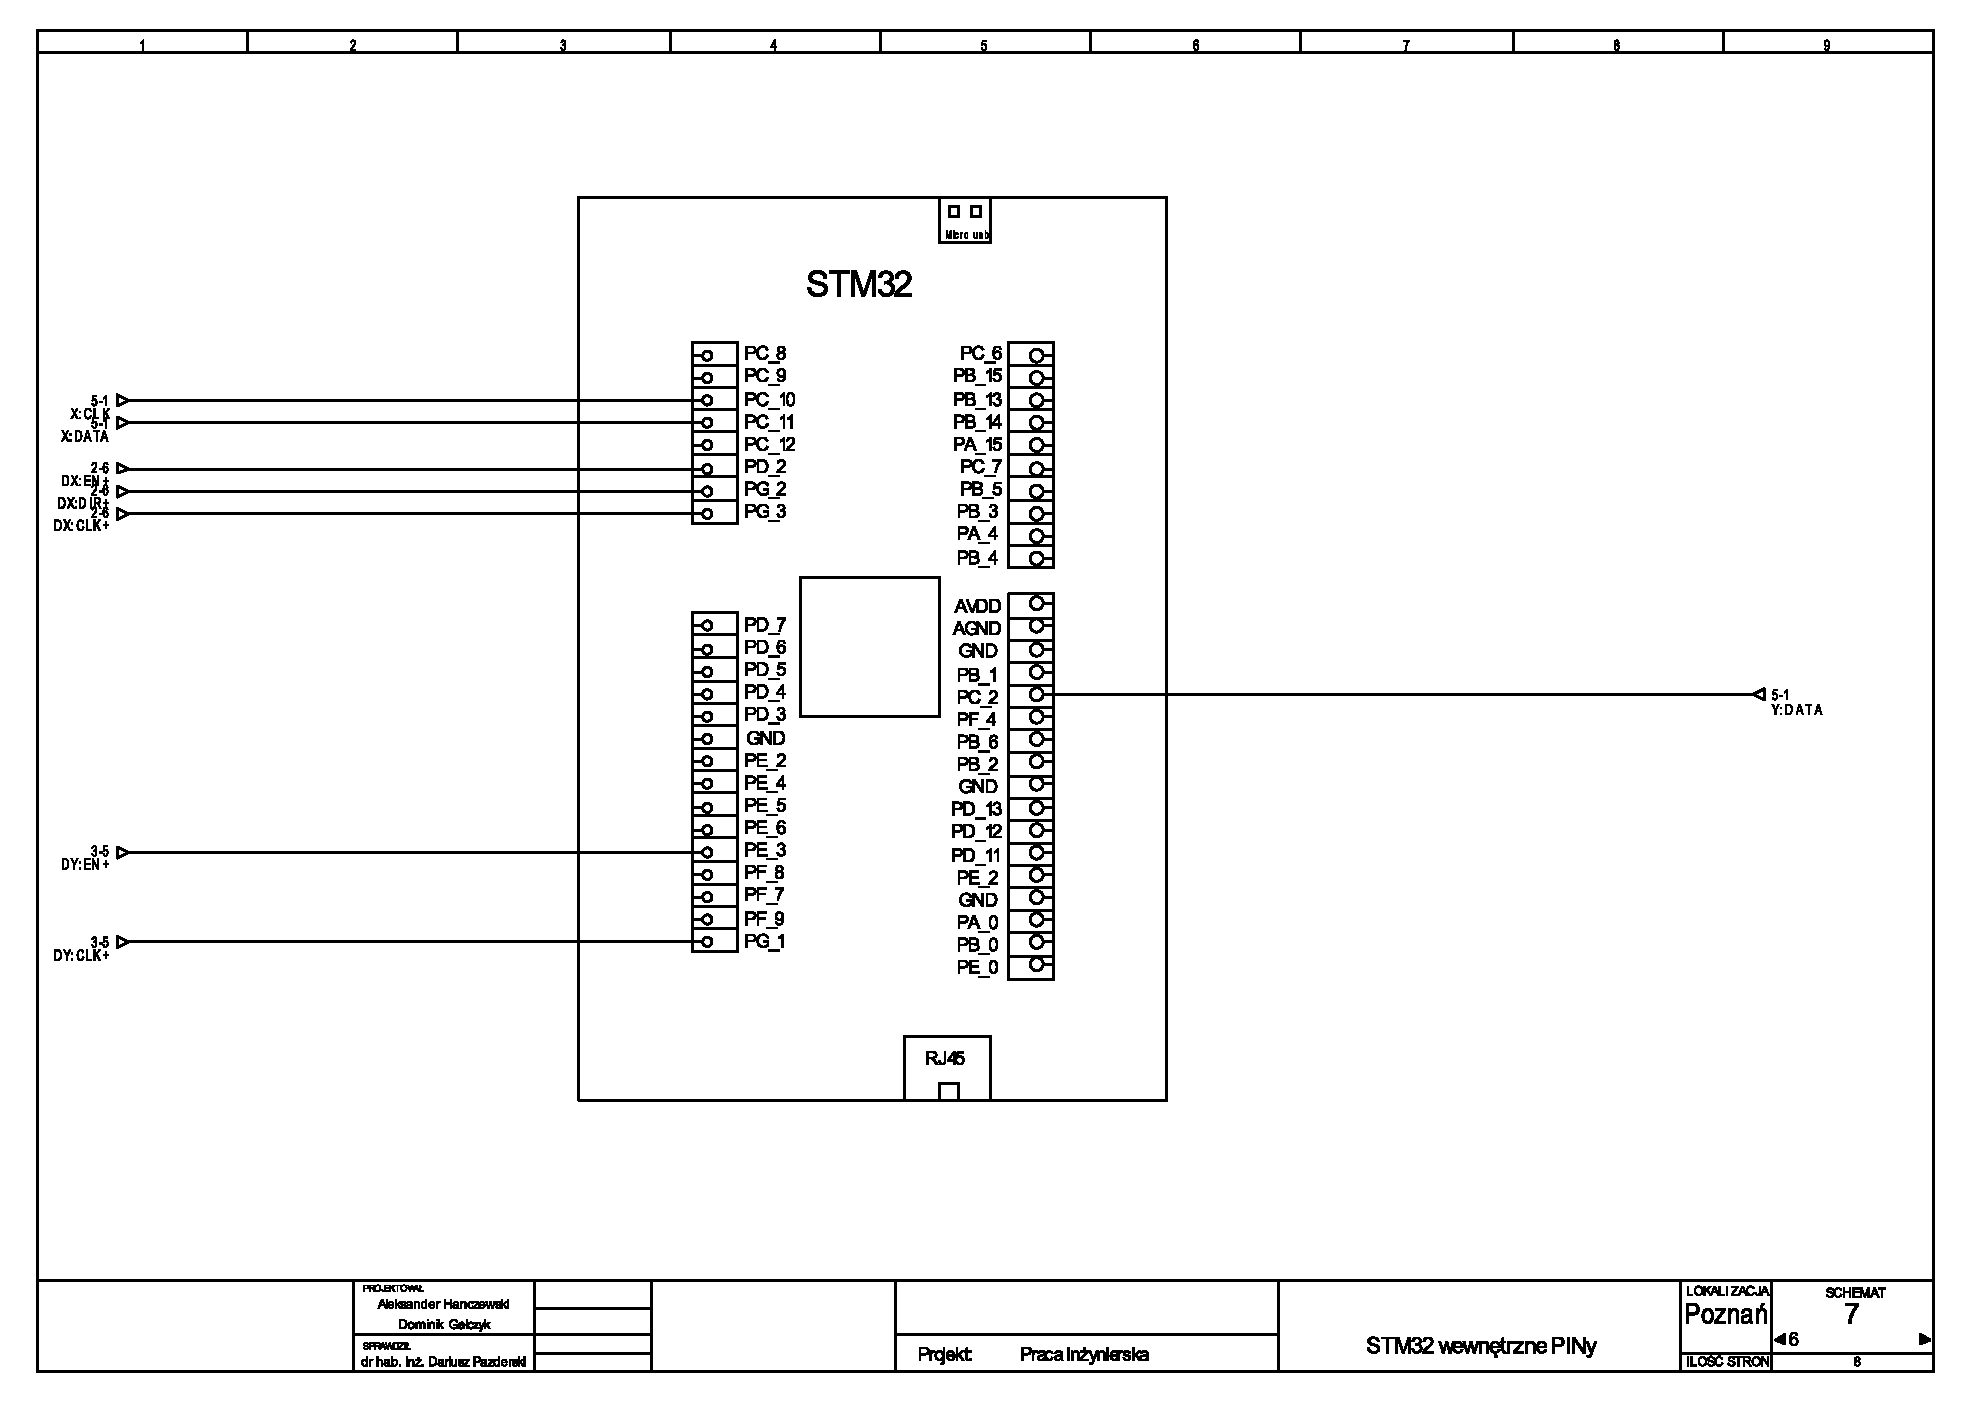
\includegraphics[width=0.85\textwidth]{pictures/schemat_elektryczny/Inżynierka (12).pdf}
\end{figure}

\chapter{Dodatek: Użyte kody w aplikacji}
Repozytorium online z aplikacją webową: \\ https://github.com/DGal02/AirInzynierkaReact2024 \\
Repozytorium online z aplikacją na STM32: \\ https://github.com/DGal02/AirInzynierkaSTM2024

\addtocontents{toc}{\protect\newpage}

\end{document}